\iffalse
\section{Metric Definitions}
\label{sec:metric-details}

\subsection{Stateful-vs-Stateless Gain}
\label{sec:stateful-stateless-gain}

Given a total wall-clock budget $T$ and a split count $N$, compare:
\begin{itemize}
    \item \textbf{Stateful}: one continuous run with budget $T$.
    \item \textbf{Stateless}: $N$ independent runs with budget $T/N$, selecting the best final result.
\end{itemize}
$\mathrm{Gain} = \mathrm{Score}_{\mathrm{stateful}} - \max_i \mathrm{Score}_{\mathrm{stateless}, i}$. A positive gain means accumulated experience is valuable; near-zero gain means a long run behaves like repeated restarts.
\fi

\section{Additional Benchmark and Experiment Details}
\label{sec:additional-benchmark-details}

\subsection{Estimating the With- and Without-Experience Curves}
\label{sec:experience-gain-estimation}

This describes how the two curves in Section~\ref{sec:stateful-stateless-analysis} are estimated. The with-experience curve averages three 12-hour best-so-far curves per task, then averages across tasks. For the without-experience curve, let $u_1,\ldots,u_n$ be the scores of the $n$ independent attempts on a task; at elapsed time $t=k\tau$ we estimate the expected best of $k$ attempts as
\begin{equation}
\hat{u}_{k\tau} = \mathbb{E}_{S}\big[\max_{i\in S} u_i\big],
\end{equation}
where $S$ is sampled uniformly from the $\binom{n}{k}$ size-$k$ subsets of the $n$ attempts. This is the score-valued, without-replacement extension of the pass@$k$ estimator~\cite{chen2021humaneval}; when each $u_i$ is binary, it reduces to the usual pass@$k$ estimate.

\subsection{Gravitational-Wave Case Study Details}
\label{sec:appendix-gw-case-study-details}

\textbf{The selected milestones compress the run into interpretable phase transitions.} Table~\ref{tab:gw-case-study-stages} summarizes the main phases behind the selected milestones rather than every submission. The first selected milestone already passes the protocol and entrypoint checks, generates all five required CSV files on the canonical grids, and obtains a score of 42.8. A subsequent key update raises the score to 47.1, mainly by improving the source dynamics. Around hour 1, another milestone reaches roughly 50 as the agent improves the H1/L1 spectrograms and early H1 alignment in the time domain. These gains reflect standard signal processing: filtering, normalization, windowing in the time-frequency plane, interpolation to the canonical grid, and cropping around the event.

\textbf{The largest score gain comes from the high-weight source-dynamics component.} The largest jump occurs around hours 4--5: the overall score rises from about 52.3 to 59.7, driven almost entirely by the source dynamics subscore (64.2 to 89.0). Because this subtask carries the largest weight, a compact physical model plus calibration produces a large total-score gain. After that point, the agent shifts to H1 waveform tuning, where the H1 time-series subscore climbs from roughly 47 to 95 by the end.

\textbf{The final solution is strong on H1 waveform and source dynamics, but it still leaves room to improve toward a human-standard LIGO-style analysis.} Table~\ref{tab:gw-case-study-subscores} breaks down the final score. GPT-5.5 scores high on H1 waveform reconstruction and the source dynamics but remains weak on the spectrograms and L1 reconstruction. Empirical calibration and parameter search produce a substantial score, but they do not replace a coherent end-to-end pipeline for strain preprocessing, whitening, time-frequency analysis, and waveform alignment across detectors.

\begin{table}[!htbp]
\centering
\footnotesize
\renewcommand{\arraystretch}{1.12}
\setlength{\tabcolsep}{4pt}
\begin{tabular}{lclp{0.46\linewidth}}
\BenchTopRule
Stage & Time & Best score & Main improvement \\
\BenchMidRule
Initial milestones & 0h & 42.8--47.1 & Built a reconstruction pipeline that can be evaluated; replacing a noisy frequency estimate improved the inferred source motion from 51 to 64 (\textbf{+13 pp.}) \\
Early signal processing & 1--4h & 52.3 & Recentered the time-frequency window on the merger; the Hanford detector waveform and both detector spectrograms improved together, raising the best score from 47.1 to 52.3 (\textbf{+5.2 pp.}) \\
Main breakthrough & 4--5h & 59.7 & Calibrated the binary-source model; the orbital velocity and separation score jumped from 64 to 89 (\textbf{+25 pp.}) \\
Late waveform tuning & 5--11.5h & 66.9 & Found the remaining mismatch in the Hanford detector waveform; time-shift alignment and error fitting raised Hanford from 47 to 95 (\textbf{+48 pp.}) \\
Final refinement & 12h & 67.0 & Consolidated final corrections for the Hanford and Livingston detectors; a small Livingston waveform gain raised the aggregate score from 66.9 to 67.0 (\textbf{+0.1 pp.}) \\
\BenchBottomRule
\end{tabular}
\caption{Main phases in the gravitational-wave evolving trajectory. The trajectory shows how the agent refines signal processing, source dynamics, and per-detector waveform reconstruction over the 12-hour run.}
\label{tab:gw-case-study-stages}
\end{table}

\begin{table}[!htbp]
\centering
\footnotesize
\renewcommand{\arraystretch}{1.12}
\setlength{\tabcolsep}{4pt}
\begin{tabular}{lr}
\BenchTopRule
Component & Final subscore \\
\BenchMidRule
H1 time series & 95.0 \\
L1 time series & 57.1 \\
H1 spectrogram & 42.7 \\
L1 spectrogram & 44.7 \\
Velocity/separation & 89.0 \\
\BenchMidRule
Aggregate score & 67.0 \\
\BenchBottomRule
\end{tabular}
\caption{Final subscore composition for the GPT-5.5 gravitational-wave 12h run.}
\label{tab:gw-case-study-subscores}
\end{table}


\clearpage

\subsection{Harness-Level Continuation Ablations}
\label{sec:ablation-experiment-setting}
\label{sec:appendix-ablation-setting}

Long-running agent evaluation depends not only on model capability, but also on how the harness keeps the run alive and carries useful state across many hours. In a 12-hour task, an agent may stop its running unexpectedly due to idleness and need to resume. These continuation mechanisms are therefore part of the practical measurement setup: a weak scaffold can make a capable model stop working on the task, while a stronger scaffold may help the same model keep active and improving. As a supplementary harness-level ablation, we evaluate two such mechanisms, /goal mode and the Ralph loop, under a fixed 12-hour budget with GPT-5.5 and GPT-5.4.

Base uses the standard harness: one continuing agent session, a stop hook to prevent voluntary early exit, and auto-resume for abnormal exits. In /goal mode~\cite{openai2026codexgoals}, the harness prompts the agent to create a task-level goal at the beginning, keep it active during the run, and mark it complete only when the task is validated. The Ralph loop follows the file-backed fresh-context pattern~\cite{huntley2026ralphloop}: each loop starts a new agent invocation on the same workspace, asks it to read and update progress.md, then appends judge feedback to that file before the next loop. It uses up to 100 loops, a 7200-second per-loop cap, and the same 12-hour overall budget. Each cell schedules three runs and reports the mean score over valid runs.

\providecommand{\NA}{\textemdash}
\providecommand{\best}[1]{}
\renewcommand{\best}[1]{\begingroup\bfseries\boldmath #1\endgroup}
\providecommand{\second}[1]{}
\renewcommand{\second}[1]{\underline{#1}}
\providecommand{\sci}[2]{\ensuremath{#1\times 10^{#2}}}
\begin{table*}[t!]
\centering
\footnotesize
\renewcommand{\arraystretch}{1.08}
\setlength{\tabcolsep}{2.5pt}
\resizebox{\textwidth}{!}{%
\begin{tabular}{@{}>{\raggedright\arraybackslash}p{0.34\linewidth}*{6}{>{\centering\arraybackslash}p{0.10\linewidth}}@{}}
\BenchTopRule
\textbf{Task} & \multicolumn{3}{c}{\textbf{GPT-5.5}} & \multicolumn{3}{c}{\textbf{GPT-5.4}} \\
\BenchCMidRule{2-4} \BenchCMidRule{5-7}
 & \textbf{Base} & \textbf{w/ Goal} & \textbf{w/ Ralph} & \textbf{Base} & \textbf{w/ Goal} & \textbf{w/ Ralph} \\
\BenchMidRule
\texttt{portfolio\_\allowbreak{}risk\_\allowbreak{}calibration} & \ensuremath{\mathrm{25.0}} & \second{\ensuremath{\mathrm{27.5}}} & \best{\ensuremath{\mathrm{34.3}}} & \ensuremath{\mathrm{10.7}} & \best{\ensuremath{\mathrm{19.8}}} & \second{\ensuremath{\mathrm{12.2}}} \\
\texttt{storyboard\_\allowbreak{}ad\_\allowbreak{}copywriting} & \ensuremath{\mathrm{77.0}} & \second{\ensuremath{\mathrm{88.3}}} & \best{\ensuremath{\mathrm{97.3}}} & \ensuremath{\mathrm{65.7}} & \second{\ensuremath{\mathrm{78.0}}} & \best{\ensuremath{\mathrm{83.3}}} \\
\texttt{arc\_\allowbreak{}compiler\_\allowbreak{}runtime} & \best{\ensuremath{\mathrm{72.4}}} & \second{\ensuremath{\mathrm{70.6}}} & \ensuremath{\mathrm{52.6}} & \second{\ensuremath{\mathrm{50.0}}} & \ensuremath{\mathrm{47.2}} & \best{\ensuremath{\mathrm{51.2}}} \\
\texttt{battery\_\allowbreak{}soh\_\allowbreak{}rul\_\allowbreak{}anomaly} & \second{\ensuremath{\mathrm{30.2}}} & \ensuremath{\mathrm{23.8}} & \best{\ensuremath{\mathrm{48.8}}} & \best{\ensuremath{\mathrm{14.7}}} & \second{\ensuremath{\mathrm{14.6}}} & \ensuremath{\mathrm{13.4}} \\
\texttt{borden\_\allowbreak{}source\_\allowbreak{}inversion} & \second{\ensuremath{\mathrm{38.5}}} & \ensuremath{\mathrm{32.8}} & \best{\ensuremath{\mathrm{62.2}}} & \ensuremath{\mathrm{8.0}} & \second{\ensuremath{\mathrm{17.3}}} & \best{\ensuremath{\mathrm{23.2}}} \\
\texttt{capecod\_\allowbreak{}plume\_\allowbreak{}reconstruction} & \second{\ensuremath{\mathrm{16.4}}} & \ensuremath{\mathrm{16.0}} & \best{\ensuremath{\mathrm{17.3}}} & \ensuremath{\mathrm{12.6}} & \second{\ensuremath{\mathrm{13.3}}} & \best{\ensuremath{\mathrm{13.7}}} \\
\texttt{combinatorial\_\allowbreak{}games\_\allowbreak{}formalization} & \ensuremath{\mathrm{38.2}} & \best{\ensuremath{\mathrm{45.3}}} & \second{\ensuremath{\mathrm{39.8}}} & \second{\ensuremath{\mathrm{17.8}}} & \ensuremath{\mathrm{13.0}} & \best{\ensuremath{\mathrm{20.2}}} \\
\texttt{ffmpeg\_\allowbreak{}swscale\_\allowbreak{}reimplementation} & \ensuremath{\mathrm{15.3}} & \second{\ensuremath{\mathrm{16.4}}} & \best{\ensuremath{\mathrm{25.2}}} & \ensuremath{\mathrm{13.9}} & \best{\ensuremath{\mathrm{28.3}}} & \second{\ensuremath{\mathrm{21.8}}} \\
\texttt{flt\_\allowbreak{}regular\_\allowbreak{}formalization} & \best{\ensuremath{\mathrm{75.1}}} & \second{\ensuremath{\mathrm{66.7}}} & \ensuremath{\mathrm{58.6}} & \best{\ensuremath{\mathrm{48.3}}} & \second{\ensuremath{\mathrm{43.7}}} & \second{\ensuremath{\mathrm{43.7}}} \\
\texttt{git\_\allowbreak{}rewrite\_\allowbreak{}in\_\allowbreak{}zig} & \ensuremath{\mathrm{18.4}} & \second{\ensuremath{\mathrm{20.5}}} & \best{\ensuremath{\mathrm{22.0}}} & \ensuremath{\mathrm{15.4}} & \best{\ensuremath{\mathrm{18.4}}} & \second{\ensuremath{\mathrm{15.8}}} \\
\texttt{tryst\_\allowbreak{}text\_\allowbreak{}adventure} & \second{\ensuremath{\mathrm{55.7}}} & \best{\ensuremath{\mathrm{56.2}}} & \ensuremath{\mathrm{40.2}} & \best{\ensuremath{\mathrm{44.3}}} & \ensuremath{\mathrm{32.9}} & \second{\ensuremath{\mathrm{42.4}}} \\
\texttt{openttd\_\allowbreak{}transport\_\allowbreak{}ai} & \ensuremath{\mathrm{28.1}} & \best{\ensuremath{\mathrm{39.8}}} & \second{\ensuremath{\mathrm{30.6}}} & \best{\ensuremath{\mathrm{11.9}}} & \ensuremath{\mathrm{1.2}} & \second{\ensuremath{\mathrm{8.1}}} \\
\texttt{pocketbase\_\allowbreak{}backend\_\allowbreak{}architecture} & \best{\ensuremath{\mathrm{62.5}}} & \best{\ensuremath{\mathrm{62.5}}} & \second{\ensuremath{\mathrm{41.7}}} & \second{\ensuremath{\mathrm{20.8}}} & \best{\ensuremath{\mathrm{54.2}}} & \ensuremath{\mathrm{0.0}} \\
\texttt{symbolic\_\allowbreak{}integration\_\allowbreak{}engine} & \best{\ensuremath{\mathrm{44.0}}} & \ensuremath{\mathrm{36.6}} & \second{\ensuremath{\mathrm{37.7}}} & \ensuremath{\mathrm{30.9}} & \best{\ensuremath{\mathrm{63.7}}} & \second{\ensuremath{\mathrm{37.2}}} \\
\BenchMidRule
\textbf{Avg.} & \ensuremath{\mathrm{42.6}} & \second{\ensuremath{\mathrm{43.1}}} & \best{\ensuremath{\mathrm{43.4}}} & \ensuremath{\mathrm{26.1}} & \best{\ensuremath{\mathrm{31.8}}} & \second{\ensuremath{\mathrm{27.6}}} \\
\BenchBottomRule
\end{tabular}%
}
\caption{Harness-level continuation ablation of /goal mode and the Ralph loop. GPT-5.5 and GPT-5.4 are evaluated with Base, Goal, and Ralph settings under the same 12-hour budget; each value is the mean score over valid runs, and the Avg. row averages the displayed task rows. Incomplete cells are detailed in Appendix~\ref{sec:appendix-ablation-setting}. Bold marks the best setting and underlining marks the second-best setting.}
\label{tab:feature_ablation_goal_ralph}
\end{table*}


As shown in Table~\ref{tab:feature_ablation_goal_ralph}, the goal mode and the Ralph loop often outperform the base setting, suggesting that long-horizon agents benefit from harness support that preserves and updates task state across extended runs. In the displayed-task average, GPT-5.5 improves from 42.6 in Base to 43.1 with Goal and 43.4 with Ralph, while GPT-5.4 improves from 26.1 in Base to 31.8 with Goal and 27.6 with Ralph. The gains are not uniform across all tasks and models, so we treat this as an appendix-level harness diagnostic rather than a main result.

Most cells use all three scheduled runs. A few GPT-5.4 cells have fewer valid runs because of intermittent API or network instability: one-run cells are w/ Goal for \texttt{storyboard\_\allowbreak{}ad\_\allowbreak{}copywriting} and \texttt{flt\_\allowbreak{}regular\_\allowbreak{}formalization}, plus w/ Ralph for \texttt{symbolic\_integration\_engine}; two-run cells are \texttt{battery\_\allowbreak{}soh\_\allowbreak{}rul\_\allowbreak{}anomaly} (w/ Goal and w/ Ralph), \texttt{capecod\_\allowbreak{}plume\_\allowbreak{}reconstruction} (w/ Goal), \texttt{combinatorial\_\allowbreak{}games\_\allowbreak{}formalization} (w/ Ralph), \texttt{ffmpeg\_\allowbreak{}swscale\_\allowbreak{}reimplementation} (w/ Goal), \texttt{flt\_\allowbreak{}regular\_\allowbreak{}formalization} (w/ Ralph), \texttt{git\_\allowbreak{}rewrite\_\allowbreak{}in\_\allowbreak{}zig} (w/ Goal), and \texttt{symbolic\_integration\_engine} (w/ Goal). All reported GPT-5.5 cells use the full three runs.


\clearpage

\subsection{Per-Task Design Notes}
\label{sec:task-by-task-design-notes}

This appendix gives per-task design notes for the 134-task \benchmark{} suite.

\begingroup
\scriptsize
\setlength{\tabcolsep}{2pt}
\renewcommand{\arraystretch}{1.0}
\setlength{\LTpre}{4pt}
\setlength{\LTpost}{4pt}
\newcommand{\tasknoterule}{\specialrule{0.12pt}{0.6pt}{0.6pt}}
\begin{longtable}{@{}>{\raggedright\arraybackslash}p{0.20\linewidth}>{\raggedright\arraybackslash}p{0.77\linewidth}@{}}
\BenchTopRule
Task & Design notes \\
\BenchMidRule
\endfirsthead
\BenchTopRule
Task & Design notes \\
\BenchMidRule
\endhead
\BenchMidRule
\multicolumn{2}{r}{\emph{Continued on next page}} \\
\endfoot
\BenchBottomRule
\noalign{\vskip 0.75em}
\caption{Per-task design notes for all 134 \benchmark{} tasks.}\label{tab:task-notes-all}\\
\endlastfoot
\multicolumn{2}{@{}l}{\rule{0pt}{1.2em}\textsc{\scriptsize Systems \& Software Engineering}} \\
\BenchMidRule
\texttt{ann\_\allowbreak{}vector\_\allowbreak{}search\_\allowbreak{}qps} & Replace a brute-force NumPy nearest-neighbor baseline with a high-performance approximate nearest-neighbor implementation under a hard recall constraint. Scored by queries per second. \\
\tasknoterule
\texttt{arc\_\allowbreak{}compiler\_\allowbreak{}runtime} & Implement a complete TypeScript compiler pipeline (lexer, parser, type checker, code generator) for a novel programming language defined by specification documents. \\
\tasknoterule
\texttt{rust\_\allowbreak{}multicrate\_\allowbreak{}reconstruction} & Reconstruct missing Rust implementations across a multi-crate content-addressable storage workspace, given only type signatures and public API contracts. \\
\tasknoterule
\texttt{codeflash\_\allowbreak{}repair\_\allowbreak{}performance} & Diagnose and repair intentionally degraded modules in a Python code-optimization tool spanning CST manipulation, profiling infrastructure, and test harness integration. Scored on both functional correctness and runtime performance. \\
\tasknoterule
\texttt{copier\_\allowbreak{}modular\_\allowbreak{}refactor} & Implement six architectural targets in the Copier Python scaffolding library: structured exceptions, template management, version compatibility, rendering modes, a worker class, and a user-data layer. \\
\tasknoterule
\texttt{dependent\_\allowbreak{}type\_\allowbreak{}checker} & Build a complete dependent type checker in Rust for a subset of Martin-L\"{o}f Type Theory, supporting cumulative universes, Pi/Sigma types, general inductive types with positivity checking, and universe polymorphism. Scored on both correctness and normalization throughput. \\
\tasknoterule
\texttt{entt\_\allowbreak{}graph\_\allowbreak{}module} & Implement seven feature targets in the EnTT C++ entity-component-system framework, including a graph module with adjacency matrix, a task-graph builder with transitive reduction, DOT export, and several core utility additions. \\
\tasknoterule
\texttt{exchange\_\allowbreak{}core\_\allowbreak{}throughput} & Maximize peak throughput of a Java financial matching engine built on the LMAX Disruptor by tuning thread topology, wait strategies, ring-buffer sizing, order-book implementation, and JVM configuration. \\
\tasknoterule
\texttt{ffmpeg\_\allowbreak{}swscale\_\allowbreak{}reimplementation} & Reimplement FFmpeg's libswscale pixel-format conversion and scaling library in Rust, handling multiple pixel formats and scaling algorithms. A correctness-passing scaffold is provided; the agent must optimize for speed via SIMD. \\
\tasknoterule
\texttt{git\_\allowbreak{}rewrite\_\allowbreak{}in\_\allowbreak{}zig} & Reimplement git as a drop-in Zig binary producing identical CLI output, exit codes, and repository state as the C reference implementation. The C source is available for reading but cannot be compiled. \\
\tasknoterule
\texttt{high\_\allowbreak{}performance\_\allowbreak{}object\_\allowbreak{}mapper} & Implement a .NET object-to-object mapping library using expression-tree compilation and IL emission, handling flat/nested mapping, collections, custom type converters, nullables, and inheritance hierarchies. \\
\tasknoterule
\texttt{integer\_\allowbreak{}compression\_\allowbreak{}codec} & Improve a C++ integer compression codec for better compression ratio and decode throughput on uint32 datasets via techniques such as delta encoding, bit-packing, and SIMD vectorization. Exact round-trip correctness is mandatory. \\
\tasknoterule
\texttt{juliet\_\allowbreak{}vulnerability\_\allowbreak{}analyzer} & Implement a deterministic static analyzer that processes structured program facts to detect vulnerabilities across six CWE categories (stack/heap overflow, integer overflow, null dereference, use-after-free, command injection). \\
\tasknoterule
\texttt{libexpat\_\allowbreak{}x86\_\allowbreak{}assembly} & Reimplement the libexpat XML parser entirely in x86-64 assembly, producing an ABI-compatible shared library. No C compiler is available---only assembler, linker, and libc. \\
\tasknoterule
\texttt{odata\_\allowbreak{}query\_\allowbreak{}service} & Complete a .NET OData query processing library: query-string parsing, LINQ expression-tree generation for filtering, multi-field sorting, pagination, field projection, and ASP.NET Core middleware integration. \\
\tasknoterule
\texttt{litestar\_\allowbreak{}infra\_\allowbreak{}refactor} & Implement five async infrastructure subsystems in the Litestar Python web framework: key-value stores with expiry, an event bus, WebSocket listener abstractions, a DTO framework, and a channels pub/sub system. \\
\tasknoterule
\texttt{lua\_\allowbreak{}native\_\allowbreak{}compiler} & Build a Lua 5.4 ahead-of-time native compiler that reads Lua source and emits standalone ELF executables with real x86-64 machine code---not C API call sequences or bytecode dispatch loops. Output must match the reference interpreter byte-for-byte. \\
\tasknoterule
\texttt{mimesis\_\allowbreak{}modular\_\allowbreak{}refactor} & Implement seven refactoring targets in the Mimesis Python fake-data library: a declarative schema class, an enum system with metaclass-driven random selection, and five data providers spanning payments, cryptography, science, internet, and unit systems. \\
\tasknoterule
\texttt{nlohmann\_\allowbreak{}json\_\allowbreak{}modularization} & Implement five feature targets in the nlohmann/json C++ library: UBJSON binary serialization, JSON Merge Patch (RFC 7386), Grisu2 shortest-representation float formatting, a range-based iteration interface, and library metadata macros. \\
\tasknoterule
\texttt{notebook\_\allowbreak{}lossless\_\allowbreak{}compression} & Build a lossless compression pipeline for Jupyter notebooks with a training phase (dictionary learning from a visible corpus) and per-file compression/decompression. Scored by overall compression ratio; byte-exact reconstruction is mandatory. \\
\tasknoterule
\texttt{packer\_\allowbreak{}plugin\_\allowbreak{}datasources} & Implement six targets in HashiCorp Packer's Go plugin ecosystem: address parsing with DNS validation, filesystem-based plugin discovery with checksum verification, HCL2 data-block integration, sensitive value handling, and new template functions. \\
\tasknoterule
\texttt{pocketbase\_\allowbreak{}backend\_\allowbreak{}architecture} & Implement four architectural targets in PocketBase (Go): a chain-based hook/event system, an HTTP router with middleware stacking, a dynamic OAuth2 provider registry, and a regex-based random string generator. \\
\tasknoterule
\texttt{pocketbase\_\allowbreak{}tools\_\allowbreak{}extensions} & Implement four Go utility packages for PocketBase: a REST JSON serializer with nested field picking, a zip archive utility, a cron scheduler with timezone support, and a SQL index parser/builder. \\
\tasknoterule
\texttt{postgres\_\allowbreak{}wire\_\allowbreak{}on\_\allowbreak{}sqlite} & Implement a server that speaks the PostgreSQL wire protocol (v3) using SQLite as the storage backend, handling authentication, simple and extended query protocols, type mapping, transactions, and system catalog queries. Scored by pass rate on PostgreSQL's own test suites. \\
\tasknoterule
\texttt{quic\_\allowbreak{}transport\_\allowbreak{}stack} & Implement a subset of the QUIC transport protocol (RFC 9000): connection establishment, TLS 1.3 key derivation, AEAD encryption, packet number encoding, header protection, and core frame types. \\
\tasknoterule
\texttt{regex\_\allowbreak{}automata\_\allowbreak{}repair} & Repair broken implementations in Rust's regex-automata crate spanning NFA compilation, DFA transition construction, Unicode handling, capture groups, and the hybrid matching engine. \\
\tasknoterule
\texttt{schemathesis\_\allowbreak{}datagen\_\allowbreak{}pipeline} & Implement eight feature targets in the Schemathesis Python API testing framework, including structured HTTP header generation strategies, coverage-phase hooks, discriminator-aware validation and data generation, and schema-driven code generation fixes. \\
\tasknoterule
\texttt{schemathesis\_\allowbreak{}reporting\_\allowbreak{}observability} & Implement five targets in Schemathesis: a post-validation hook system, multi-format test report writers (VCR, HAR, JUnit, NDJSON), pytest plugin integration, and schema-branch-aware example generation. \\
\tasknoterule
\texttt{schemathesis\_\allowbreak{}config\_\allowbreak{}modernization} & Implement six modernization targets in Schemathesis: a TOML-based configuration system with auto-discovery, API namespace reorganization, a metrics framework, transport and response abstractions, and a redesigned check registration system. \\
\tasknoterule
\texttt{stream\_\allowbreak{}processing\_\allowbreak{}engine} & Implement a Rust-based stream processing engine supporting windowed aggregations, filtering, projection, and stateful operators over JSON event streams. Scored on correctness, robustness to malformed input, and throughput. \\
\tasknoterule
\texttt{tls13\_\allowbreak{}handshake\_\allowbreak{}state\_\allowbreak{}machine} & Complete a Python TLS 1.3 protocol state machine that processes handshake message traces, implementing state transitions, key schedule computation, and message validation using a provided crypto API. \\
\tasknoterule
\texttt{vault\_\allowbreak{}sdk\_\allowbreak{}resilience} & Implement five targets in HashiCorp Vault's Go SDK: a string template engine, a fair-share job scheduler, persistent cache storage for agent tokens, certificate utility enhancements, and API client request/response hooks. \\
\tasknoterule
\texttt{vliw\_\allowbreak{}kernel\_\allowbreak{}optimization} & Optimize a VLIW/SIMD kernel generator for correctness and minimum cycle count on a custom architecture simulator. Hard-coded answers for specific inputs are forbidden. \\
\tasknoterule
\texttt{cpu\_\allowbreak{}full\_\allowbreak{}flow} & Work through a full RISC-V CPU design curriculum: ISA emulator implementation, hardware abstraction layer, Verilog processor design, and SoC integration with Verilator simulation. \\
\tasknoterule
\texttt{zstd\_\allowbreak{}api\_\allowbreak{}modernization} & Implement five API evolution targets in Zstandard's C library: stable struct alignment and query functions, a generic parameter-driven compression interface, static allocation support, dictionary enhancements, and memory estimation utilities. \\
\tasknoterule
\texttt{cfzip\_\allowbreak{}compression\_\allowbreak{}engine} & Implement a complete compression engine from scratch in C++17 without external libraries: custom archive format, CLI with streaming mode, dictionary training and use, and integrity verification. Scored on compression ratio, speed, memory usage, and correctness. \\
\BenchMidRule
\multicolumn{2}{@{}l}{\rule{0pt}{1.2em}\textsc{\scriptsize Scientific Problems \& ML}} \\
\BenchMidRule
\texttt{battery\_\allowbreak{}soh\_\allowbreak{}rul\_\allowbreak{}anomaly} & Predict battery state-of-health, remaining useful life, and anomaly type/severity per cycle for unseen cells, given multi-cell degradation training data. Evaluated under distributional shift with regime and calibration changes not present in training. \\
\tasknoterule
\texttt{borden\_\allowbreak{}pump\_\allowbreak{}treat\_\allowbreak{}dispatch} & Build a physics-based groundwater flow model and solve a constrained multi-objective optimization for pump-and-treat remediation on the Borden aquifer, selecting wells, treatment types, and multi-phase schedules under budget and capacity constraints. \\
\tasknoterule
\texttt{borden\_\allowbreak{}source\_\allowbreak{}inversion} & Infer a finite-duration rectangular contaminant source from sparse, noisy monitoring-well observations in a 3D hydrogeological scene. The agent must implement its own forward model and inversion optimizer from scratch. \\
\tasknoterule
\texttt{borden\_\allowbreak{}sensor\_\allowbreak{}fault\_\allowbreak{}diagnosis} & Classify sensor faults (spikes, drift, stuck-at-zero, unit errors, etc.) versus true plume arrivals in groundwater monitoring records using physics-informed checks such as travel-time ordering and neighbor-well consistency. \\
\tasknoterule
\texttt{bridge\_\allowbreak{}gnss\_\allowbreak{}state\_\allowbreak{}forecast} & Process dirty bridge GNSS displacement time series (timestamp jitter, duplicates, spikes, drift) and produce cleaned reconstruction, state estimates, and short-term displacement forecasts. \\
\tasknoterule
\texttt{capecod\_\allowbreak{}plume\_\allowbreak{}reconstruction} & Reconstruct a multi-analyte groundwater plume from sparse monitoring wells: predict concentrations at withheld locations and times, compute plume metrics, and propose an optimal monitoring network under budget constraints. \\
\tasknoterule
\texttt{vsg\_\allowbreak{}stability\_\allowbreak{}parameter\_\allowbreak{}optimization} & Integrate current-limited Virtual Synchronous Generators into the IEEE 39-bus power system, generate transient stability data, build a physics-informed neural network, and train a reinforcement learning agent to optimize VSG parameters. \\
\tasknoterule
\texttt{cylinder\_\allowbreak{}wake\_\allowbreak{}prediction} & Implement a CPU-only 2D cylinder wake solver for the incompressible Navier-Stokes equations. Evaluated on unseen Reynolds numbers and domain configurations; scored on velocity-field accuracy, pressure-field accuracy, and flow-regime prediction. \\
\tasknoterule
\texttt{dabic\_\allowbreak{}gravity\_\allowbreak{}inversion} & Implement the D-ABIC regularization method for 3D gravity inversion within the SimPEG framework, run on both synthetic and real Vinton salt dome data under L0 and L1 sparse norms, and compare against a Hamiltonian Monte Carlo baseline. \\
\tasknoterule
\texttt{noisy\_\allowbreak{}product\_\allowbreak{}matching\_\allowbreak{}pipeline} & Determine whether pairs of product listings from different sources refer to the same real-world item, given noisy and incomplete attributes. Evaluated on hidden variants with different noise characteristics and data scales; no ground-truth labels are available during development. \\
\tasknoterule
\texttt{neural\_\allowbreak{}net\_\allowbreak{}weight\_\allowbreak{}recovery} & Reconstruct the correct layer ordering of a neural network from 97 shuffled weight files and input-output historical data, using dimensional constraints and reconstruction-error analysis. \\
\tasknoterule
\texttt{nanophotonic\_\allowbreak{}simulation\_\allowbreak{}reproduction} & Reproduce published nanophotonic simulation results (multi-source electromagnetic field distributions) from a research paper, implementing the solver from scratch using only NumPy. \\
\tasknoterule
\texttt{ftir\_\allowbreak{}polymer\_\allowbreak{}identification} & Identify polyimide monomers from FTIR spectra by correlating IR absorption peaks with functional groups, optionally aided by quantum chemistry simulations. Submission attempts are rate-limited to prevent brute-force enumeration. \\
\tasknoterule
\texttt{molecular\_\allowbreak{}property\_\allowbreak{}regression} & Predict molecular properties from graph representations without graph neural network libraries. Evaluated on multi-domain data with perturbations that penalize solutions overfitting to the development distribution. \\
\tasknoterule
\texttt{graph\_\allowbreak{}node\_\allowbreak{}classification} & Implement graph neural networks from scratch using only base PyTorch for semi-supervised node classification on an unseen graph under CPU-only constraints. \\
\tasknoterule
\texttt{gravitational\_\allowbreak{}wave\_\allowbreak{}signal\_\allowbreak{}detection} & Reproduce the LIGO GW150914 gravitational-wave detection pipeline: whitening, bandpass filtering, matched filtering against a numerical-relativity template, time-frequency analysis, and residual computation. \\
\tasknoterule
\texttt{herbal\_\allowbreak{}depression\_\allowbreak{}target\_\allowbreak{}screening} & Screen active components and protein targets for four traditional Chinese medicine herbs used in depression treatment, producing component lists, target mappings, disease-target intersections, and a PPI network visualization. \\
\tasknoterule
\texttt{polyimide\_\allowbreak{}homo\_\allowbreak{}lumo\_\allowbreak{}prediction} & Compute HOMO/LUMO energies of polyimide repeating units using DFT calculations, analyze substituent and conjugation effects on electronic properties, and identify the monomer pair with the widest band gap. \\
\tasknoterule
\texttt{industrial\_\allowbreak{}anomaly\_\allowbreak{}detection} & Detect anomalies in multivariate industrial sensor time series using only classical ML libraries. Evaluated on hidden variants including time-series crops, reversals, and normal-only segments to prevent hard-coding. \\
\tasknoterule
\texttt{bipedalwalker\_\allowbreak{}locomotion\_\allowbreak{}rl} & Train a CPU-only locomotion policy for BipedalWalker and its Hardcore variant. The judge evaluates only the submitted policy checkpoint, not the training process. Pre-trained policies and external RL libraries are prohibited. \\
\tasknoterule
\texttt{molecular\_\allowbreak{}solubility\_\allowbreak{}prediction} & Predict aqueous log-solubility from SMILES strings and molecular descriptors, improving upon a provided random forest baseline. Scored by prediction error on hidden test molecules. \\
\tasknoterule
\texttt{motor\_\allowbreak{}clutch\_\allowbreak{}model\_\allowbreak{}reproduction} & Implement a Gillespie/KMC stochastic simulation of the motor-clutch mechanotransduction model from sparse reference traces. Curve-fitting formulas and lookup tables are prohibited; the simulation must exhibit correct stochastic dynamics across unseen parameter combinations. \\
\tasknoterule
\texttt{streaming\_\allowbreak{}multilabel\_\allowbreak{}classification} & Implement streaming multi-label classification from scratch using only NumPy. Evaluated on subset accuracy, Hamming loss, and F1 metrics under CPU-only constraints. \\
\tasknoterule
\texttt{barnes\_\allowbreak{}hut\_\allowbreak{}nbody\_\allowbreak{}acceleration} & Implement a Barnes-Hut $N$-body gravitational simulation in C++17. Scored on both force accuracy relative to direct summation and speedup over a naive baseline across varying particle counts. \\
\tasknoterule
\texttt{blackbox\_\allowbreak{}numerical\_\allowbreak{}integration} & Integrate hidden black-box functions over the 10-dimensional unit hypercube via an oracle interface with bounded query budgets. Scored on accuracy relative to true integral values. \\
\tasknoterule
\texttt{pancreatic\_\allowbreak{}radiotherapy\_\allowbreak{}meta\_\allowbreak{}analysis} & Automate a two-stage systematic review pipeline: screen candidate PDFs and extract evidence, then perform inverse-variance meta-analysis with model selection and subgroup analysis. Evaluated on unseen publications. \\
\tasknoterule
\texttt{monge\_\allowbreak{}ampere\_\allowbreak{}pde\_\allowbreak{}solver} & Implement a numerical solver for the fully nonlinear Monge-Amp\`ere equation $\det(D^2 u) = f(x,y)$. Evaluated on unseen right-hand sides and boundary conditions; scored on solution accuracy and computational efficiency. \\
\tasknoterule
\texttt{pdf\_\allowbreak{}structured\_\allowbreak{}extraction} & Extract structured page blocks (text, tables, formulas, figures) with bounding boxes, reading order, and content from PDFs using only classical computer vision tools---no deep learning models. Evaluated on diverse enterprise document layouts. \\
\tasknoterule
\texttt{ocean\_\allowbreak{}mt\_\allowbreak{}lab\_\allowbreak{}inversion} & Implement 1D marine magnetotelluric forward modeling and Bayesian inversion with lateral coupling across ocean-bottom stations. Independent per-station or point-estimate-only solutions are penalized. \\
\tasknoterule
\texttt{pv\_\allowbreak{}power\_\allowbreak{}forecasting} & Forecast multi-site photovoltaic power generation from historical output and weather features. Evaluated on unseen data across multiple domain-specific metrics including ramp handling, peak accuracy, and multi-horizon performance. \\
\tasknoterule
\texttt{quantum\_\allowbreak{}architecture\_\allowbreak{}search} & Implement noise-adaptive quantum architecture search balancing classification accuracy and molecular ground-state energy estimation against hardware-realistic circuit depth and gate count constraints. \\
\tasknoterule
\texttt{collaborative\_\allowbreak{}filtering\_\allowbreak{}recommender} & Implement a top-K recommender system that jointly optimizes recommendation quality (NDCG) and runtime efficiency, including cold-start users with no training interactions. \\
\tasknoterule
\texttt{touchstone\_\allowbreak{}vna\_\allowbreak{}diagnostics} & Parse Touchstone S-parameter files in various representations (real-imaginary, magnitude-angle, dB-angle), compute derived RF metrics (return loss, VSWR, group delay, impedance), and produce structured diagnostic reports. \\
\tasknoterule
\texttt{ecg\_\allowbreak{}signal\_\allowbreak{}processing\_\allowbreak{}pipeline} & Implement a three-stage ECG processing pipeline (denoising, QRS complex detection, beat classification) from scratch using only NumPy. Evaluated on unseen recordings with different noise profiles and arrhythmia distributions. \\
\tasknoterule
\texttt{sketch\_\allowbreak{}solve\_\allowbreak{}least\_\allowbreak{}squares} & Solve large-scale overdetermined least-squares problems by choosing among direct solvers, iterative methods, and randomized sketching based on matrix properties. Scored on solution accuracy and speed across varied problem structures. \\
\tasknoterule
\texttt{substrate\_\allowbreak{}interface\_\allowbreak{}simulation} & Implement a coupled interface response simulation with correct parameter dependence. Hard-coded outputs are prohibited; evaluated on physical consistency, energy conservation, and statistical properties of stochastic trajectories. \\
\tasknoterule
\texttt{thermo\_\allowbreak{}fluid\_\allowbreak{}field\_\allowbreak{}prediction} & Predict 2D velocity and temperature fields for thermo-fluid coupling problems under varying boundary conditions and dimensionless parameters, using only NumPy on CPU. \\
\tasknoterule
\texttt{csi\_\allowbreak{}time\_\allowbreak{}series\_\allowbreak{}forecasting} & Forecast future wireless channel state information tensors from historical observations. Evaluated on unseen channel conditions and mobility scenarios under CPU-only constraints. \\
\tasknoterule
\texttt{roof\_\allowbreak{}damage\_\allowbreak{}active\_\allowbreak{}learning} & Design an active learning pipeline for satellite-imagery roof damage detection: start from a small labeled seed set, strategically query an oracle for additional labels under a fixed budget, and train an object detector for evaluation on unlabeled images. \\
\BenchMidRule
\multicolumn{2}{@{}l}{\rule{0pt}{1.2em}\textsc{\scriptsize Combinatorial Optimization}} \\
\BenchMidRule
\texttt{ad\_\allowbreak{}placement\_\allowbreak{}optimization} & Partition a large integer grid into non-overlapping rectangles, each containing a designated anchor point, maximizing total satisfaction from how closely each rectangle's area matches its target. \\
\tasknoterule
\texttt{treant\_\allowbreak{}forest} & Strategically place obstacles in a grid maze to maximize the shortest-path length between start and goal, or block the path entirely. \\
\tasknoterule
\texttt{grid\_\allowbreak{}turing\_\allowbreak{}robot} & Design transition rules and initial coloring for a Turing-like robot on a colored grid to maximize the number of distinct cells visited while minimizing the rule set size. \\
\tasknoterule
\texttt{molecular\_\allowbreak{}self\_\allowbreak{}assembly} & Schedule bonding operations over discrete time steps to assemble atoms into a specified number of connected molecules, respecting spatial proximity and temporal ordering constraints. \\
\tasknoterule
\texttt{apple\_\allowbreak{}incremental\_\allowbreak{}game} & Decide each turn whether to invest in machines or collect output in an incremental production game, balancing short-term gains against long-horizon compounding. \\
\tasknoterule
\texttt{first\_\allowbreak{}order\_\allowbreak{}theorem\_\allowbreak{}prover} & Build a first-order automated theorem prover from scratch (parsing, clausification, unification, saturation) that produces verified proof or model witnesses. External provers and benchmark fingerprinting are forbidden. \\
\tasknoterule
\texttt{circuit\_\allowbreak{}layout\_\allowbreak{}optimization} & Implement a VLSI standard-cell placement solver minimizing half-perimeter wire length on industry-standard benchmarks. Scored on wire-length quality and runtime. \\
\tasknoterule
\texttt{order\_\allowbreak{}addition\_\allowbreak{}permutation\_\allowbreak{}optimization} & Find a permutation of 1,000 elements that minimizes a black-box cost function, using metaheuristic search (simulated annealing, genetic algorithms, local search) without access to the cost function's internals. \\
\tasknoterule
\texttt{equivalence\_\allowbreak{}class\_\allowbreak{}divide\_\allowbreak{}and\_\allowbreak{}conquer} & Solve six progressive competitive-programming problems centered on equivalence classes and divide-and-conquer, where techniques from earlier problems inform solutions to harder ones. \\
\tasknoterule
\texttt{jagua\_\allowbreak{}nesting\_\allowbreak{}optimization} & Improve a Rust-based 2D irregular bin packing optimizer for non-convex polygonal pieces. Solution geometry is independently verified; improvements below a minimum threshold receive no credit. \\
\tasknoterule
\texttt{sat\_\allowbreak{}solver} & Build a SAT solver from scratch implementing conflict-driven clause learning, watched literals, and restart strategies. External solvers and benchmark-aware heuristics are forbidden; scoring is balanced across difficulty tiers. \\
\tasknoterule
\texttt{smt\_\allowbreak{}solver} & Build an SMT solver from scratch for four quantifier-free theories (uninterpreted functions, linear real and integer arithmetic, and their combination). External SMT solvers are forbidden; model witnesses are independently validated. \\
\tasknoterule
\texttt{symbolic\_\allowbreak{}integration\_\allowbreak{}engine} & Extend a starter symbolic integration engine (with its own parser, simplifier, and differentiator) to handle a broader class of integrands. All computer algebra systems and numerical libraries are forbidden; correctness is verified by differentiating the returned antiderivative. \\
\tasknoterule
\texttt{tree\_\allowbreak{}block\_\allowbreak{}partitioning} & Solve six progressive problems on tree decomposition and block partitioning, where algorithmic ideas discovered in simpler variants transfer to harder ones. \\
\tasknoterule
\texttt{triangulation\_\allowbreak{}coloring\_\allowbreak{}optimization} & Minimize a cost function over a triangulation by jointly recoloring vertices and flipping edges, where the dominant term is a quadratic penalty on monochromatic (``ugly'') triangles. \\
\tasknoterule
\texttt{vibrating\_\allowbreak{}path\_\allowbreak{}graph\_\allowbreak{}coloring} & Color graph vertices and selectively remove edges to minimize a cost that penalizes both removed edges and monochromatic surviving edges. \\
\tasknoterule
\texttt{vehicle\_\allowbreak{}routing\_\allowbreak{}time\_\allowbreak{}windows} & Implement a capacitated vehicle routing solver with time windows for Solomon-style benchmarks. Scored against best-known solutions on vehicle count and total travel distance. \\
\tasknoterule
\texttt{warehouse\_\allowbreak{}forklift\_\allowbreak{}routing} & Route a forklift in a grid warehouse to receive goods arriving in random order, store them, and dispatch them in sequential order, minimizing total movement. \\
\tasknoterule
\texttt{wireless\_\allowbreak{}electricity\_\allowbreak{}layout} & Position wire segments on a 2D plane to deliver wireless electricity from two fixed source plates to thousands of cities, minimizing a quadratic cost over city-to-wire distances and wire displacements while avoiding short circuits. \\
\BenchMidRule
\multicolumn{2}{@{}l}{\rule{0pt}{1.2em}\textsc{\scriptsize Formal Math \& Theorem Proving}} \\
\BenchMidRule
\texttt{lean\_\allowbreak{}analysis\_\allowbreak{}proofs} & Complete proof obligations across a multi-file Lean 4 project formalizing results in real and functional analysis. Proofs are checked transitively: a theorem counts only if its entire dependency chain is fully proved. \\
\tasknoterule
\texttt{carleson\_\allowbreak{}formalization} & Fill proof obligations in the Lean 4 formalization of Carleson's theorem on pointwise convergence of $L^2$ Fourier series. Transitive axiom checking ensures no dependence on unproved prerequisites. \\
\tasknoterule
\texttt{combinatorial\_\allowbreak{}games\_\allowbreak{}formalization} & Resolve proof obligations in a Lean 4 formalization of combinatorial game theory, covering surreal numbers, game arithmetic, and the Sprague-Grundy theorem. \\
\tasknoterule
\texttt{new\_\allowbreak{}foundations\_\allowbreak{}consistency} & Complete proof obligations in the ConNF Lean 4 project formalizing the consistency of Quine's New Foundations, involving permutation models and tangled type theory. \\
\tasknoterule
\texttt{cup\_\allowbreak{}product\_\allowbreak{}formalization} & Fill proof obligations in a Lean 4 formalization of the cup product in singular cohomology: cochain-level multiplication, the Leibniz rule, and the induced ring structure on cohomology groups. \\
\tasknoterule
\texttt{erdos392\_\allowbreak{}formalization} & Complete proof obligations for Erd\H{o}s Problem 392 (asymptotic prime distribution) within a Lean 4 analytic number theory project. Weighted scoring reflects relative difficulty of each proof. \\
\tasknoterule
\texttt{flt\_\allowbreak{}regular\_\allowbreak{}formalization} & Resolve proof obligations in a Lean 4 formalization of Fermat's Last Theorem for regular primes via Kummer's cyclotomic theory. Top-level results earn no credit unless foundational prerequisites are also fully proved. \\
\tasknoterule
\texttt{godel\_\allowbreak{}incompleteness\_\allowbreak{}formalization} & Complete proof obligations in a Lean 4 formalization of G\"{o}del's First Incompleteness Theorem, spanning G\"{o}del numbering, the fixed-point lemma, and the self-referential undecidable sentence. \\
\tasknoterule
\texttt{medium\_\allowbreak{}prime\_\allowbreak{}number\_\allowbreak{}theorem} & Complete proof obligations for the Prime Number Theorem with an explicit error term, requiring complex-analytic techniques including contour integration and zero-free regions of the Riemann zeta function. \\
\tasknoterule
\texttt{ordinal\_\allowbreak{}notation\_\allowbreak{}well\_\allowbreak{}foundedness} & Construct well-foundedness proofs for ordinal notation systems in Coq, involving Cantor Normal Form and ordinal arithmetic. \\
\tasknoterule
\texttt{pfr\_\allowbreak{}formalization} & Resolve proof obligations in the Lean 4 formalization of the Polynomial Freiman--Ruzsa conjecture (Gowers--Green--Manners--Tao 2023), involving Shannon entropy, Ruzsa distance, and subgroup covering arguments. \\
\tasknoterule
\texttt{sphere\_\allowbreak{}eversion\_\allowbreak{}formalization} & Complete proof obligations in a Lean 4 formalization of sphere eversion, spanning smooth immersions, jet bundles, ample differential relations, and convex integration. \\
\tasknoterule
\texttt{turing\_\allowbreak{}machine\_\allowbreak{}halting\_\allowbreak{}proofs} & Prove halting behavior for specific 6-state, 2-symbol Turing machines in Coq, contributing to the Busy Beaver frontier. Proofs must be mechanically verified with no admitted axioms. \\
\BenchMidRule
\multicolumn{2}{@{}l}{\rule{0pt}{1.2em}\textsc{\scriptsize Professional Knowledge Work}} \\
\BenchMidRule
\texttt{portfolio\_\allowbreak{}risk\_\allowbreak{}calibration} & Implement a multi-module portfolio management system (risk calibration, constrained optimization, execution cost modeling, dynamic rebalancing) for a cross-asset ETF portfolio. Evaluated out-of-sample on risk-adjusted return metrics. \\
\tasknoterule
\texttt{storyboard\_\allowbreak{}ad\_\allowbreak{}copywriting} & Produce a promotional video script with dual variants and a shot-by-shot storyboard for a state-owned enterprise exhibition appearance, adhering to strict political communication standards and advertising compliance. \\
\tasknoterule
\texttt{brand\_\allowbreak{}annual\_\allowbreak{}planning\_\allowbreak{}ppt} & Produce a comprehensive annual brand management plan as a presentation deck and companion data tables for a mid-size IPTV company, covering strategy, monthly action roadmaps, budgets with market rate benchmarks, and competitive analysis. \\
\tasknoterule
\texttt{securities\_\allowbreak{}protection\_\allowbreak{}training} & Produce a complete set of training deliverables for a securities investor protection seminar: legal framework overview, core systems analysis, case studies, comparative study, policy analysis, presentation deck, lecture script, and bibliography. \\
\tasknoterule
\texttt{college\_\allowbreak{}english\_\allowbreak{}exam\_\allowbreak{}bank} & Produce five parallel examination papers with answer keys for a college English course, plus a blueprint table and an overlap self-check matrix ensuring cross-paper diversity meets pedagogical thresholds. \\
\tasknoterule
\texttt{cross\_\allowbreak{}border\_\allowbreak{}commission\_\allowbreak{}compliance} & Produce a multi-module legal compliance report for a cross-border commission payment, covering multi-jurisdictional anti-corruption risk (FCPA, UK Bribery Act, Chinese Criminal Law), export control, transfer pricing, and evidence preservation strategy. \\
\tasknoterule
\texttt{cross\_\allowbreak{}border\_\allowbreak{}investment\_\allowbreak{}ppt} & Produce a presentation covering 15 months of global cross-border investment policy developments with chronological policy inventory, original data charts, multi-sector industry analysis with deal case studies, and forward-looking risk assessment. \\
\tasknoterule
\texttt{cta\_\allowbreak{}risk\_\allowbreak{}budget\_\allowbreak{}optimization} & Build a complete CTA multi-strategy futures trading system: multiple signal classes, dynamic risk budgeting, a multi-currency backtest engine with transaction costs, drawdown control, and performance attribution. \\
\tasknoterule
\texttt{equity\_\allowbreak{}objection\_\allowbreak{}report} & Produce a court-submission-ready legal research report analyzing whether beneficial owners under equity proxy-holding arrangements can defeat forced execution in Chinese civil enforcement law, citing specific judicial guidance and case precedents. \\
\tasknoterule
\texttt{expo\_\allowbreak{}visitor\_\allowbreak{}conversion\_\allowbreak{}model} & Clean tens of thousands of messy visitor registration records (entity resolution, address parsing, company-name merging), tag professional visitors, and build a calibrated exhibitor conversion scoring model. \\
\tasknoterule
\texttt{factor\_\allowbreak{}stock\_\allowbreak{}model\_\allowbreak{}optimization} & Implement an adaptive multi-factor stock selection model with IC-based factor selection, dynamic weighting, industry/market-cap neutralization, and constrained portfolio construction. Evaluated out-of-sample on information ratio, excess return, drawdown, and turnover. \\
\tasknoterule
\texttt{global\_\allowbreak{}terrorism\_\allowbreak{}atlas\_\allowbreak{}report} & Transform a 200K+ record terrorism database into a single-PDF infographic atlas with maps, ranking charts, shaped word clouds, a sunburst diagram, and country-level fatality trends. \\
\tasknoterule
\texttt{hebei\_\allowbreak{}gaokao\_\allowbreak{}strategy\_\allowbreak{}report} & Produce a multi-tier college admission preference plan with alternative strategies, given complex personal constraints (banned fields, health disqualifications, career priorities) and three years of historical admission data. \\
\tasknoterule
\texttt{hk\_\allowbreak{}connect\_\allowbreak{}annual\_\allowbreak{}metrics} & Programmatically retrieve and populate financial metrics for 255 Hong Kong Stock Connect-eligible securities from annual reports and market data providers. Scored on per-cell accuracy. \\
\tasknoterule
\texttt{k12\_\allowbreak{}math\_\allowbreak{}recommendation} & Build a knowledge-tracing and question-recommendation system from hundreds of thousands of student interaction records, evaluated on prediction accuracy, mastery calibration, learning gain, and pedagogical constraint satisfaction. \\
\tasknoterule
\texttt{property\_\allowbreak{}actuarial\_\allowbreak{}pricing} & Build an actuarial pricing model for SME property insurance: loss modeling, risk grading, reinsurance cost allocation, and premium smoothing with renewal constraints. Evaluated on predictive accuracy and premium adequacy. \\
\tasknoterule
\texttt{real\_\allowbreak{}estate\_\allowbreak{}bid\_\allowbreak{}estimate} & Conduct feasibility analysis for a supertall office land tender: market research, quarterly cash flow models under two bidding structures, sensitivity analysis, and a reasoned investment recommendation. \\
\tasknoterule
\texttt{stock\_\allowbreak{}momentum\_\allowbreak{}backtest} & Fetch live A-share market data, compute risk-adjusted momentum scores, apply multi-factor screening filters, and calculate a market-cap-weighted portfolio return for a specific holding period. Scored on numerical accuracy of each computation step. \\
\tasknoterule
\texttt{storm\_\allowbreak{}claim\_\allowbreak{}ring\_\allowbreak{}audit} & Build a fraud detection pipeline for post-disaster insurance claims: produce hold/release/escalate decisions and fraud-ring cluster assignments from interconnected claim, payment, survey, and media datasets, distinguishing genuine disaster patterns from coordinated fraud. \\
\BenchMidRule
\multicolumn{2}{@{}l}{\rule{0pt}{1.2em}\textsc{\scriptsize Interactive Games \& Simulators}} \\
\BenchMidRule
\texttt{dcss\_\allowbreak{}dungeon\_\allowbreak{}ai} & Write a Lua bot for Dungeon Crawl Stone Soup that autonomously explores, fights, and descends dungeon levels as a Minotaur Berserker under a wall-clock time budget. Scored by mean in-game score across multiple runs. \\
\tasknoterule
\texttt{anchorhead\_\allowbreak{}text\_\allowbreak{}adventure} & Play the Lovecraftian interactive fiction game \emph{Anchorhead} via an HTTP API, sending text commands and receiving prose observations. Scored by peak in-game score, reflecting progression through the multi-day narrative and puzzle chain. \\
\tasknoterule
\texttt{trinity\_\allowbreak{}text\_\allowbreak{}adventure} & Play Infocom's \emph{Trinity} via an HTTP game API. The game requires precise object manipulation and understanding of symbolic and temporal clues across interconnected zones. \\
\tasknoterule
\texttt{tryst\_\allowbreak{}text\_\allowbreak{}adventure} & Play \emph{Tryst of Fate} via an HTTP game API. The branching narrative with irreversible choices requires strategic exploration to reach high-scoring endings. \\
\tasknoterule
\texttt{nethack\_\allowbreak{}dungeon\_\allowbreak{}agent} & Implement a decision policy for NetHack via the NLE harness, parsing ASCII map observations and stat vectors to navigate, fight, and survive across multiple procedurally generated runs. \\
\tasknoterule
\texttt{openrct2\_\allowbreak{}theme\_\allowbreak{}park\_\allowbreak{}ai} & Write a JavaScript plugin for OpenRCT2 that autonomously builds rides, hires staff, sets pricing, and grows park company value across multiple scenarios of increasing complexity. \\
\tasknoterule
\texttt{openttd\_\allowbreak{}transport\_\allowbreak{}ai} & Write an AI script for OpenTTD that builds road, rail, and air transport networks to connect towns and industries and grow company value across diverse procedurally generated maps. \\
\tasknoterule
\texttt{wesnoth\_\allowbreak{}tactical\_\allowbreak{}ai} & Write tactical AI logic for Battle for Wesnoth that defeats the built-in AI through custom recruitment, focus-fire targeting, terrain exploitation, and village-capture timing across multiple maps. \\
\end{longtable}
\endgroup


\subsection{Per-Task Learning Curves}
\label{sec:all-curves}

Figures~\ref{fig:curves-all-1}--\ref{fig:curves-all-21} show learning curves for all tasks in the benchmark, grouped by capability family. Each plot shows raw task score versus elapsed time over the 12-hour budget; solid lines are the best-so-far envelope, faint dashed dots are individual submissions, and pale segments after the marked best indicate later submissions without improvement. On a few tasks the y-axis is zoomed to the main score band, with extreme outlier submissions off-axis (noted under each plot). Five agents are compared: Claude Opus 4.8, GPT-5.5, GPT-5.4, GLM-5.1, and DS-V4-Pro. The 18 representative tasks in the main text (Figure~\ref{fig:environment-data-curves-copy}) are not repeated here.

\begin{figure}[p]
\centering
\begin{subfigure}[b]{0.48\linewidth}
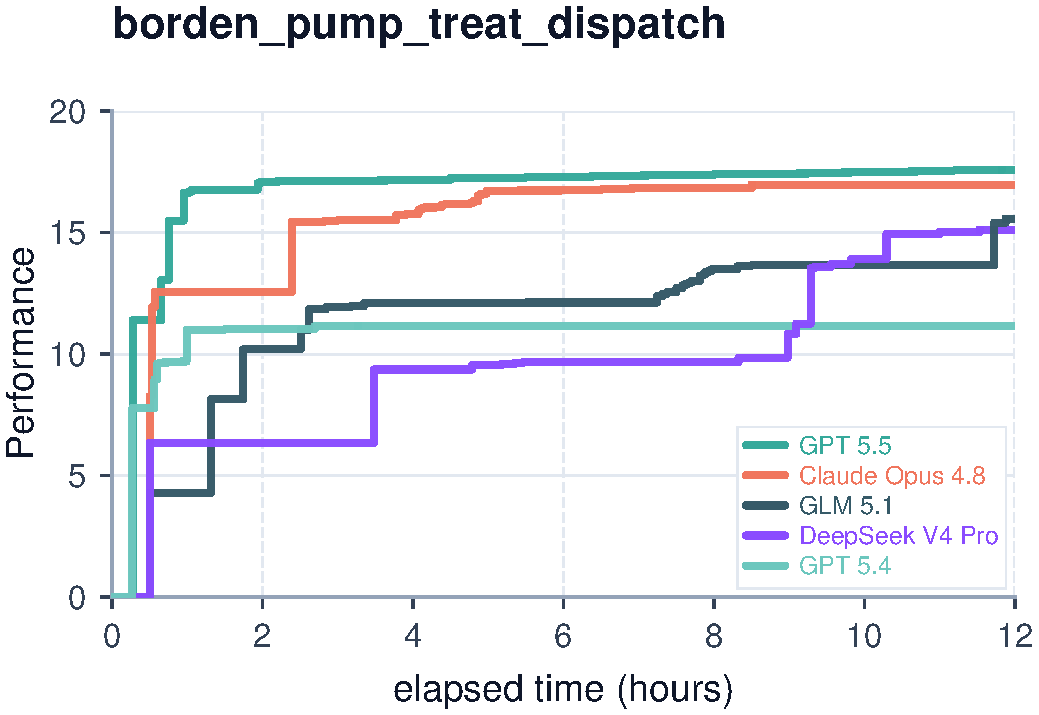
\includegraphics[width=\linewidth]{figures/curves/borden_emergency_modeling_time_performance.pdf}
\end{subfigure}
\hfill
\begin{subfigure}[b]{0.48\linewidth}
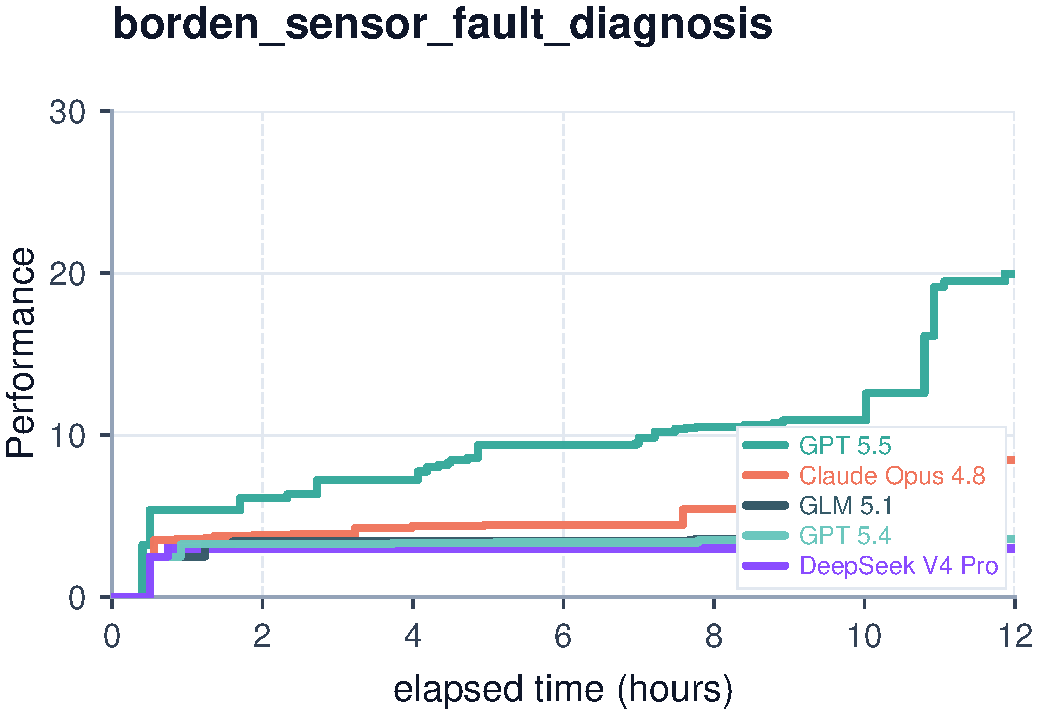
\includegraphics[width=\linewidth]{figures/curves/borden_qc_fault_diagnosis_time_performance.pdf}
\end{subfigure}
\vspace{0.5em}
\begin{subfigure}[b]{0.48\linewidth}
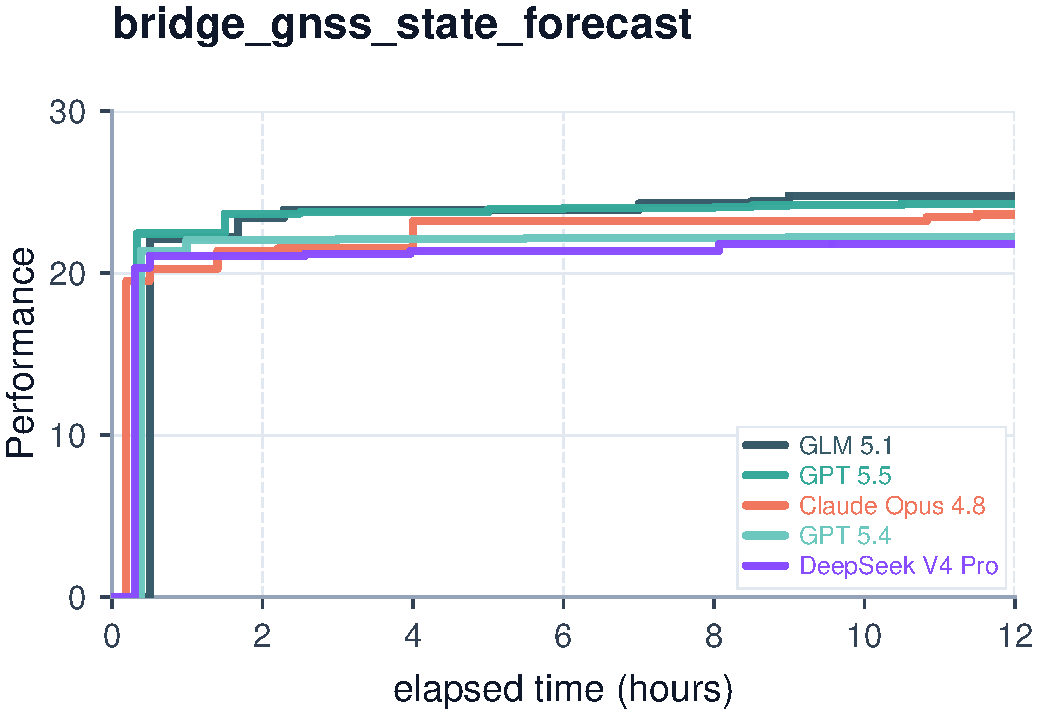
\includegraphics[width=\linewidth]{figures/curves/bridge_state_bench_time_performance.pdf}
\end{subfigure}
\hfill
\begin{subfigure}[b]{0.48\linewidth}
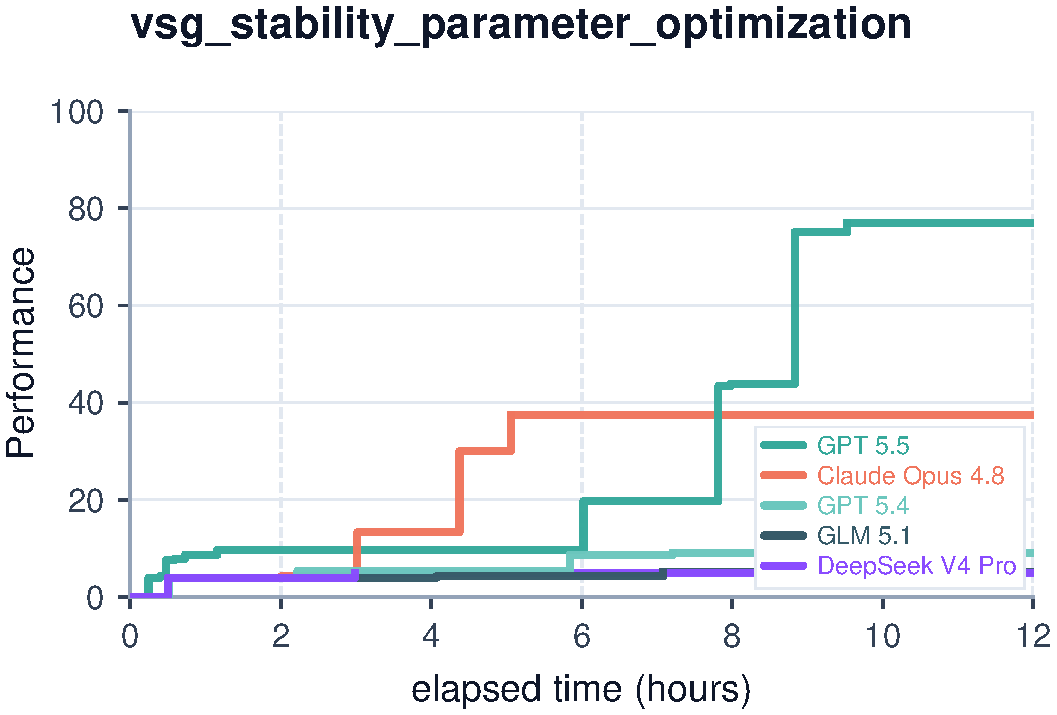
\includegraphics[width=\linewidth]{figures/curves/current_limited_vsg_bench_time_performance.pdf}
\end{subfigure}
\vspace{0.5em}
\begin{subfigure}[b]{0.48\linewidth}
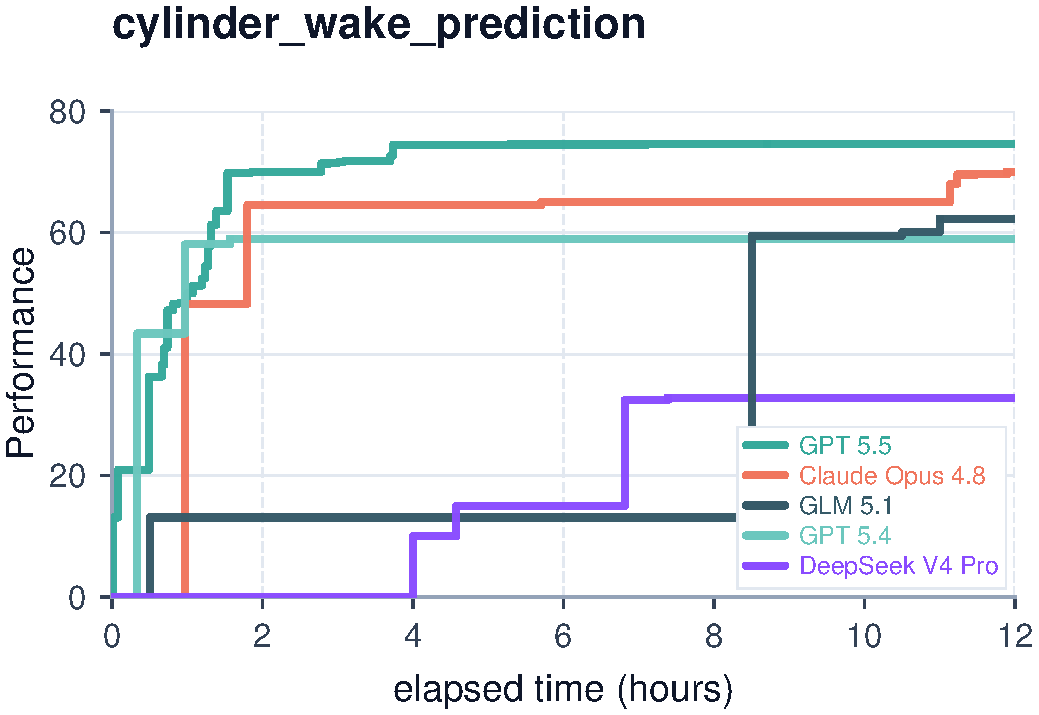
\includegraphics[width=\linewidth]{figures/curves/cylinder_wake_2d_time_performance.pdf}
\end{subfigure}
\hfill
\begin{subfigure}[b]{0.48\linewidth}
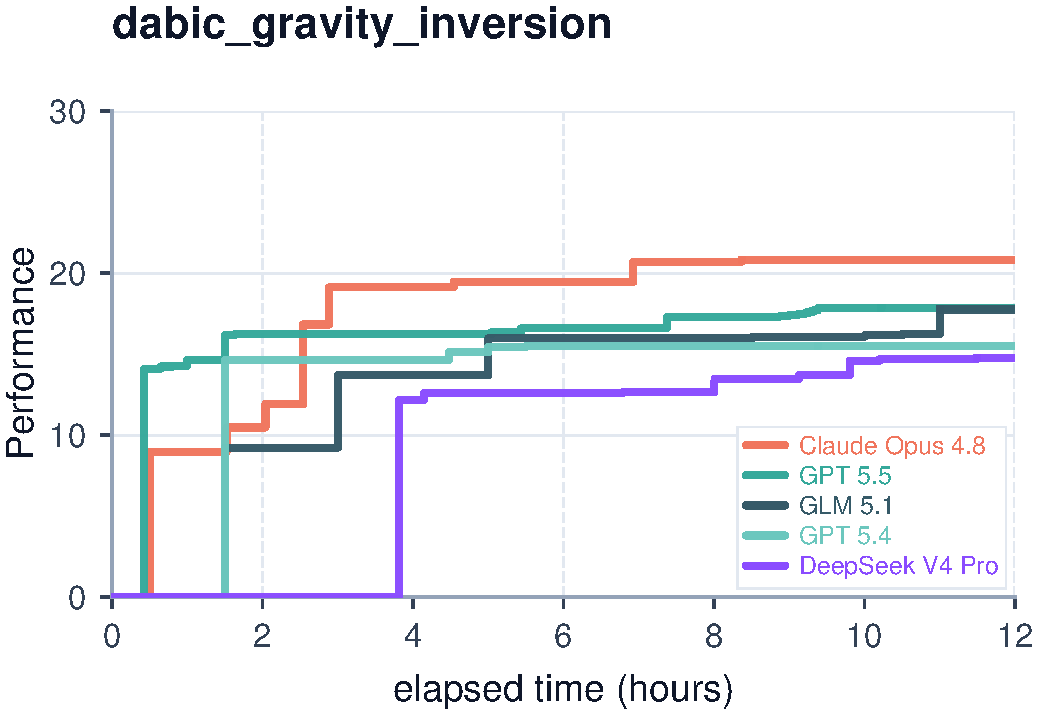
\includegraphics[width=\linewidth]{figures/curves/dabic_gravity_vinton_time_performance.pdf}
\end{subfigure}
\caption{Per-task learning curves: Scientific Computing \& ML (1/21).}
\label{fig:curves-all-1}
\end{figure}

\begin{figure}[p]
\centering
\begin{subfigure}[b]{0.48\linewidth}
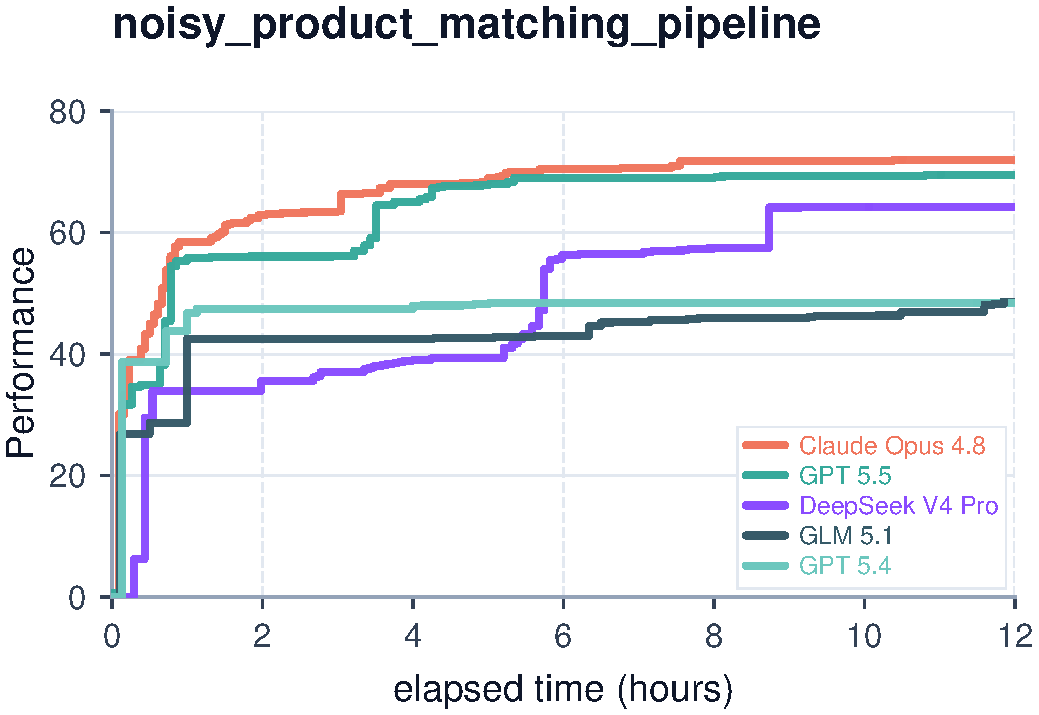
\includegraphics[width=\linewidth]{figures/curves/data_cleaning_pipeline_time_performance.pdf}
\end{subfigure}
\hfill
\begin{subfigure}[b]{0.48\linewidth}
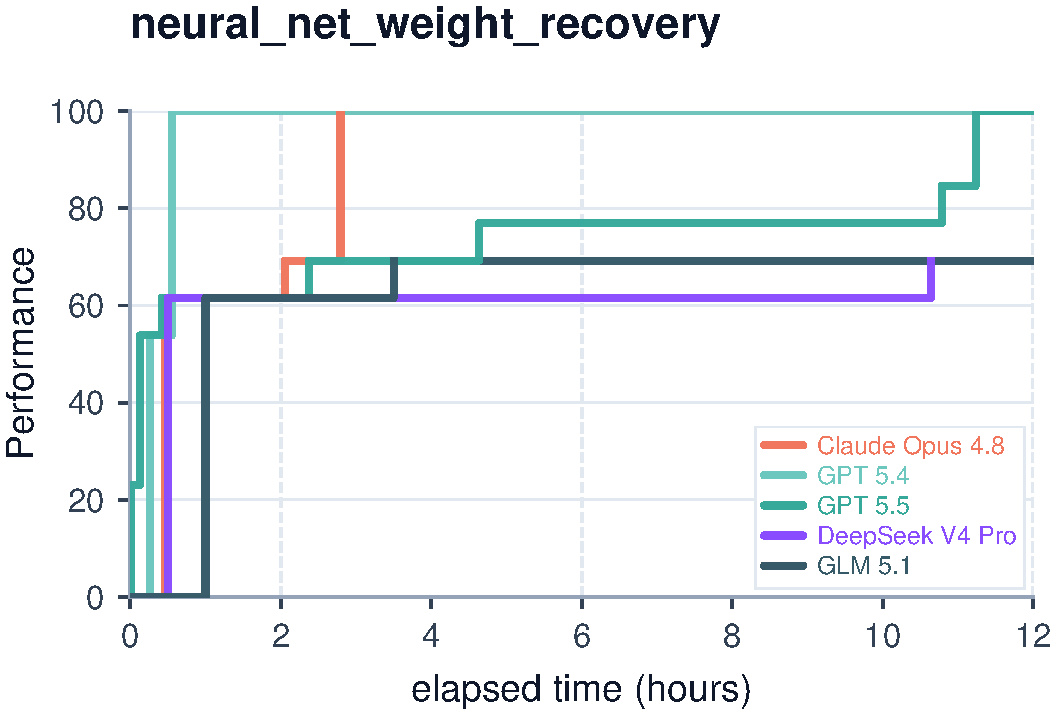
\includegraphics[width=\linewidth]{figures/curves/dropped_neural_net_time_performance.pdf}
\end{subfigure}
\vspace{0.5em}
\begin{subfigure}[b]{0.48\linewidth}
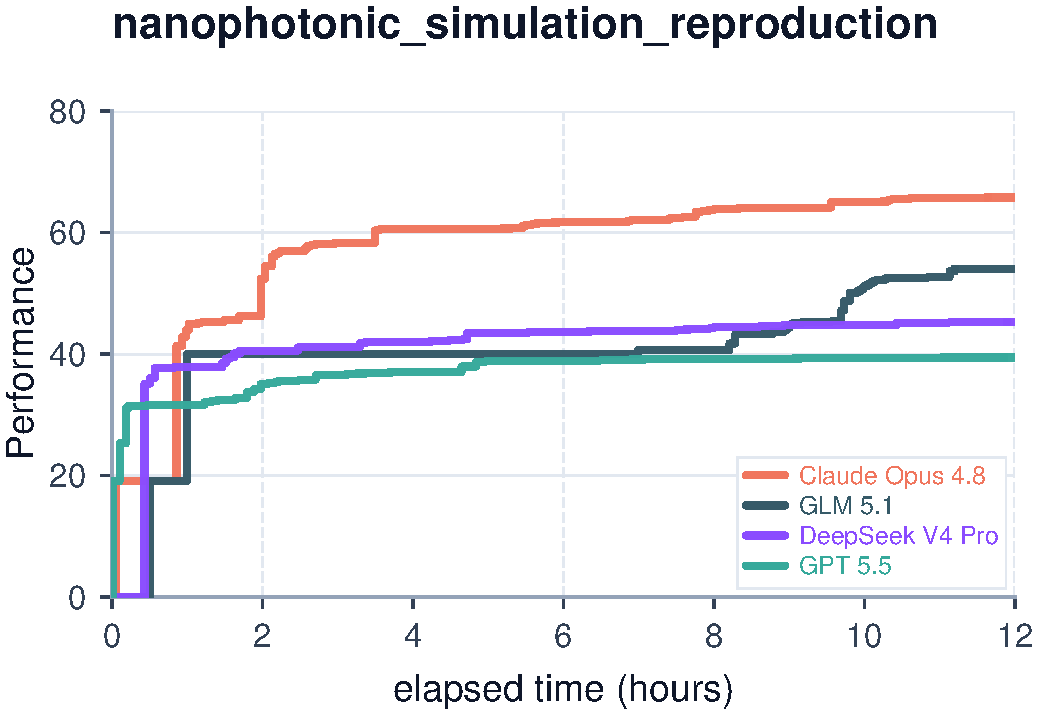
\includegraphics[width=\linewidth]{figures/curves/fast_multi_source_nanophotonic_sim_time_performance.pdf}
\end{subfigure}
\hfill
\begin{subfigure}[b]{0.48\linewidth}
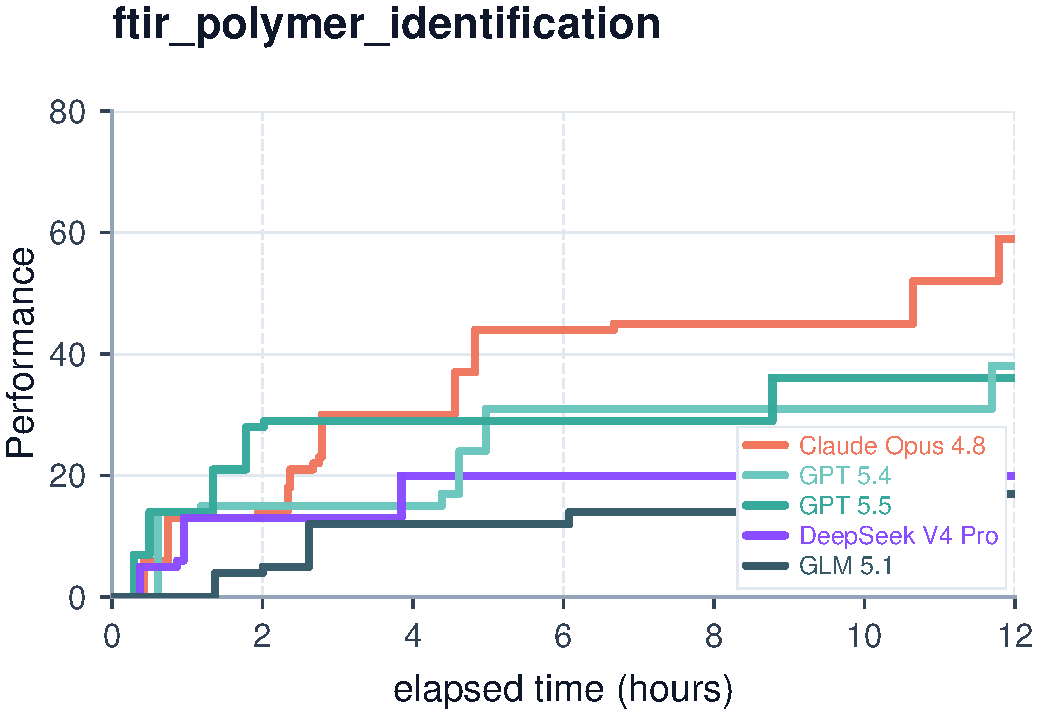
\includegraphics[width=\linewidth]{figures/curves/ftir_time_performance.pdf}
\end{subfigure}
\vspace{0.5em}
\begin{subfigure}[b]{0.48\linewidth}
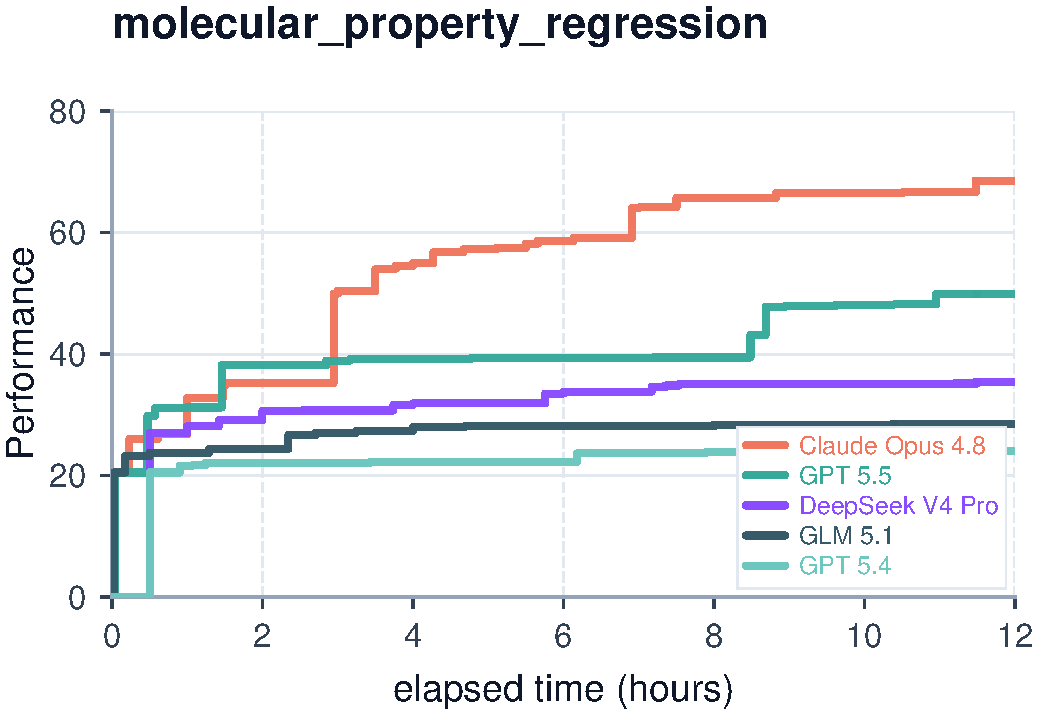
\includegraphics[width=\linewidth]{figures/curves/gnn_molecular_property_regression_time_performance.pdf}
\end{subfigure}
\hfill
\begin{subfigure}[b]{0.48\linewidth}
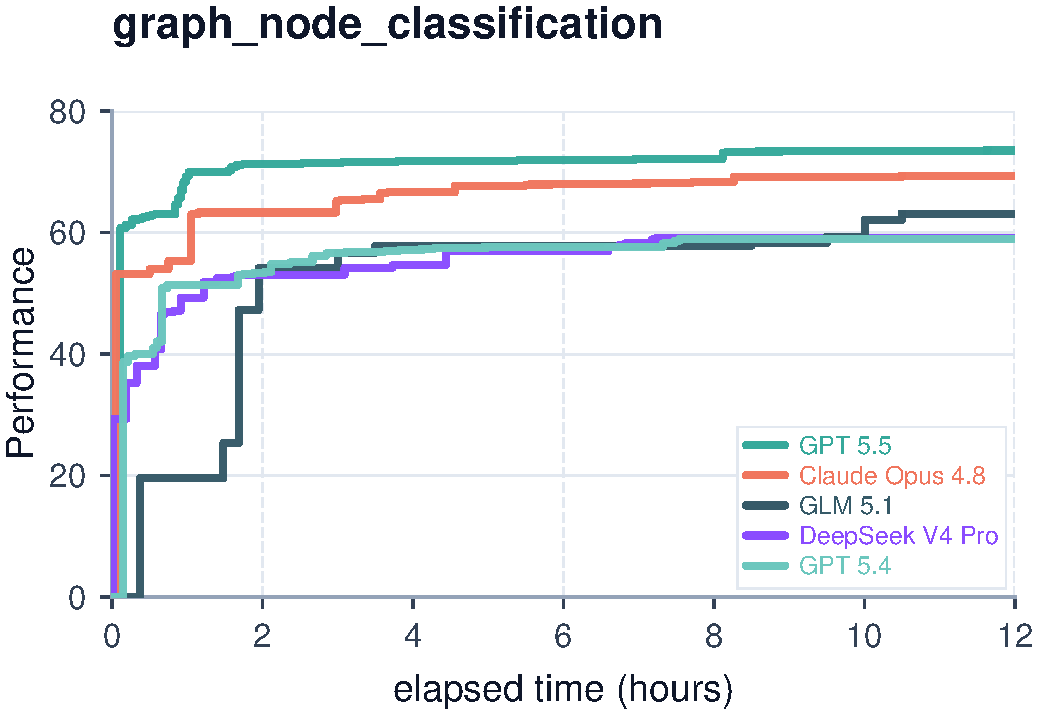
\includegraphics[width=\linewidth]{figures/curves/graph_node_classification_time_performance.pdf}
\end{subfigure}
\caption{Per-task learning curves: Scientific Computing \& ML cont. (2/21).}
\label{fig:curves-all-2}
\end{figure}

\begin{figure}[p]
\centering
\begin{subfigure}[b]{0.48\linewidth}
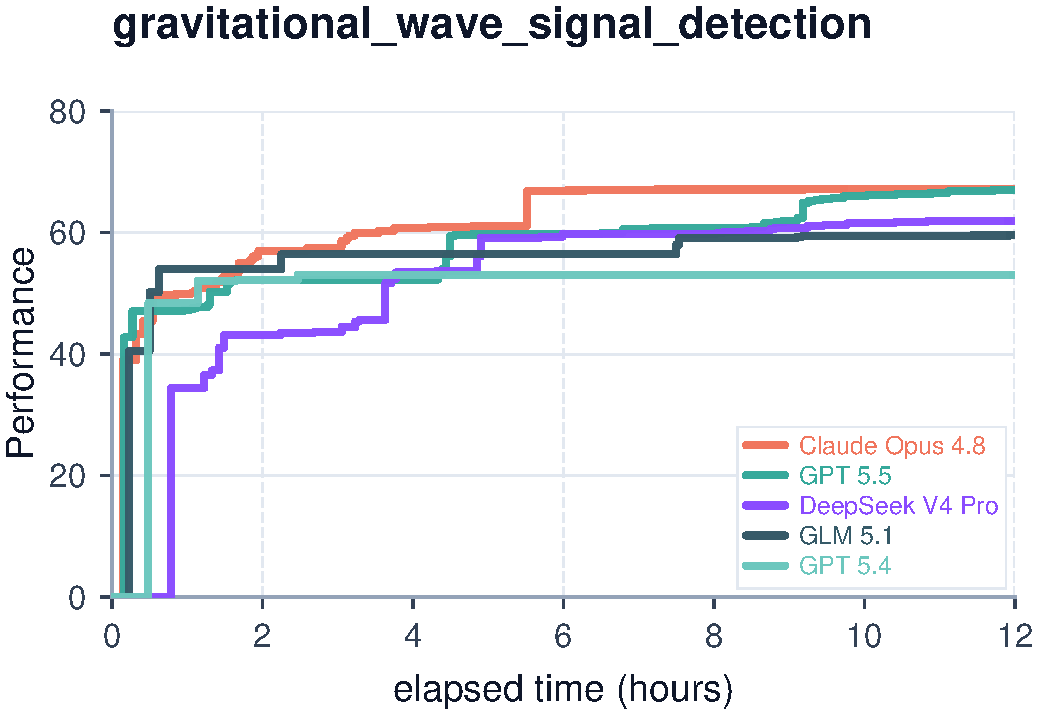
\includegraphics[width=\linewidth]{figures/curves/gravitational_wave_time_performance.pdf}
\end{subfigure}
\hfill
\begin{subfigure}[b]{0.48\linewidth}
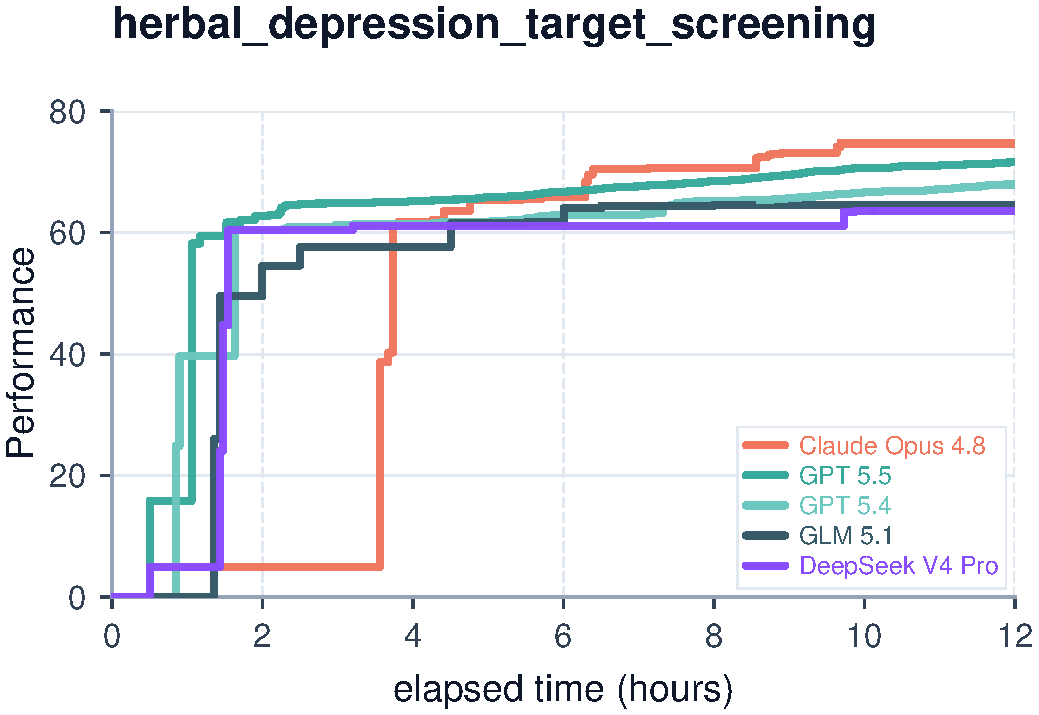
\includegraphics[width=\linewidth]{figures/curves/herbal_depression_targets_time_performance.pdf}
\end{subfigure}
\vspace{0.5em}
\begin{subfigure}[b]{0.48\linewidth}
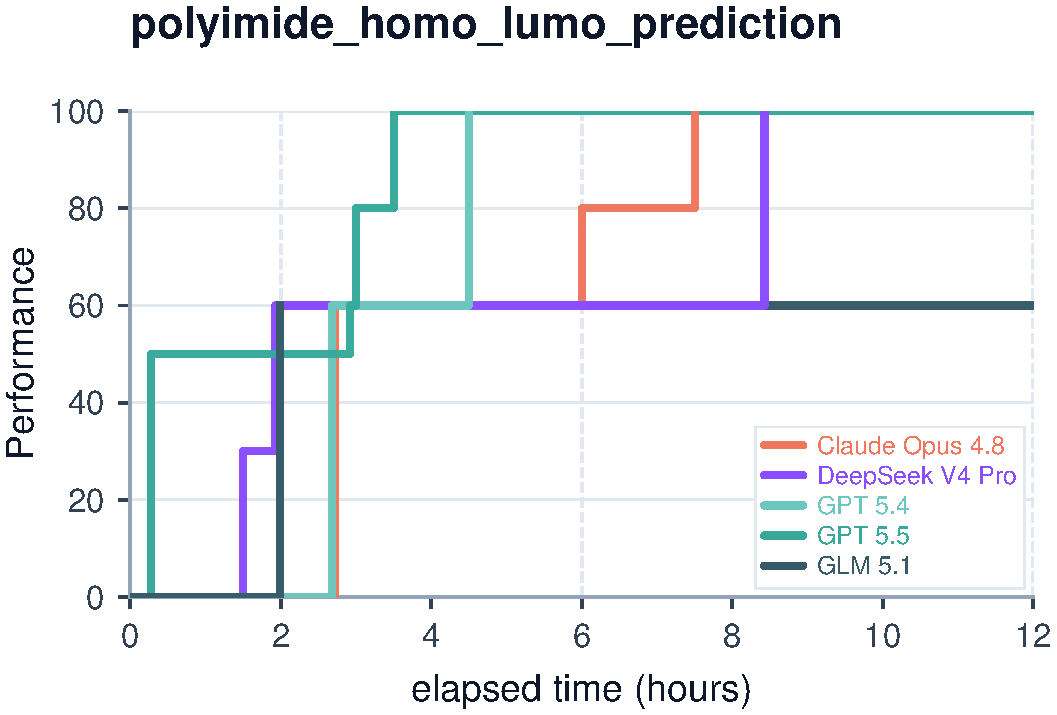
\includegraphics[width=\linewidth]{figures/curves/homo_lumo_time_performance.pdf}
\end{subfigure}
\hfill
\begin{subfigure}[b]{0.48\linewidth}
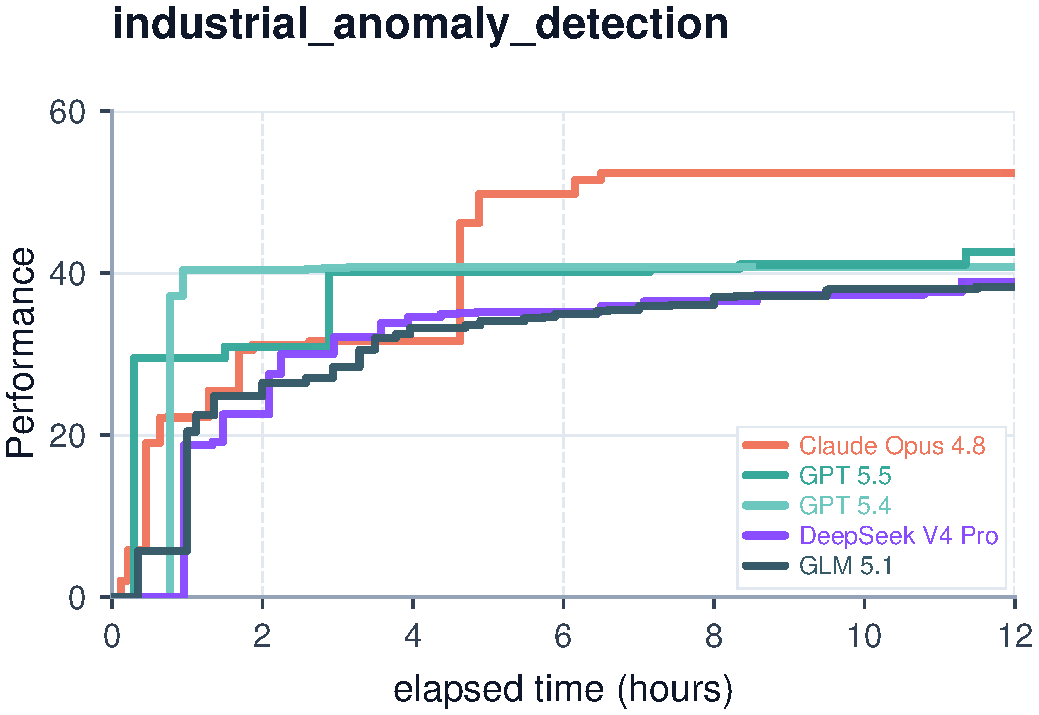
\includegraphics[width=\linewidth]{figures/curves/industrial_anomaly_detection_time_performance.pdf}
\end{subfigure}
\vspace{0.5em}
\begin{subfigure}[b]{0.48\linewidth}
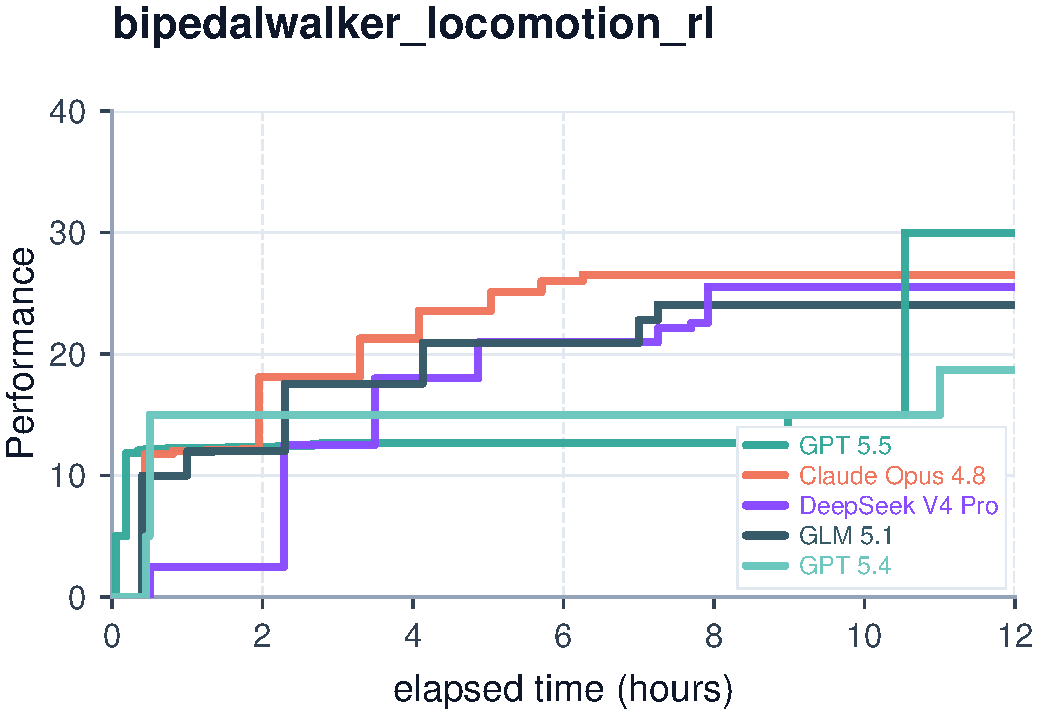
\includegraphics[width=\linewidth]{figures/curves/loco_rl_locomotion_time_performance.pdf}
\end{subfigure}
\hfill
\begin{subfigure}[b]{0.48\linewidth}
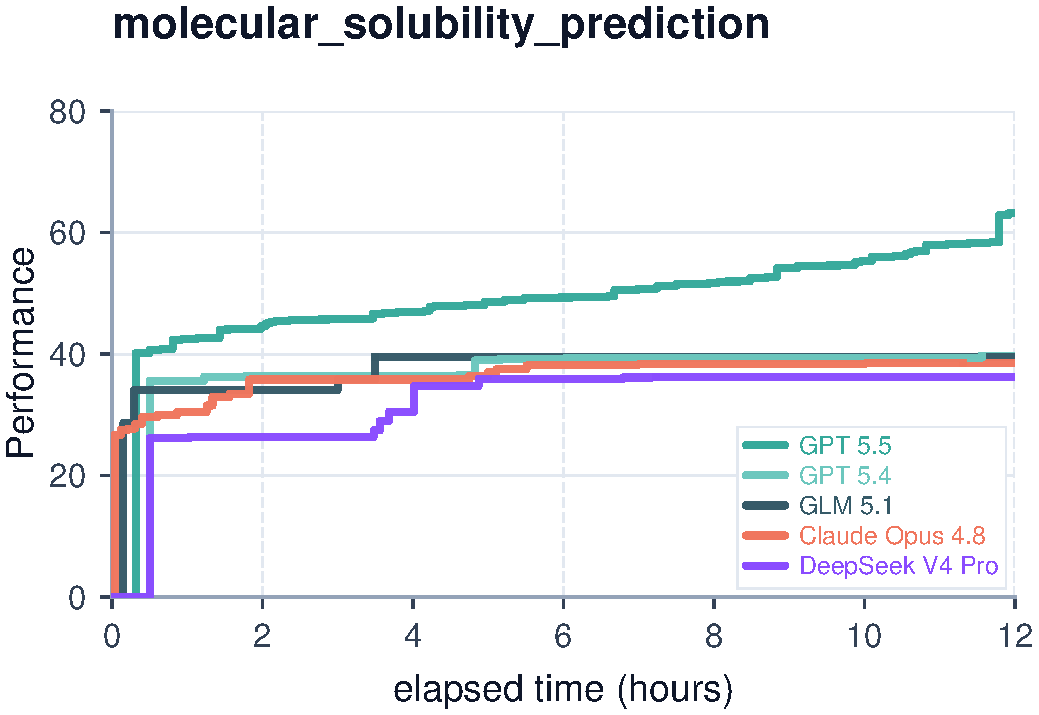
\includegraphics[width=\linewidth]{figures/curves/molecular_solubility_prediction_time_performance.pdf}
\end{subfigure}
\caption{Per-task learning curves: Scientific Computing \& ML cont. (3/21).}
\label{fig:curves-all-3}
\end{figure}

\begin{figure}[p]
\centering
\begin{subfigure}[b]{0.48\linewidth}
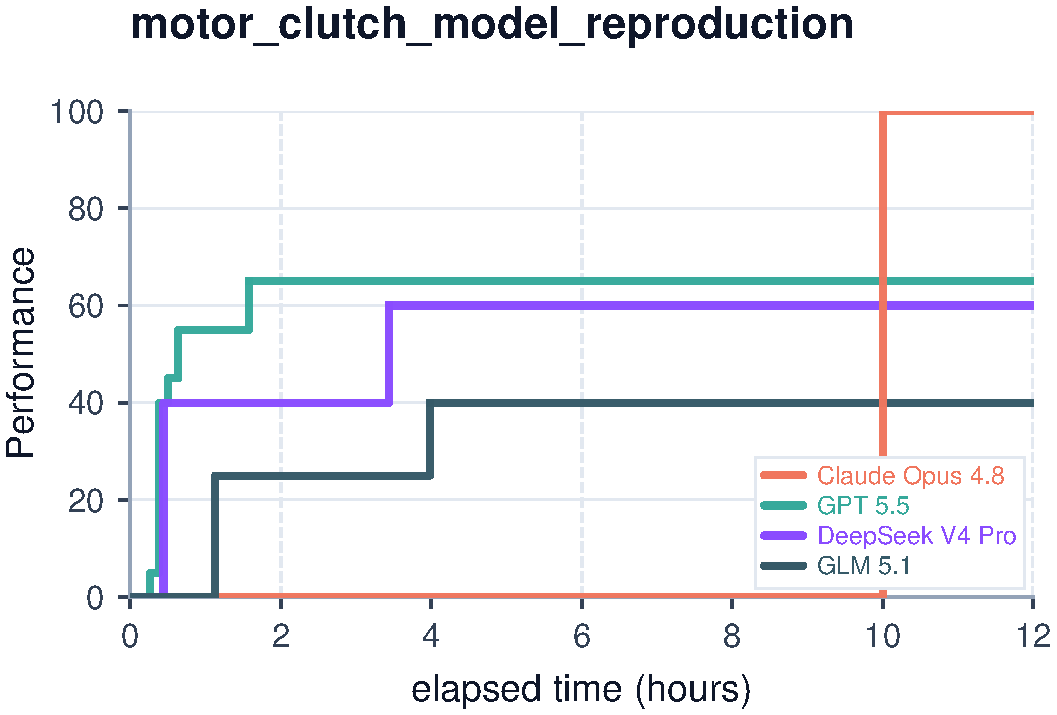
\includegraphics[width=\linewidth]{figures/curves/motor_clutch_repro_public_refs_strong_blind_slow_time_performance.pdf}
\end{subfigure}
\hfill
\begin{subfigure}[b]{0.48\linewidth}
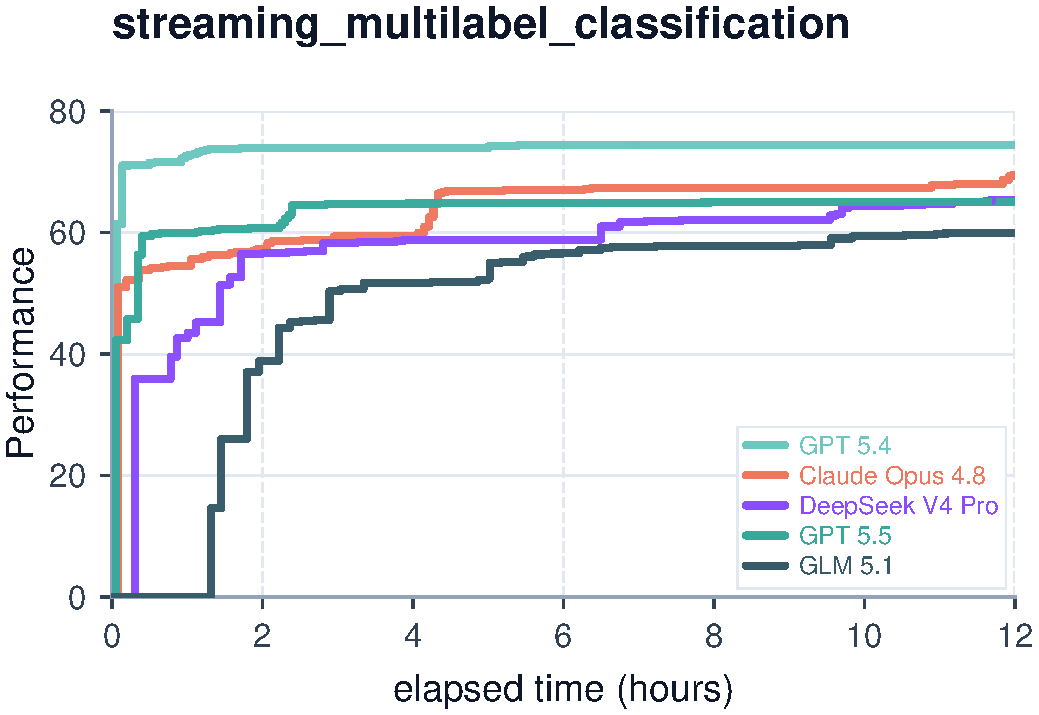
\includegraphics[width=\linewidth]{figures/curves/multi_label_classification_time_performance.pdf}
\end{subfigure}
\vspace{0.5em}
\begin{subfigure}[b]{0.48\linewidth}
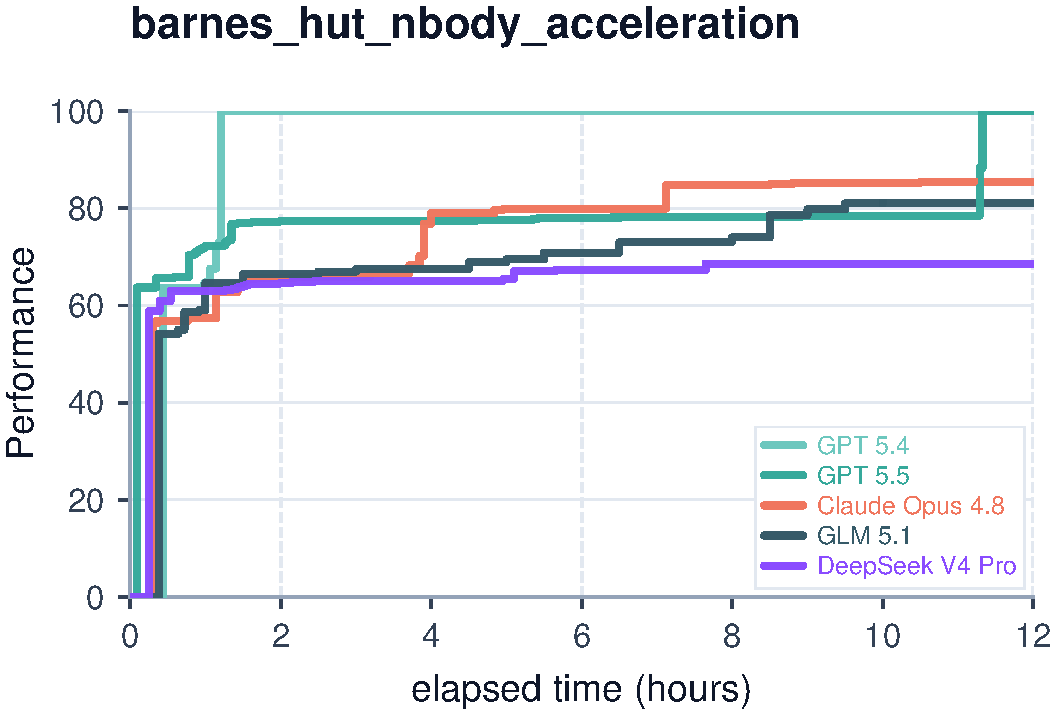
\includegraphics[width=\linewidth]{figures/curves/n_body_simulation_acceleration_time_performance.pdf}
\end{subfigure}
\hfill
\begin{subfigure}[b]{0.48\linewidth}
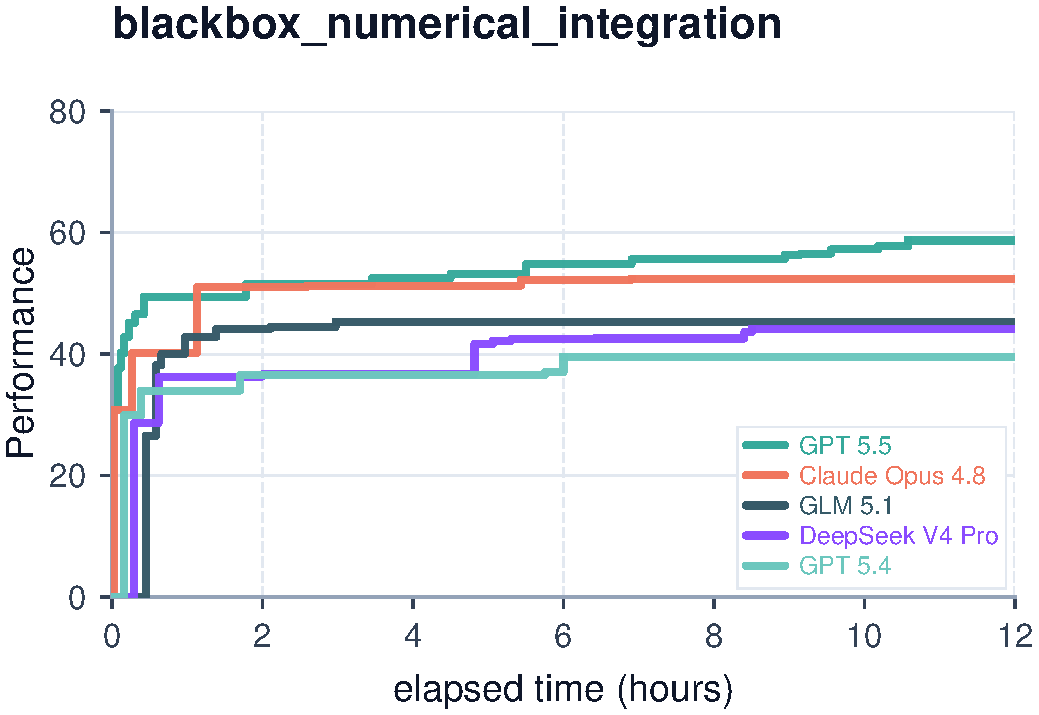
\includegraphics[width=\linewidth]{figures/curves/numerical_integration_accuracy_optimization_time_performance.pdf}
\end{subfigure}
\vspace{0.5em}
\begin{subfigure}[b]{0.48\linewidth}
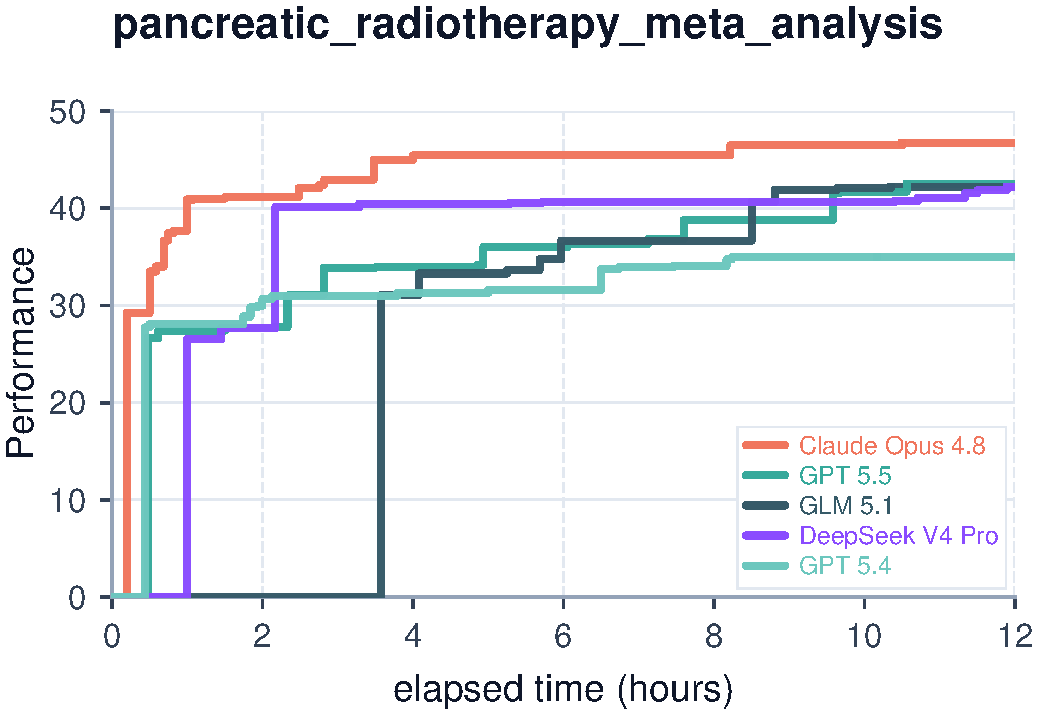
\includegraphics[width=\linewidth]{figures/curves/pancreatic_radiotherapy_meta_analysis_time_performance.pdf}
\end{subfigure}
\hfill
\begin{subfigure}[b]{0.48\linewidth}
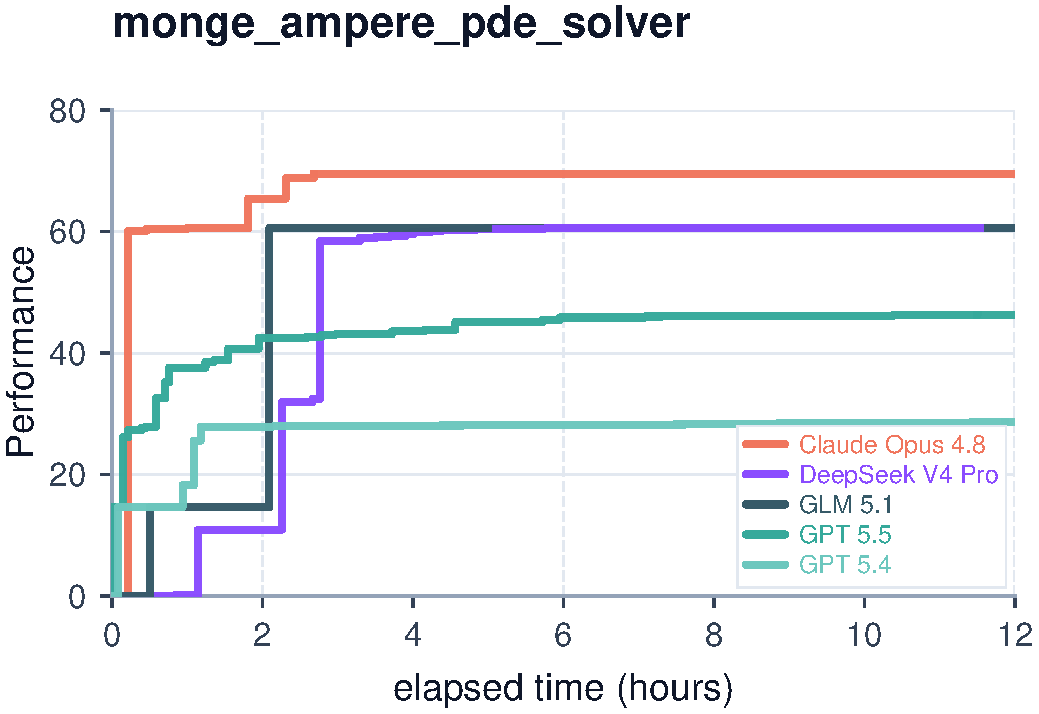
\includegraphics[width=\linewidth]{figures/curves/pde_solver_optimization_time_performance.pdf}
\end{subfigure}
\caption{Per-task learning curves: Scientific Computing \& ML cont. (4/21).}
\label{fig:curves-all-4}
\end{figure}

\begin{figure}[p]
\centering
\begin{subfigure}[b]{0.48\linewidth}
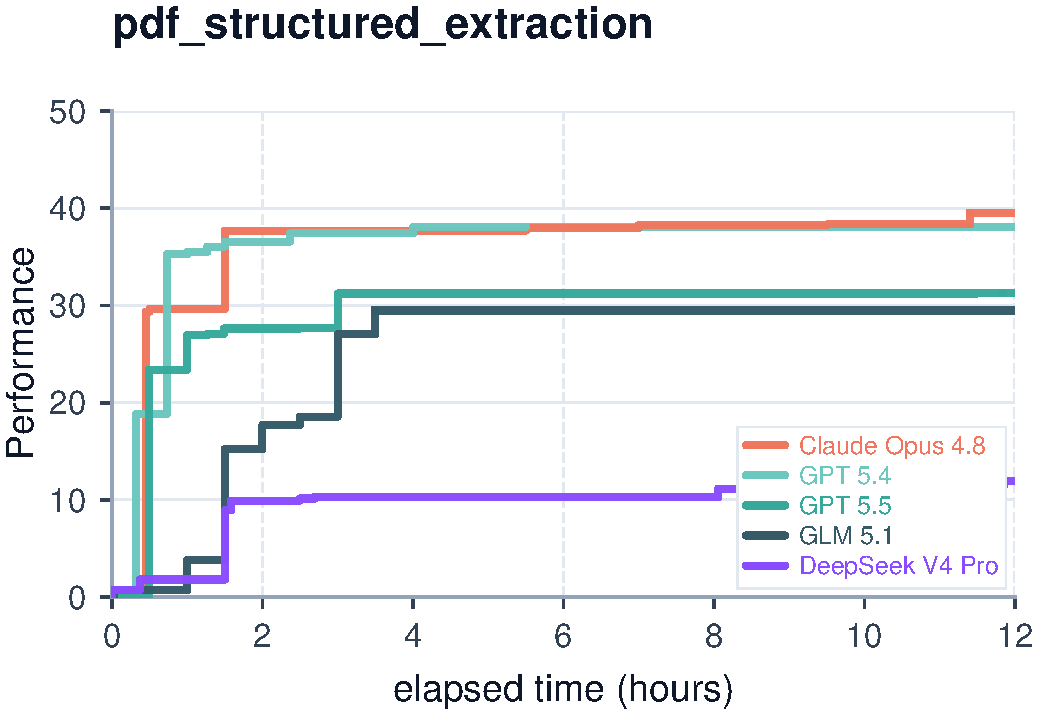
\includegraphics[width=\linewidth]{figures/curves/pdf_data_extraction_pipeline_time_performance.pdf}
\end{subfigure}
\hfill
\begin{subfigure}[b]{0.48\linewidth}
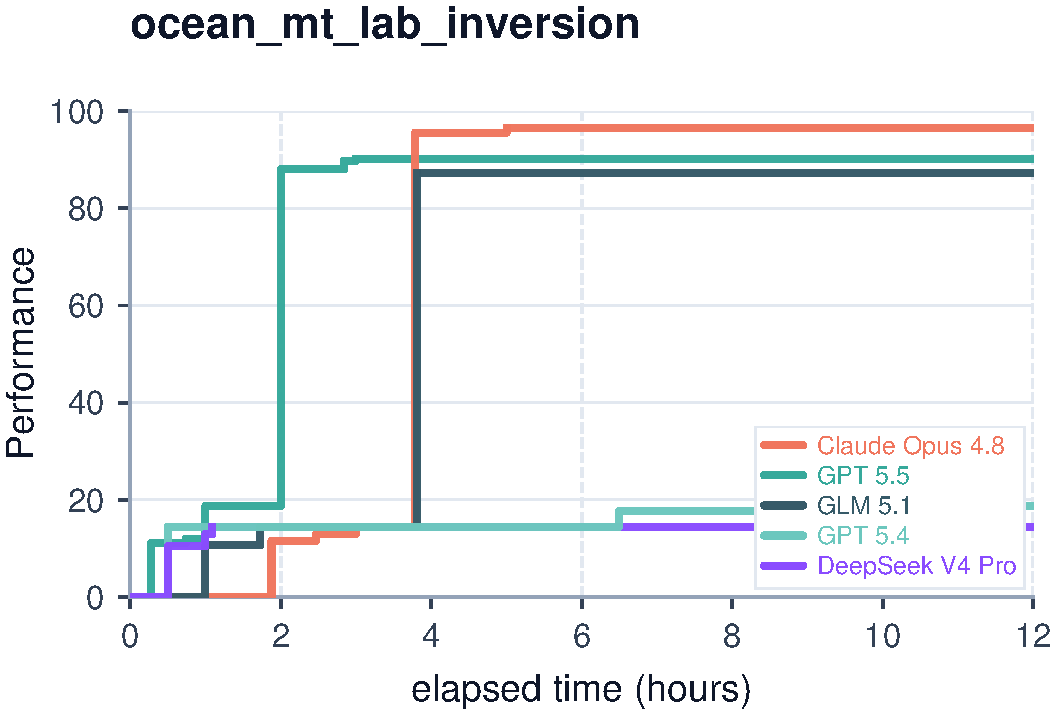
\includegraphics[width=\linewidth]{figures/curves/pseudo2d_mt_lab_inversion_time_performance.pdf}
\end{subfigure}
\vspace{0.5em}
\begin{subfigure}[b]{0.48\linewidth}
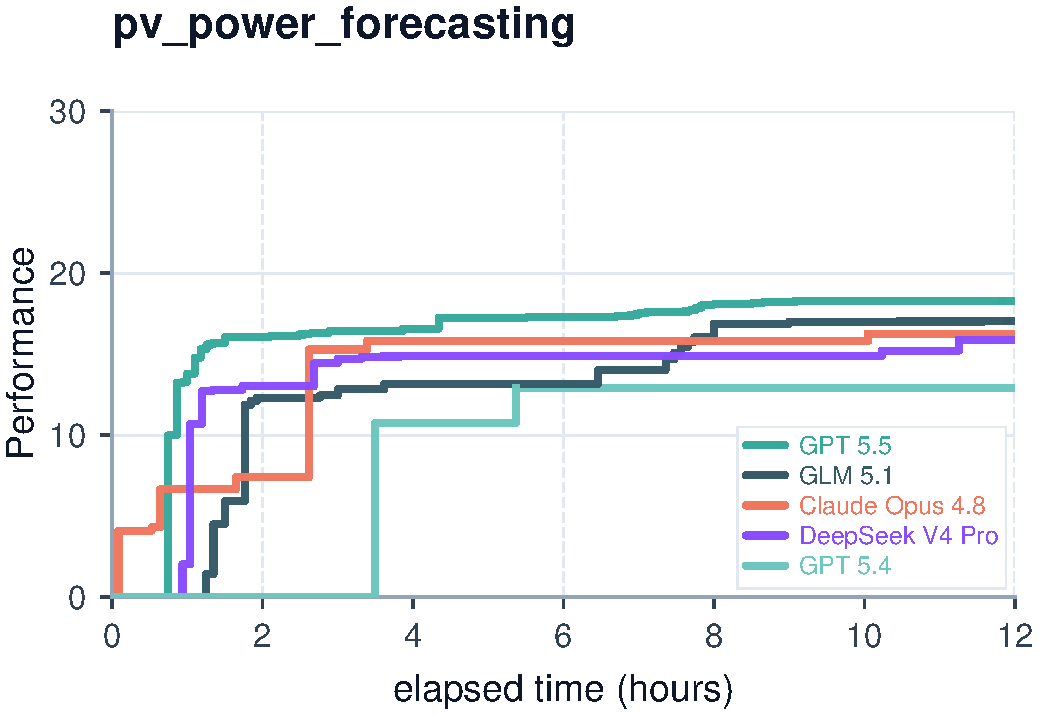
\includegraphics[width=\linewidth]{figures/curves/pv_power_forecasting_time_performance.pdf}
\end{subfigure}
\hfill
\begin{subfigure}[b]{0.48\linewidth}
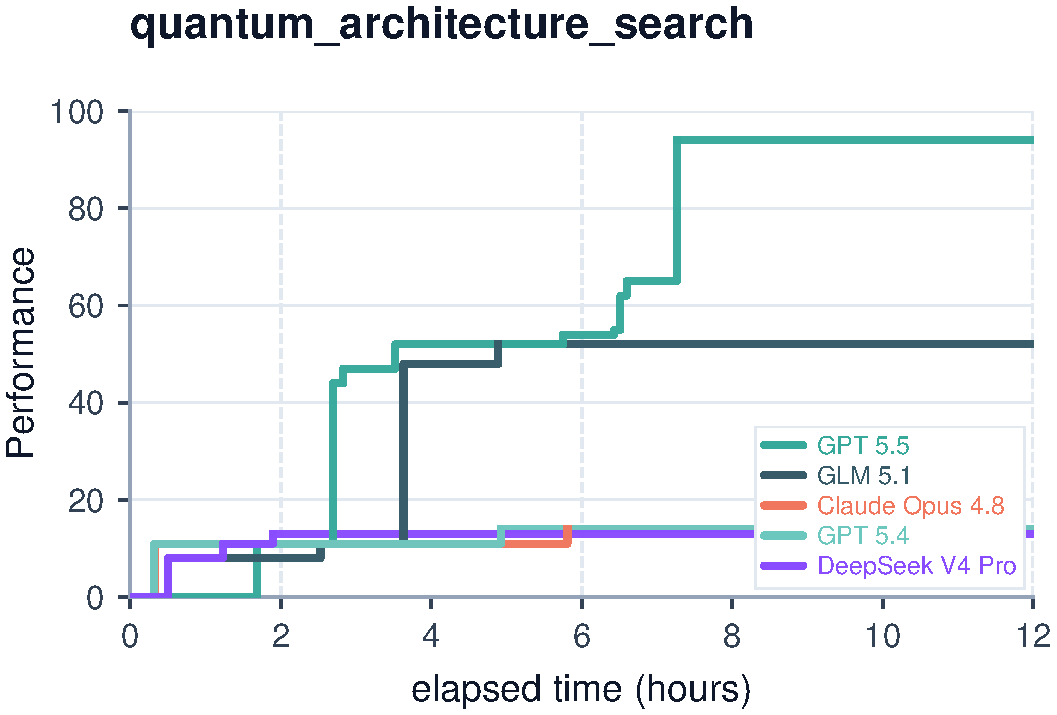
\includegraphics[width=\linewidth]{figures/curves/qastask_time_performance.pdf}
\end{subfigure}
\vspace{0.5em}
\begin{subfigure}[b]{0.48\linewidth}
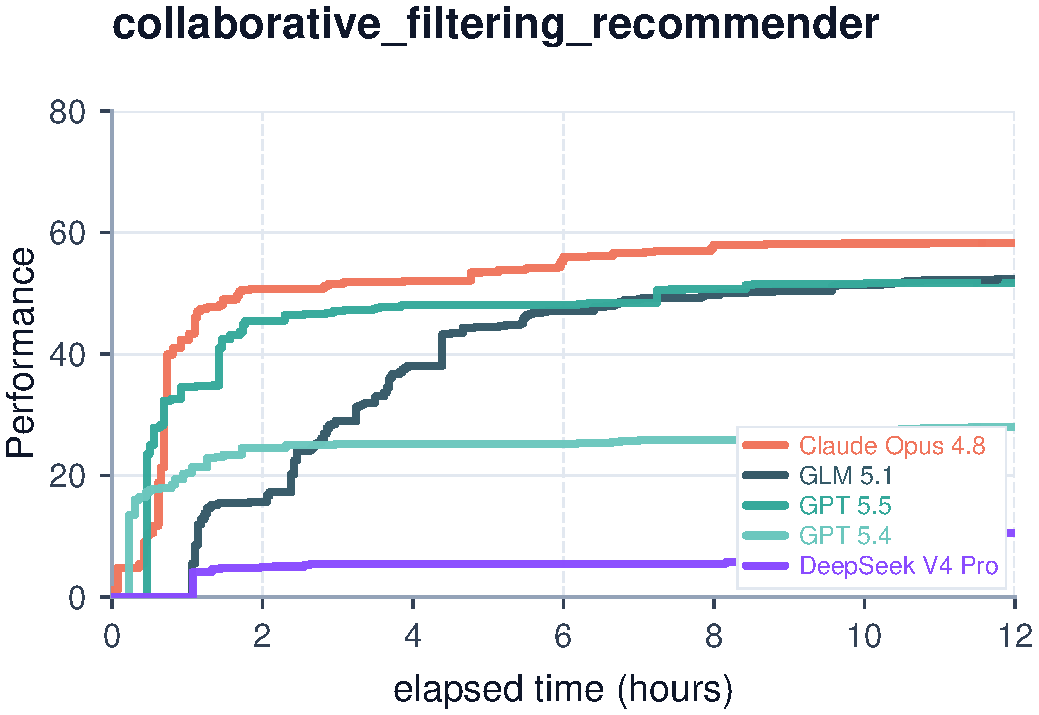
\includegraphics[width=\linewidth]{figures/curves/recommender_system_collaborative_filtering_time_performance.pdf}
\end{subfigure}
\hfill
\begin{subfigure}[b]{0.48\linewidth}
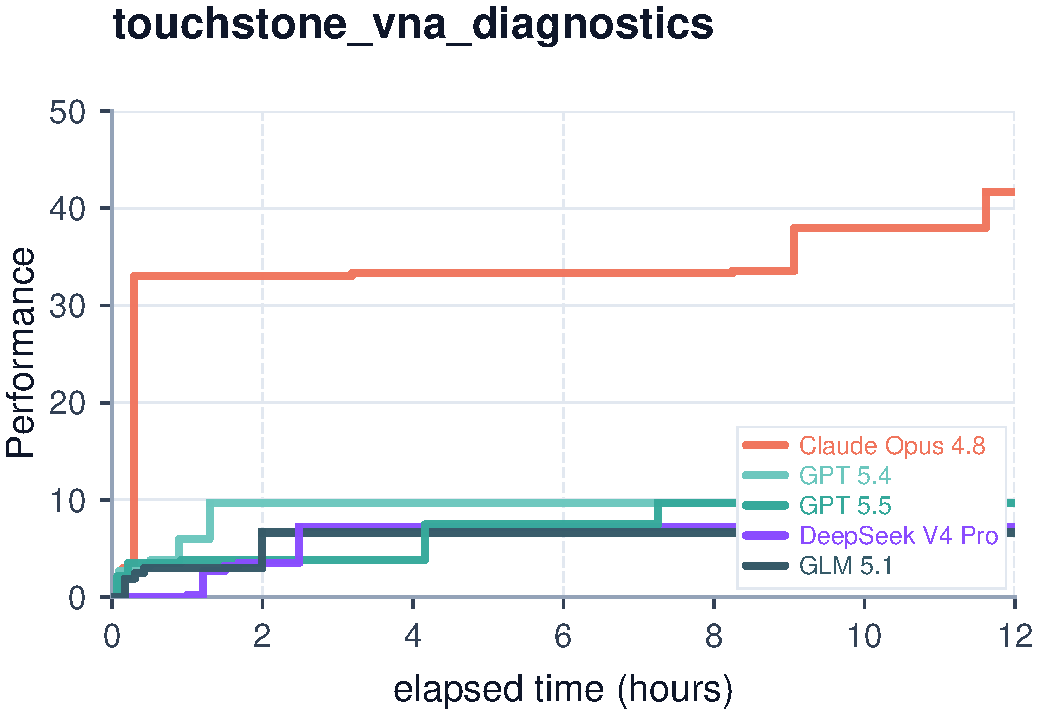
\includegraphics[width=\linewidth]{figures/curves/rf_touchstone_vna_diagnostics_time_performance.pdf}
\end{subfigure}
\caption{Per-task learning curves: Scientific Computing \& ML cont. (5/21).}
\label{fig:curves-all-5}
\end{figure}

\begin{figure}[p]
\centering
\begin{subfigure}[b]{0.48\linewidth}
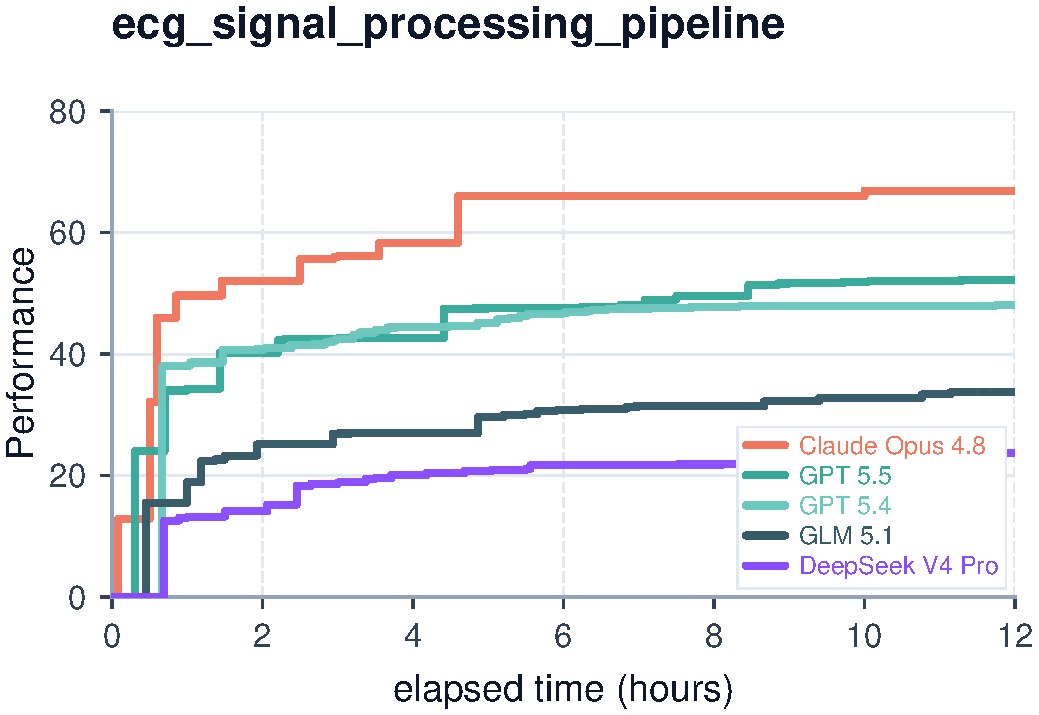
\includegraphics[width=\linewidth]{figures/curves/signal_processing_pipeline_time_performance.pdf}
\end{subfigure}
\hfill
\begin{subfigure}[b]{0.48\linewidth}
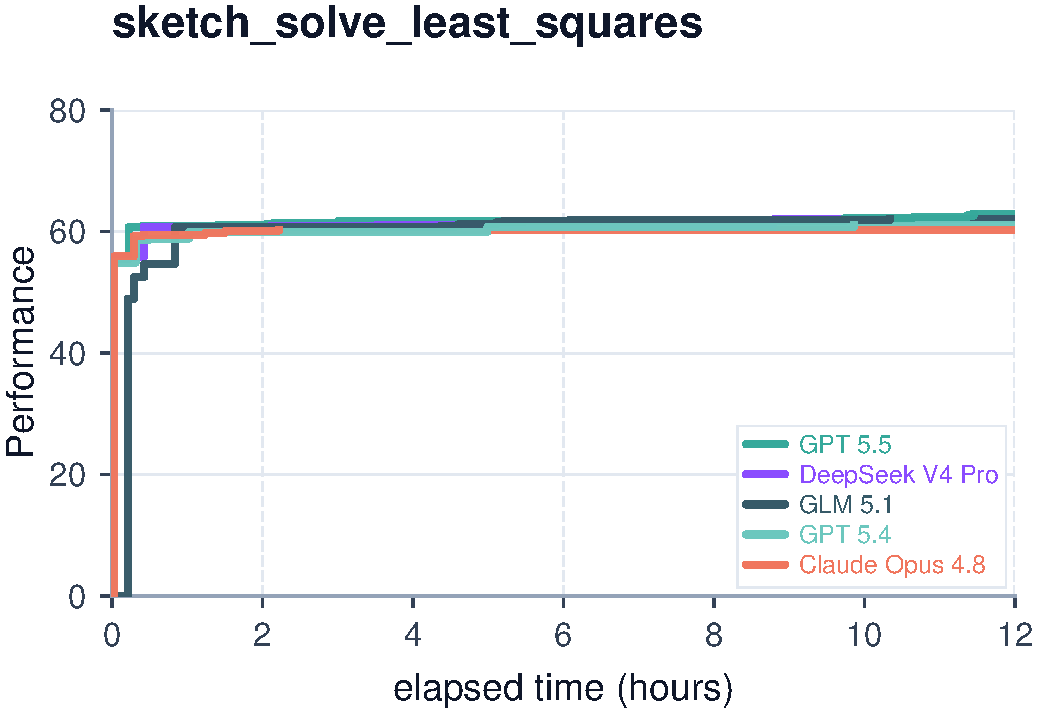
\includegraphics[width=\linewidth]{figures/curves/sketch_n_solve_benchmark_time_performance.pdf}
\end{subfigure}
\vspace{0.5em}
\begin{subfigure}[b]{0.48\linewidth}
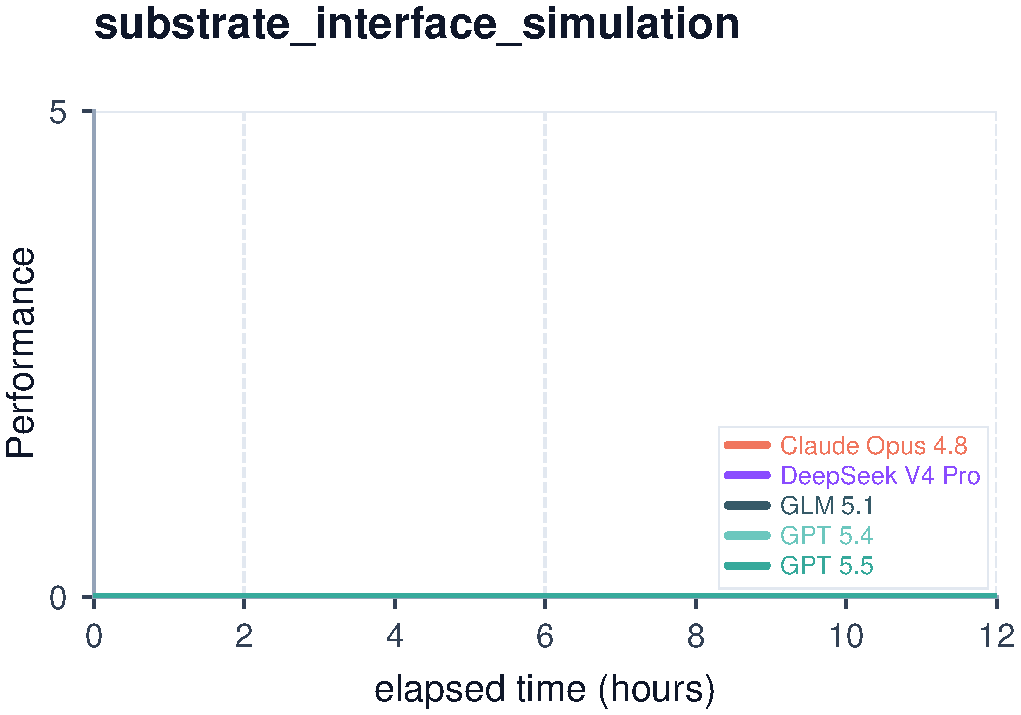
\includegraphics[width=\linewidth]{figures/curves/substrate_interface_response_prelim_time_performance.pdf}
\end{subfigure}
\hfill
\begin{subfigure}[b]{0.48\linewidth}
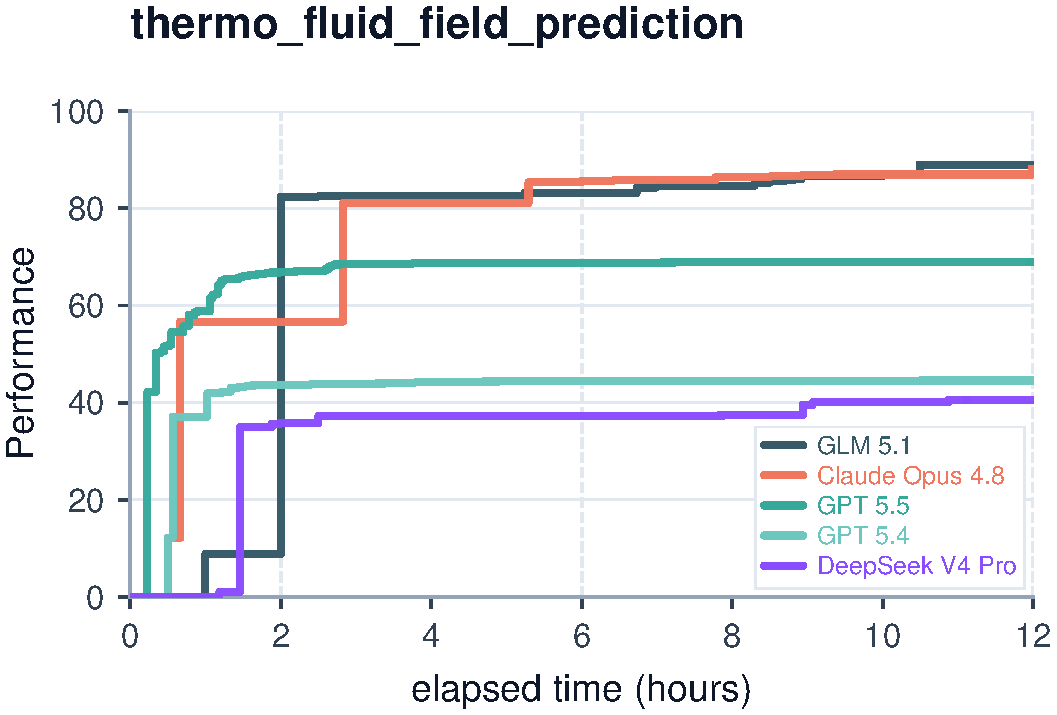
\includegraphics[width=\linewidth]{figures/curves/thermo_fluid_coupling_field_prediction_time_performance.pdf}
\end{subfigure}
\vspace{0.5em}
\begin{subfigure}[b]{0.48\linewidth}
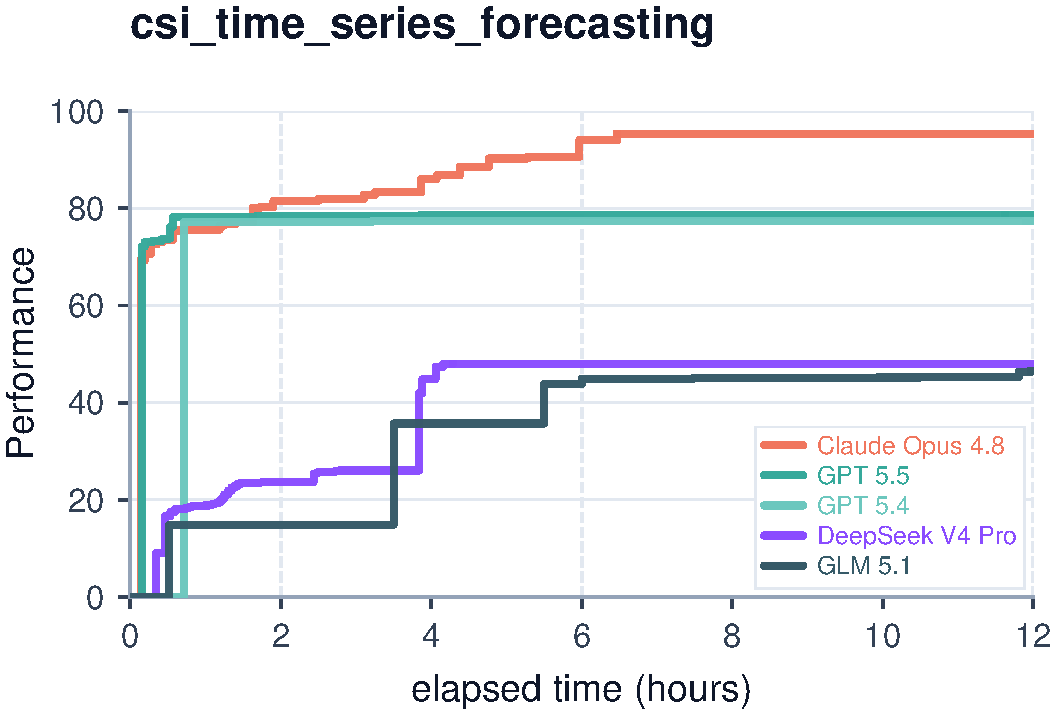
\includegraphics[width=\linewidth]{figures/curves/time_series_forecasting_cpu_time_performance.pdf}
\end{subfigure}
\hfill
\begin{subfigure}[b]{0.48\linewidth}
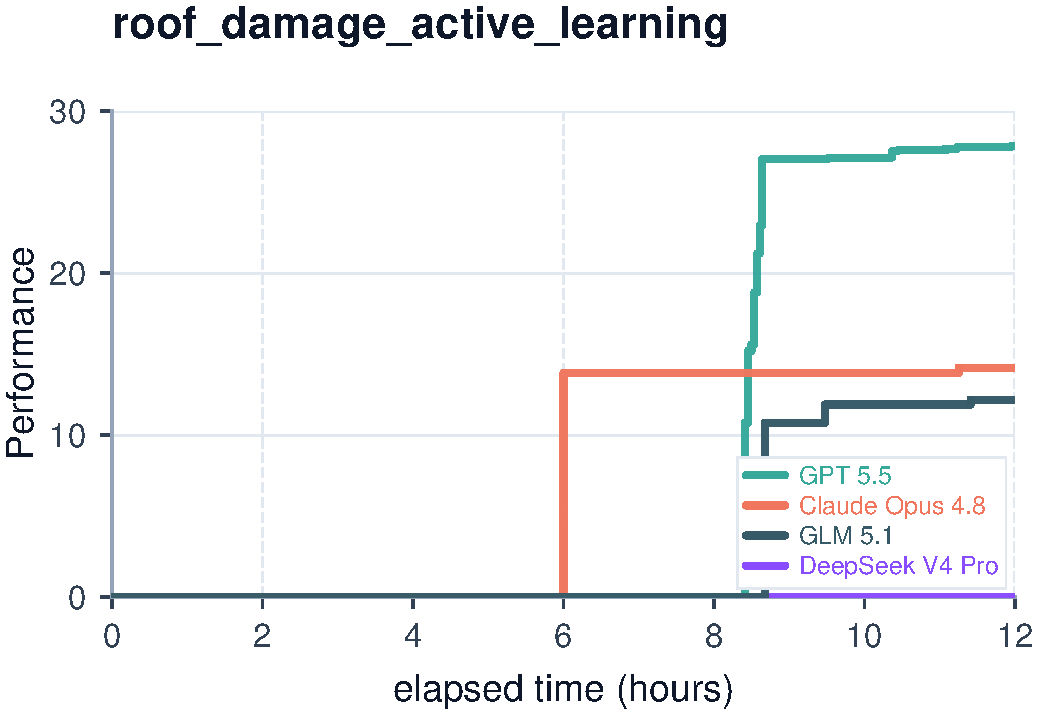
\includegraphics[width=\linewidth]{figures/curves/village_roof_al_time_performance.pdf}
\end{subfigure}
\caption{Per-task learning curves: Scientific Computing \& ML cont. (6/21).}
\label{fig:curves-all-6}
\end{figure}

\begin{figure}[p]
\centering
\begin{subfigure}[b]{0.48\linewidth}
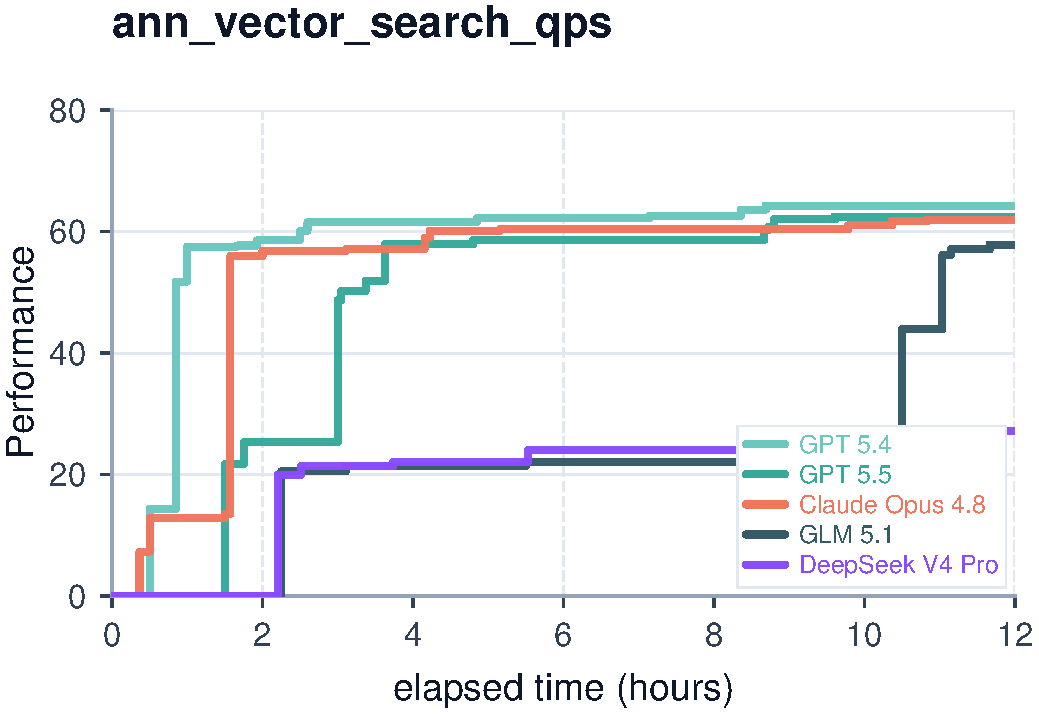
\includegraphics[width=\linewidth]{figures/curves/ann_search_time_performance.pdf}
\end{subfigure}
\hfill
\begin{subfigure}[b]{0.48\linewidth}
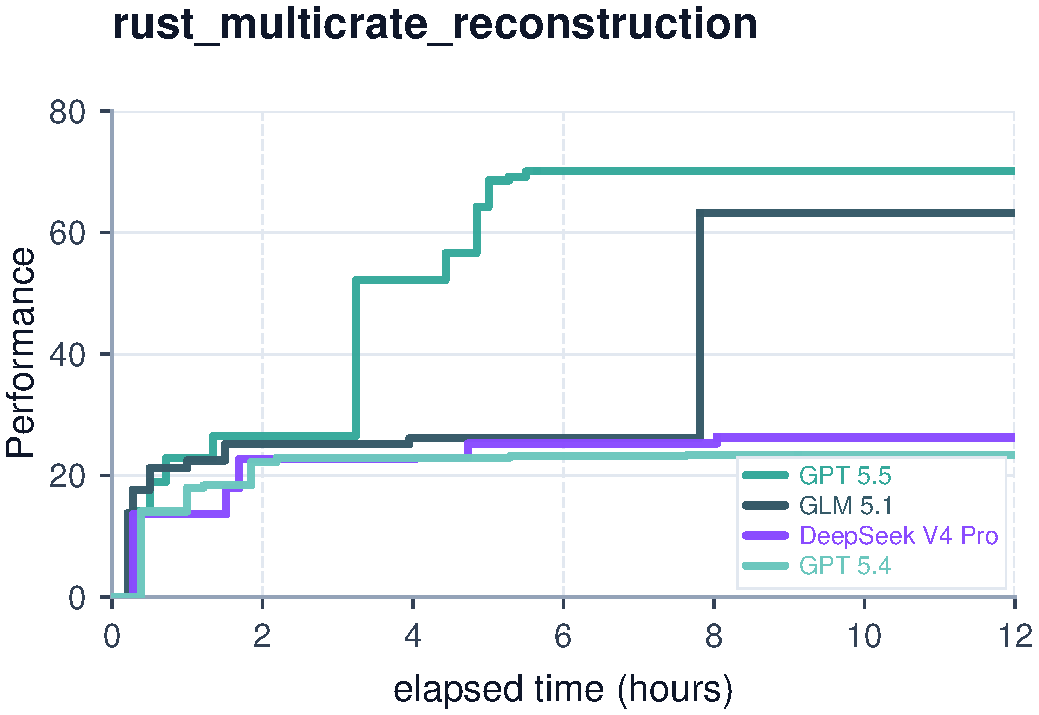
\includegraphics[width=\linewidth]{figures/curves/cas_rust_benchmark_time_performance.pdf}
\end{subfigure}
\vspace{0.5em}
\begin{subfigure}[b]{0.48\linewidth}
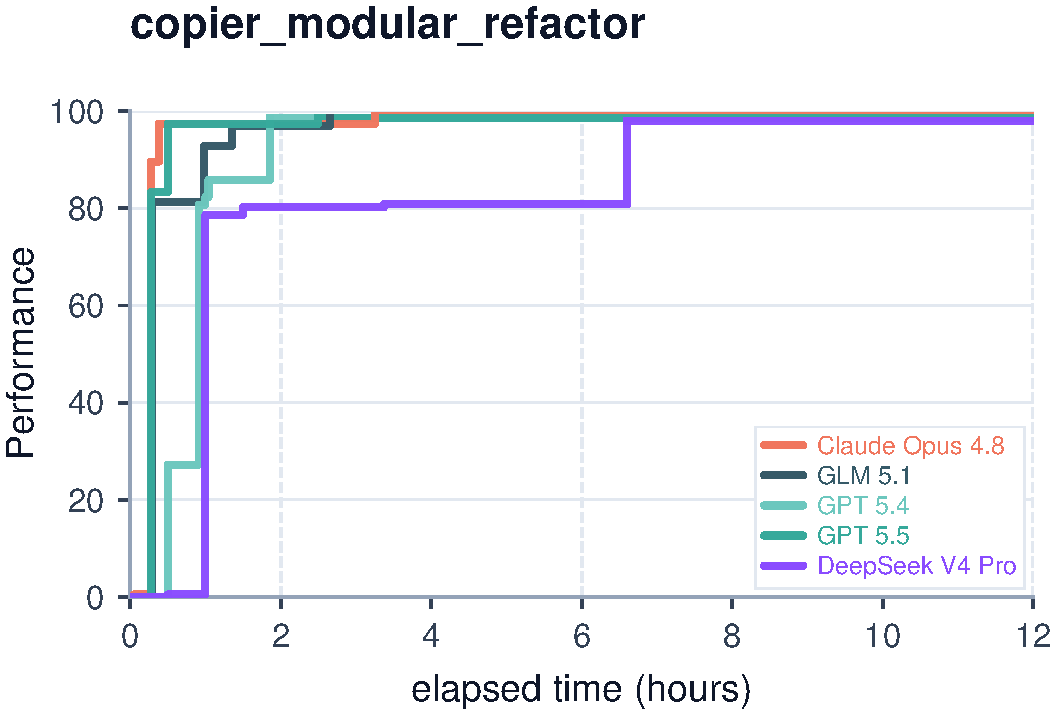
\includegraphics[width=\linewidth]{figures/curves/copier_modular_time_performance.pdf}
\end{subfigure}
\hfill
\begin{subfigure}[b]{0.48\linewidth}
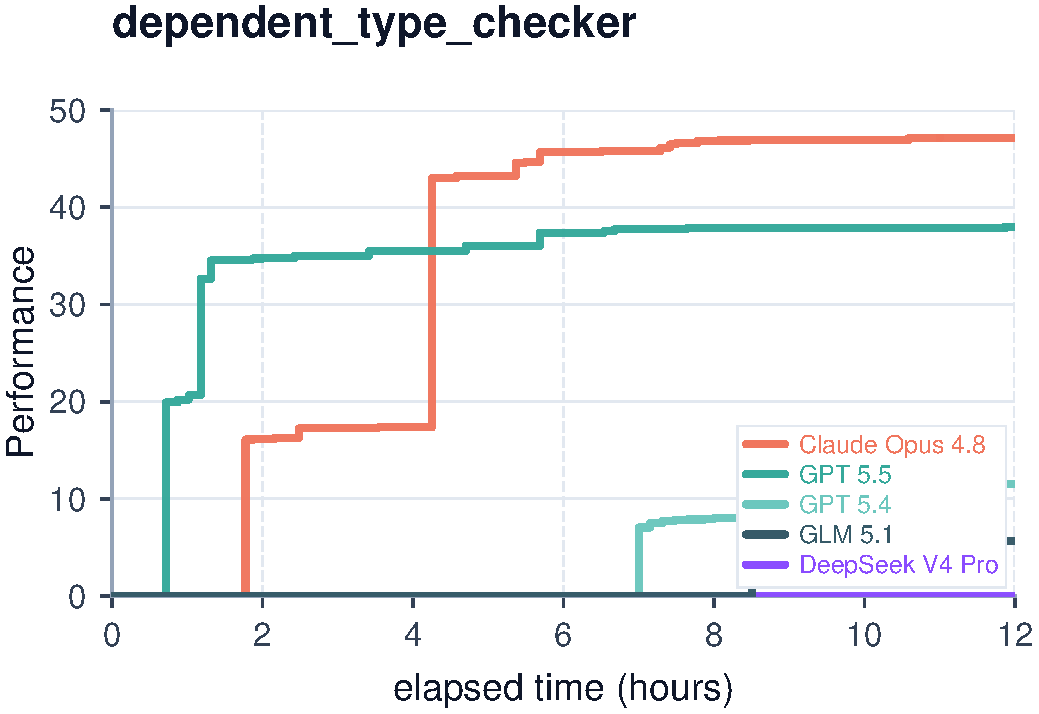
\includegraphics[width=\linewidth]{figures/curves/dependent_type_checker_time_performance.pdf}
\end{subfigure}
\vspace{0.5em}
\begin{subfigure}[b]{0.48\linewidth}
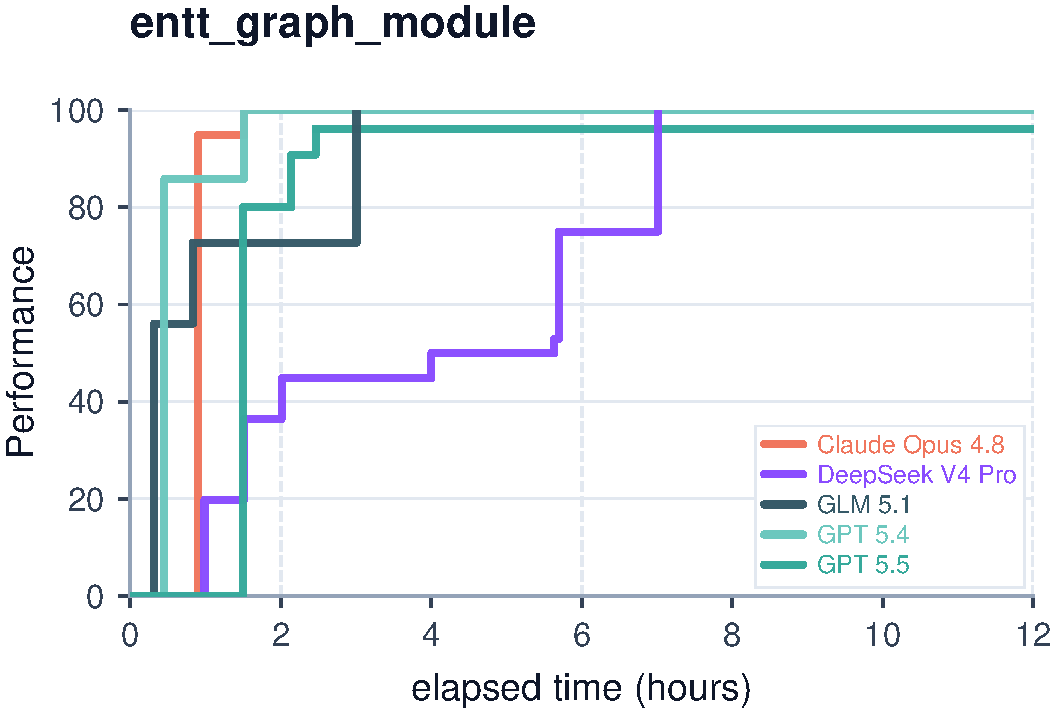
\includegraphics[width=\linewidth]{figures/curves/entt_graph_time_performance.pdf}
\end{subfigure}
\hfill
\begin{subfigure}[b]{0.48\linewidth}
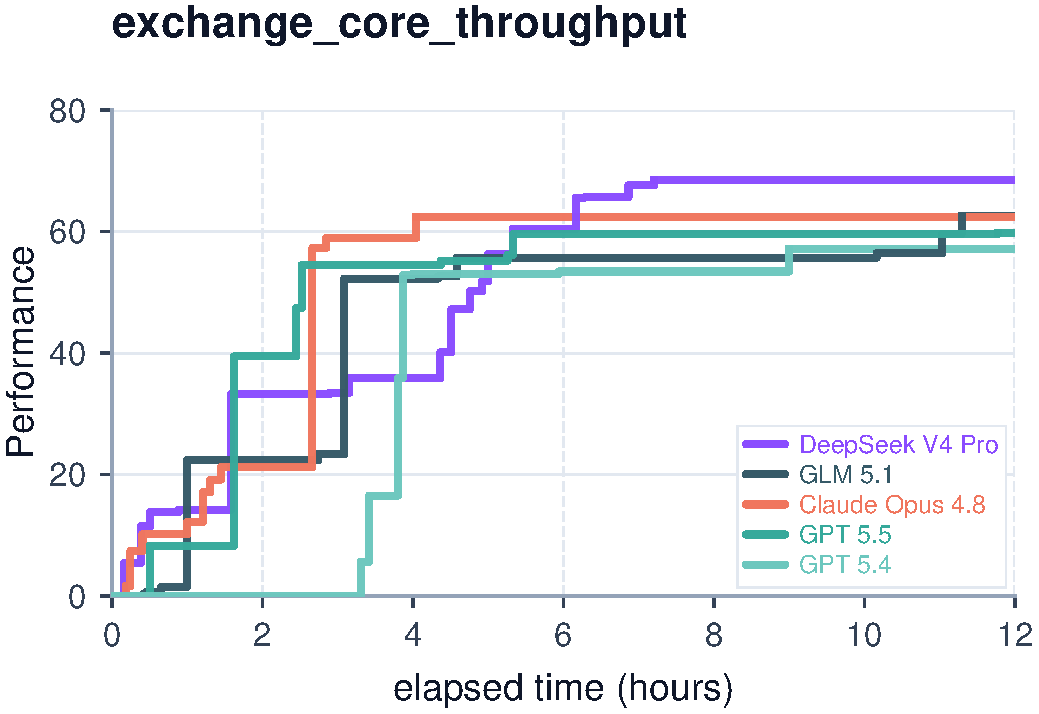
\includegraphics[width=\linewidth]{figures/curves/exchange_core_time_performance.pdf}
\end{subfigure}
\caption{Per-task learning curves: Systems \& Software Engineering (7/21).}
\label{fig:curves-all-7}
\end{figure}

\begin{figure}[p]
\centering
\begin{subfigure}[b]{0.48\linewidth}
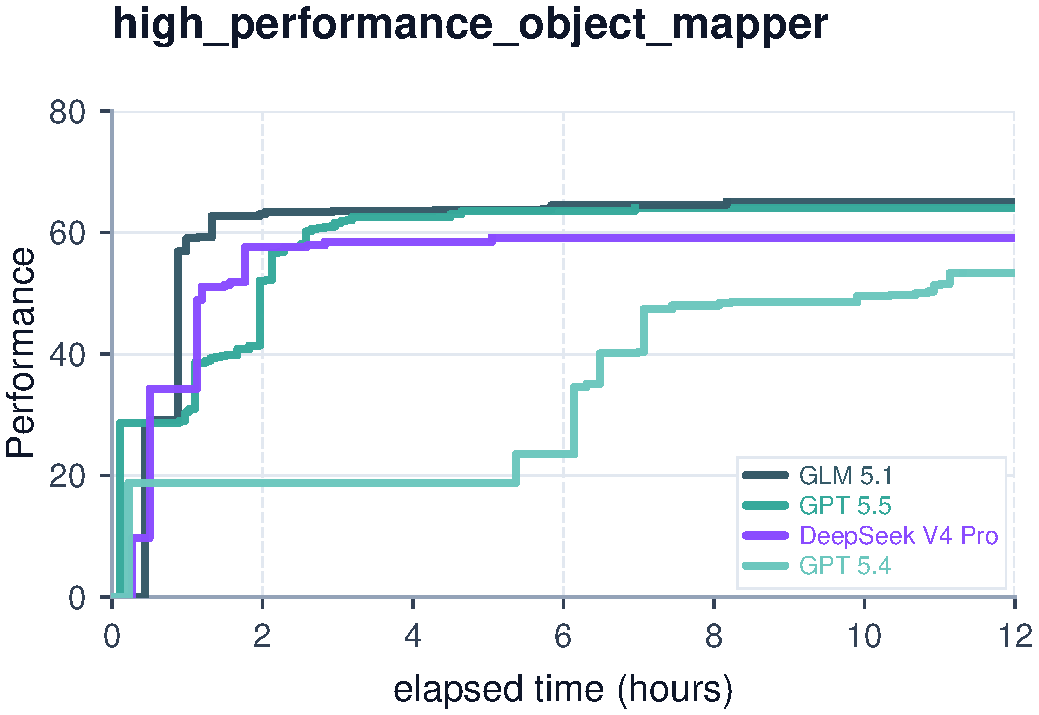
\includegraphics[width=\linewidth]{figures/curves/high_performance_object_mapper_time_performance.pdf}
\end{subfigure}
\hfill
\begin{subfigure}[b]{0.48\linewidth}
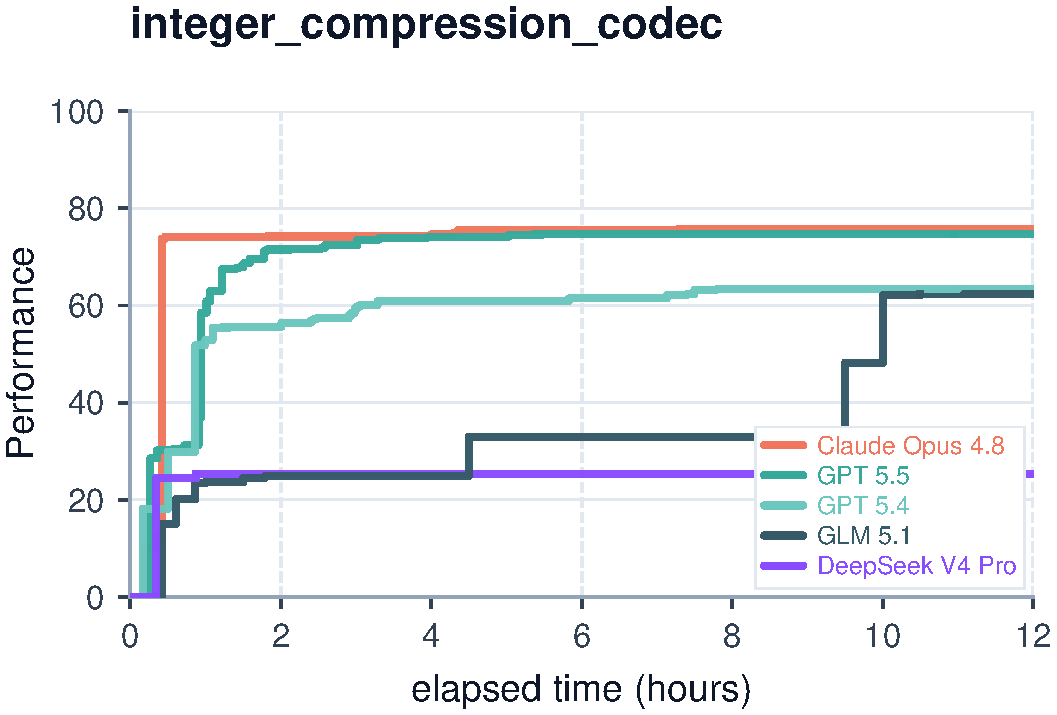
\includegraphics[width=\linewidth]{figures/curves/integer_compression_codec_time_performance.pdf}
\end{subfigure}
\vspace{0.5em}
\begin{subfigure}[b]{0.48\linewidth}
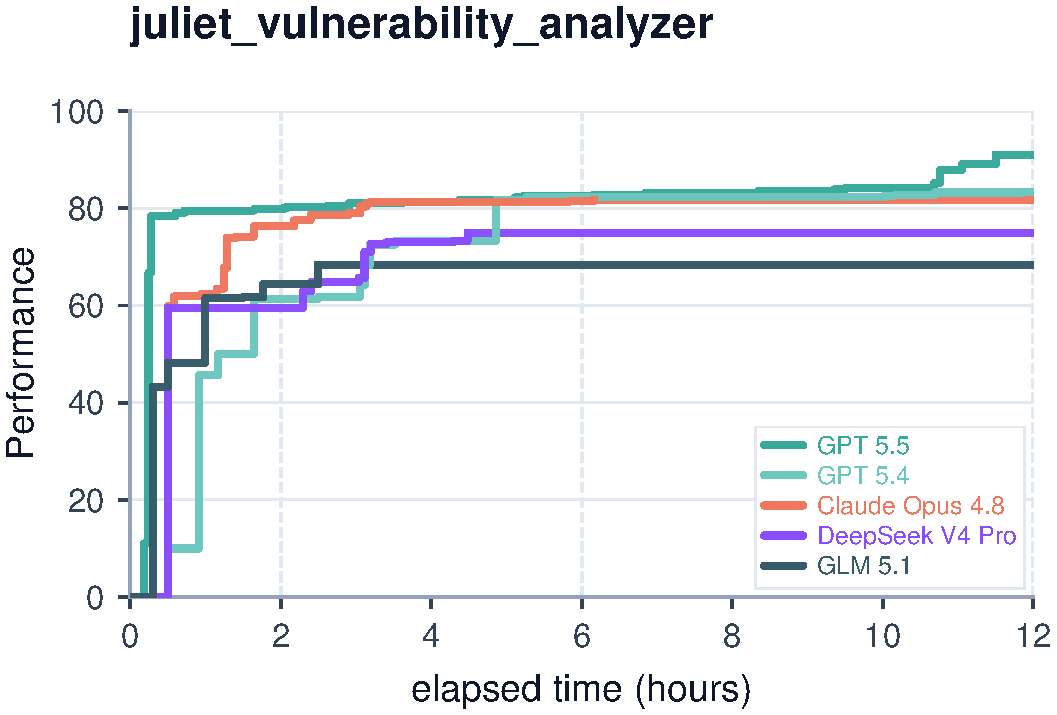
\includegraphics[width=\linewidth]{figures/curves/juliet_static_analyzer_time_performance.pdf}
\end{subfigure}
\hfill
\begin{subfigure}[b]{0.48\linewidth}
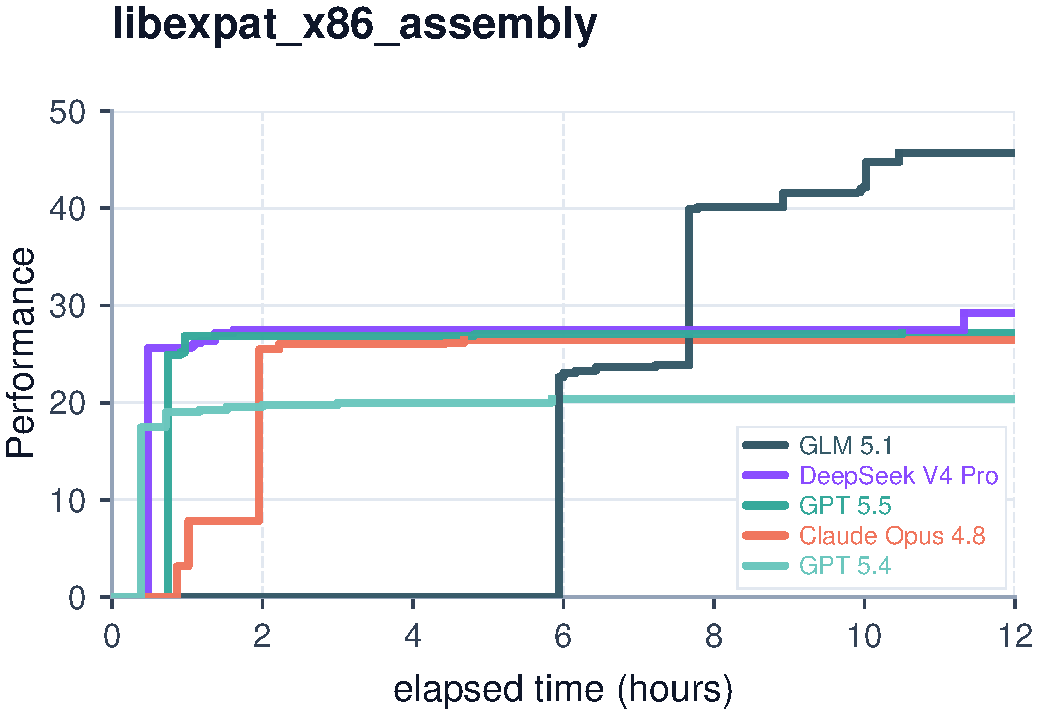
\includegraphics[width=\linewidth]{figures/curves/libexpat_to_x86asm_time_performance.pdf}
\end{subfigure}
\vspace{0.5em}
\begin{subfigure}[b]{0.48\linewidth}
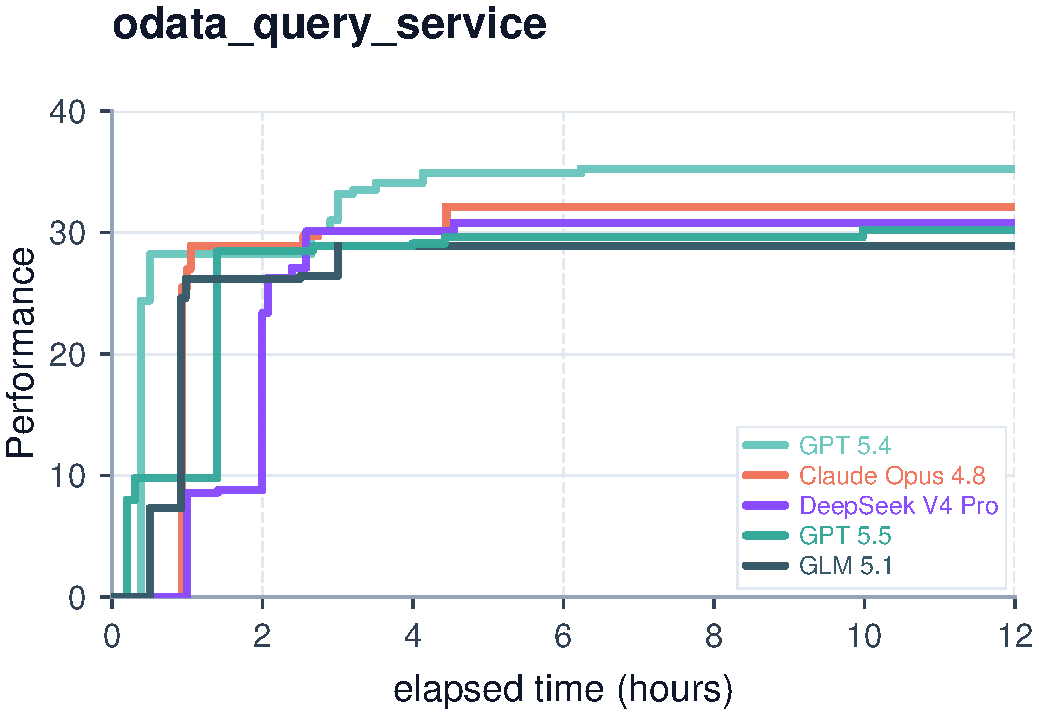
\includegraphics[width=\linewidth]{figures/curves/lightquery_odata_service_time_performance.pdf}
\end{subfigure}
\hfill
\begin{subfigure}[b]{0.48\linewidth}
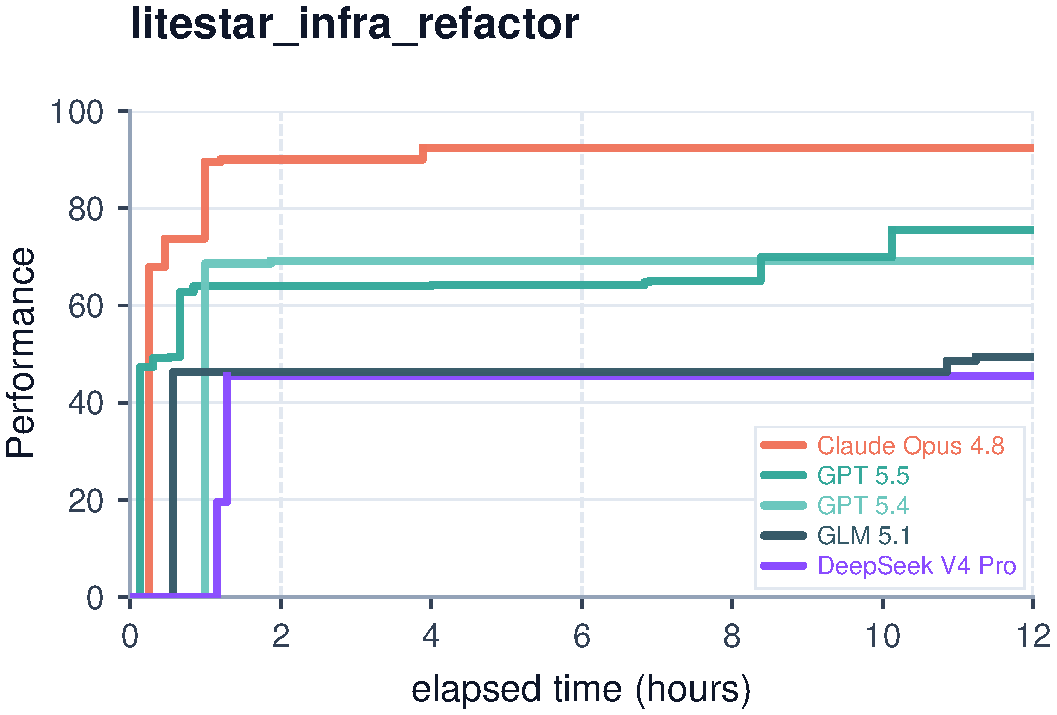
\includegraphics[width=\linewidth]{figures/curves/litestar_infra_time_performance.pdf}
\end{subfigure}
\caption{Per-task learning curves: Systems \& Software Engineering cont. (8/21).}
\label{fig:curves-all-8}
\end{figure}

\begin{figure}[p]
\centering
\begin{subfigure}[b]{0.48\linewidth}
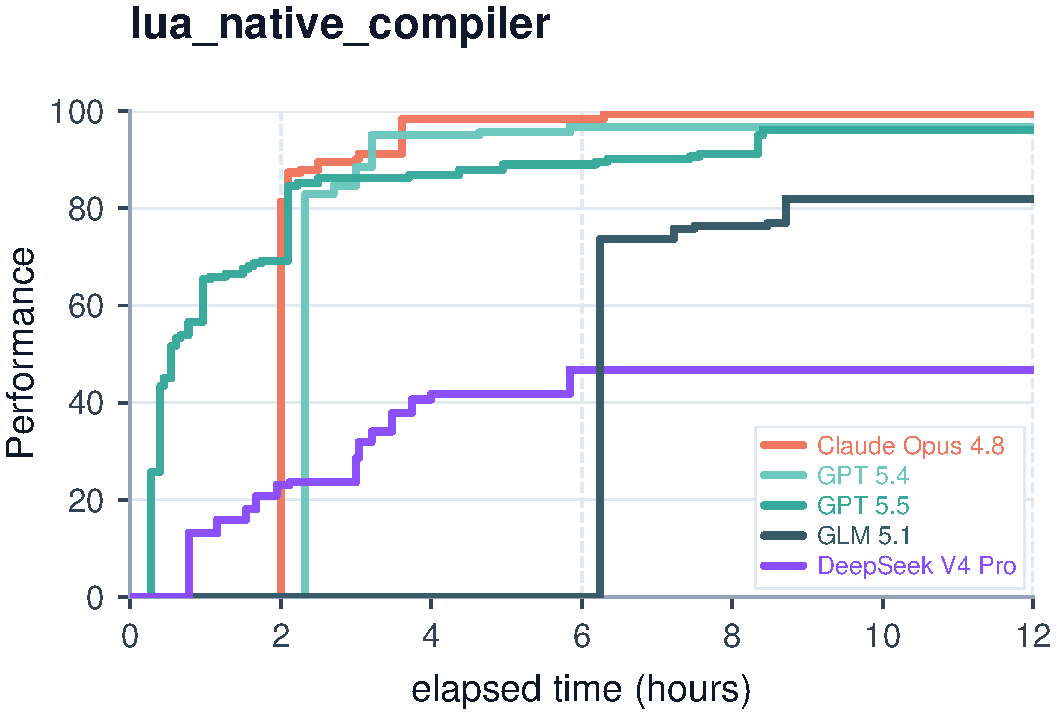
\includegraphics[width=\linewidth]{figures/curves/lua_native_compiler_time_performance.pdf}
\end{subfigure}
\hfill
\begin{subfigure}[b]{0.48\linewidth}
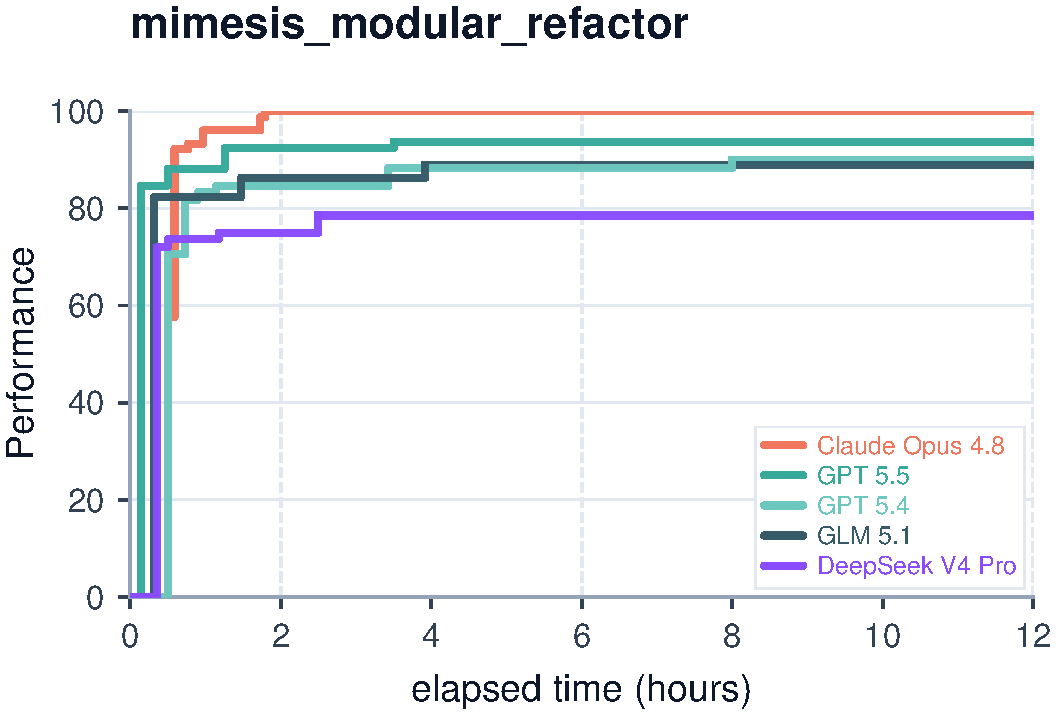
\includegraphics[width=\linewidth]{figures/curves/mimesis_modular_time_performance.pdf}
\end{subfigure}
\vspace{0.5em}
\begin{subfigure}[b]{0.48\linewidth}
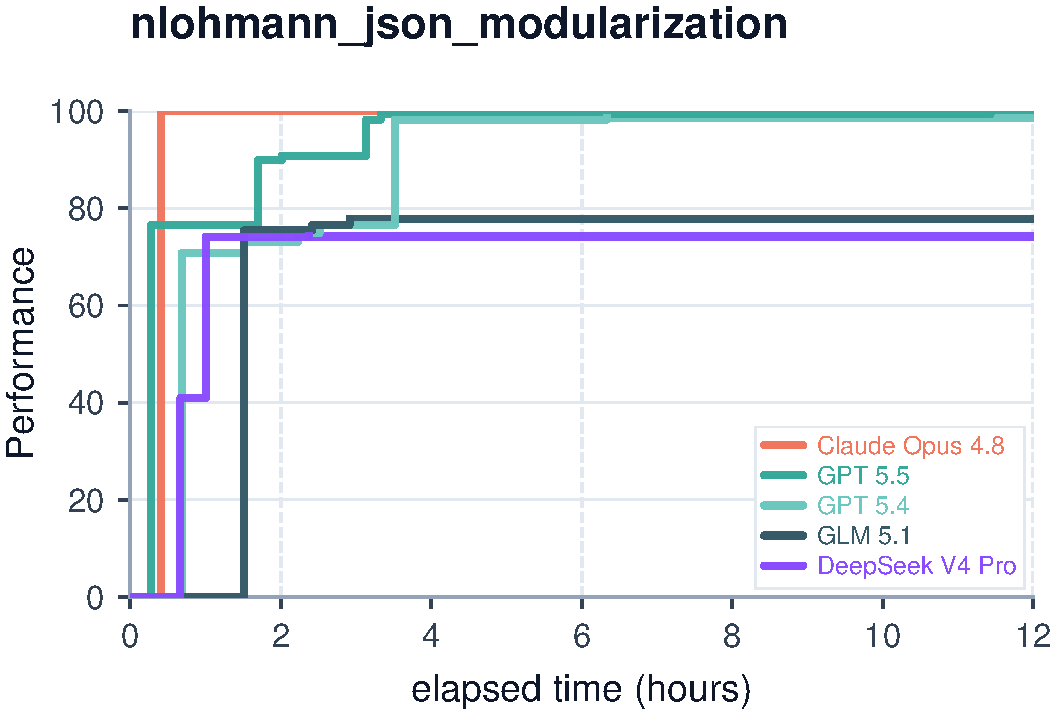
\includegraphics[width=\linewidth]{figures/curves/nlohmann_json_time_performance.pdf}
\end{subfigure}
\hfill
\begin{subfigure}[b]{0.48\linewidth}
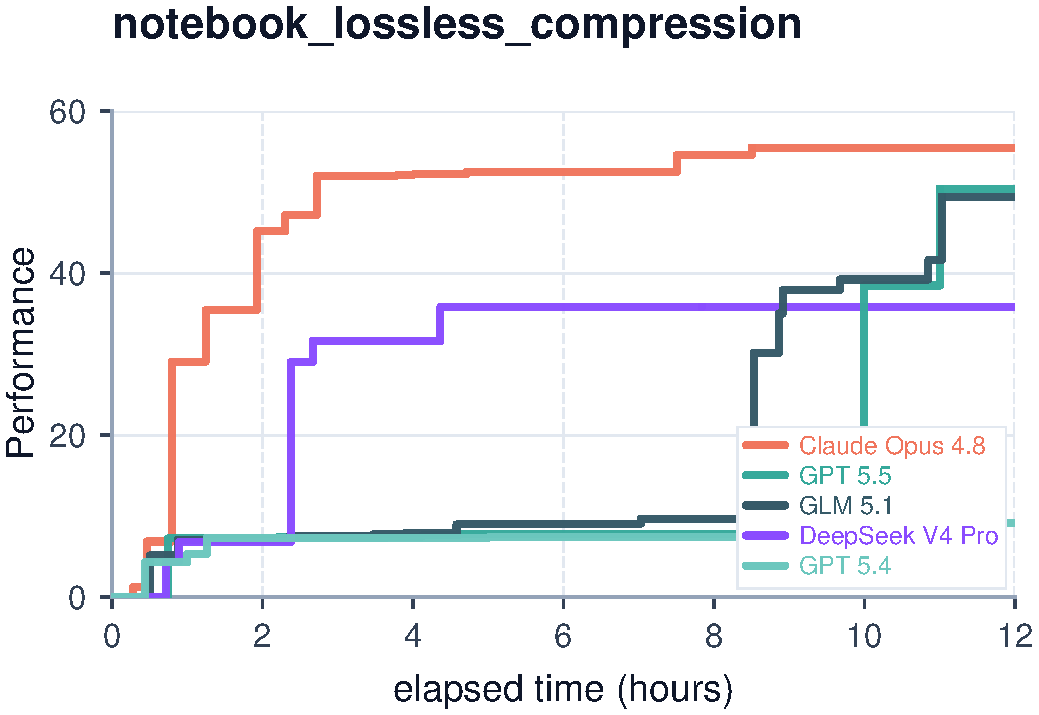
\includegraphics[width=\linewidth]{figures/curves/notebook_compression_time_performance.pdf}
\end{subfigure}
\vspace{0.5em}
\begin{subfigure}[b]{0.48\linewidth}
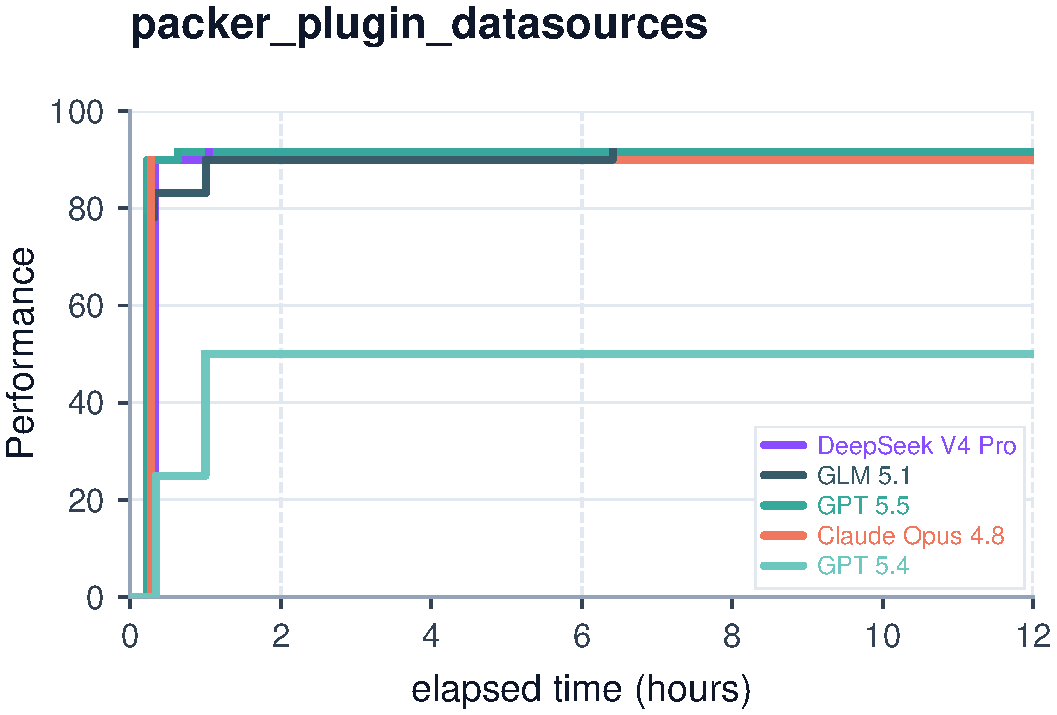
\includegraphics[width=\linewidth]{figures/curves/packer_plugins_time_performance.pdf}
\end{subfigure}
\hfill
\begin{subfigure}[b]{0.48\linewidth}
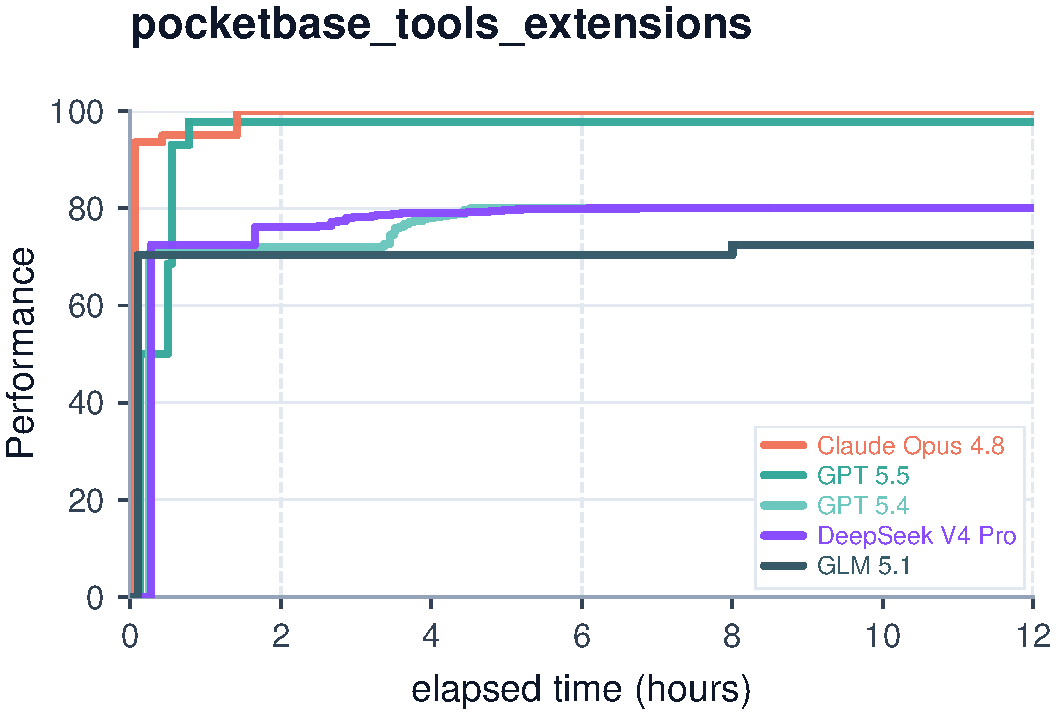
\includegraphics[width=\linewidth]{figures/curves/pocketbase_tools_time_performance.pdf}
\end{subfigure}
\caption{Per-task learning curves: Systems \& Software Engineering cont. (9/21).}
\label{fig:curves-all-9}
\end{figure}

\begin{figure}[p]
\centering
\begin{subfigure}[b]{0.48\linewidth}
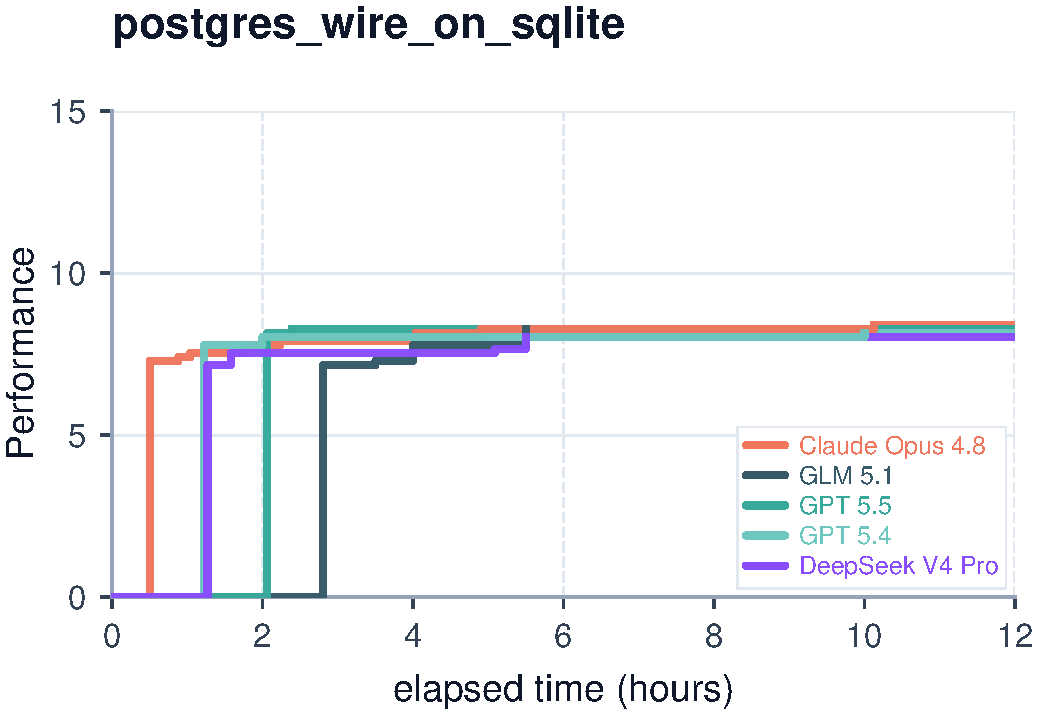
\includegraphics[width=\linewidth]{figures/curves/postgres_sqlite_wire_adapter_time_performance.pdf}
\end{subfigure}
\hfill
\begin{subfigure}[b]{0.48\linewidth}
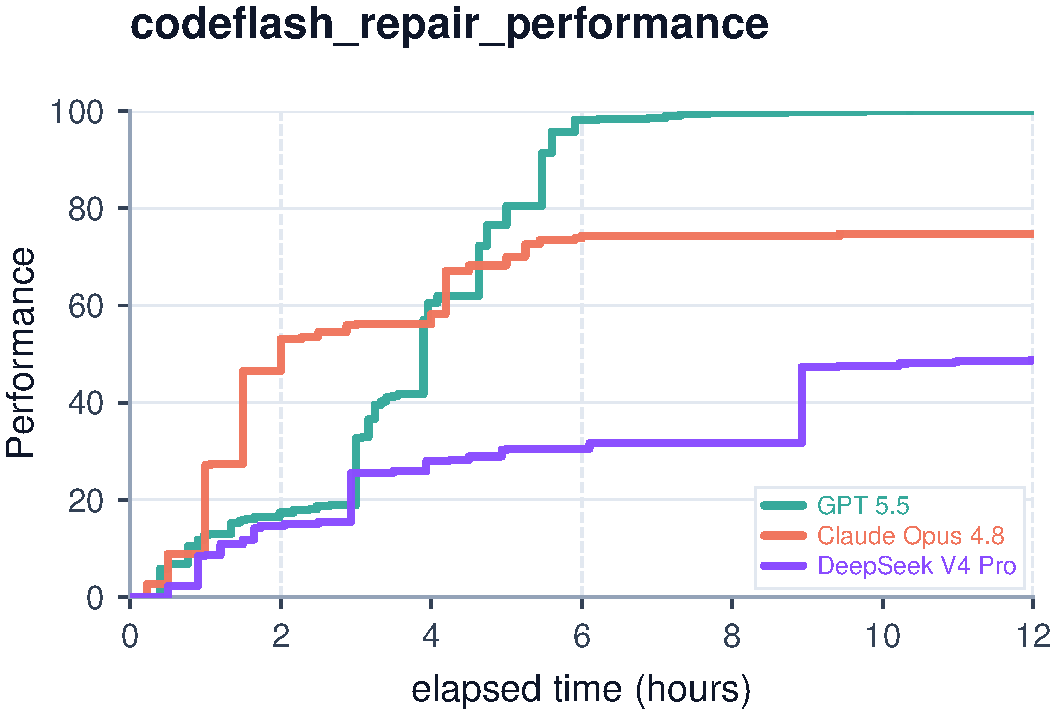
\includegraphics[width=\linewidth]{figures/curves/codeflash_repair_time_performance.pdf}
\end{subfigure}
\vspace{0.5em}
\begin{subfigure}[b]{0.48\linewidth}
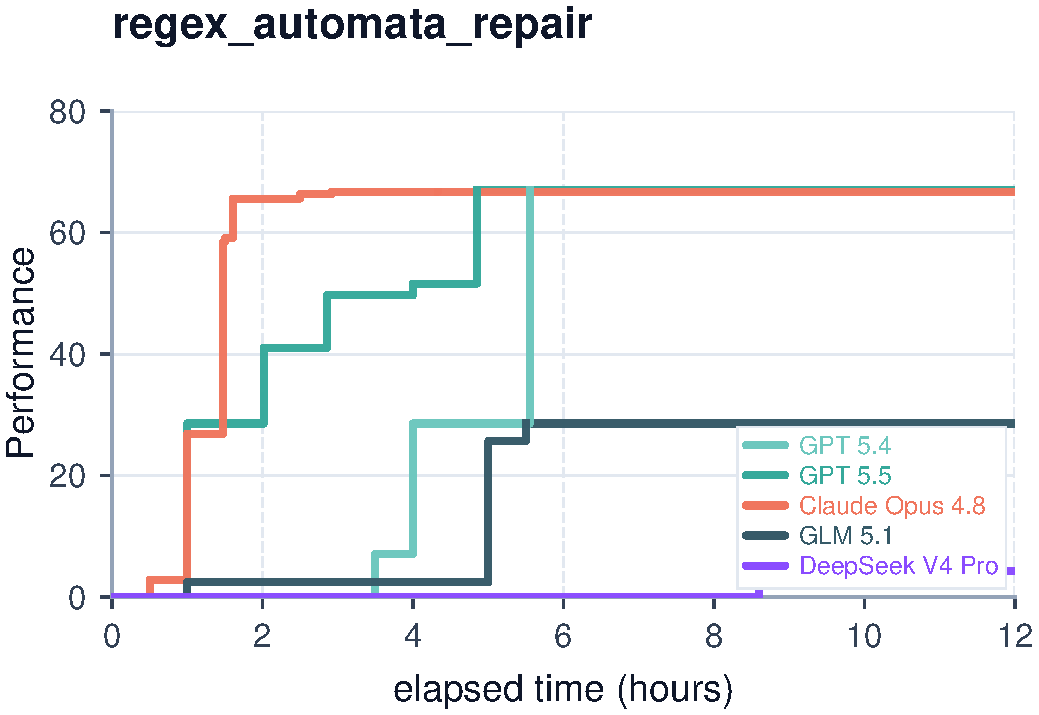
\includegraphics[width=\linewidth]{figures/curves/regex_automata_repair_time_performance.pdf}
\end{subfigure}
\hfill
\begin{subfigure}[b]{0.48\linewidth}
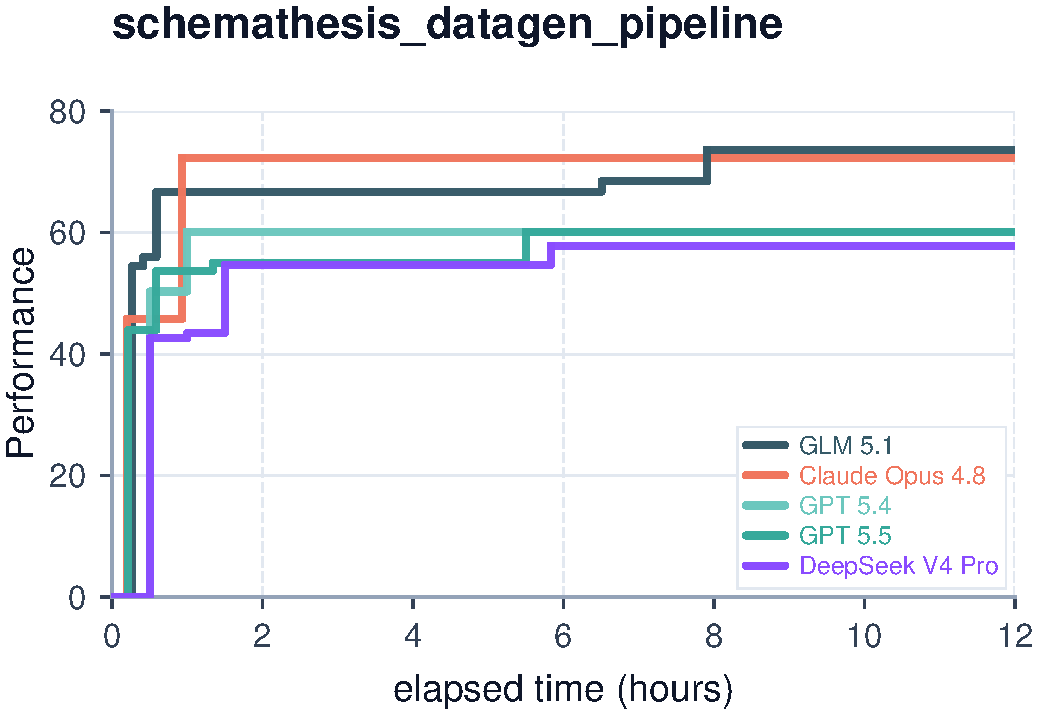
\includegraphics[width=\linewidth]{figures/curves/schemathesis_datagen_time_performance.pdf}
\end{subfigure}
\vspace{0.5em}
\begin{subfigure}[b]{0.48\linewidth}
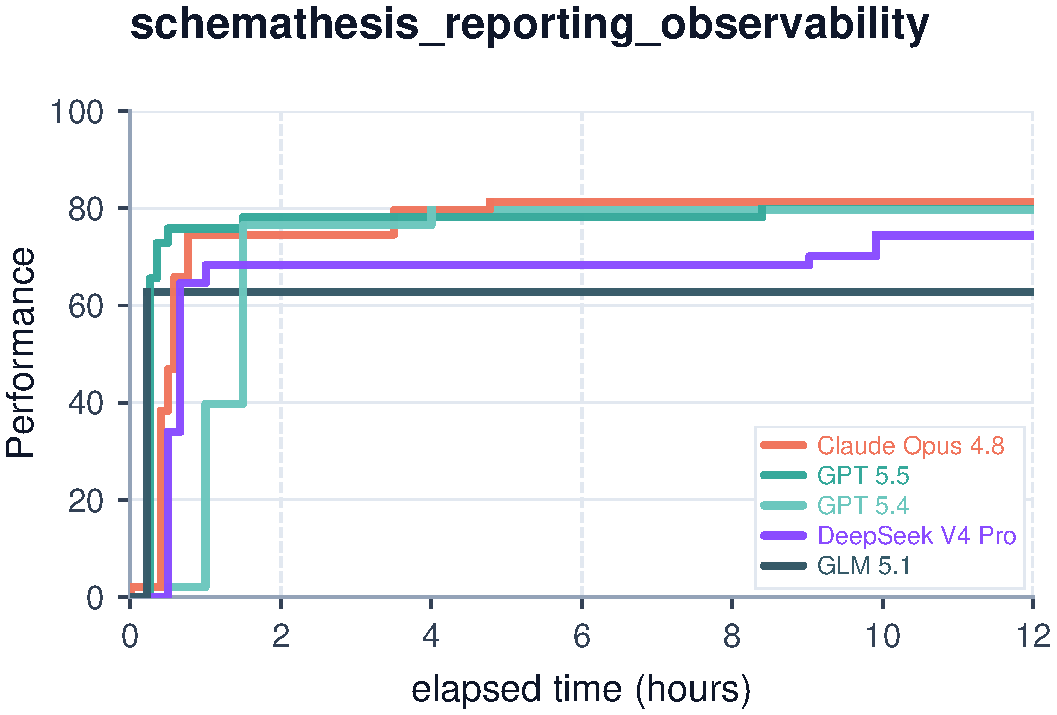
\includegraphics[width=\linewidth]{figures/curves/schemathesis_report_time_performance.pdf}
\end{subfigure}
\hfill
\begin{subfigure}[b]{0.48\linewidth}
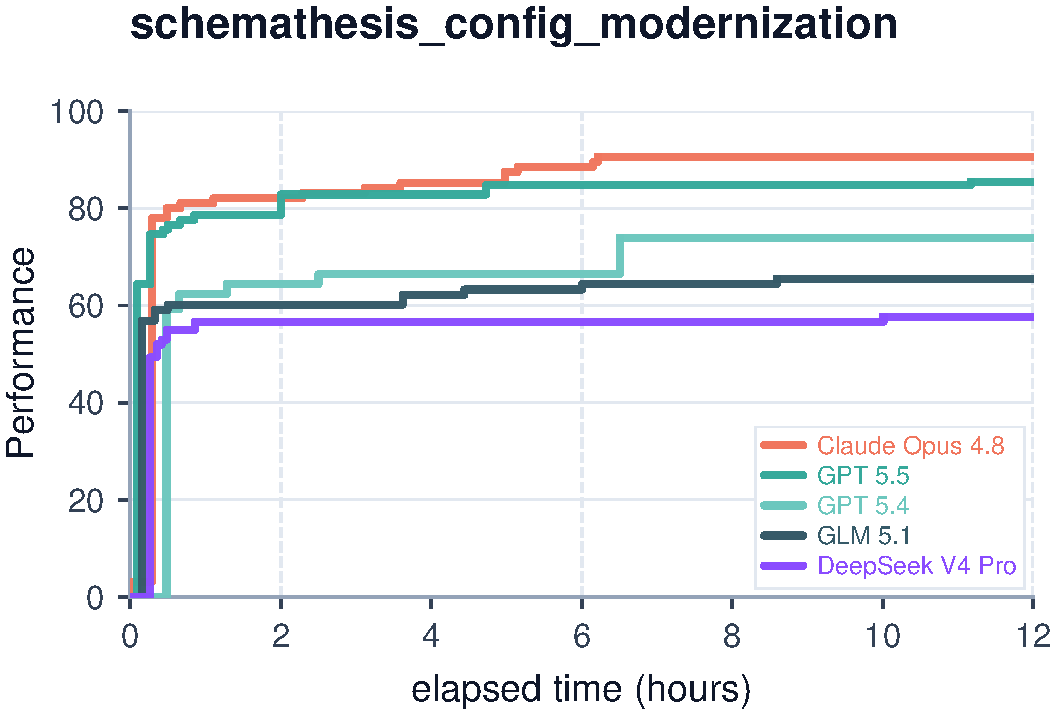
\includegraphics[width=\linewidth]{figures/curves/schemathesis_v4_time_performance.pdf}
\end{subfigure}
\caption{Per-task learning curves: Systems \& Software Engineering cont. (10/21).}
\label{fig:curves-all-10}
\end{figure}

\begin{figure}[p]
\centering
\begin{subfigure}[b]{0.48\linewidth}
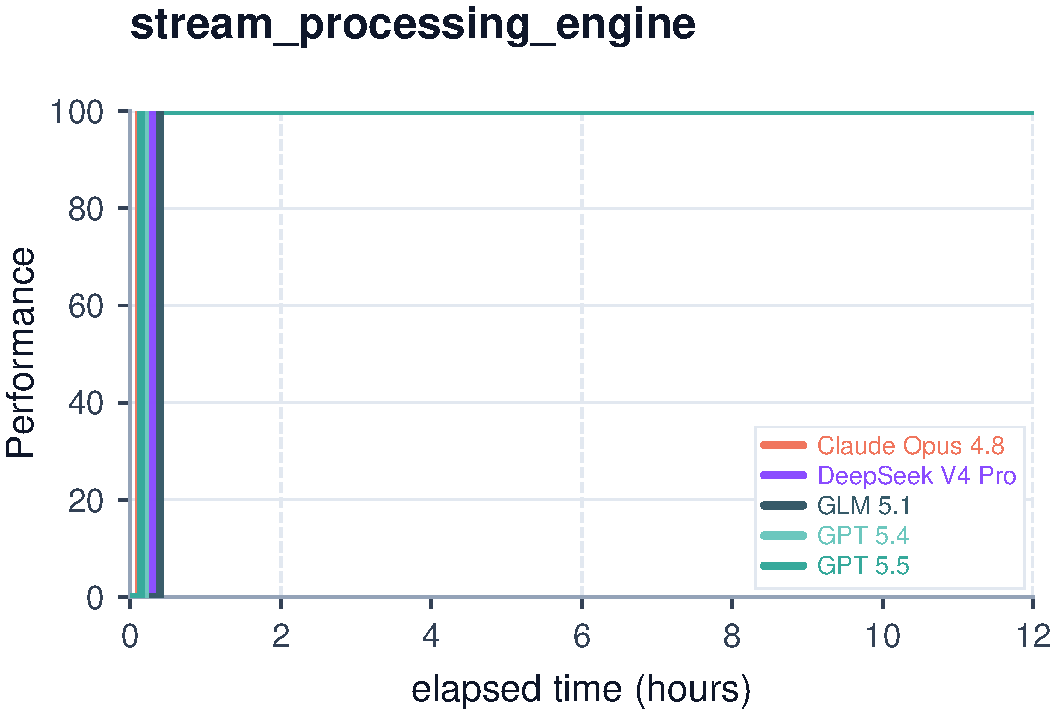
\includegraphics[width=\linewidth]{figures/curves/stream_processing_pipeline_time_performance.pdf}
\end{subfigure}
\hfill
\begin{subfigure}[b]{0.48\linewidth}
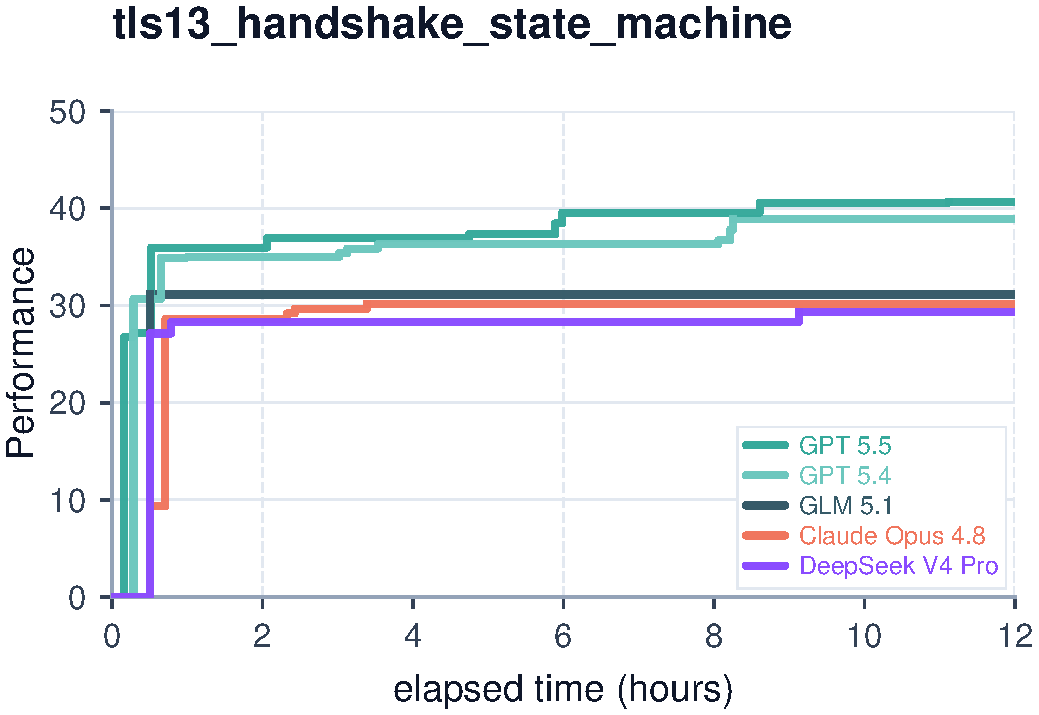
\includegraphics[width=\linewidth]{figures/curves/tls13_mini_handshake_state_machine_time_performance.pdf}
\end{subfigure}
\vspace{0.5em}
\begin{subfigure}[b]{0.48\linewidth}
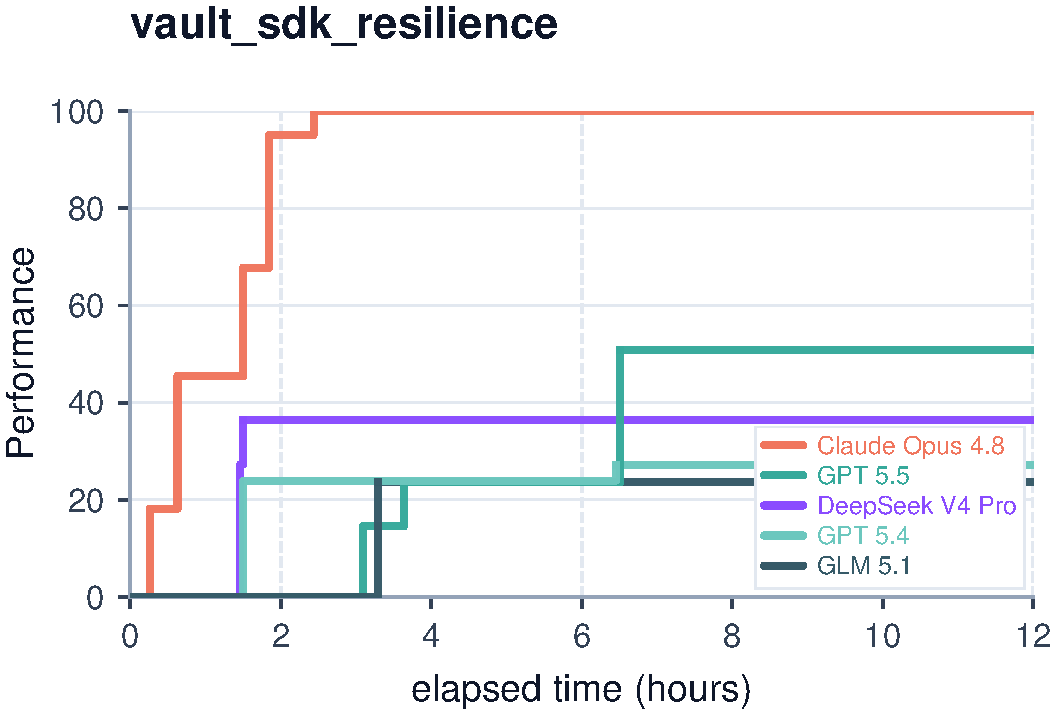
\includegraphics[width=\linewidth]{figures/curves/vault_sdk_time_performance.pdf}
\end{subfigure}
\hfill
\begin{subfigure}[b]{0.48\linewidth}
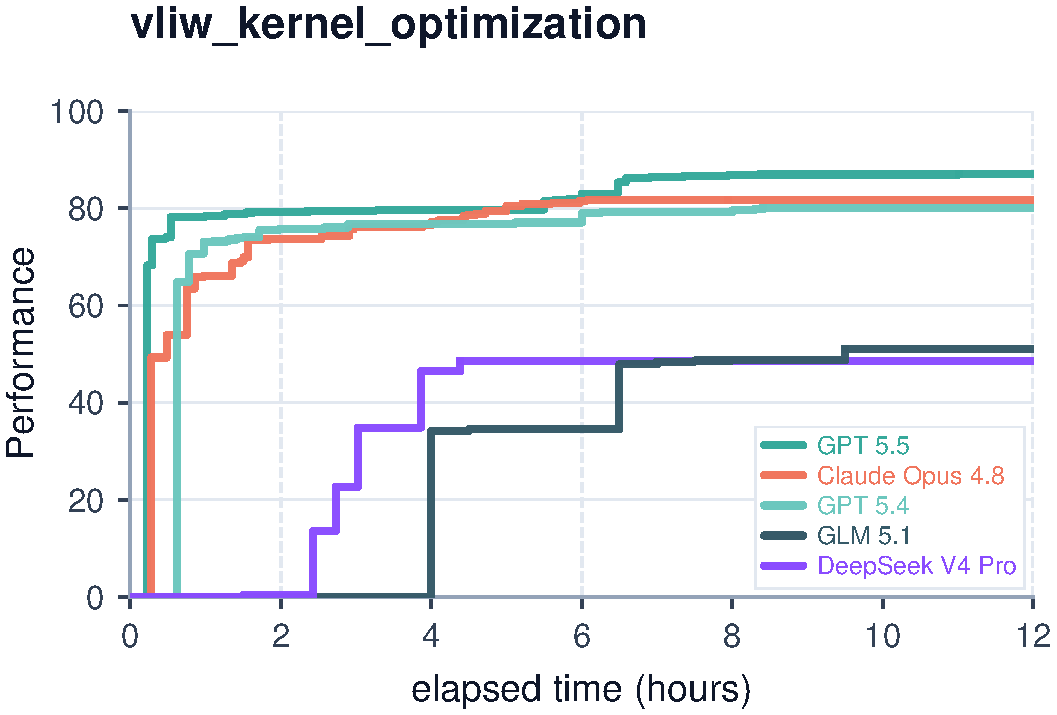
\includegraphics[width=\linewidth]{figures/curves/vliw_kernel_time_performance.pdf}
\end{subfigure}
\vspace{0.5em}
\begin{subfigure}[b]{0.48\linewidth}
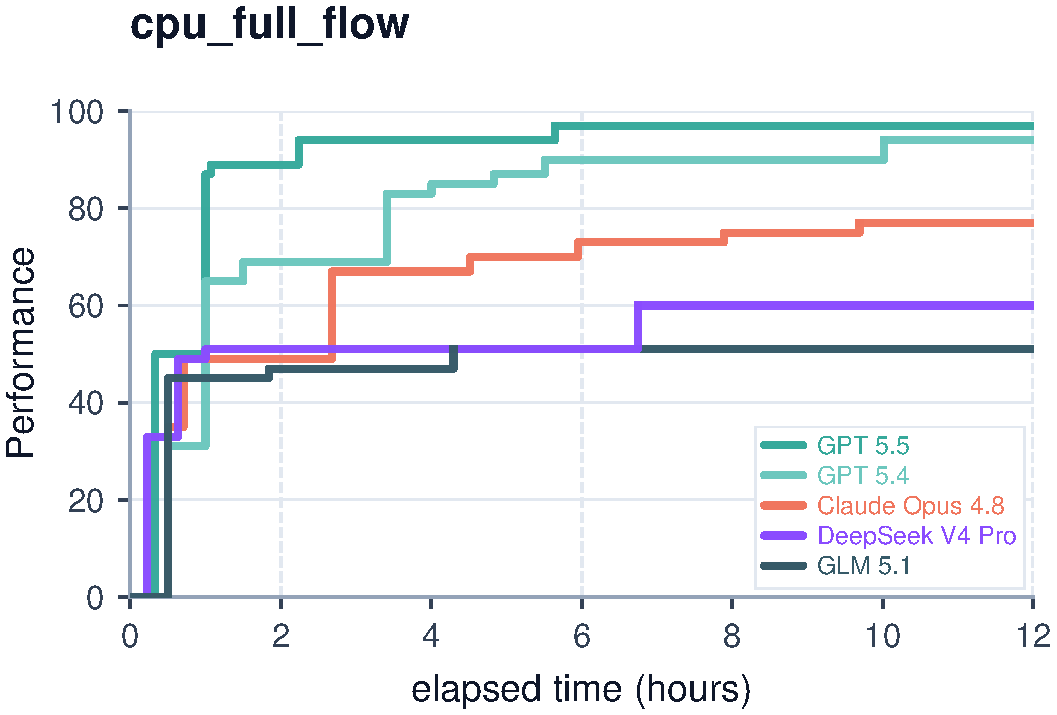
\includegraphics[width=\linewidth]{figures/curves/ysyx_full_time_performance.pdf}
\end{subfigure}
\hfill
\begin{subfigure}[b]{0.48\linewidth}
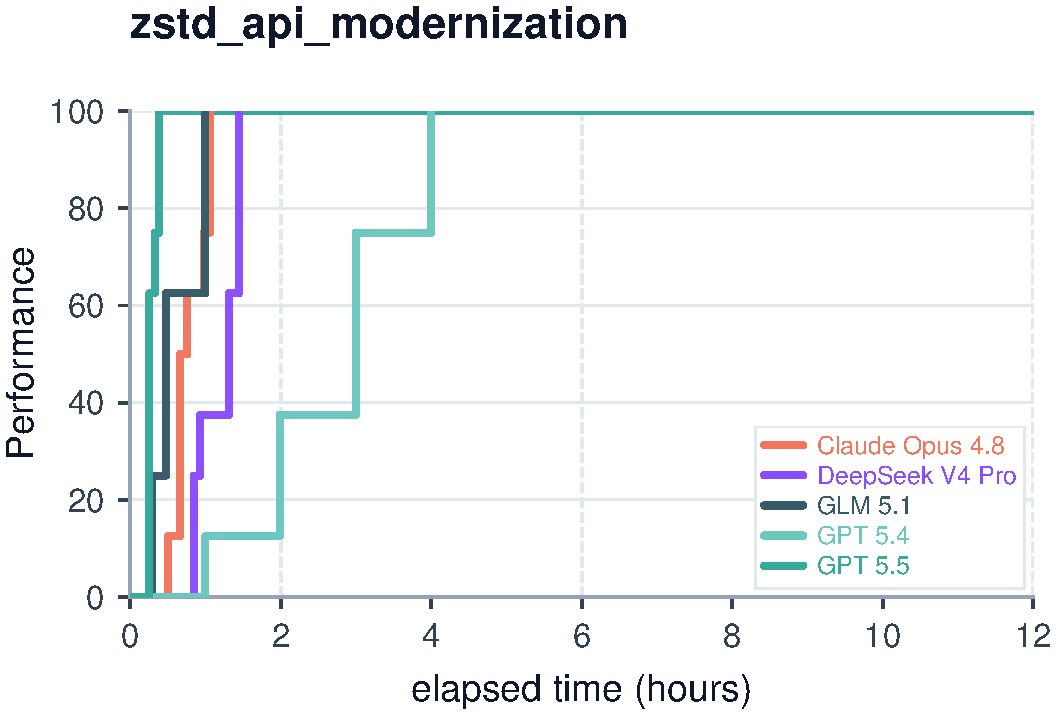
\includegraphics[width=\linewidth]{figures/curves/zstd_api_time_performance.pdf}
\end{subfigure}
\caption{Per-task learning curves: Systems \& Software Engineering cont. (11/21).}
\label{fig:curves-all-11}
\end{figure}

\begin{figure}[p]
\centering
\begin{subfigure}[b]{0.48\linewidth}
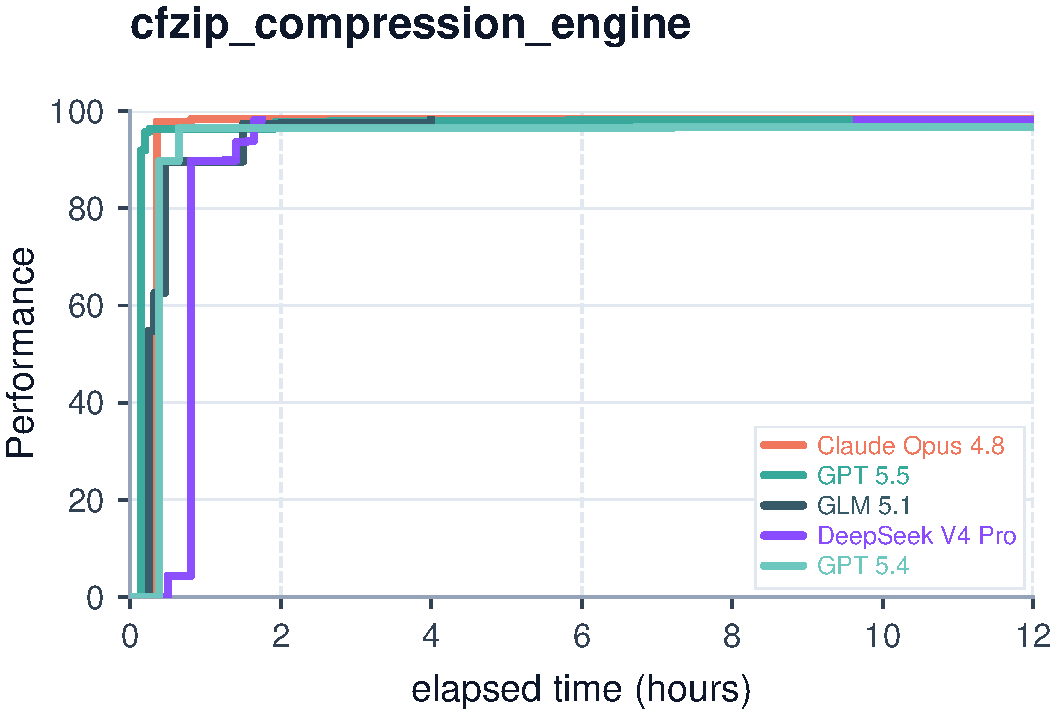
\includegraphics[width=\linewidth]{figures/curves/zstd_compression_engine_time_performance.pdf}
\end{subfigure}
\hfill
\begin{subfigure}[b]{0.48\linewidth}
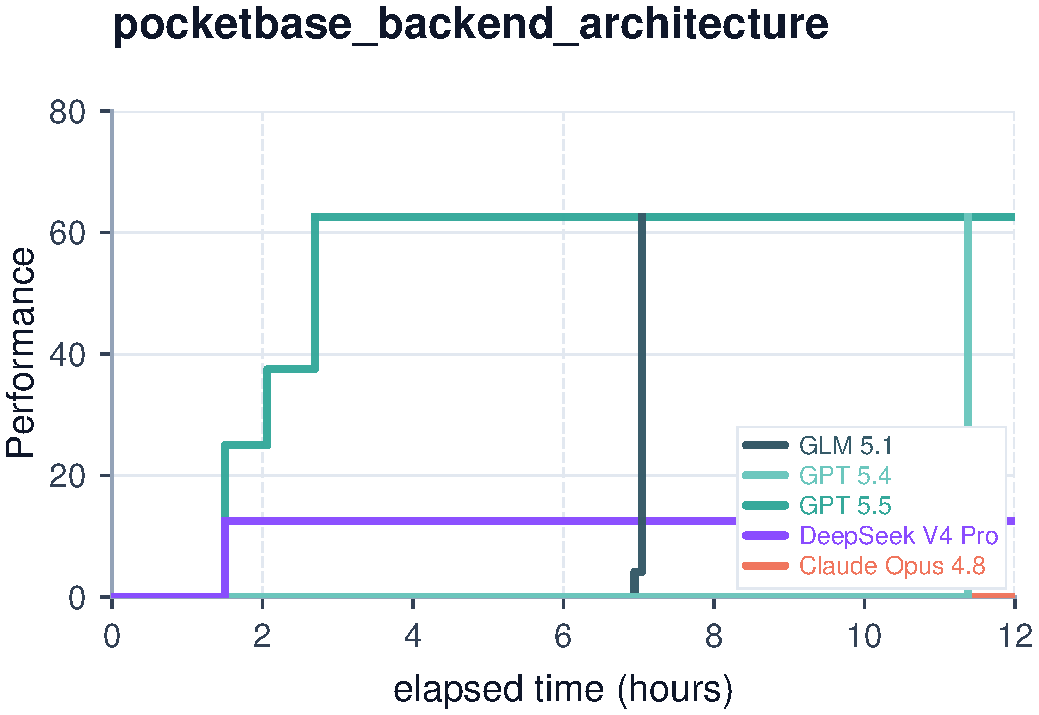
\includegraphics[width=\linewidth]{figures/curves/pocketbase_arch_time_performance.pdf}
\end{subfigure}
\vspace{0.5em}
\begin{subfigure}[b]{0.48\linewidth}
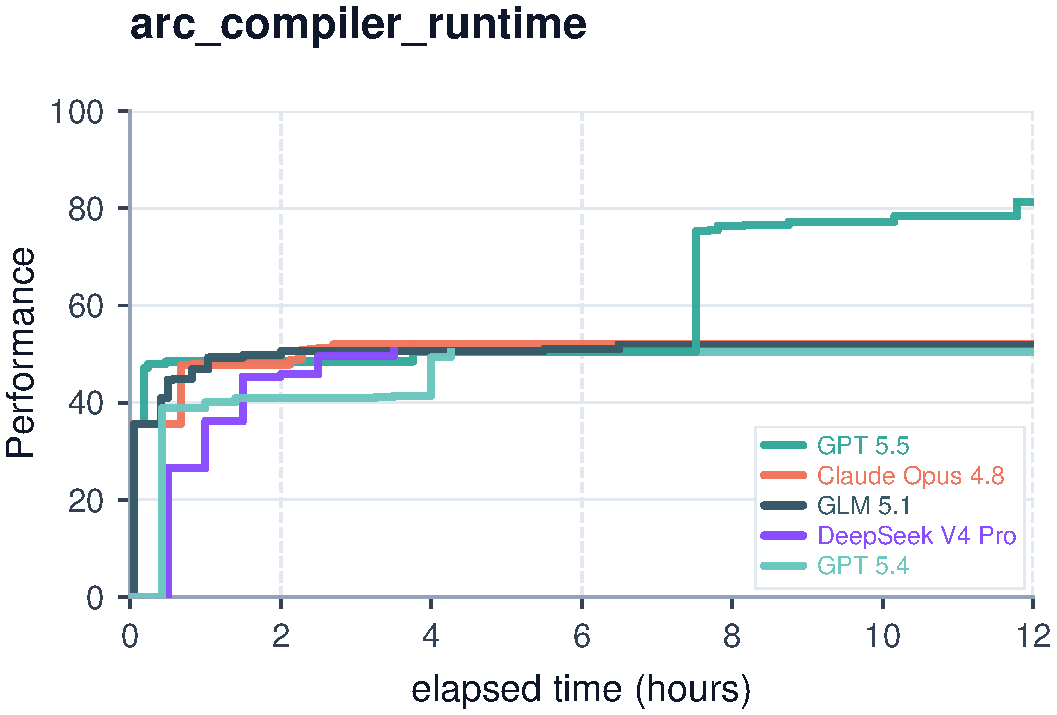
\includegraphics[width=\linewidth]{figures/curves/arc_compiler_runtime_implementation_time_performance.pdf}
\end{subfigure}
\caption{Per-task learning curves: Systems \& Software Engineering cont. (12/21).}
\label{fig:curves-all-12}
\end{figure}

\begin{figure}[p]
\centering
\begin{subfigure}[b]{0.48\linewidth}
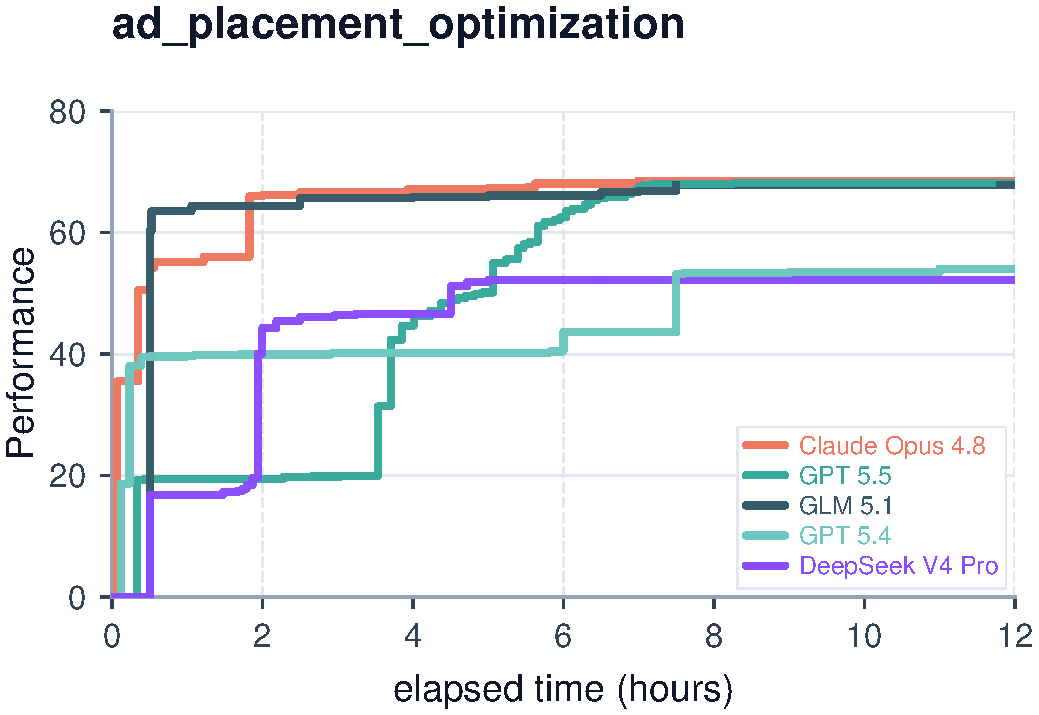
\includegraphics[width=\linewidth]{figures/curves/ad_placement_time_performance.pdf}
\end{subfigure}
\hfill
\begin{subfigure}[b]{0.48\linewidth}
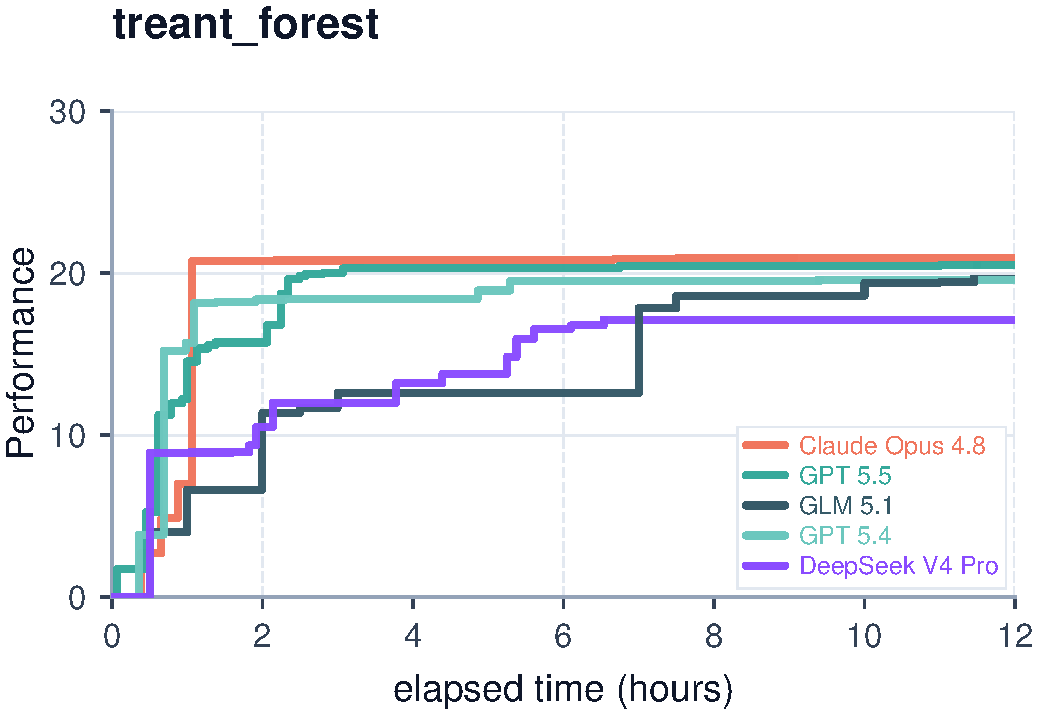
\includegraphics[width=\linewidth]{figures/curves/ahc054_time_performance.pdf}
\end{subfigure}
\vspace{0.5em}
\begin{subfigure}[b]{0.48\linewidth}
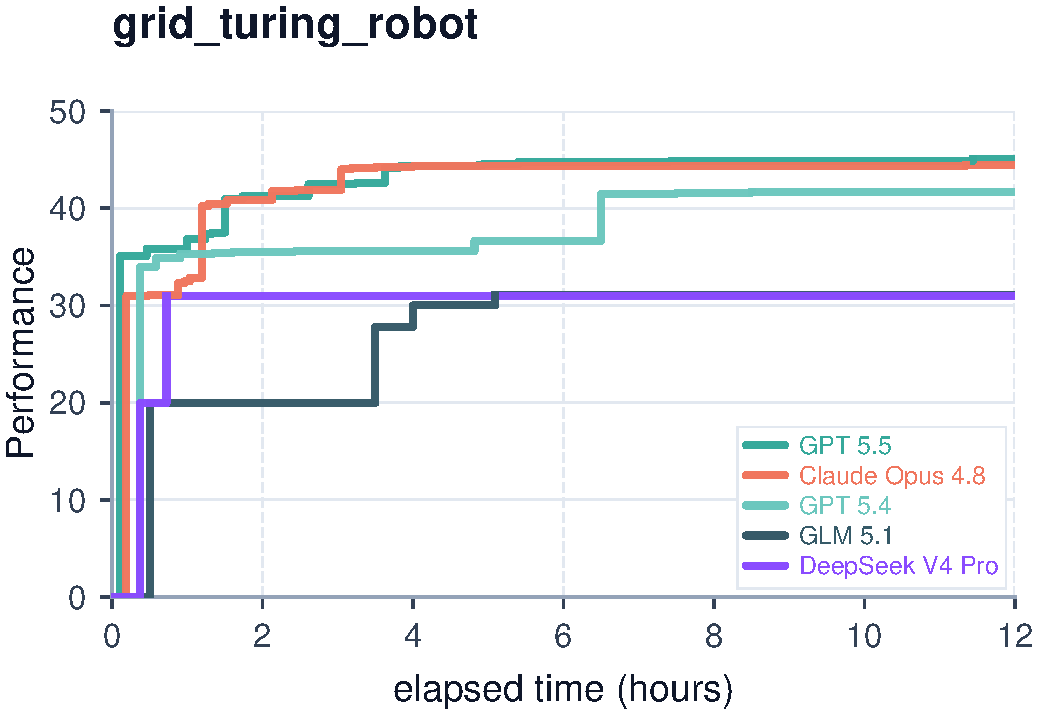
\includegraphics[width=\linewidth]{figures/curves/ahc056_time_performance.pdf}
\end{subfigure}
\hfill
\begin{subfigure}[b]{0.48\linewidth}
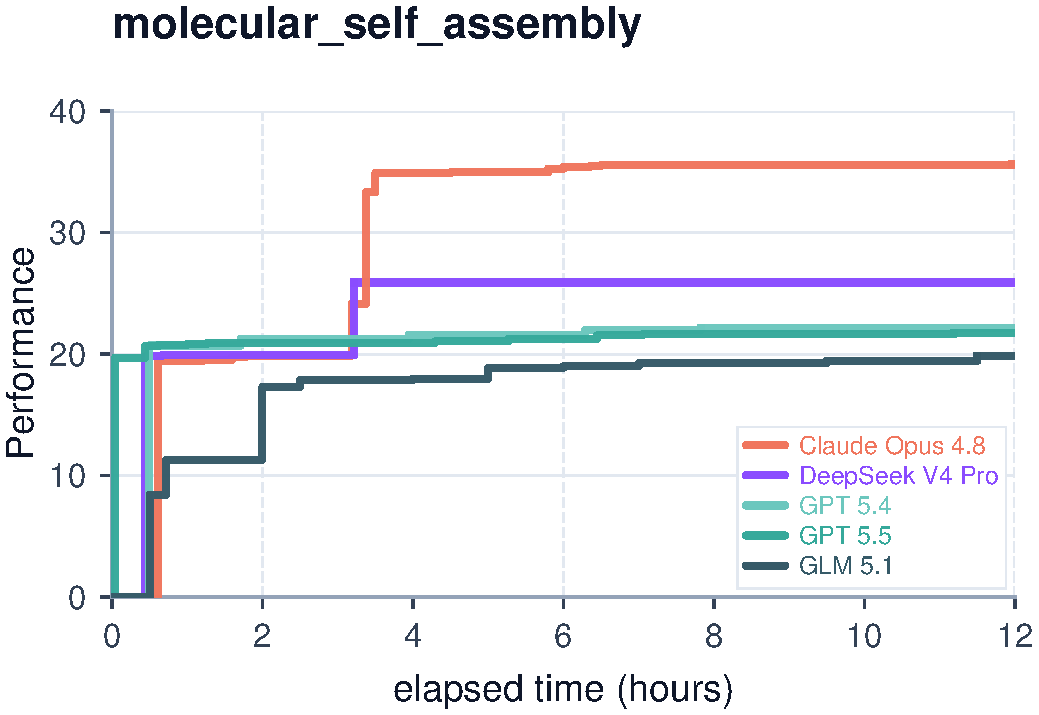
\includegraphics[width=\linewidth]{figures/curves/ahc057_time_performance.pdf}
\end{subfigure}
\vspace{0.5em}
\begin{subfigure}[b]{0.48\linewidth}
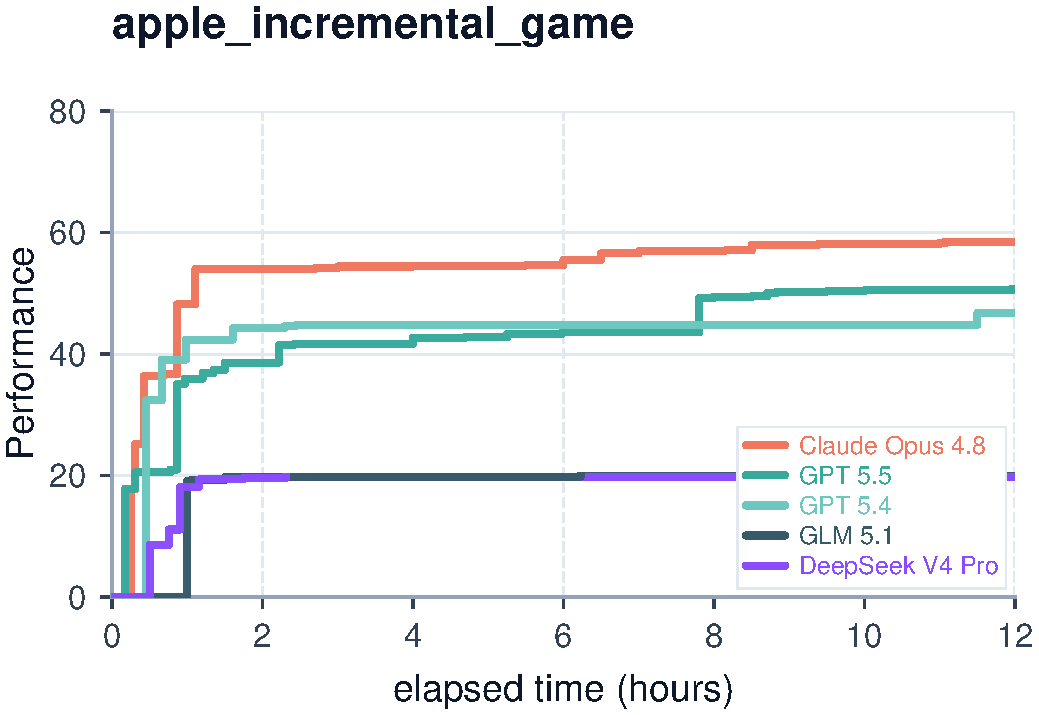
\includegraphics[width=\linewidth]{figures/curves/ahc058_time_performance.pdf}
\end{subfigure}
\hfill
\begin{subfigure}[b]{0.48\linewidth}
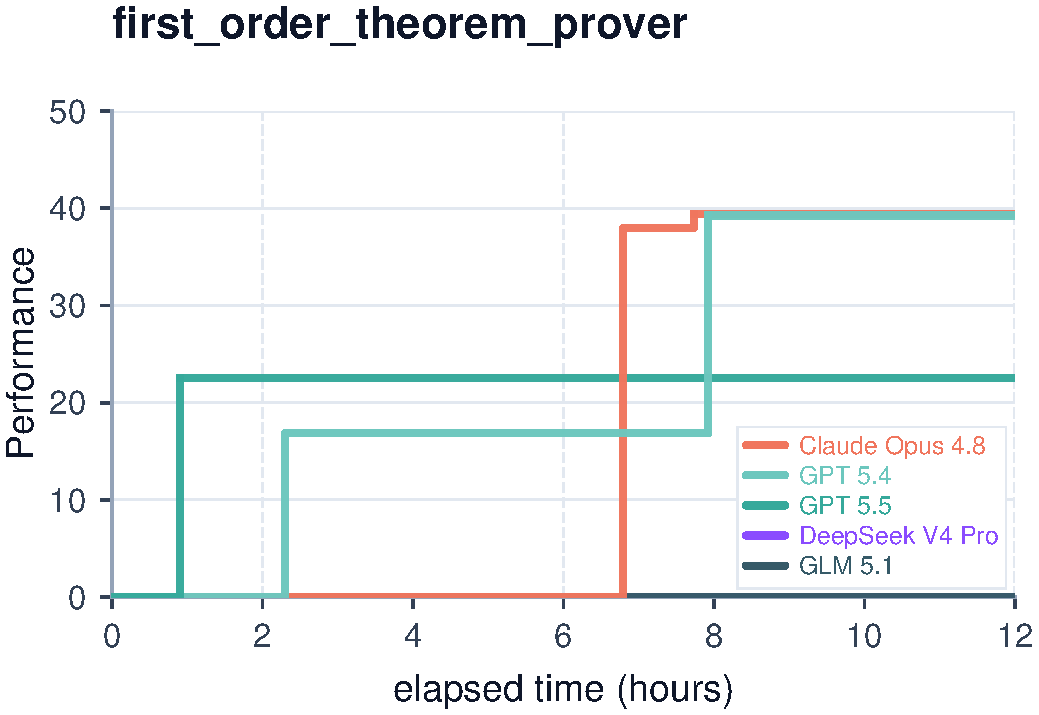
\includegraphics[width=\linewidth]{figures/curves/atp_first_order_prover_time_performance.pdf}
\end{subfigure}
\caption{Per-task learning curves: Combinatorial Optimization \& Planning (13/21).}
\label{fig:curves-all-13}
\end{figure}

\begin{figure}[p]
\centering
\begin{subfigure}[b]{0.48\linewidth}
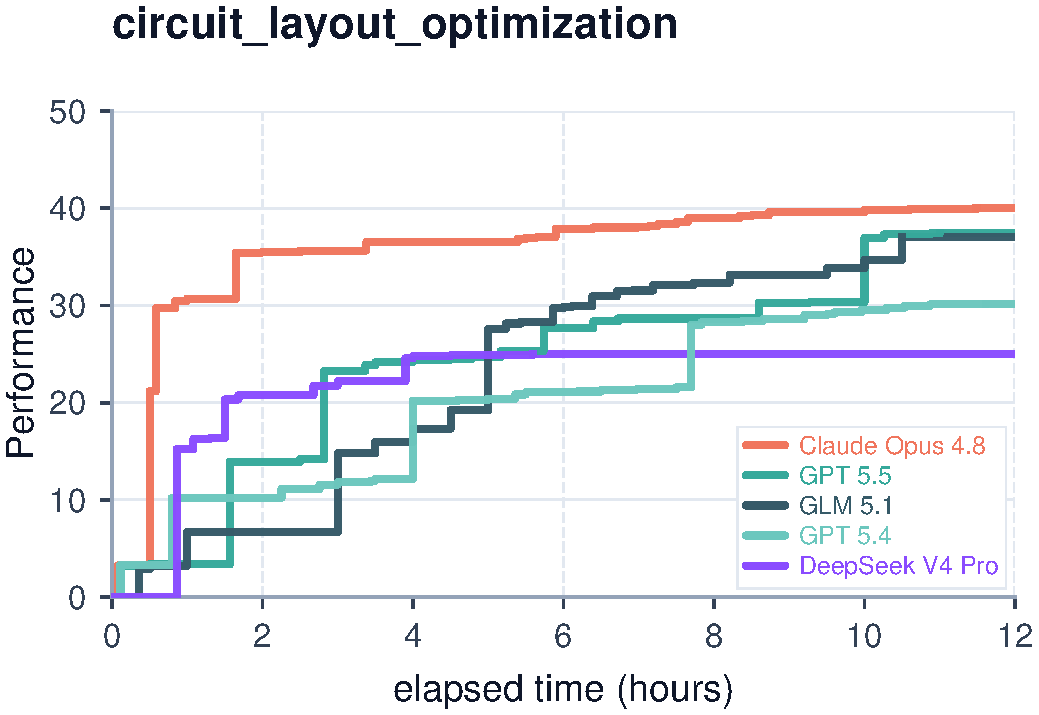
\includegraphics[width=\linewidth]{figures/curves/circuit_layout_optimization_time_performance.pdf}
\end{subfigure}
\hfill
\begin{subfigure}[b]{0.48\linewidth}
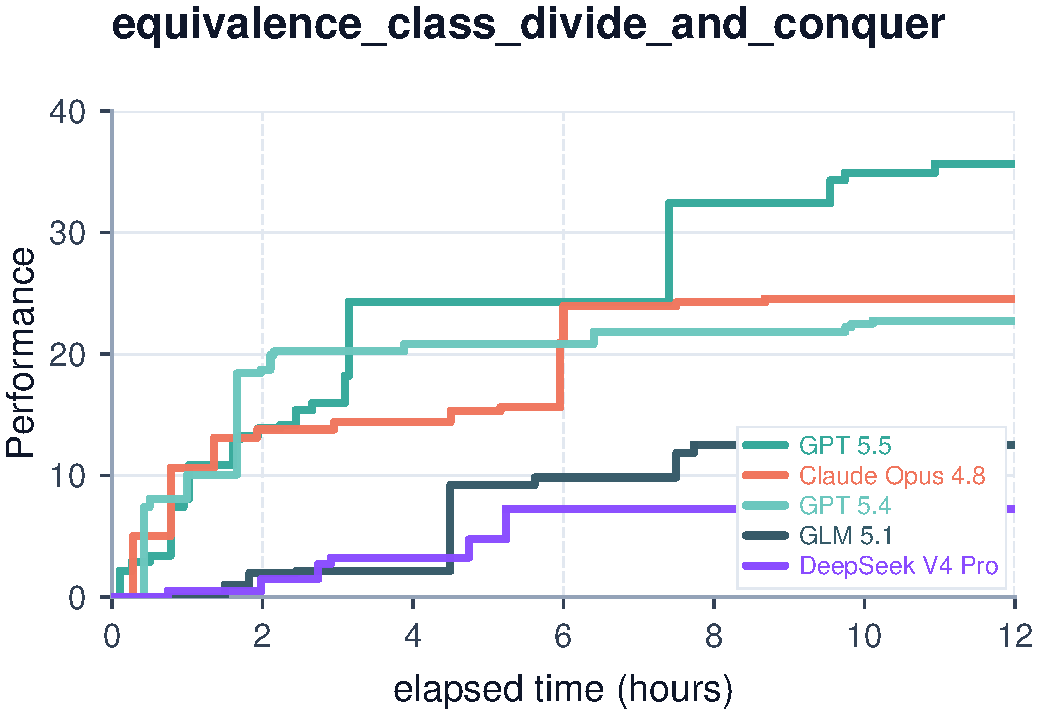
\includegraphics[width=\linewidth]{figures/curves/equivalence_class_divide_and_conquer_time_performance.pdf}
\end{subfigure}
\vspace{0.5em}
\begin{subfigure}[b]{0.48\linewidth}
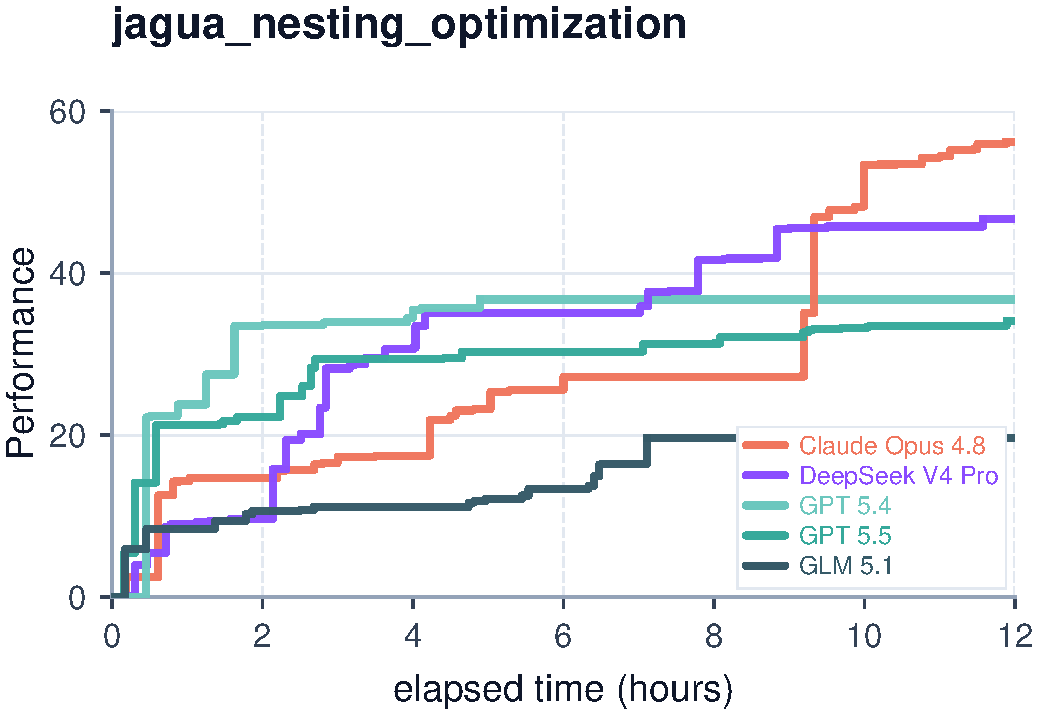
\includegraphics[width=\linewidth]{figures/curves/jagua_nesting_optimizer_time_performance.pdf}
\end{subfigure}
\hfill
\begin{subfigure}[b]{0.48\linewidth}
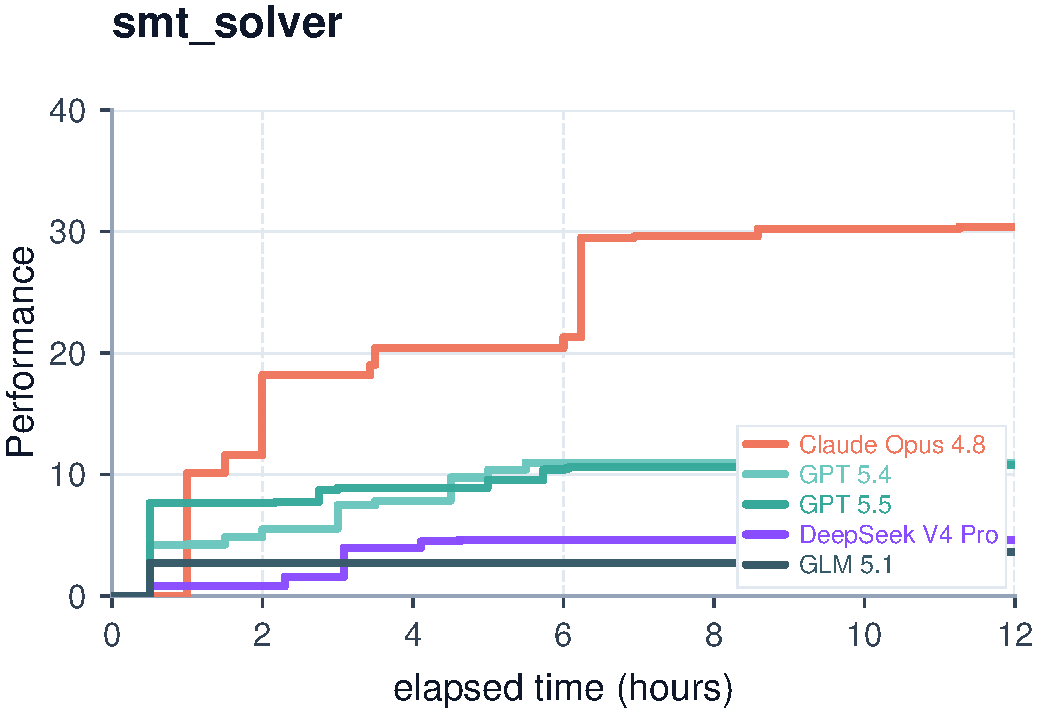
\includegraphics[width=\linewidth]{figures/curves/smt_solver_time_performance.pdf}
\end{subfigure}
\vspace{0.5em}
\begin{subfigure}[b]{0.48\linewidth}
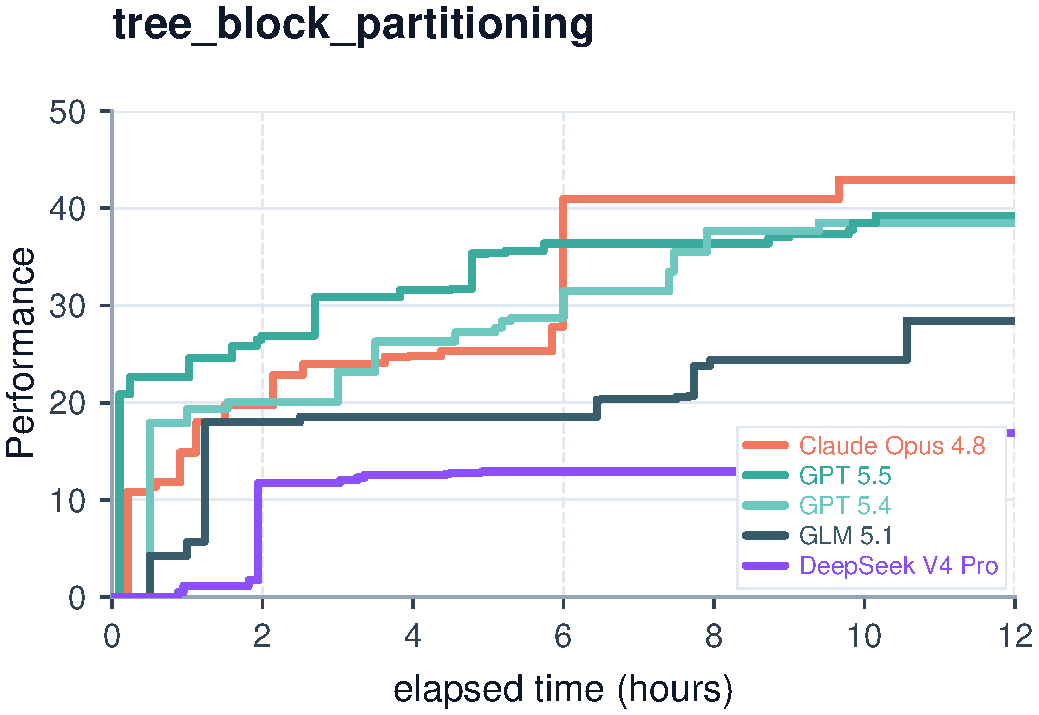
\includegraphics[width=\linewidth]{figures/curves/tree_block_partitioning_time_performance.pdf}
\end{subfigure}
\hfill
\begin{subfigure}[b]{0.48\linewidth}
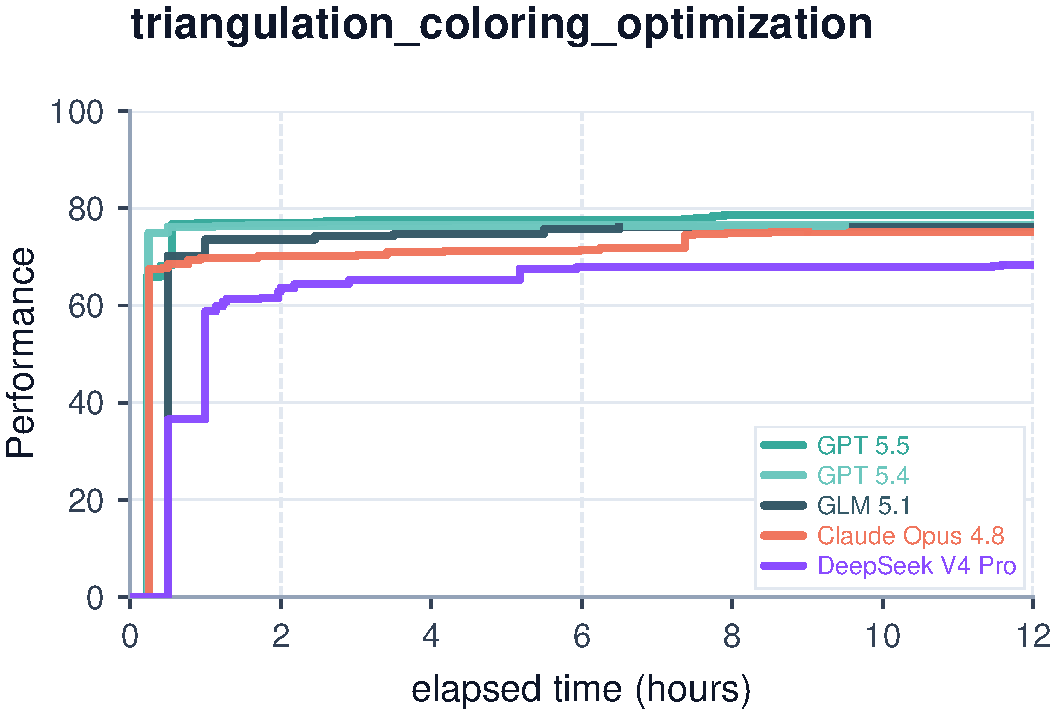
\includegraphics[width=\linewidth]{figures/curves/tricol_time_performance.pdf}
\end{subfigure}
\caption{Per-task learning curves: Combinatorial Optimization \& Planning cont. (14/21).}
\label{fig:curves-all-14}
\end{figure}

\begin{figure}[p]
\centering
\begin{subfigure}[b]{0.48\linewidth}
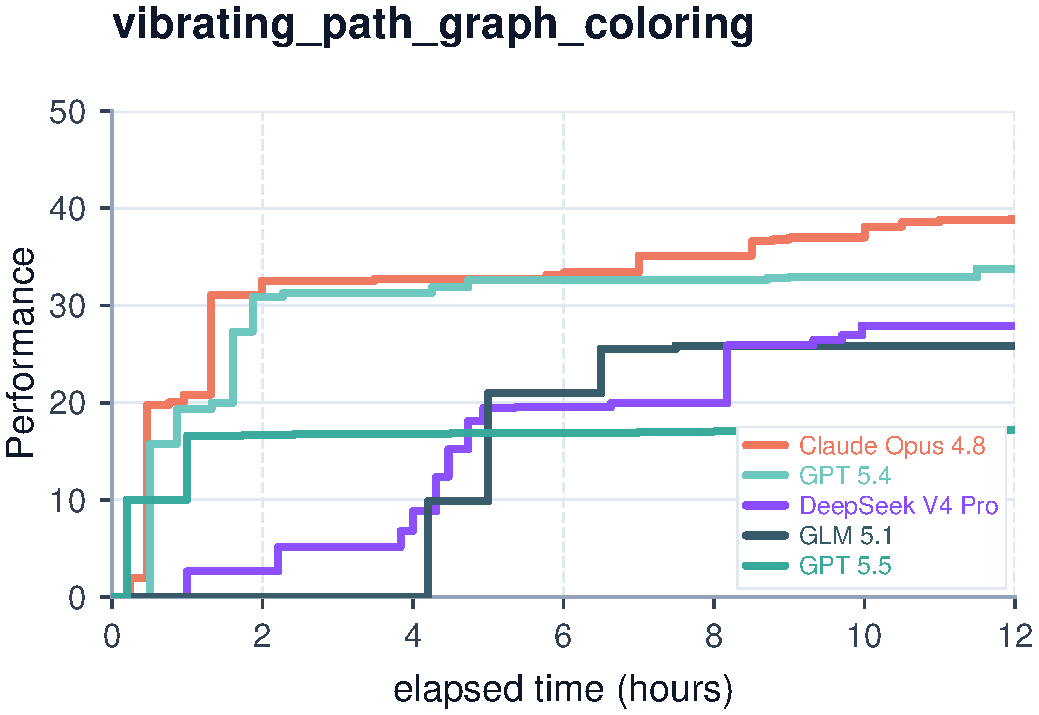
\includegraphics[width=\linewidth]{figures/curves/vbr_time_performance.pdf}
\end{subfigure}
\hfill
\begin{subfigure}[b]{0.48\linewidth}
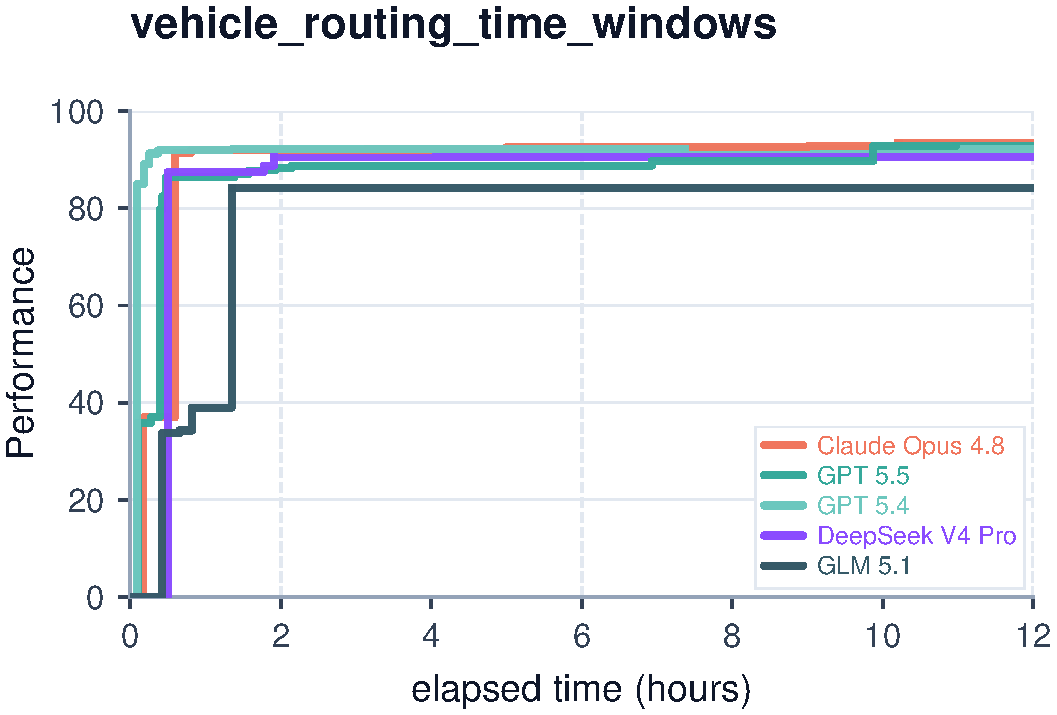
\includegraphics[width=\linewidth]{figures/curves/vehicle_routing_time_windows_time_performance.pdf}
\end{subfigure}
\vspace{0.5em}
\begin{subfigure}[b]{0.48\linewidth}
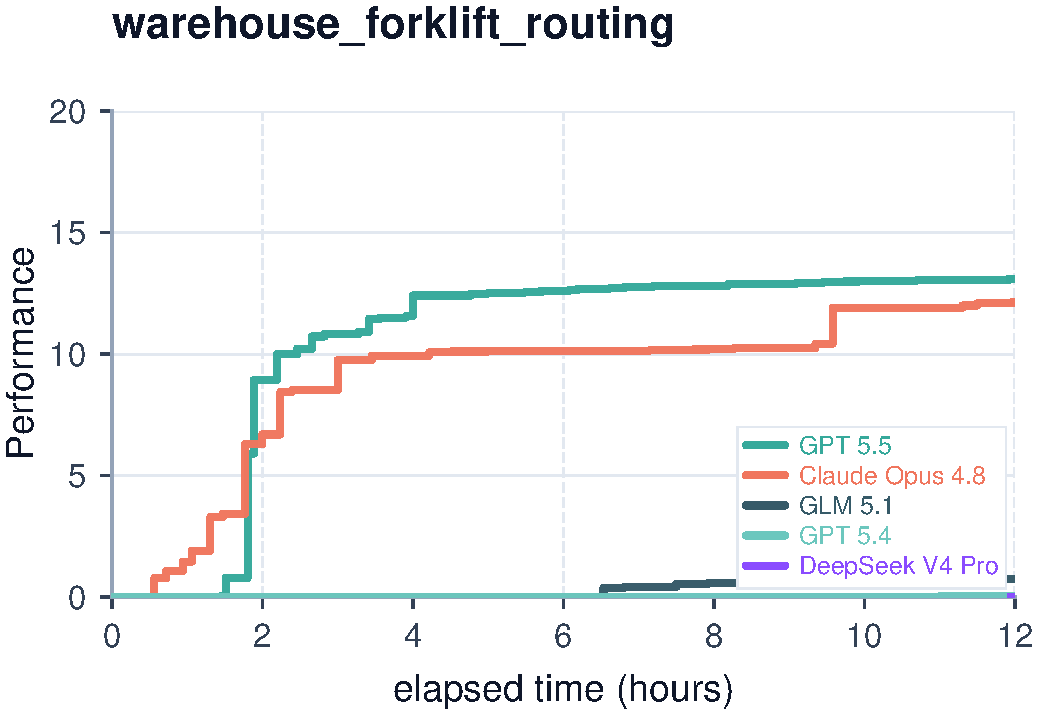
\includegraphics[width=\linewidth]{figures/curves/warehouse_manager_time_performance.pdf}
\end{subfigure}
\hfill
\begin{subfigure}[b]{0.48\linewidth}
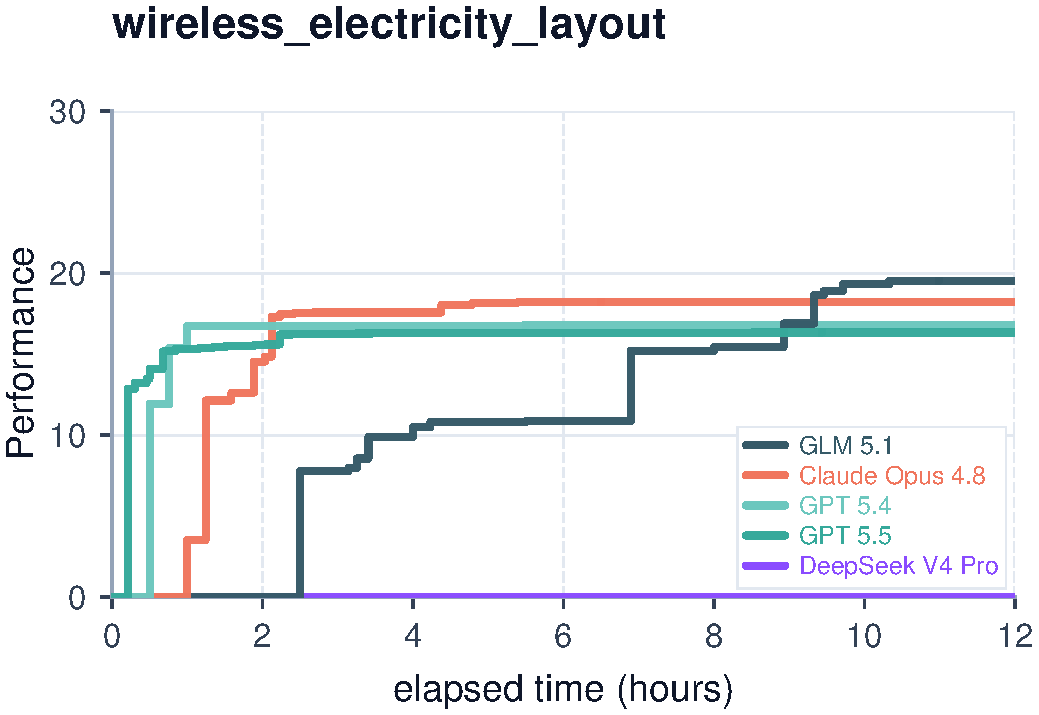
\includegraphics[width=\linewidth]{figures/curves/wirel_time_performance.pdf}
\end{subfigure}
\caption{Per-task learning curves: Combinatorial Optimization \& Planning cont. (15/21).}
\label{fig:curves-all-15}
\end{figure}

\begin{figure}[p]
\centering
\begin{subfigure}[b]{0.48\linewidth}
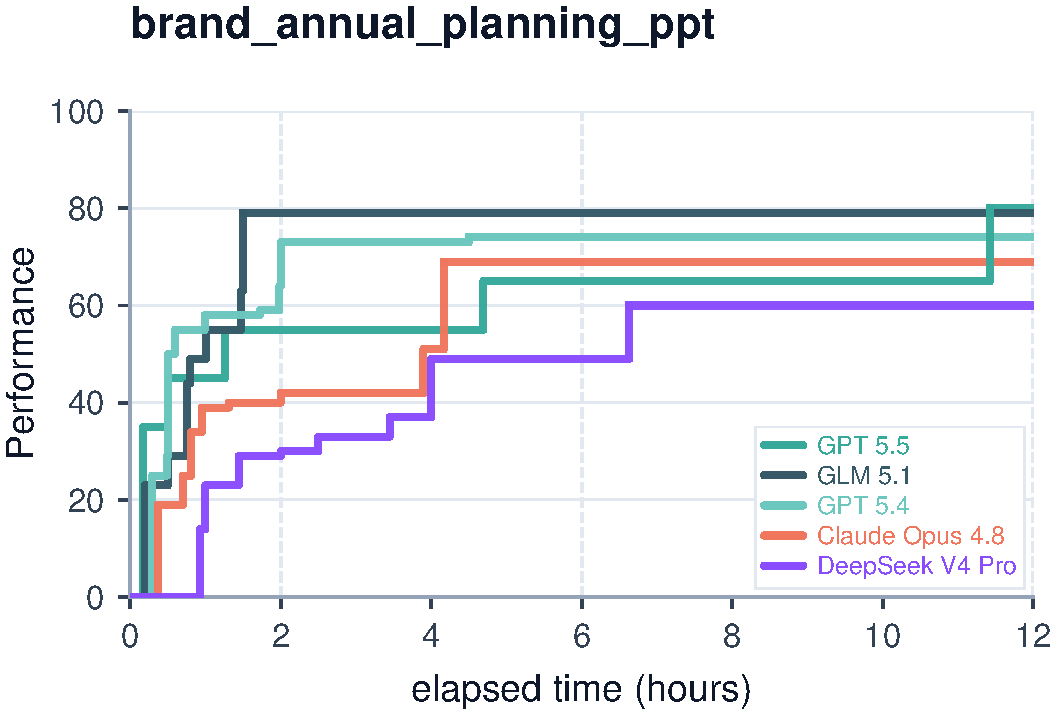
\includegraphics[width=\linewidth]{figures/curves/brand_annual_planning_ppt_time_performance.pdf}
\end{subfigure}
\hfill
\begin{subfigure}[b]{0.48\linewidth}
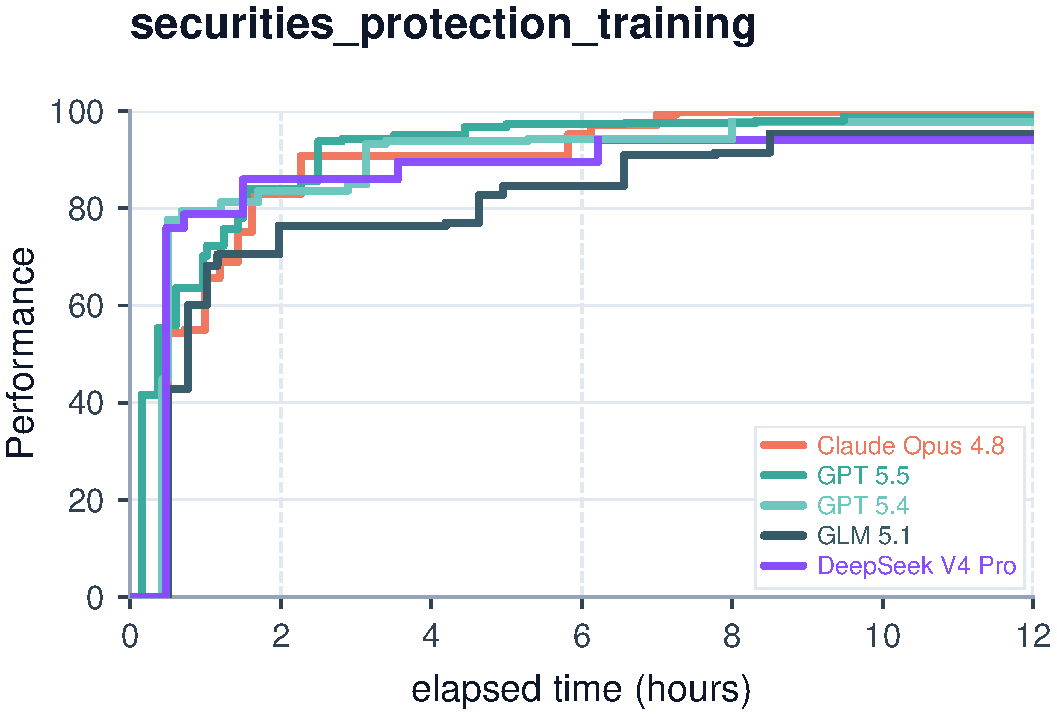
\includegraphics[width=\linewidth]{figures/curves/china_securities_protection_training_time_performance.pdf}
\end{subfigure}
\vspace{0.5em}
\begin{subfigure}[b]{0.48\linewidth}
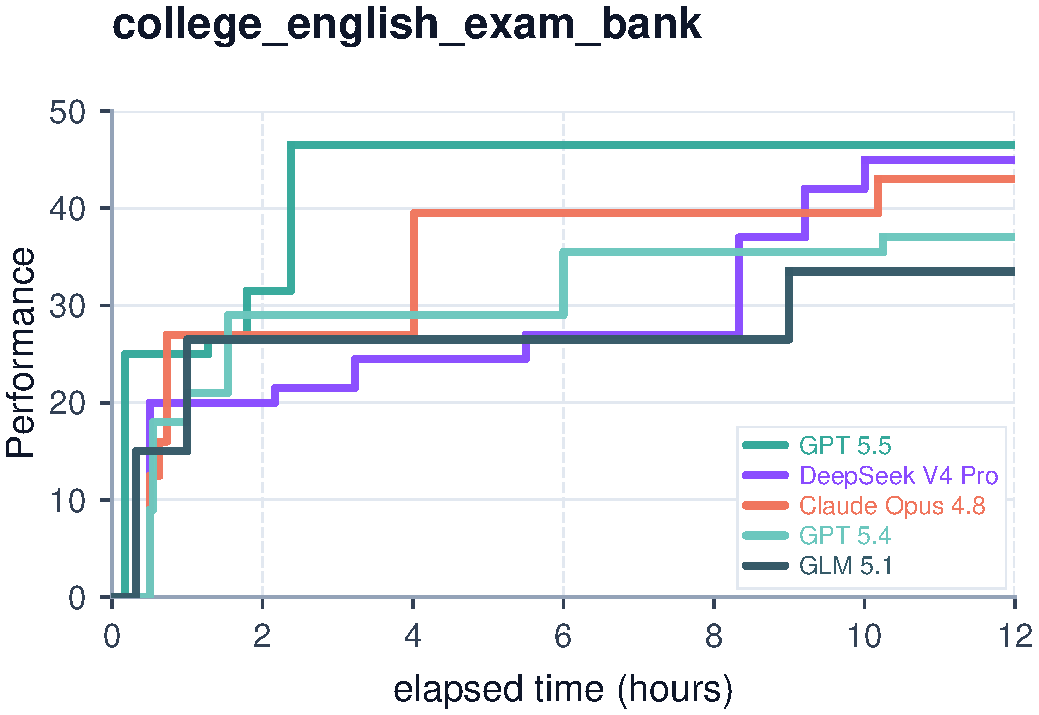
\includegraphics[width=\linewidth]{figures/curves/college_english_exam_bank_time_performance.pdf}
\end{subfigure}
\hfill
\begin{subfigure}[b]{0.48\linewidth}
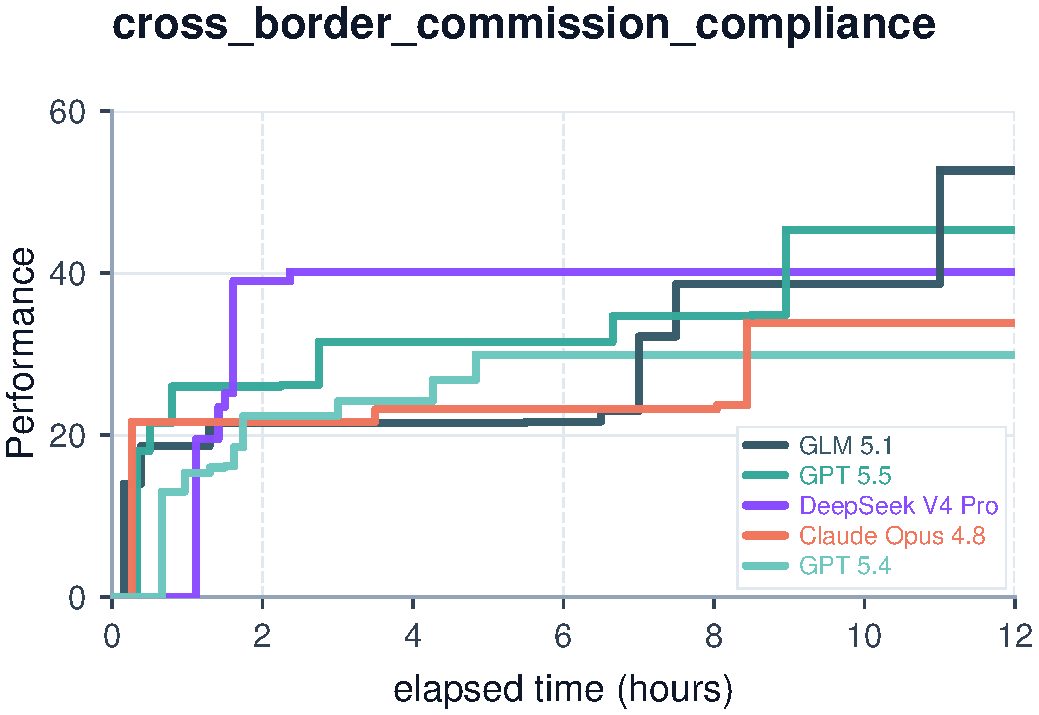
\includegraphics[width=\linewidth]{figures/curves/cross_border_commission_compliance_time_performance.pdf}
\end{subfigure}
\vspace{0.5em}
\begin{subfigure}[b]{0.48\linewidth}
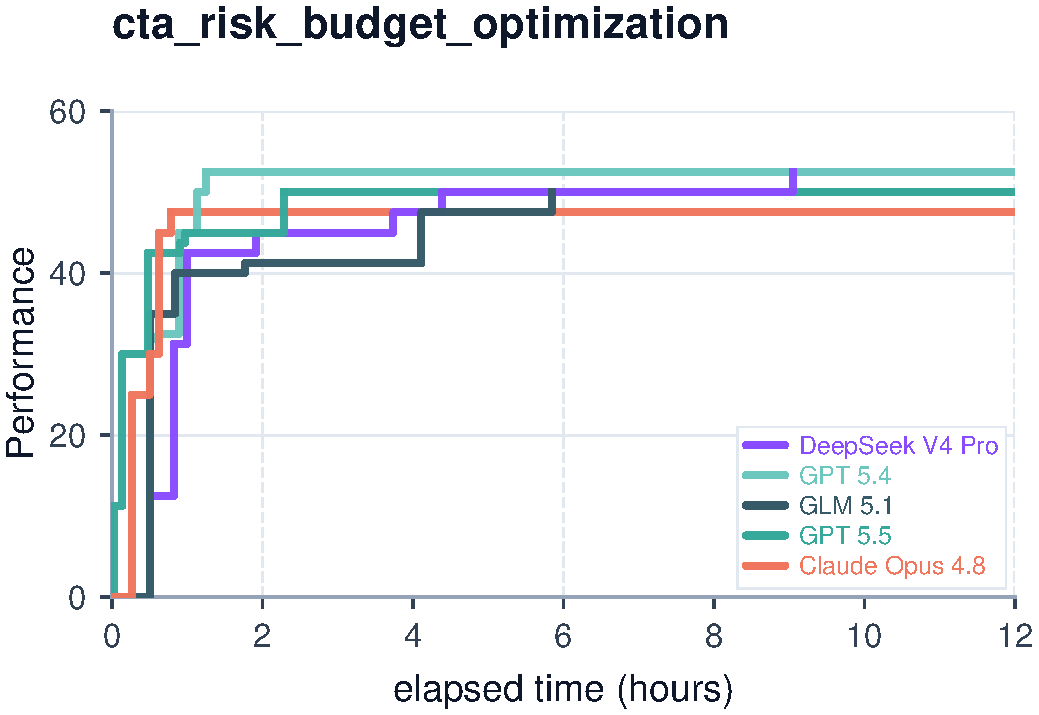
\includegraphics[width=\linewidth]{figures/curves/cta_risk_budget_optimization_time_performance.pdf}
\end{subfigure}
\hfill
\begin{subfigure}[b]{0.48\linewidth}
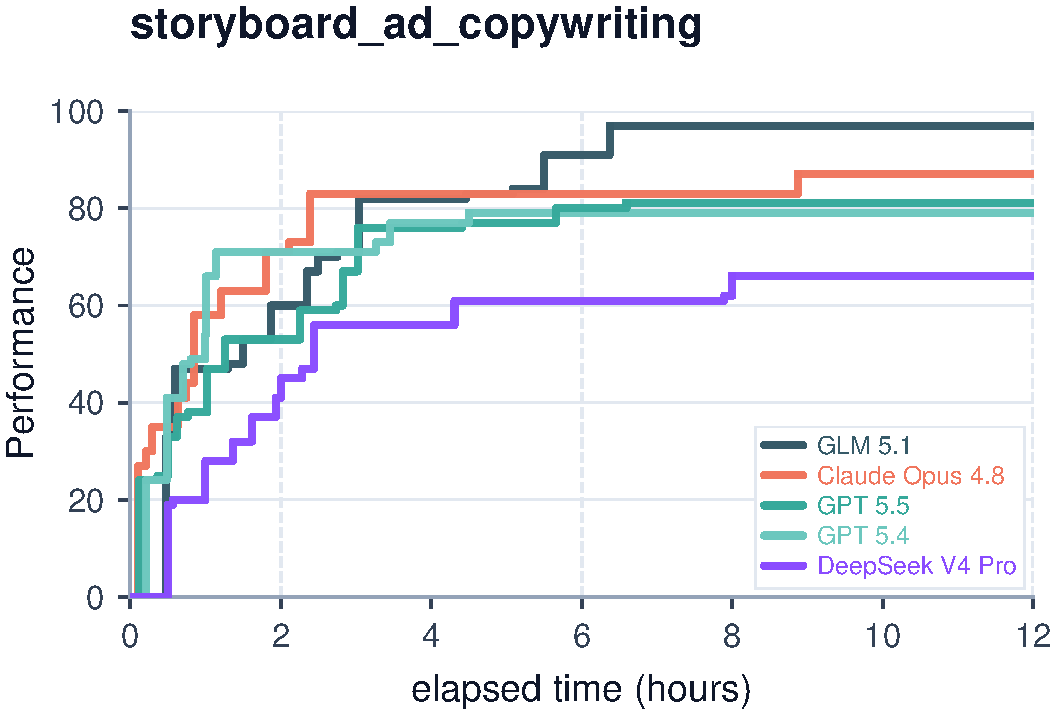
\includegraphics[width=\linewidth]{figures/curves/aigc_storyboard_time_performance.pdf}
\end{subfigure}
\caption{Per-task learning curves: Professional Knowledge Work (16/21).}
\label{fig:curves-all-16}
\end{figure}

\begin{figure}[p]
\centering
\begin{subfigure}[b]{0.48\linewidth}
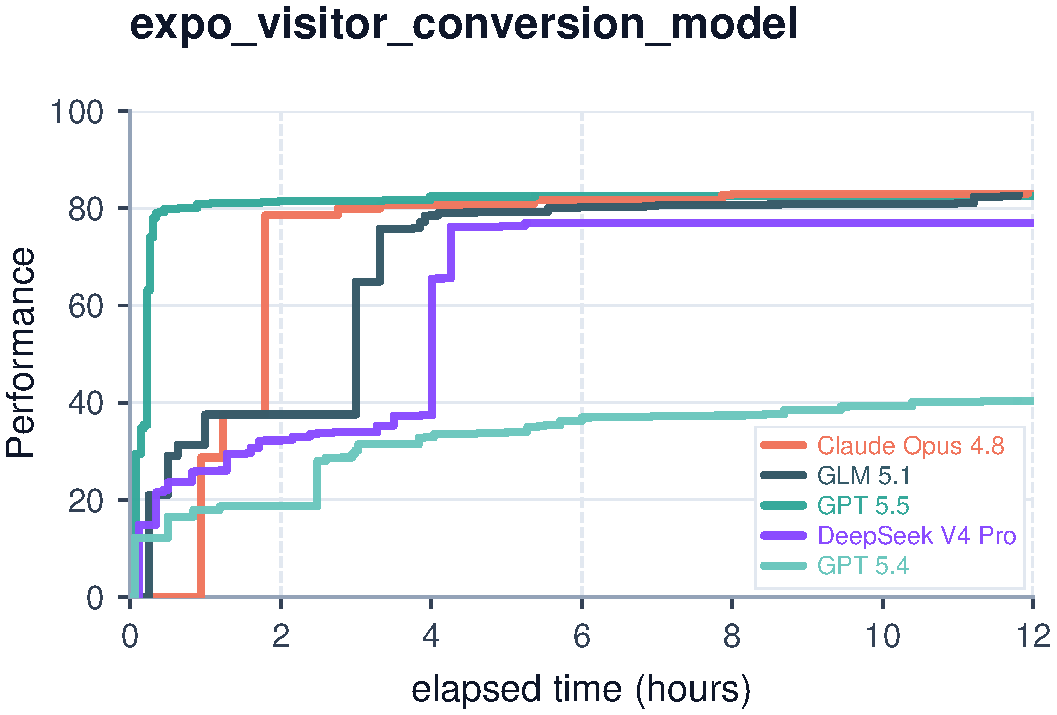
\includegraphics[width=\linewidth]{figures/curves/expo_visitor_cleaning_conversion_model_time_performance.pdf}
\end{subfigure}
\hfill
\begin{subfigure}[b]{0.48\linewidth}
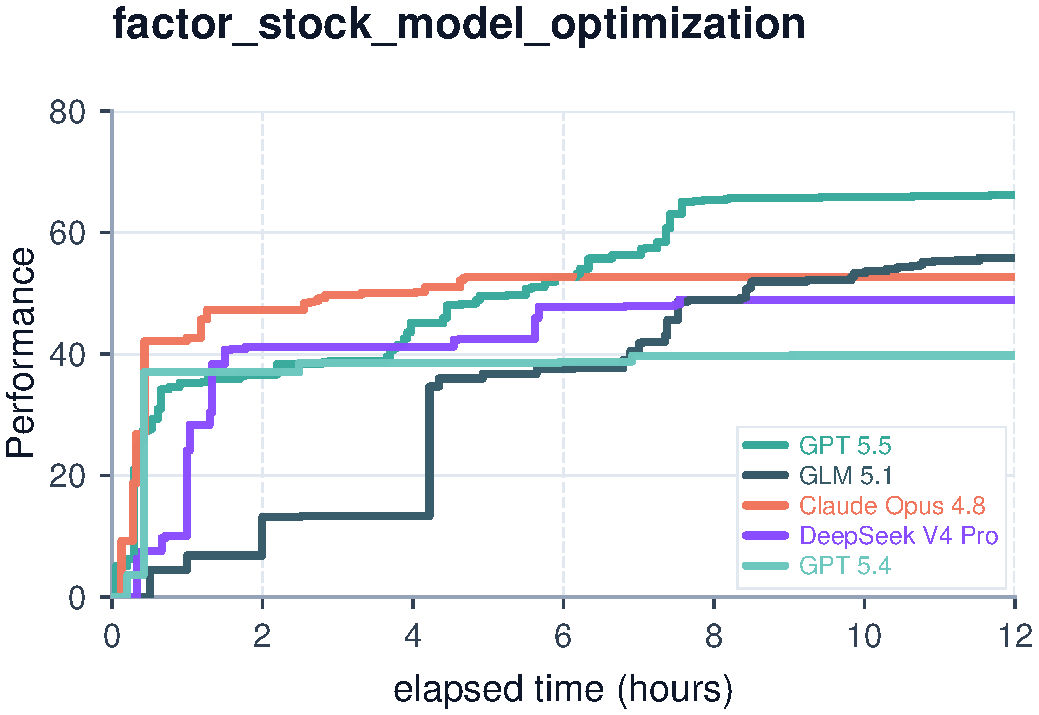
\includegraphics[width=\linewidth]{figures/curves/factor_stock_model_dev_opt_time_performance.pdf}
\end{subfigure}
\vspace{0.5em}
\begin{subfigure}[b]{0.48\linewidth}
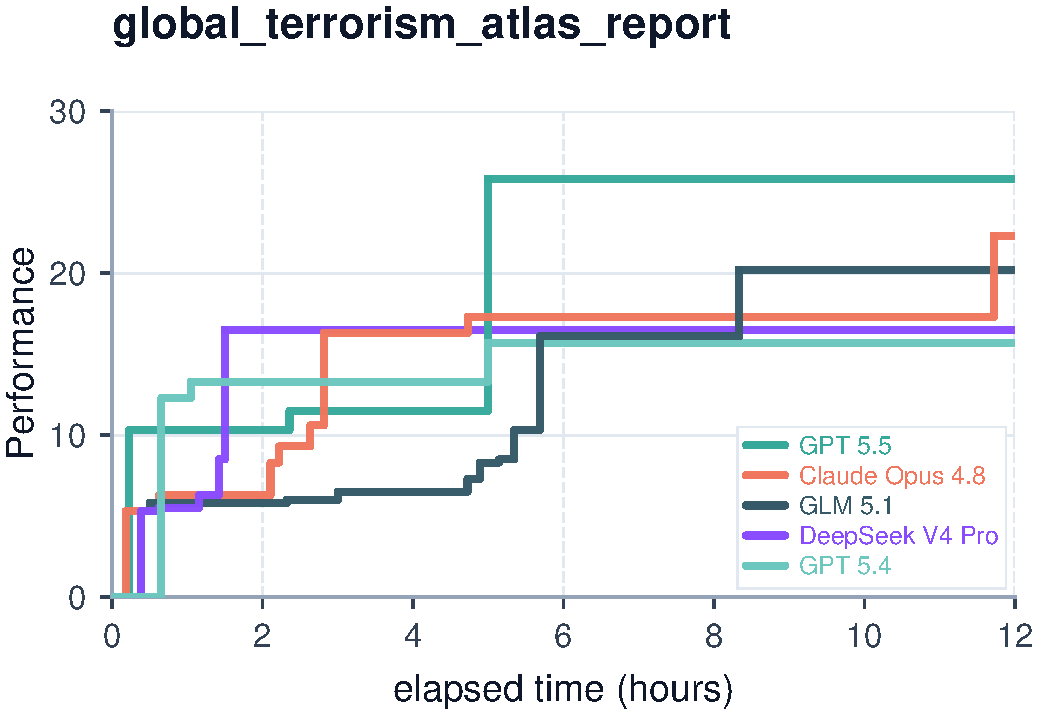
\includegraphics[width=\linewidth]{figures/curves/global_terrorism_atlas_1970_2019_time_performance.pdf}
\end{subfigure}
\hfill
\begin{subfigure}[b]{0.48\linewidth}
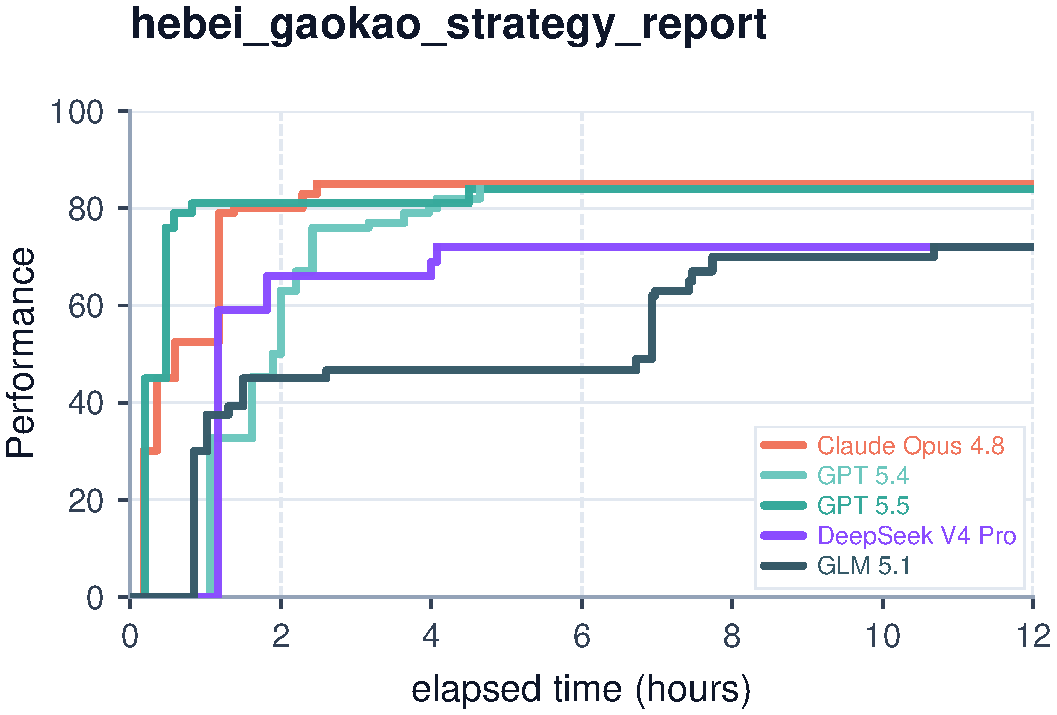
\includegraphics[width=\linewidth]{figures/curves/hebei_gaokao_preference_strategy_time_performance.pdf}
\end{subfigure}
\vspace{0.5em}
\begin{subfigure}[b]{0.48\linewidth}
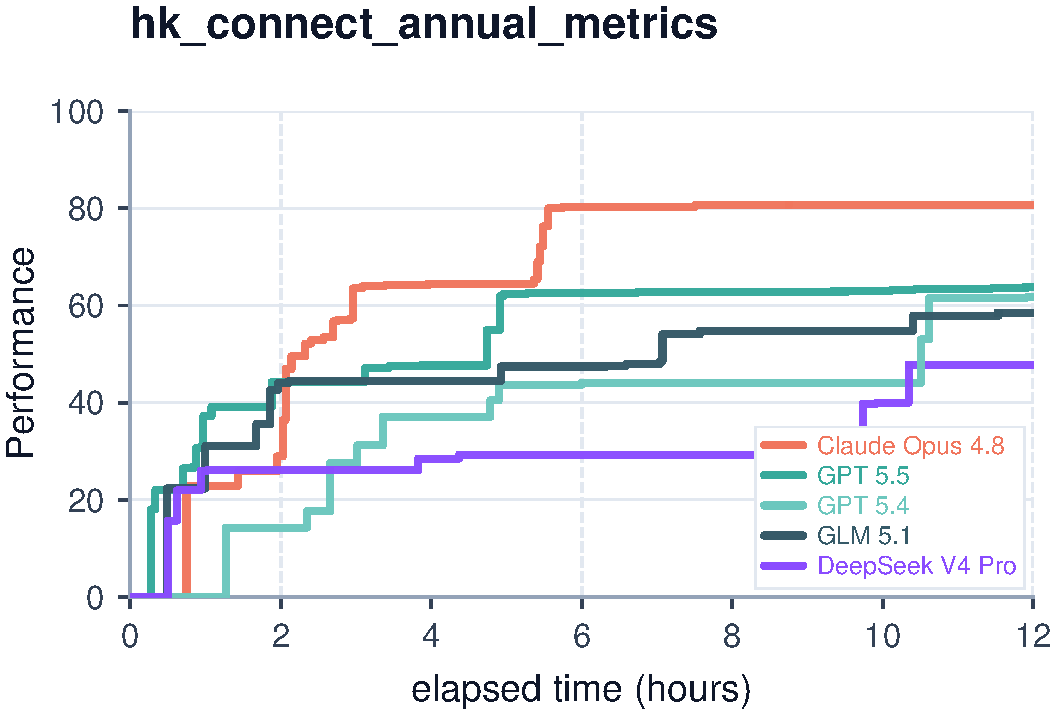
\includegraphics[width=\linewidth]{figures/curves/hk_connect_annual_metrics_time_performance.pdf}
\end{subfigure}
\hfill
\begin{subfigure}[b]{0.48\linewidth}
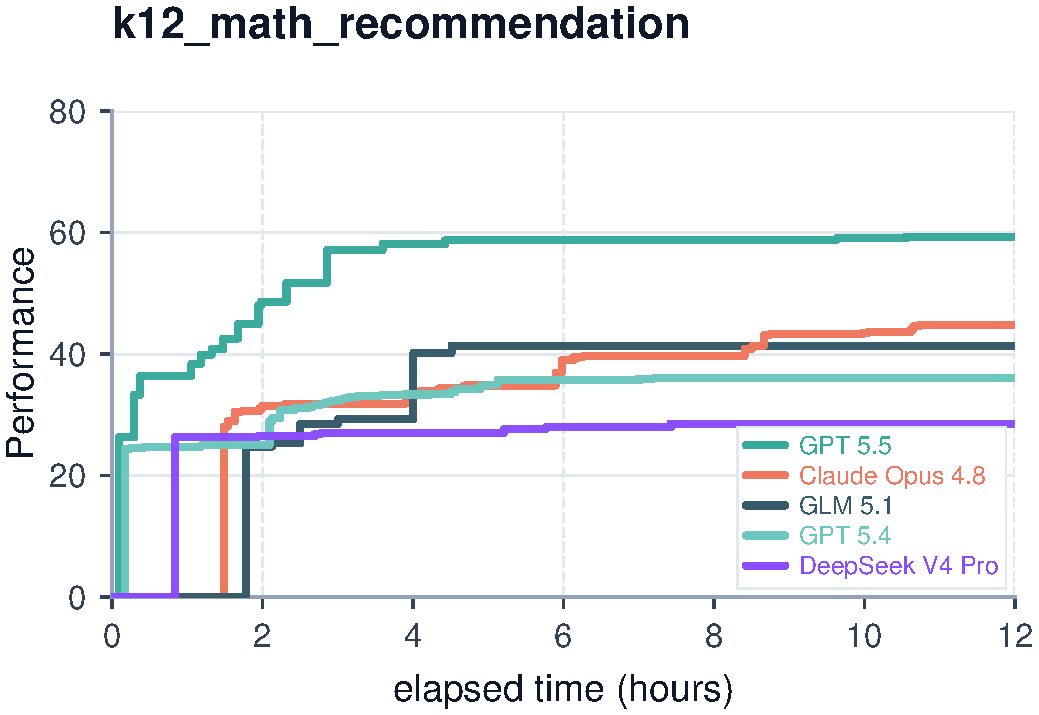
\includegraphics[width=\linewidth]{figures/curves/k12_math_recommendation_time_performance.pdf}
\end{subfigure}
\caption{Per-task learning curves: Professional Knowledge Work cont. (17/21).}
\label{fig:curves-all-17}
\end{figure}

\begin{figure}[p]
\centering
\begin{subfigure}[b]{0.48\linewidth}
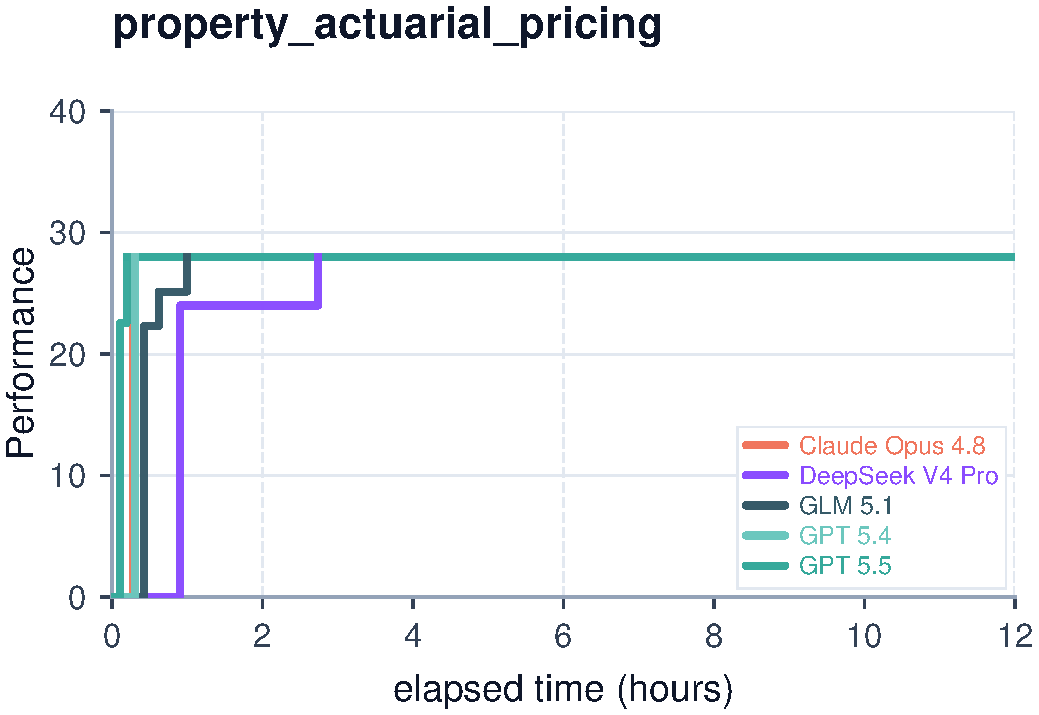
\includegraphics[width=\linewidth]{figures/curves/property_actuarial_pricing_time_performance.pdf}
\end{subfigure}
\hfill
\begin{subfigure}[b]{0.48\linewidth}
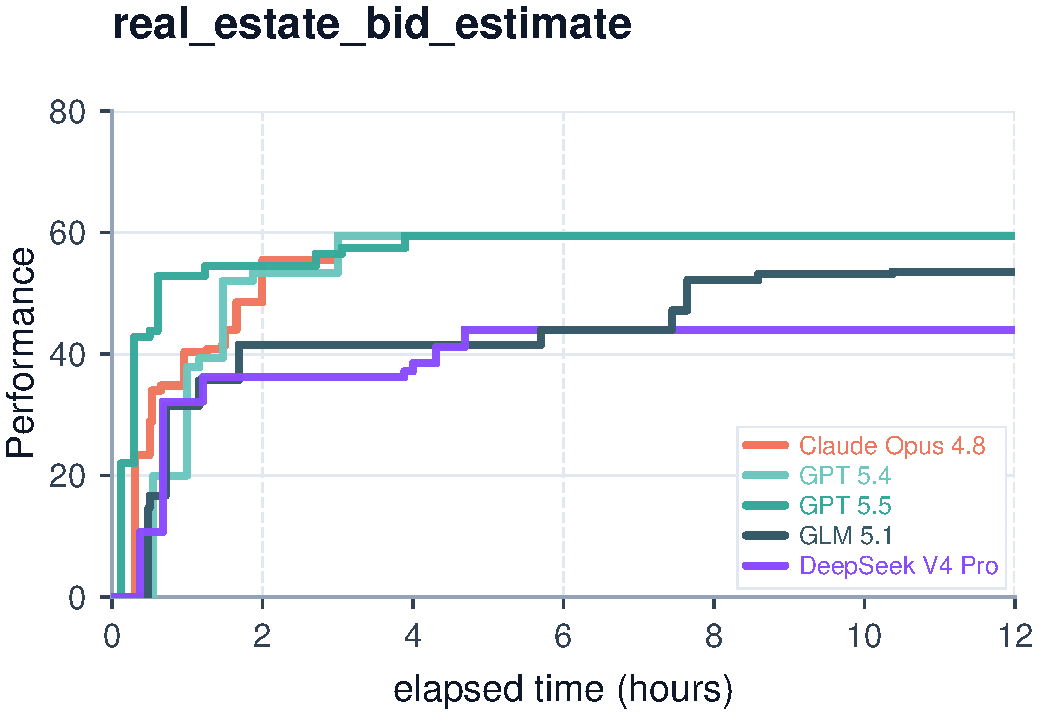
\includegraphics[width=\linewidth]{figures/curves/real_estate_bid_economic_estimate_time_performance.pdf}
\end{subfigure}
\vspace{0.5em}
\begin{subfigure}[b]{0.48\linewidth}
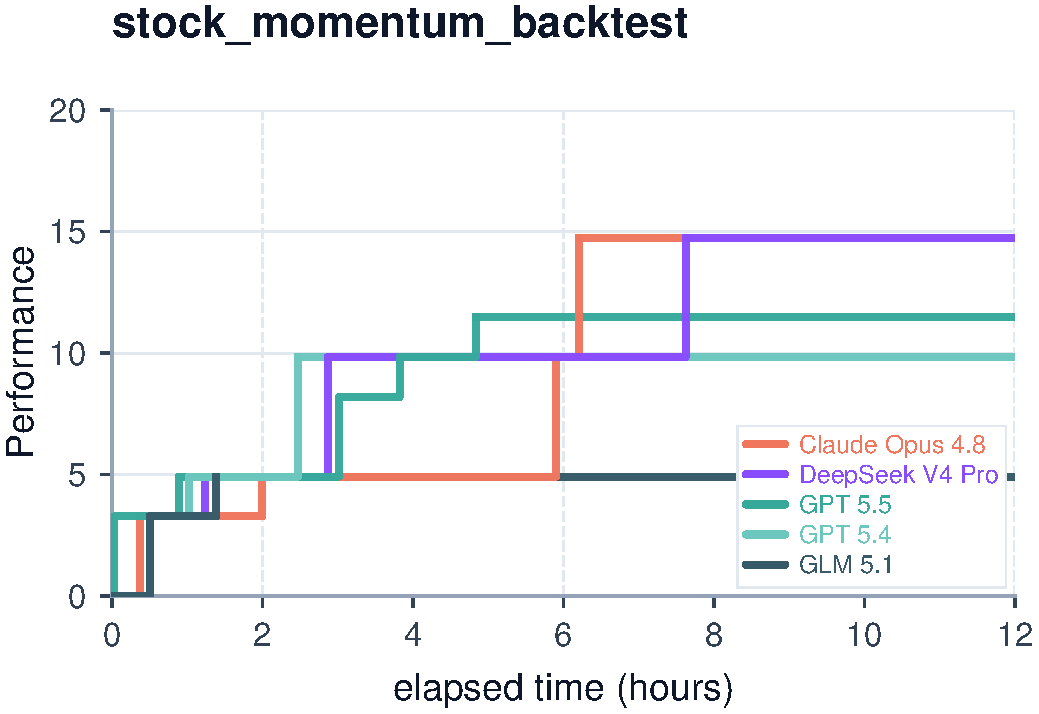
\includegraphics[width=\linewidth]{figures/curves/share_momentum_return_backtest_time_performance.pdf}
\end{subfigure}
\hfill
\begin{subfigure}[b]{0.48\linewidth}
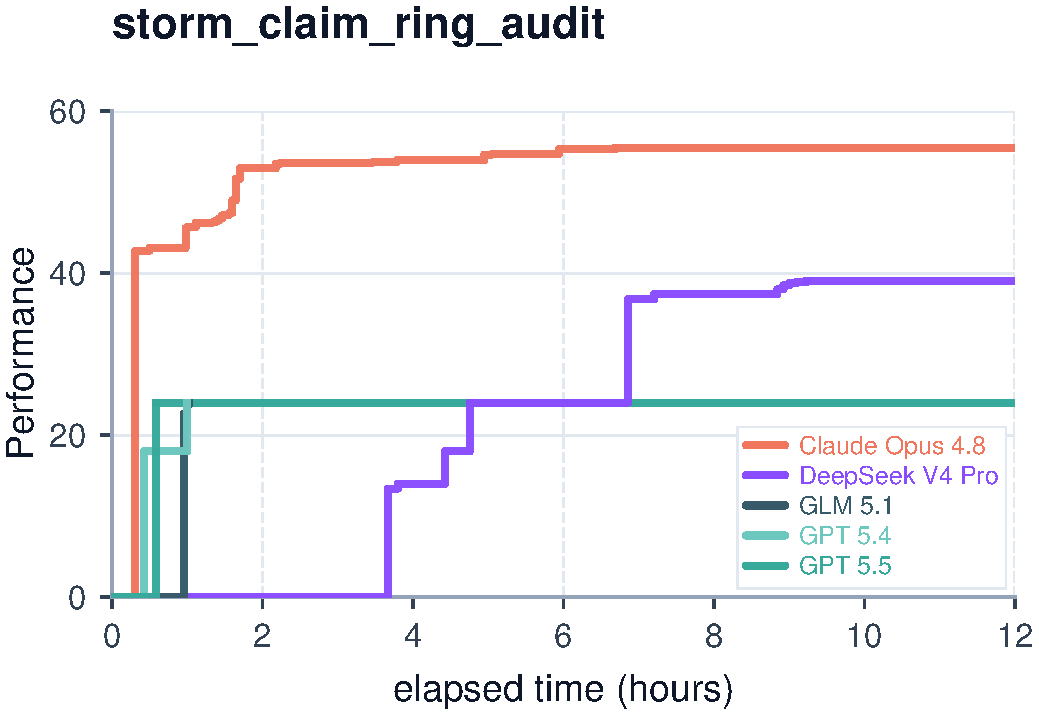
\includegraphics[width=\linewidth]{figures/curves/storm_claim_ring_audit_time_performance.pdf}
\end{subfigure}
\caption{Per-task learning curves: Professional Knowledge Work cont. (18/21).}
\label{fig:curves-all-18}
\end{figure}

\begin{figure}[p]
\centering
\begin{subfigure}[b]{0.48\linewidth}
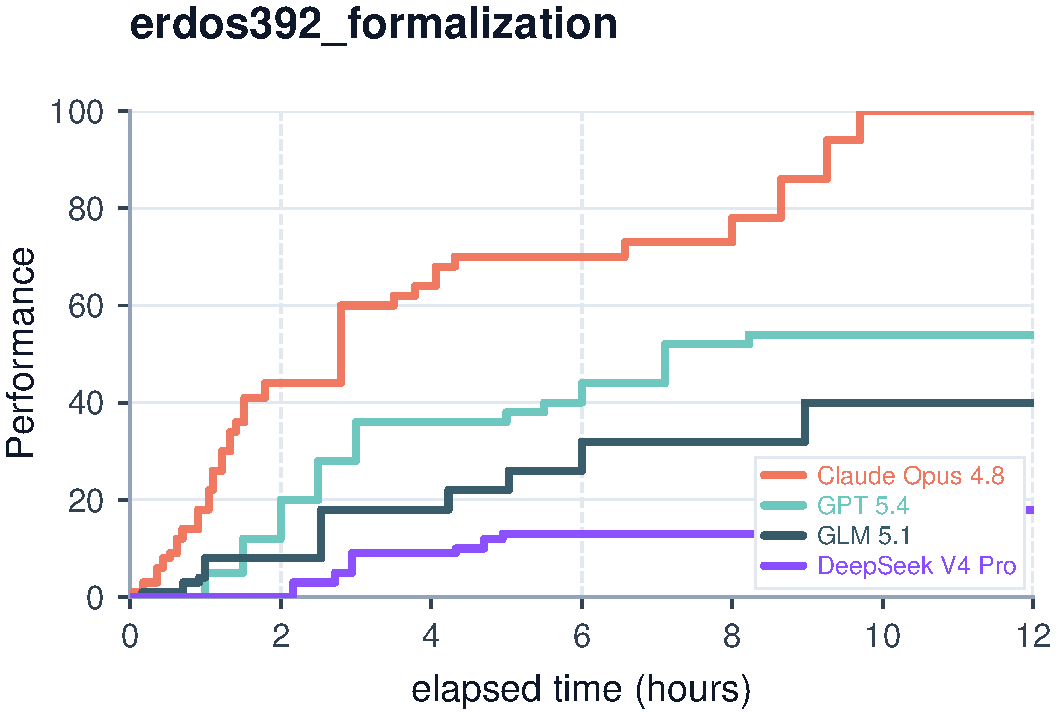
\includegraphics[width=\linewidth]{figures/curves/erdos392_time_performance.pdf}
\end{subfigure}
\hfill
\begin{subfigure}[b]{0.48\linewidth}
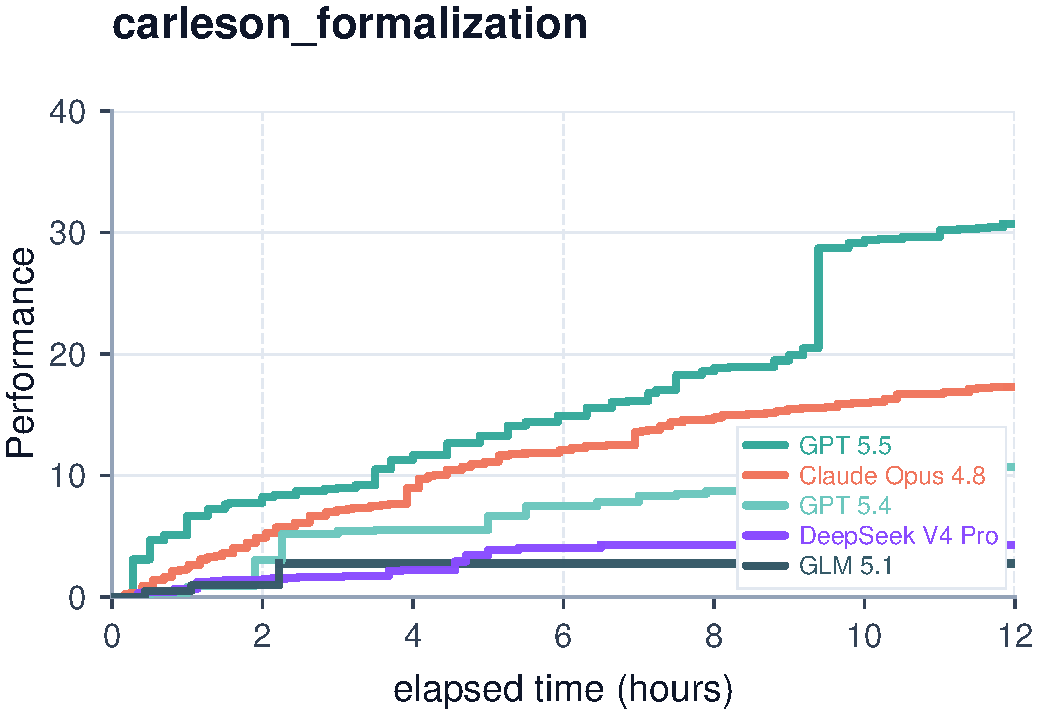
\includegraphics[width=\linewidth]{figures/curves/carleson_time_performance.pdf}
\end{subfigure}
\vspace{0.5em}
\begin{subfigure}[b]{0.48\linewidth}
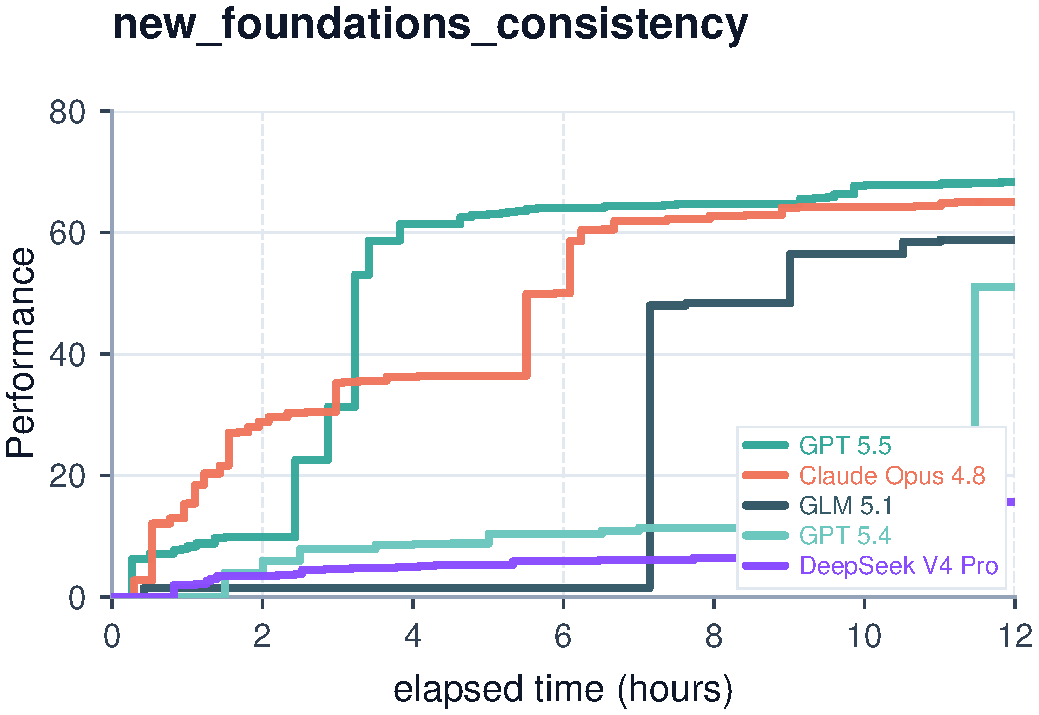
\includegraphics[width=\linewidth]{figures/curves/connf_time_performance.pdf}
\end{subfigure}
\hfill
\begin{subfigure}[b]{0.48\linewidth}
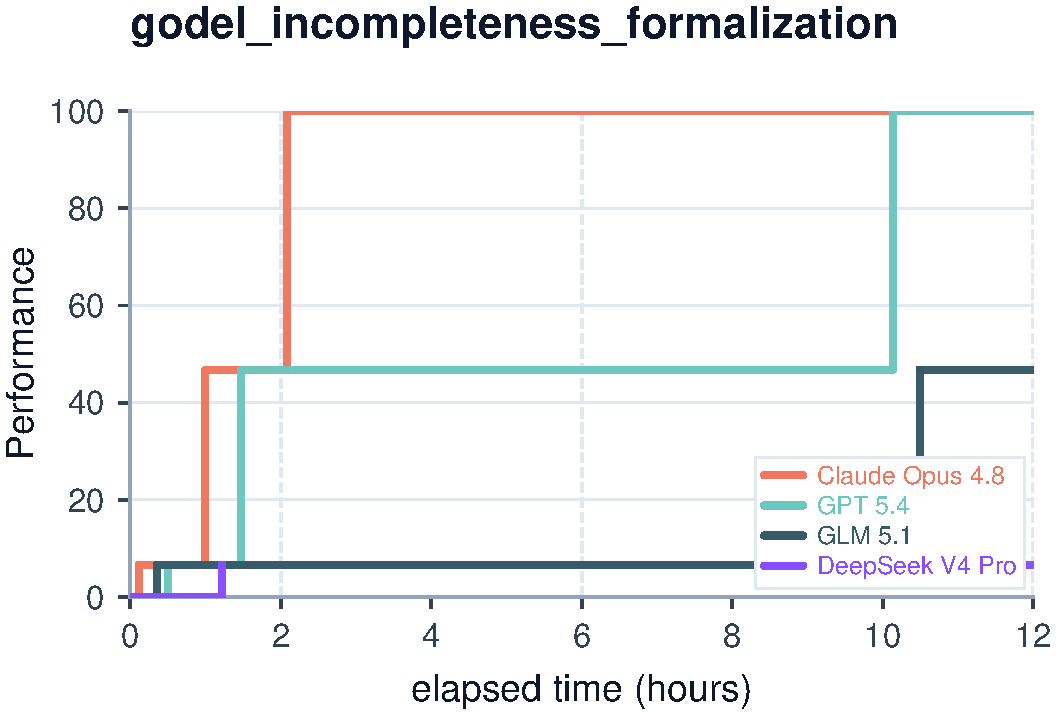
\includegraphics[width=\linewidth]{figures/curves/incomplete_time_performance.pdf}
\end{subfigure}
\vspace{0.5em}
\begin{subfigure}[b]{0.48\linewidth}
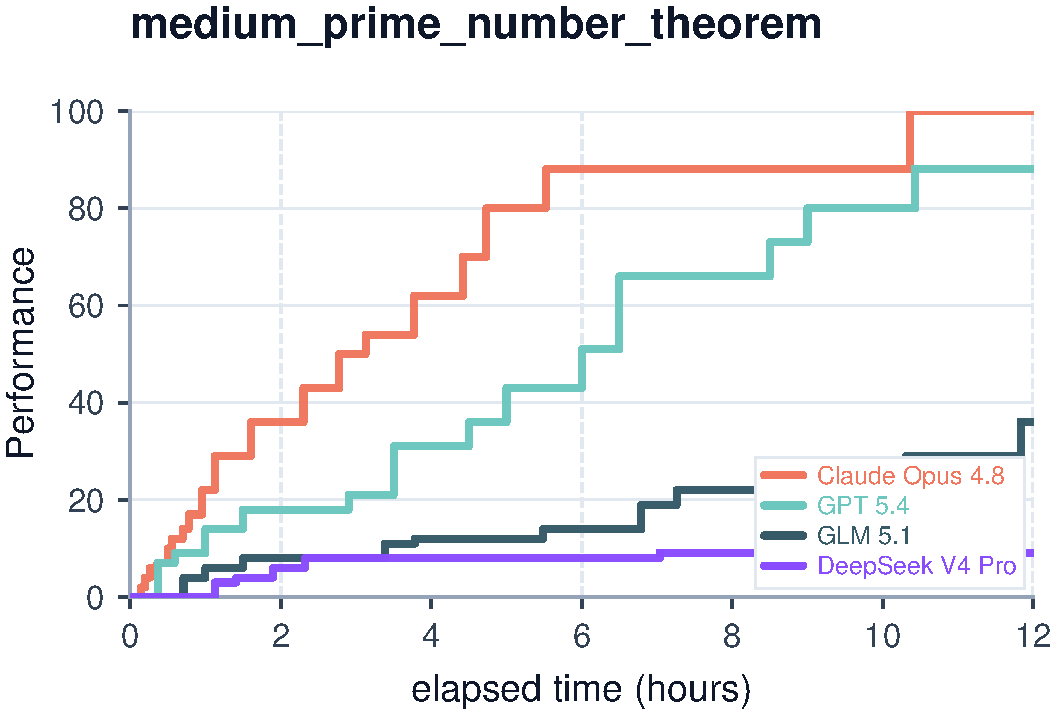
\includegraphics[width=\linewidth]{figures/curves/midpnt_time_performance.pdf}
\end{subfigure}
\hfill
\begin{subfigure}[b]{0.48\linewidth}
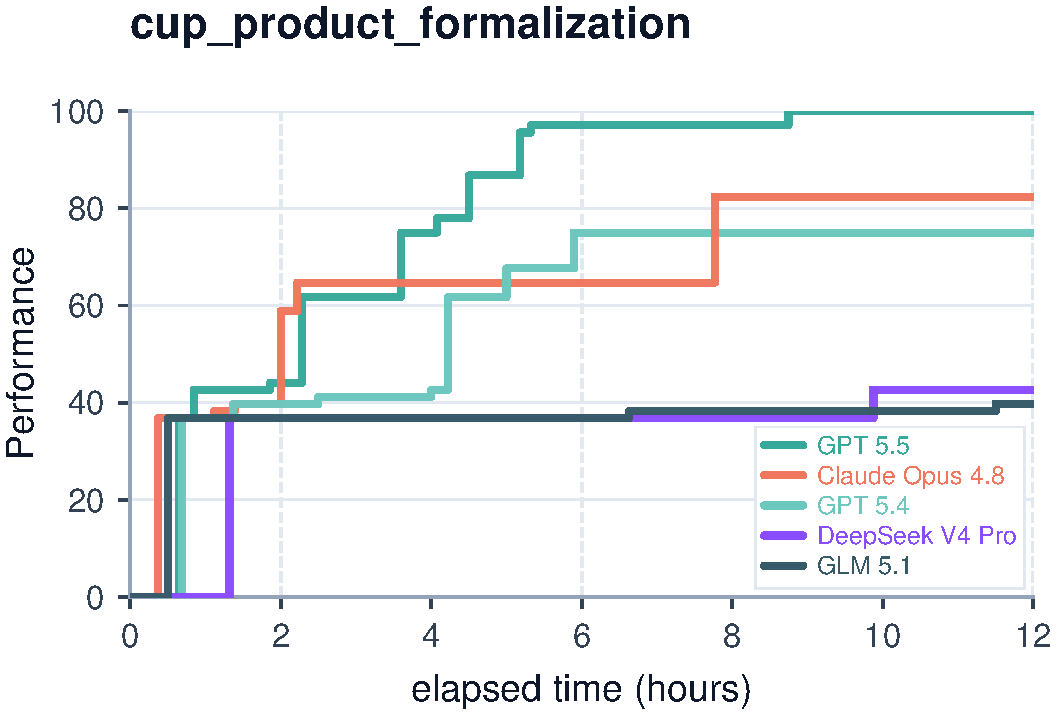
\includegraphics[width=\linewidth]{figures/curves/cup_time_performance.pdf}
\end{subfigure}
\caption{Per-task learning curves: Formal Math \& Theorem Proving (19/21).}
\label{fig:curves-all-19}
\end{figure}

\begin{figure}[p]
\centering
\begin{subfigure}[b]{0.48\linewidth}
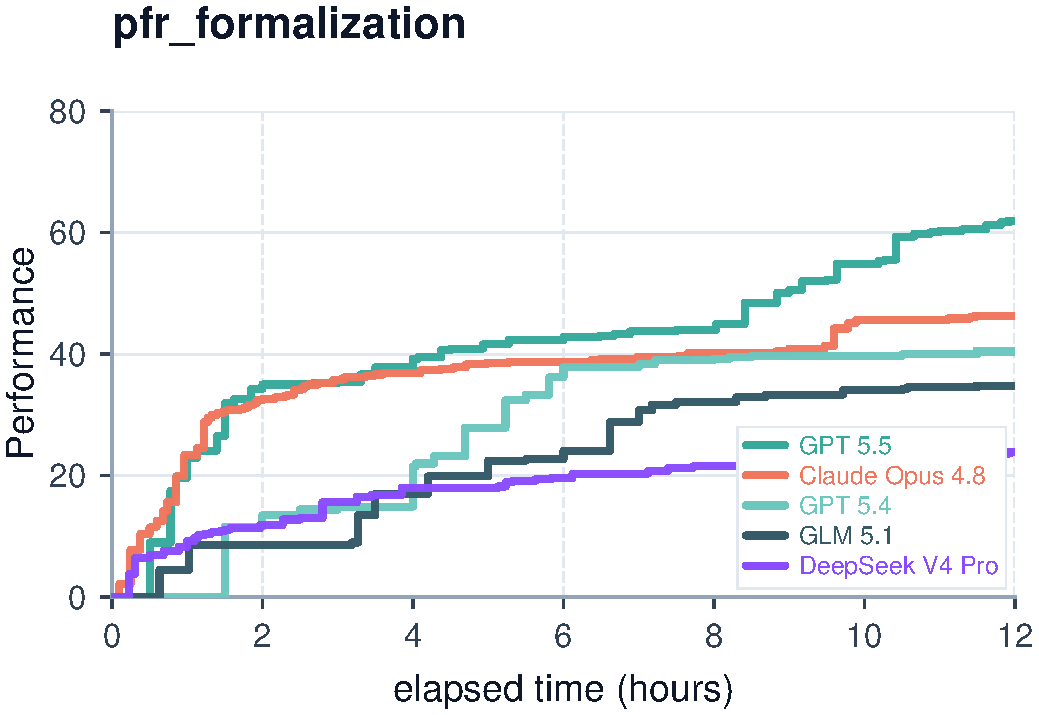
\includegraphics[width=\linewidth]{figures/curves/pfr_time_performance.pdf}
\end{subfigure}
\hfill
\begin{subfigure}[b]{0.48\linewidth}
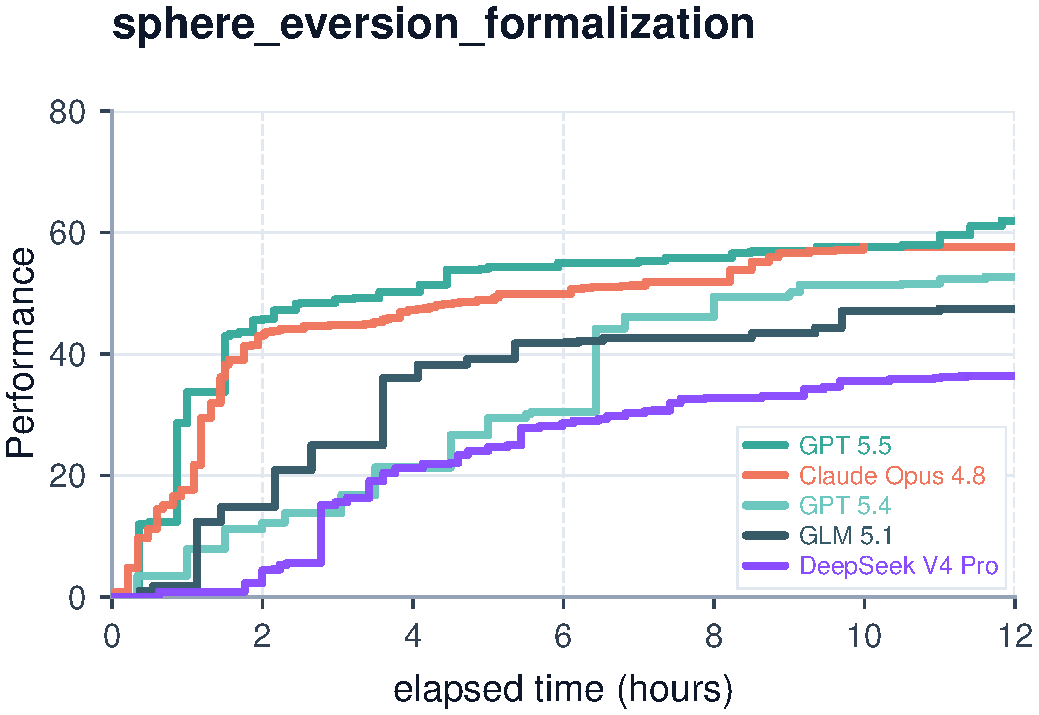
\includegraphics[width=\linewidth]{figures/curves/sphere_time_performance.pdf}
\end{subfigure}
\vspace{0.5em}
\begin{subfigure}[b]{0.48\linewidth}
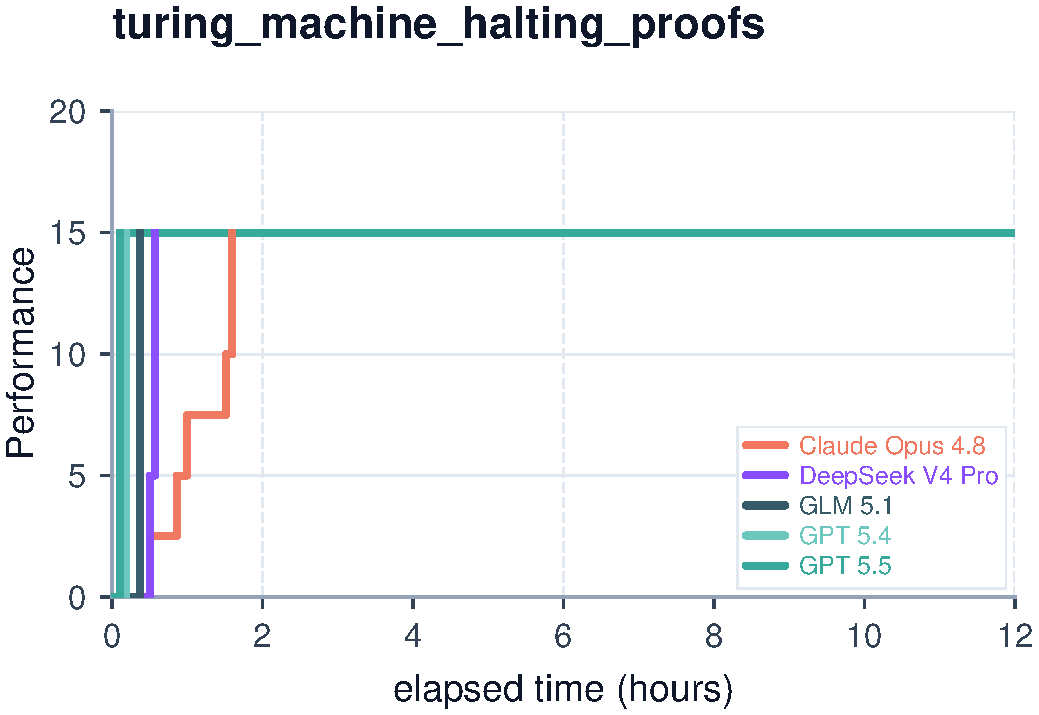
\includegraphics[width=\linewidth]{figures/curves/tm6x2_time_performance.pdf}
\end{subfigure}
\hfill
\begin{subfigure}[b]{0.48\linewidth}
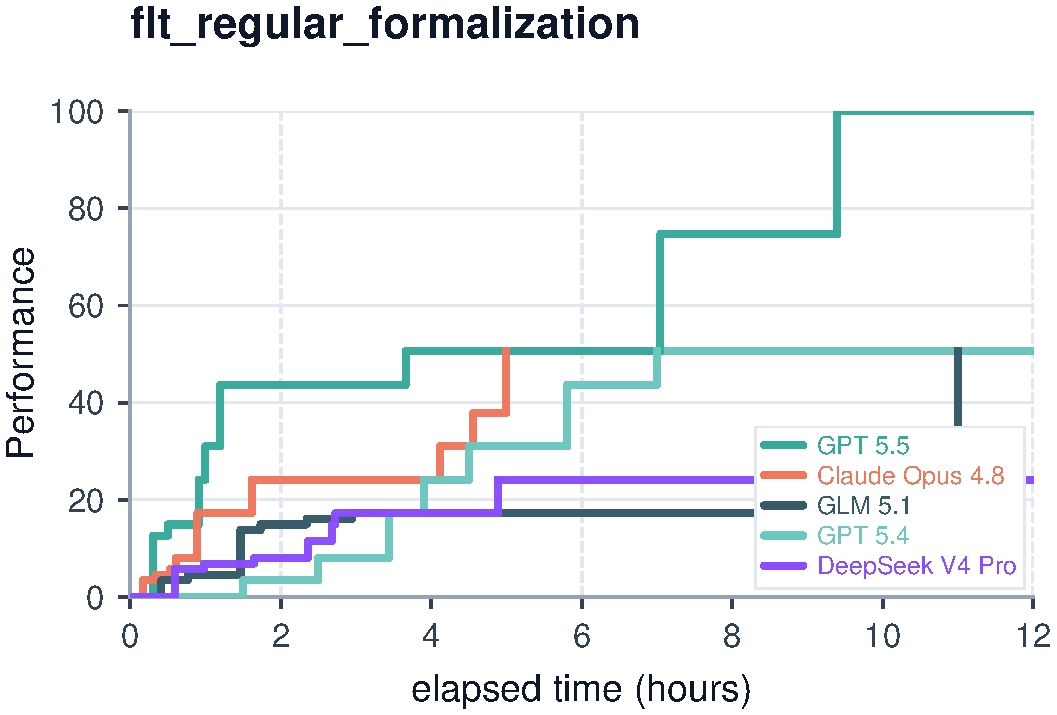
\includegraphics[width=\linewidth]{figures/curves/fltregular_time_performance.pdf}
\end{subfigure}
\caption{Per-task learning curves: Formal Math \& Theorem Proving cont. (20/21).}
\label{fig:curves-all-20}
\end{figure}

\begin{figure}[p]
\centering
\begin{subfigure}[b]{0.48\linewidth}
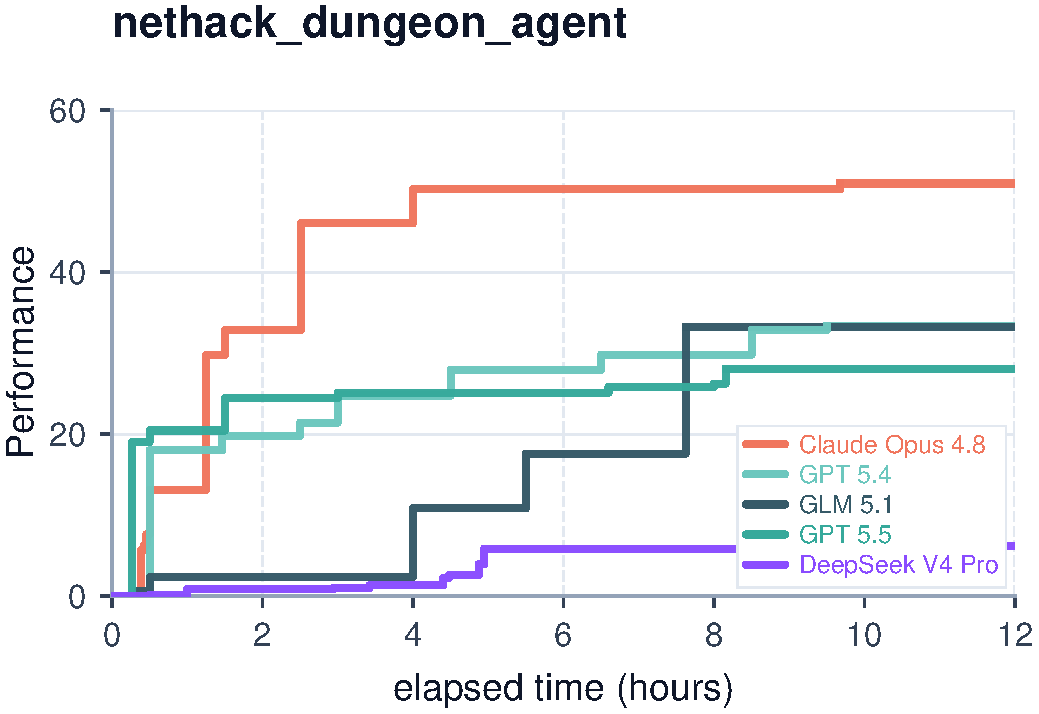
\includegraphics[width=\linewidth]{figures/curves/nethack_time_performance.pdf}
\end{subfigure}
\hfill
\begin{subfigure}[b]{0.48\linewidth}
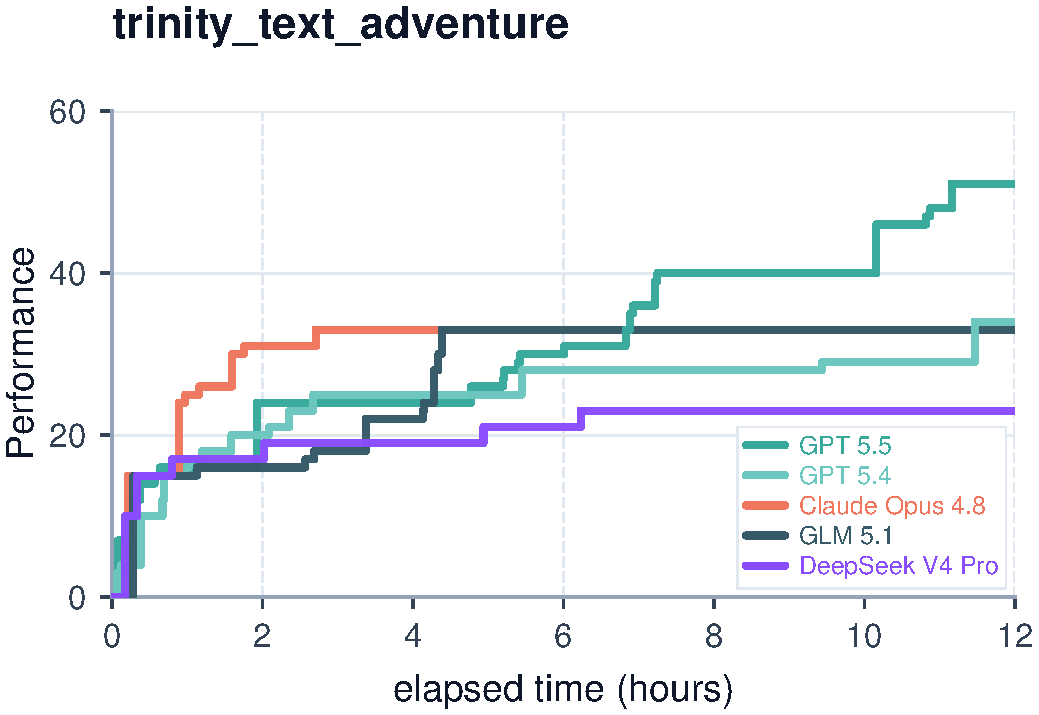
\includegraphics[width=\linewidth]{figures/curves/jericho_trinity_time_performance.pdf}
\end{subfigure}
\vspace{0.5em}
\begin{subfigure}[b]{0.48\linewidth}
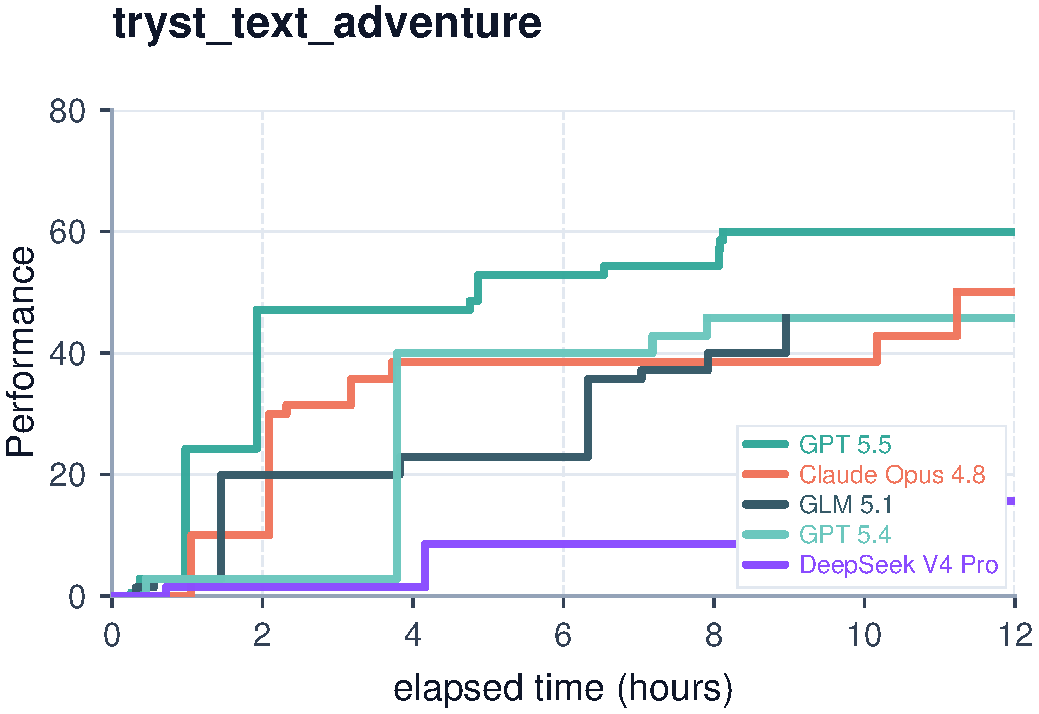
\includegraphics[width=\linewidth]{figures/curves/jericho_tryst_time_performance.pdf}
\end{subfigure}
\hfill
\begin{subfigure}[b]{0.48\linewidth}
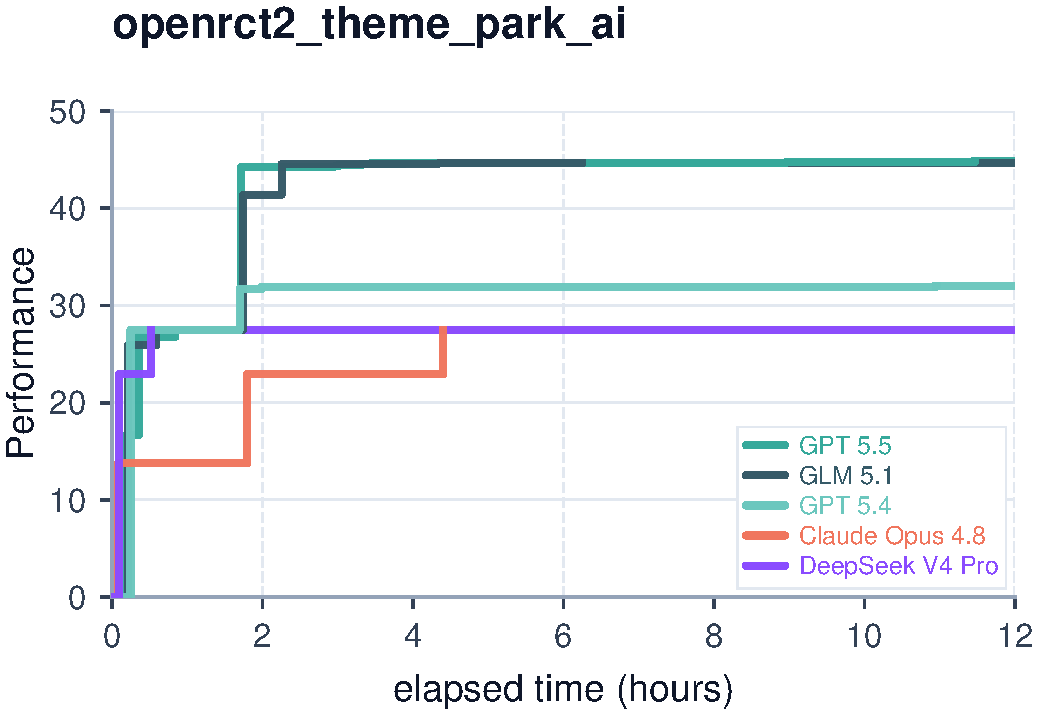
\includegraphics[width=\linewidth]{figures/curves/openrct2_time_performance.pdf}
\end{subfigure}
\vspace{0.5em}
\begin{subfigure}[b]{0.48\linewidth}
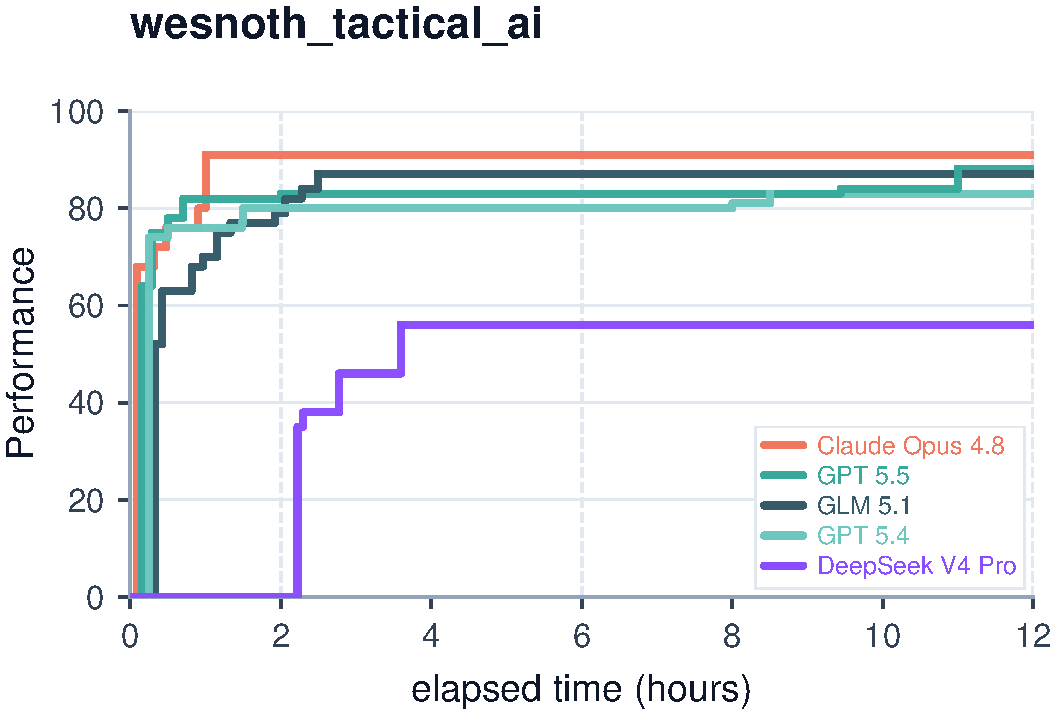
\includegraphics[width=\linewidth]{figures/curves/wesnoth_time_performance.pdf}
\end{subfigure}
\caption{Per-task learning curves: Interactive Games \& Simulators (21/21).}
\label{fig:curves-all-21}
\end{figure}

\clearpage

\subsection{Per-Task Score Tables}
\label{sec:appendix-category-scores}

For every task--model configuration, we scheduled three independent long-horizon runs. In practice, because these 12-hour trajectories are sensitive to network instability and serving-side reliability limits, we carried out multiple rolling evaluation rounds to recover failed or incomplete runs and produced the final score tables below. A small number of reported task--model cells nevertheless still have fewer than three valid runs; those cells are marked with \textsuperscript{*}. Each run score is first rescaled to the 0--100 task scale; the adjacent $\pm s$ term reports the sample standard deviation across these rescaled run scores when at least two valid runs are available. This standard deviation is not clipped to the 0--100 range, so $\bar{x}\pm s$ should be read as run-to-run variation rather than as a bounded score interval.

\providecommand{\NA}{\textemdash}
\providecommand{\best}[1]{}
\renewcommand{\best}[1]{\begingroup\bfseries\boldmath #1\endgroup}
\providecommand{\second}[1]{}
\renewcommand{\second}[1]{\underline{#1}}
\providecommand{\sci}[2]{\ensuremath{#1\times 10^{#2}}}
\providecommand{\partialrun}{\textsuperscript{*}}
\providecommand{\nostd}[1]{\multicolumn{2}{c}{#1}}
\begin{table}[p]
\centering
\footnotesize
\renewcommand{\arraystretch}{1.08}
\setlength{\tabcolsep}{2.5pt}
\resizebox{\ifdim\width>\linewidth\linewidth\else\width\fi}{!}{%
\begin{tabular}{@{}>{\raggedright\arraybackslash}p{0.30\linewidth}*{5}{r@{\,}>{\scriptsize}l}@{}}
\BenchTopRule
\textbf{Systems \& Software Engineering Tasks} & \multicolumn{2}{c}{\textbf{Opus 4.8}} & \multicolumn{2}{c}{\textbf{GPT-5.5}} & \multicolumn{2}{c}{\textbf{GPT-5.4}} & \multicolumn{2}{c}{\textbf{GLM-5.1}} & \multicolumn{2}{c}{\textbf{DS-V4-Pro}} \\
\BenchMidRule
\texttt{codeflash\_\allowbreak{}repair\_\allowbreak{}performance} & \multicolumn{2}{c}{\second{\ensuremath{\mathrm{57.2}}\,{\scriptsize \ensuremath{\pm 21.9}}}} & \multicolumn{2}{c}{\best{\ensuremath{\mathrm{100.0}}\partialrun\,{\scriptsize \ensuremath{\pm 0.0}}}} & \nostd{\NA} & \nostd{\NA} & \ensuremath{\mathrm{30.5}} & \ensuremath{\pm 17.9} \\
\texttt{ffmpeg\_\allowbreak{}swscale\_\allowbreak{}reimplementation} & \multicolumn{2}{c}{\best{\ensuremath{\mathrm{21.1}}\,{\scriptsize \ensuremath{\pm 7.9}}}} & \multicolumn{2}{c}{\second{\ensuremath{\mathrm{15.3}}\,{\scriptsize \ensuremath{\pm 2.8}}}} & \ensuremath{\mathrm{13.9}} & \ensuremath{\pm 3.1} & \ensuremath{\mathrm{2.2}} & \ensuremath{\pm 3.9} & \ensuremath{\mathrm{3.8}} & \ensuremath{\pm 5.9} \\
\texttt{git\_\allowbreak{}rewrite\_\allowbreak{}in\_\allowbreak{}zig} & \multicolumn{2}{c}{\second{\ensuremath{\mathrm{23.1}}\,{\scriptsize \ensuremath{\pm 2.2}}}} & \ensuremath{\mathrm{18.4}} & \ensuremath{\pm 0.4} & \ensuremath{\mathrm{15.4}} & \ensuremath{\pm 2.4} & \multicolumn{2}{c}{\best{\ensuremath{\mathrm{23.5}}\,{\scriptsize \ensuremath{\pm 1.9}}}} & \ensuremath{\mathrm{17.9}} & \ensuremath{\pm 2.1} \\
\texttt{arc\_\allowbreak{}compiler\_\allowbreak{}runtime} & \multicolumn{2}{c}{\second{\ensuremath{\mathrm{52.0}}\,{\scriptsize \ensuremath{\pm 0.1}}}} & \multicolumn{2}{c}{\best{\ensuremath{\mathrm{72.4}}\,{\scriptsize \ensuremath{\pm 15.1}}}} & \ensuremath{\mathrm{50.0}} & \ensuremath{\pm 0.7} & \ensuremath{\mathrm{48.7}} & \ensuremath{\pm 3.5} & \ensuremath{\mathrm{44.2}} & \ensuremath{\pm 4.7} \\
\texttt{pdf\_\allowbreak{}structured\_\allowbreak{}extraction} & \multicolumn{2}{c}{\second{\ensuremath{\mathrm{36.5}}\,{\scriptsize \ensuremath{\pm 4.5}}}} & \ensuremath{\mathrm{29.8}} & \ensuremath{\pm 2.1} & \multicolumn{2}{c}{\best{\ensuremath{\mathrm{36.9}}\partialrun\,{\scriptsize \ensuremath{\pm 1.7}}}} & \ensuremath{\mathrm{26.3}} & \ensuremath{\pm 2.9} & \ensuremath{\mathrm{9.5}} & \ensuremath{\pm 2.3} \\
\texttt{ann\_\allowbreak{}vector\_\allowbreak{}search\_\allowbreak{}qps} & \multicolumn{2}{c}{\best{\ensuremath{\mathrm{59.7}}\,{\scriptsize \ensuremath{\pm 2.1}}}} & \ensuremath{\mathrm{40.7}} & \ensuremath{\pm 18.8} & \multicolumn{2}{c}{\second{\ensuremath{\mathrm{50.2}}\,{\scriptsize \ensuremath{\pm 17.4}}}} & \ensuremath{\mathrm{38.3}} & \ensuremath{\pm 17.5} & \ensuremath{\mathrm{23.8}} & \ensuremath{\pm 3.0} \\
\texttt{rust\_\allowbreak{}multicrate\_\allowbreak{}reconstruction} & \nostd{\NA} & \multicolumn{2}{c}{\best{\ensuremath{\mathrm{57.8}}\,{\scriptsize \ensuremath{\pm 16.8}}}} & \ensuremath{\mathrm{21.4}} & \ensuremath{\pm 3.0} & \multicolumn{2}{c}{\second{\ensuremath{\mathrm{38.5}}\,{\scriptsize \ensuremath{\pm 21.4}}}} & \ensuremath{\mathrm{23.6}} & \ensuremath{\pm 2.4} \\
\texttt{copier\_\allowbreak{}modular\_\allowbreak{}refactor} & \multicolumn{2}{c}{\best{\ensuremath{\mathrm{98.9}}\,{\scriptsize \ensuremath{\pm 0.0}}}} & \ensuremath{\mathrm{97.8}} & \ensuremath{\pm 1.2} & \multicolumn{2}{c}{\second{\ensuremath{\mathrm{98.1}}\,{\scriptsize \ensuremath{\pm 0.6}}}} & \ensuremath{\mathrm{98.0}} & \ensuremath{\pm 0.9} & \ensuremath{\mathrm{87.2}} & \ensuremath{\pm 9.4} \\
\texttt{dependent\_\allowbreak{}type\_\allowbreak{}checker} & \multicolumn{2}{c}{\best{\ensuremath{\mathrm{44.7}}\,{\scriptsize \ensuremath{\pm 3.7}}}} & \multicolumn{2}{c}{\second{\ensuremath{\mathrm{24.7}}\,{\scriptsize \ensuremath{\pm 21.4}}}} & \ensuremath{\mathrm{3.8}} & \ensuremath{\pm 6.7} & \ensuremath{\mathrm{1.9}} & \ensuremath{\pm 3.2} & \ensuremath{\mathrm{0.0}} & \ensuremath{\pm 0.0} \\
\texttt{entt\_\allowbreak{}graph\_\allowbreak{}module} & \multicolumn{2}{c}{\best{\ensuremath{\mathrm{100.0}}\,{\scriptsize \ensuremath{\pm 0.0}}}} & \multicolumn{2}{c}{\second{\ensuremath{\mathrm{94.3}}\,{\scriptsize \ensuremath{\pm 3.0}}}} & \ensuremath{\mathrm{78.4}} & \ensuremath{\pm 25.7} & \multicolumn{2}{c}{\best{\ensuremath{\mathrm{100.0}}\,{\scriptsize \ensuremath{\pm 0.0}}}} & \ensuremath{\mathrm{92.0}} & \ensuremath{\pm 10.5} \\
\texttt{exchange\_\allowbreak{}core\_\allowbreak{}throughput} & \multicolumn{2}{c}{\best{\ensuremath{\mathrm{59.7}}\,{\scriptsize \ensuremath{\pm 2.7}}}} & \multicolumn{2}{c}{\second{\ensuremath{\mathrm{53.2}}\,{\scriptsize \ensuremath{\pm 6.8}}}} & \ensuremath{\mathrm{47.3}} & \ensuremath{\pm 10.2} & \ensuremath{\mathrm{52.6}} & \ensuremath{\pm 12.9} & \ensuremath{\mathrm{48.6}} & \ensuremath{\pm 17.9} \\
\texttt{integer\_\allowbreak{}compression\_\allowbreak{}codec} & \multicolumn{2}{c}{\best{\ensuremath{\mathrm{75.3}}\,{\scriptsize \ensuremath{\pm 0.3}}}} & \multicolumn{2}{c}{\second{\ensuremath{\mathrm{74.4}}\,{\scriptsize \ensuremath{\pm 0.5}}}} & \ensuremath{\mathrm{42.3}} & \ensuremath{\pm 18.4} & \ensuremath{\mathrm{28.9}} & \ensuremath{\pm 4.3} & \ensuremath{\mathrm{16.2}} & \ensuremath{\pm 8.1} \\
\texttt{juliet\_\allowbreak{}vulnerability\_\allowbreak{}analyzer} & \ensuremath{\mathrm{75.6}} & \ensuremath{\pm 6.7} & \multicolumn{2}{c}{\best{\ensuremath{\mathrm{89.8}}\,{\scriptsize \ensuremath{\pm 1.9}}}} & \multicolumn{2}{c}{\second{\ensuremath{\mathrm{77.2}}\,{\scriptsize \ensuremath{\pm 5.5}}}} & \ensuremath{\mathrm{63.5}} & \ensuremath{\pm 4.6} & \ensuremath{\mathrm{66.2}} & \ensuremath{\pm 8.4} \\
\texttt{libexpat\_\allowbreak{}x86\_\allowbreak{}assembly} & \multicolumn{2}{c}{\second{\ensuremath{\mathrm{15.8}}\,{\scriptsize \ensuremath{\pm 14.0}}}} & \ensuremath{\mathrm{13.5}} & \ensuremath{\pm 11.8} & \ensuremath{\mathrm{11.9}} & \ensuremath{\pm 8.4} & \multicolumn{2}{c}{\best{\ensuremath{\mathrm{18.1}}\,{\scriptsize \ensuremath{\pm 24.3}}}} & \ensuremath{\mathrm{11.2}} & \ensuremath{\pm 15.7} \\
\texttt{litestar\_\allowbreak{}infra\_\allowbreak{}refactor} & \nostd{\best{\ensuremath{\mathrm{92.5}}\partialrun}} & \multicolumn{2}{c}{\second{\ensuremath{\mathrm{66.4}}\,{\scriptsize \ensuremath{\pm 15.9}}}} & \ensuremath{\mathrm{60.8}} & \ensuremath{\pm 7.7} & \ensuremath{\mathrm{46.0}} & \ensuremath{\pm 3.7} & \ensuremath{\mathrm{43.6}} & \ensuremath{\pm 3.3} \\
\texttt{lua\_\allowbreak{}native\_\allowbreak{}compiler} & \multicolumn{2}{c}{\best{\ensuremath{\mathrm{98.9}}\partialrun\,{\scriptsize \ensuremath{\pm 0.8}}}} & \ensuremath{\mathrm{78.2}} & \ensuremath{\pm 27.4} & \multicolumn{2}{c}{\second{\ensuremath{\mathrm{90.7}}\,{\scriptsize \ensuremath{\pm 8.6}}}} & \ensuremath{\mathrm{40.9}}\partialrun & \ensuremath{\pm 57.9} & \ensuremath{\mathrm{41.2}}\partialrun & \ensuremath{\pm 7.8} \\
\texttt{mimesis\_\allowbreak{}modular\_\allowbreak{}refactor} & \multicolumn{2}{c}{\best{\ensuremath{\mathrm{100.0}}\,{\scriptsize \ensuremath{\pm 0.0}}}} & \multicolumn{2}{c}{\second{\ensuremath{\mathrm{91.0}}\,{\scriptsize \ensuremath{\pm 2.7}}}} & \ensuremath{\mathrm{87.8}} & \ensuremath{\pm 1.9} & \ensuremath{\mathrm{82.0}} & \ensuremath{\pm 6.9} & \ensuremath{\mathrm{65.4}} & \ensuremath{\pm 12.1} \\
\texttt{nlohmann\_\allowbreak{}json\_\allowbreak{}modularization} & \multicolumn{2}{c}{\best{\ensuremath{\mathrm{100.0}}\,{\scriptsize \ensuremath{\pm 0.0}}}} & \multicolumn{2}{c}{\second{\ensuremath{\mathrm{98.9}}\,{\scriptsize \ensuremath{\pm 0.5}}}} & \ensuremath{\mathrm{87.3}} & \ensuremath{\pm 11.0} & \ensuremath{\mathrm{77.8}} & \ensuremath{\pm 0.0} & \ensuremath{\mathrm{73.3}} & \ensuremath{\pm 0.9} \\
\texttt{notebook\_\allowbreak{}lossless\_\allowbreak{}compression} & \multicolumn{2}{c}{\best{\ensuremath{\mathrm{53.0}}\,{\scriptsize \ensuremath{\pm 2.3}}}} & \ensuremath{\mathrm{19.3}} & \ensuremath{\pm 27.2} & \ensuremath{\mathrm{7.3}} & \ensuremath{\pm 2.0} & \multicolumn{2}{c}{\second{\ensuremath{\mathrm{35.1}}\,{\scriptsize \ensuremath{\pm 24.3}}}} & \ensuremath{\mathrm{16.0}} & \ensuremath{\pm 17.2} \\
\texttt{packer\_\allowbreak{}plugin\_\allowbreak{}datasources} & \ensuremath{\mathrm{90.0}} & \ensuremath{\pm 0.0} & \multicolumn{2}{c}{\second{\ensuremath{\mathrm{90.8}}\partialrun\,{\scriptsize \ensuremath{\pm 1.2}}}} & \ensuremath{\mathrm{33.3}} & \ensuremath{\pm 14.4} & \multicolumn{2}{c}{\best{\ensuremath{\mathrm{91.1}}\,{\scriptsize \ensuremath{\pm 1.0}}}} & \ensuremath{\mathrm{90.6}} & \ensuremath{\pm 1.0} \\
\texttt{pocketbase\_\allowbreak{}tools\_\allowbreak{}extensions} & \multicolumn{2}{c}{\best{\ensuremath{\mathrm{100.0}}\,{\scriptsize \ensuremath{\pm 0.0}}}} & \multicolumn{2}{c}{\second{\ensuremath{\mathrm{94.8}}\,{\scriptsize \ensuremath{\pm 2.6}}}} & \ensuremath{\mathrm{66.5}} & \ensuremath{\pm 15.2} & \ensuremath{\mathrm{57.4}} & \ensuremath{\pm 13.0} & \ensuremath{\mathrm{60.0}} & \ensuremath{\pm 17.3} \\
\texttt{postgres\_\allowbreak{}wire\_\allowbreak{}on\_\allowbreak{}sqlite} & \multicolumn{2}{c}{\best{\ensuremath{\mathrm{8.2}}\,{\scriptsize \ensuremath{\pm 0.3}}}} & \ensuremath{\mathrm{7.7}} & \ensuremath{\pm 0.6} & \ensuremath{\mathrm{7.8}} & \ensuremath{\pm 0.3} & \multicolumn{2}{c}{\second{\ensuremath{\mathrm{8.1}}\partialrun\,{\scriptsize \ensuremath{\pm 0.3}}}} & \ensuremath{\mathrm{7.9}}\partialrun & \ensuremath{\pm 0.2} \\
\texttt{quic\_\allowbreak{}transport\_\allowbreak{}stack} & \ensuremath{\mathrm{48.3}} & \ensuremath{\pm 14.3} & \multicolumn{2}{c}{\best{\ensuremath{\mathrm{63.6}}\,{\scriptsize \ensuremath{\pm 8.9}}}} & \ensuremath{\mathrm{47.1}} & \ensuremath{\pm 16.1} & \multicolumn{2}{c}{\second{\ensuremath{\mathrm{52.5}}\partialrun\,{\scriptsize \ensuremath{\pm 22.4}}}} & \ensuremath{\mathrm{33.4}} & \ensuremath{\pm 10.0} \\
\texttt{regex\_\allowbreak{}automata\_\allowbreak{}repair} & \multicolumn{2}{c}{\second{\ensuremath{\mathrm{66.7}}\partialrun\,{\scriptsize \ensuremath{\pm 0.1}}}} & \multicolumn{2}{c}{\best{\ensuremath{\mathrm{67.0}}\,{\scriptsize \ensuremath{\pm 0.0}}}} & \ensuremath{\mathrm{61.0}} & \ensuremath{\pm 10.3} & \nostd{\ensuremath{\mathrm{28.6}}\partialrun} & \ensuremath{\mathrm{2.3}} & \ensuremath{\pm 2.2} \\
\texttt{schemathesis\_\allowbreak{}datagen\_\allowbreak{}pipeline} & \multicolumn{2}{c}{\best{\ensuremath{\mathrm{70.2}}\,{\scriptsize \ensuremath{\pm 2.7}}}} & \ensuremath{\mathrm{56.7}} & \ensuremath{\pm 3.0} & \ensuremath{\mathrm{56.6}} & \ensuremath{\pm 3.3} & \multicolumn{2}{c}{\second{\ensuremath{\mathrm{67.0}}\,{\scriptsize \ensuremath{\pm 7.0}}}} & \ensuremath{\mathrm{52.3}} & \ensuremath{\pm 5.3} \\
\texttt{schemathesis\_\allowbreak{}reporting\_\allowbreak{}observability} & \multicolumn{2}{c}{\second{\ensuremath{\mathrm{76.2}}\,{\scriptsize \ensuremath{\pm 4.7}}}} & \multicolumn{2}{c}{\best{\ensuremath{\mathrm{77.1}}\,{\scriptsize \ensuremath{\pm 3.5}}}} & \multicolumn{2}{c}{\second{\ensuremath{\mathrm{76.2}}\,{\scriptsize \ensuremath{\pm 2.9}}}} & \ensuremath{\mathrm{61.9}} & \ensuremath{\pm 1.5} & \ensuremath{\mathrm{65.0}} & \ensuremath{\pm 11.7} \\
\texttt{schemathesis\_\allowbreak{}config\_\allowbreak{}modernization} & \multicolumn{2}{c}{\best{\ensuremath{\mathrm{87.7}}\,{\scriptsize \ensuremath{\pm 2.6}}}} & \multicolumn{2}{c}{\second{\ensuremath{\mathrm{84.0}}\,{\scriptsize \ensuremath{\pm 1.5}}}} & \ensuremath{\mathrm{71.9}} & \ensuremath{\pm 1.8} & \ensuremath{\mathrm{61.7}} & \ensuremath{\pm 4.2} & \ensuremath{\mathrm{55.6}} & \ensuremath{\pm 2.9} \\
\texttt{stream\_\allowbreak{}processing\_\allowbreak{}engine} & \multicolumn{2}{c}{\best{\ensuremath{\mathrm{100.0}}\,{\scriptsize \ensuremath{\pm 0.0}}}} & \multicolumn{2}{c}{\best{\ensuremath{\mathrm{100.0}}\,{\scriptsize \ensuremath{\pm 0.0}}}} & \multicolumn{2}{c}{\best{\ensuremath{\mathrm{100.0}}\,{\scriptsize \ensuremath{\pm 0.0}}}} & \multicolumn{2}{c}{\best{\ensuremath{\mathrm{100.0}}\,{\scriptsize \ensuremath{\pm 0.0}}}} & \multicolumn{2}{c}{\best{\ensuremath{\mathrm{100.0}}\,{\scriptsize \ensuremath{\pm 0.0}}}} \\
\texttt{tls13\_\allowbreak{}handshake\_\allowbreak{}state\_\allowbreak{}machine} & \ensuremath{\mathrm{29.4}} & \ensuremath{\pm 0.9} & \multicolumn{2}{c}{\best{\ensuremath{\mathrm{39.3}}\,{\scriptsize \ensuremath{\pm 1.1}}}} & \multicolumn{2}{c}{\second{\ensuremath{\mathrm{37.9}}\,{\scriptsize \ensuremath{\pm 0.9}}}} & \ensuremath{\mathrm{29.2}} & \ensuremath{\pm 1.8} & \ensuremath{\mathrm{29.0}} & \ensuremath{\pm 0.6} \\
\texttt{vault\_\allowbreak{}sdk\_\allowbreak{}resilience} & \multicolumn{2}{c}{\best{\ensuremath{\mathrm{100.0}}\,{\scriptsize \ensuremath{\pm 0.0}}}} & \multicolumn{2}{c}{\second{\ensuremath{\mathrm{29.1}}\,{\scriptsize \ensuremath{\pm 21.0}}}} & \ensuremath{\mathrm{18.2}} & \ensuremath{\pm 15.7} & \ensuremath{\mathrm{13.9}} & \ensuremath{\pm 8.4} & \ensuremath{\mathrm{15.2}} & \ensuremath{\pm 18.9} \\
\texttt{vliw\_\allowbreak{}kernel\_\allowbreak{}optimization} & \multicolumn{2}{c}{\second{\ensuremath{\mathrm{80.9}}\,{\scriptsize \ensuremath{\pm 0.9}}}} & \multicolumn{2}{c}{\best{\ensuremath{\mathrm{85.6}}\,{\scriptsize \ensuremath{\pm 1.9}}}} & \ensuremath{\mathrm{79.1}} & \ensuremath{\pm 1.5} & \ensuremath{\mathrm{35.9}} & \ensuremath{\pm 25.1} & \ensuremath{\mathrm{34.1}} & \ensuremath{\pm 19.1} \\
\texttt{cpu\_\allowbreak{}full\_\allowbreak{}flow} & \ensuremath{\mathrm{72.0}}\partialrun & \ensuremath{\pm 7.1} & \multicolumn{2}{c}{\best{\ensuremath{\mathrm{88.5}}\partialrun\,{\scriptsize \ensuremath{\pm 12.0}}}} & \multicolumn{2}{c}{\second{\ensuremath{\mathrm{85.3}}\,{\scriptsize \ensuremath{\pm 11.7}}}} & \nostd{\ensuremath{\mathrm{51.0}}\partialrun} & \ensuremath{\mathrm{56.3}} & \ensuremath{\pm 4.7} \\
\texttt{zstd\_\allowbreak{}api\_\allowbreak{}modernization} & \multicolumn{2}{c}{\best{\ensuremath{\mathrm{100.0}}\,{\scriptsize \ensuremath{\pm 0.0}}}} & \multicolumn{2}{c}{\second{\ensuremath{\mathrm{95.8}}\,{\scriptsize \ensuremath{\pm 7.2}}}} & \multicolumn{2}{c}{\best{\ensuremath{\mathrm{100.0}}\,{\scriptsize \ensuremath{\pm 0.0}}}} & \multicolumn{2}{c}{\best{\ensuremath{\mathrm{100.0}}\,{\scriptsize \ensuremath{\pm 0.0}}}} & \ensuremath{\mathrm{91.7}} & \ensuremath{\pm 14.4} \\
\texttt{cfzip\_\allowbreak{}compression\_\allowbreak{}engine} & \multicolumn{2}{c}{\best{\ensuremath{\mathrm{98.4}}\,{\scriptsize \ensuremath{\pm 0.0}}}} & \multicolumn{2}{c}{\second{\ensuremath{\mathrm{97.4}}\,{\scriptsize \ensuremath{\pm 1.3}}}} & \ensuremath{\mathrm{96.2}}\partialrun & \ensuremath{\pm 0.7} & \ensuremath{\mathrm{87.4}} & \ensuremath{\pm 12.0} & \ensuremath{\mathrm{92.5}} & \ensuremath{\pm 4.8} \\
\texttt{pocketbase\_\allowbreak{}backend\_\allowbreak{}architecture} & \ensuremath{\mathrm{0.0}} & \ensuremath{\pm 0.0} & \multicolumn{2}{c}{\best{\ensuremath{\mathrm{62.5}}\,{\scriptsize \ensuremath{\pm 0.0}}}} & \ensuremath{\mathrm{20.8}} & \ensuremath{\pm 36.1} & \multicolumn{2}{c}{\second{\ensuremath{\mathrm{61.1}}\,{\scriptsize \ensuremath{\pm 2.4}}}} & \ensuremath{\mathrm{4.2}} & \ensuremath{\pm 7.2} \\
\BenchBottomRule
\end{tabular}%
}
\caption{Model performance on Systems \& Software Engineering tasks. Values are mean scores over up to three valid runs; adjacent entries show $\pm s$ when at least two valid runs are available. Bold marks the best model for each task, underlining marks the second-best model, \NA{} indicates no valid result, and \textsuperscript{*} marks fewer than three valid runs.}
\label{tab:appendix-software_systems}
\end{table}
\begin{table}[p]
\centering
\footnotesize
\renewcommand{\arraystretch}{1.08}
\setlength{\tabcolsep}{2.5pt}
\resizebox{\ifdim\width>\linewidth\linewidth\else\width\fi}{!}{%
\begin{tabular}{@{}>{\raggedright\arraybackslash}p{0.30\linewidth}*{5}{r@{\,}>{\scriptsize}l}@{}}
\BenchTopRule
\textbf{Scientific Problems \& ML Tasks} & \multicolumn{2}{c}{\textbf{Opus 4.8}} & \multicolumn{2}{c}{\textbf{GPT-5.5}} & \multicolumn{2}{c}{\textbf{GPT-5.4}} & \multicolumn{2}{c}{\textbf{GLM-5.1}} & \multicolumn{2}{c}{\textbf{DS-V4-Pro}} \\
\BenchMidRule
\texttt{capecod\_\allowbreak{}plume\_\allowbreak{}reconstruction} & \multicolumn{2}{c}{\best{\ensuremath{\mathrm{19.9}}\,{\scriptsize \ensuremath{\pm 11.1}}}} & \multicolumn{2}{c}{\second{\ensuremath{\mathrm{16.4}}\,{\scriptsize \ensuremath{\pm 5.5}}}} & \ensuremath{\mathrm{12.6}} & \ensuremath{\pm 4.6} & \ensuremath{\mathrm{10.9}} & \ensuremath{\pm 2.5} & \ensuremath{\mathrm{8.8}} & \ensuremath{\pm 0.4} \\
\texttt{battery\_\allowbreak{}soh\_\allowbreak{}rul\_\allowbreak{}anomaly} & \multicolumn{2}{c}{\best{\ensuremath{\mathrm{37.2}}\,{\scriptsize \ensuremath{\pm 10.7}}}} & \multicolumn{2}{c}{\second{\ensuremath{\mathrm{30.2}}\,{\scriptsize \ensuremath{\pm 14.8}}}} & \ensuremath{\mathrm{14.7}} & \ensuremath{\pm 1.8} & \ensuremath{\mathrm{18.2}} & \ensuremath{\pm 4.3} & \ensuremath{\mathrm{14.0}} & \ensuremath{\pm 0.6} \\
\texttt{borden\_\allowbreak{}source\_\allowbreak{}inversion} & \multicolumn{2}{c}{\best{\ensuremath{\mathrm{48.4}}\,{\scriptsize \ensuremath{\pm 7.3}}}} & \multicolumn{2}{c}{\second{\ensuremath{\mathrm{38.5}}\,{\scriptsize \ensuremath{\pm 14.3}}}} & \ensuremath{\mathrm{8.0}} & \ensuremath{\pm 1.4} & \ensuremath{\mathrm{15.1}} & \ensuremath{\pm 13.7} & \ensuremath{\mathrm{38.2}} & \ensuremath{\pm 3.6} \\
\texttt{borden\_\allowbreak{}pump\_\allowbreak{}treat\_\allowbreak{}dispatch} & \multicolumn{2}{c}{\second{\ensuremath{\mathrm{14.9}}\,{\scriptsize \ensuremath{\pm 2.5}}}} & \multicolumn{2}{c}{\best{\ensuremath{\mathrm{16.0}}\,{\scriptsize \ensuremath{\pm 1.6}}}} & \ensuremath{\mathrm{10.7}} & \ensuremath{\pm 0.6} & \ensuremath{\mathrm{14.5}} & \ensuremath{\pm 1.7} & \ensuremath{\mathrm{13.6}} & \ensuremath{\pm 2.1} \\
\texttt{borden\_\allowbreak{}sensor\_\allowbreak{}fault\_\allowbreak{}diagnosis} & \multicolumn{2}{c}{\second{\ensuremath{\mathrm{5.4}}\,{\scriptsize \ensuremath{\pm 2.6}}}} & \multicolumn{2}{c}{\best{\ensuremath{\mathrm{12.2}}\,{\scriptsize \ensuremath{\pm 8.0}}}} & \ensuremath{\mathrm{3.4}} & \ensuremath{\pm 0.2} & \ensuremath{\mathrm{3.4}} & \ensuremath{\pm 0.3} & \ensuremath{\mathrm{3.0}} & \ensuremath{\pm 0.0} \\
\texttt{bridge\_\allowbreak{}gnss\_\allowbreak{}state\_\allowbreak{}forecast} & \multicolumn{2}{c}{\second{\ensuremath{\mathrm{22.0}}\,{\scriptsize \ensuremath{\pm 1.4}}}} & \ensuremath{\mathrm{21.8}} & \ensuremath{\pm 2.3} & \ensuremath{\mathrm{21.0}} & \ensuremath{\pm 1.1} & \multicolumn{2}{c}{\best{\ensuremath{\mathrm{23.7}}\,{\scriptsize \ensuremath{\pm 1.8}}}} & \ensuremath{\mathrm{21.3}} & \ensuremath{\pm 0.5} \\
\texttt{vsg\_\allowbreak{}stability\_\allowbreak{}parameter\_\allowbreak{}optimization} & \multicolumn{2}{c}{\second{\ensuremath{\mathrm{27.9}}\,{\scriptsize \ensuremath{\pm 16.6}}}} & \multicolumn{2}{c}{\best{\ensuremath{\mathrm{47.0}}\,{\scriptsize \ensuremath{\pm 34.0}}}} & \ensuremath{\mathrm{5.8}} & \ensuremath{\pm 2.9} & \ensuremath{\mathrm{4.5}}\partialrun & \ensuremath{\pm 0.8} & \ensuremath{\mathrm{4.4}} & \ensuremath{\pm 0.5} \\
\texttt{cylinder\_\allowbreak{}wake\_\allowbreak{}prediction} & \multicolumn{2}{c}{\second{\ensuremath{\mathrm{66.6}}\,{\scriptsize \ensuremath{\pm 4.3}}}} & \multicolumn{2}{c}{\best{\ensuremath{\mathrm{69.9}}\,{\scriptsize \ensuremath{\pm 4.6}}}} & \ensuremath{\mathrm{39.8}} & \ensuremath{\pm 16.6} & \ensuremath{\mathrm{36.9}}\partialrun & \ensuremath{\pm 36.0} & \ensuremath{\mathrm{24.2}} & \ensuremath{\pm 14.6} \\
\texttt{dabic\_\allowbreak{}gravity\_\allowbreak{}inversion} & \multicolumn{2}{c}{\best{\ensuremath{\mathrm{17.5}}\,{\scriptsize \ensuremath{\pm 3.0}}}} & \multicolumn{2}{c}{\second{\ensuremath{\mathrm{17.3}}\,{\scriptsize \ensuremath{\pm 0.7}}}} & \ensuremath{\mathrm{15.0}}\partialrun & \ensuremath{\pm 0.7} & \ensuremath{\mathrm{17.1}} & \ensuremath{\pm 0.7} & \ensuremath{\mathrm{13.8}}\partialrun & \ensuremath{\pm 2.9} \\
\texttt{noisy\_\allowbreak{}product\_\allowbreak{}matching\_\allowbreak{}pipeline} & \multicolumn{2}{c}{\best{\ensuremath{\mathrm{68.1}}\,{\scriptsize \ensuremath{\pm 6.5}}}} & \multicolumn{2}{c}{\second{\ensuremath{\mathrm{64.3}}\,{\scriptsize \ensuremath{\pm 6.8}}}} & \ensuremath{\mathrm{27.1}} & \ensuremath{\pm 24.7} & \ensuremath{\mathrm{44.7}} & \ensuremath{\pm 3.4} & \ensuremath{\mathrm{54.2}} & \ensuremath{\pm 9.1} \\
\texttt{neural\_\allowbreak{}net\_\allowbreak{}weight\_\allowbreak{}recovery} & \multicolumn{2}{c}{\second{\ensuremath{\mathrm{94.9}}\,{\scriptsize \ensuremath{\pm 8.9}}}} & \nostd{\best{\ensuremath{\mathrm{100.0}}\partialrun}} & \multicolumn{2}{c}{\best{\ensuremath{\mathrm{100.0}}\partialrun\,{\scriptsize \ensuremath{\pm 0.0}}}} & \ensuremath{\mathrm{69.2}} & \ensuremath{\pm 0.0} & \ensuremath{\mathrm{65.4}}\partialrun & \ensuremath{\pm 5.4} \\
\texttt{nanophotonic\_\allowbreak{}simulation\_\allowbreak{}reproduction} & \multicolumn{2}{c}{\best{\ensuremath{\mathrm{64.8}}\,{\scriptsize \ensuremath{\pm 1.0}}}} & \ensuremath{\mathrm{38.2}}\partialrun & \ensuremath{\pm 1.8} & \nostd{\NA} & \multicolumn{2}{c}{\second{\ensuremath{\mathrm{43.1}}\,{\scriptsize \ensuremath{\pm 9.5}}}} & \ensuremath{\mathrm{42.8}} & \ensuremath{\pm 3.5} \\
\texttt{ftir\_\allowbreak{}polymer\_\allowbreak{}identification} & \multicolumn{2}{c}{\best{\ensuremath{\mathrm{45.0}}\,{\scriptsize \ensuremath{\pm 14.0}}}} & \multicolumn{2}{c}{\second{\ensuremath{\mathrm{32.0}}\partialrun\,{\scriptsize \ensuremath{\pm 5.7}}}} & \ensuremath{\mathrm{19.3}} & \ensuremath{\pm 16.4} & \ensuremath{\mathrm{12.3}} & \ensuremath{\pm 4.0} & \ensuremath{\mathrm{12.3}} & \ensuremath{\pm 7.1} \\
\texttt{molecular\_\allowbreak{}property\_\allowbreak{}regression} & \multicolumn{2}{c}{\best{\ensuremath{\mathrm{49.5}}\,{\scriptsize \ensuremath{\pm 16.9}}}} & \multicolumn{2}{c}{\second{\ensuremath{\mathrm{43.2}}\,{\scriptsize \ensuremath{\pm 5.9}}}} & \ensuremath{\mathrm{23.3}} & \ensuremath{\pm 0.8} & \ensuremath{\mathrm{24.2}} & \ensuremath{\pm 3.7} & \ensuremath{\mathrm{27.1}} & \ensuremath{\pm 7.2} \\
\texttt{graph\_\allowbreak{}node\_\allowbreak{}classification} & \multicolumn{2}{c}{\best{\ensuremath{\mathrm{66.6}}\,{\scriptsize \ensuremath{\pm 3.0}}}} & \ensuremath{\mathrm{56.0}} & \ensuremath{\pm 15.8} & \multicolumn{2}{c}{\second{\ensuremath{\mathrm{57.6}}\,{\scriptsize \ensuremath{\pm 2.0}}}} & \ensuremath{\mathrm{52.3}} & \ensuremath{\pm 8.7} & \ensuremath{\mathrm{51.8}} & \ensuremath{\pm 8.1} \\
\texttt{gravitational\_\allowbreak{}wave\_\allowbreak{}signal\_\allowbreak{}detection} & \multicolumn{2}{c}{\second{\ensuremath{\mathrm{61.5}}\,{\scriptsize \ensuremath{\pm 8.1}}}} & \multicolumn{2}{c}{\best{\ensuremath{\mathrm{64.5}}\,{\scriptsize \ensuremath{\pm 2.2}}}} & \ensuremath{\mathrm{50.0}} & \ensuremath{\pm 3.7} & \ensuremath{\mathrm{44.8}} & \ensuremath{\pm 15.7} & \ensuremath{\mathrm{58.8}} & \ensuremath{\pm 2.9} \\
\texttt{polyimide\_\allowbreak{}homo\_\allowbreak{}lumo\_\allowbreak{}prediction} & \multicolumn{2}{c}{\second{\ensuremath{\mathrm{86.7}}\,{\scriptsize \ensuremath{\pm 23.1}}}} & \multicolumn{2}{c}{\best{\ensuremath{\mathrm{100.0}}\partialrun\,{\scriptsize \ensuremath{\pm 0.0}}}} & \multicolumn{2}{c}{\best{\ensuremath{\mathrm{100.0}}\partialrun\,{\scriptsize \ensuremath{\pm 0.0}}}} & \ensuremath{\mathrm{60.0}}\partialrun & \ensuremath{\pm 0.0} & \ensuremath{\mathrm{80.0}}\partialrun & \ensuremath{\pm 28.3} \\
\texttt{industrial\_\allowbreak{}anomaly\_\allowbreak{}detection} & \multicolumn{2}{c}{\best{\ensuremath{\mathrm{49.3}}\,{\scriptsize \ensuremath{\pm 5.2}}}} & \multicolumn{2}{c}{\second{\ensuremath{\mathrm{40.8}}\,{\scriptsize \ensuremath{\pm 1.7}}}} & \ensuremath{\mathrm{20.4}} & \ensuremath{\pm 19.6} & \ensuremath{\mathrm{34.4}} & \ensuremath{\pm 4.6} & \ensuremath{\mathrm{35.1}} & \ensuremath{\pm 5.9} \\
\texttt{bipedalwalker\_\allowbreak{}locomotion\_\allowbreak{}rl} & \multicolumn{2}{c}{\best{\ensuremath{\mathrm{23.3}}\,{\scriptsize \ensuremath{\pm 3.8}}}} & \ensuremath{\mathrm{21.0}} & \ensuremath{\pm 8.5} & \ensuremath{\mathrm{17.5}} & \ensuremath{\pm 1.2} & \multicolumn{2}{c}{\second{\ensuremath{\mathrm{22.5}}\,{\scriptsize \ensuremath{\pm 2.1}}}} & \ensuremath{\mathrm{20.6}} & \ensuremath{\pm 4.3} \\
\texttt{molecular\_\allowbreak{}solubility\_\allowbreak{}prediction} & \multicolumn{2}{c}{\second{\ensuremath{\mathrm{37.3}}\,{\scriptsize \ensuremath{\pm 1.9}}}} & \multicolumn{2}{c}{\best{\ensuremath{\mathrm{51.7}}\,{\scriptsize \ensuremath{\pm 9.9}}}} & \ensuremath{\mathrm{35.6}} & \ensuremath{\pm 5.0} & \ensuremath{\mathrm{36.8}} & \ensuremath{\pm 2.3} & \ensuremath{\mathrm{33.0}} & \ensuremath{\pm 4.0} \\
\texttt{motor\_\allowbreak{}clutch\_\allowbreak{}model\_\allowbreak{}reproduction} & \multicolumn{2}{c}{\best{\ensuremath{\mathrm{100.0}}\,{\scriptsize \ensuremath{\pm 0.0}}}} & \multicolumn{2}{c}{\second{\ensuremath{\mathrm{21.7}}\,{\scriptsize \ensuremath{\pm 37.5}}}} & \nostd{\NA} & \ensuremath{\mathrm{20.0}}\partialrun & \ensuremath{\pm 28.3} & \ensuremath{\mathrm{20.0}} & \ensuremath{\pm 34.6} \\
\texttt{streaming\_\allowbreak{}multilabel\_\allowbreak{}classification} & \multicolumn{2}{c}{\second{\ensuremath{\mathrm{67.2}}\,{\scriptsize \ensuremath{\pm 2.0}}}} & \ensuremath{\mathrm{63.1}} & \ensuremath{\pm 3.1} & \multicolumn{2}{c}{\best{\ensuremath{\mathrm{68.5}}\,{\scriptsize \ensuremath{\pm 5.2}}}} & \ensuremath{\mathrm{52.9}} & \ensuremath{\pm 6.2} & \ensuremath{\mathrm{60.4}} & \ensuremath{\pm 6.5} \\
\texttt{barnes\_\allowbreak{}hut\_\allowbreak{}nbody\_\allowbreak{}acceleration} & \ensuremath{\mathrm{78.4}} & \ensuremath{\pm 6.2} & \multicolumn{2}{c}{\best{\ensuremath{\mathrm{91.6}}\,{\scriptsize \ensuremath{\pm 14.5}}}} & \multicolumn{2}{c}{\second{\ensuremath{\mathrm{87.4}}\,{\scriptsize \ensuremath{\pm 15.4}}}} & \ensuremath{\mathrm{64.1}} & \ensuremath{\pm 8.5} & \ensuremath{\mathrm{67.1}} & \ensuremath{\pm 2.2} \\
\texttt{blackbox\_\allowbreak{}numerical\_\allowbreak{}integration} & \multicolumn{2}{c}{\best{\ensuremath{\mathrm{45.1}}\,{\scriptsize \ensuremath{\pm 9.1}}}} & \multicolumn{2}{c}{\second{\ensuremath{\mathrm{44.3}}\,{\scriptsize \ensuremath{\pm 12.9}}}} & \ensuremath{\mathrm{33.4}} & \ensuremath{\pm 5.4} & \ensuremath{\mathrm{40.2}} & \ensuremath{\pm 5.6} & \ensuremath{\mathrm{40.2}} & \ensuremath{\pm 3.4} \\
\texttt{monge\_\allowbreak{}ampere\_\allowbreak{}pde\_\allowbreak{}solver} & \multicolumn{2}{c}{\best{\ensuremath{\mathrm{63.3}}\,{\scriptsize \ensuremath{\pm 5.3}}}} & \ensuremath{\mathrm{37.1}} & \ensuremath{\pm 8.8} & \ensuremath{\mathrm{9.6}} & \ensuremath{\pm 16.5} & \multicolumn{2}{c}{\second{\ensuremath{\mathrm{48.1}}\,{\scriptsize \ensuremath{\pm 11.2}}}} & \ensuremath{\mathrm{32.9}} & \ensuremath{\pm 30.2} \\
\texttt{ocean\_\allowbreak{}mt\_\allowbreak{}lab\_\allowbreak{}inversion} & \multicolumn{2}{c}{\second{\ensuremath{\mathrm{41.9}}\,{\scriptsize \ensuremath{\pm 47.4}}}} & \ensuremath{\mathrm{39.7}} & \ensuremath{\pm 43.7} & \ensuremath{\mathrm{15.2}} & \ensuremath{\pm 3.3} & \multicolumn{2}{c}{\best{\ensuremath{\mathrm{60.8}}\,{\scriptsize \ensuremath{\pm 40.2}}}} & \ensuremath{\mathrm{14.5}} & \ensuremath{\pm 0.0} \\
\texttt{pv\_\allowbreak{}power\_\allowbreak{}forecasting} & \ensuremath{\mathrm{15.3}} & \ensuremath{\pm 1.0} & \multicolumn{2}{c}{\best{\ensuremath{\mathrm{17.2}}\,{\scriptsize \ensuremath{\pm 1.0}}}} & \ensuremath{\mathrm{12.6}} & \ensuremath{\pm 0.5} & \multicolumn{2}{c}{\second{\ensuremath{\mathrm{16.6}}\,{\scriptsize \ensuremath{\pm 0.5}}}} & \ensuremath{\mathrm{14.1}} & \ensuremath{\pm 2.4} \\
\texttt{collaborative\_\allowbreak{}filtering\_\allowbreak{}recommender} & \multicolumn{2}{c}{\best{\ensuremath{\mathrm{55.0}}\,{\scriptsize \ensuremath{\pm 2.9}}}} & \multicolumn{2}{c}{\second{\ensuremath{\mathrm{46.4}}\,{\scriptsize \ensuremath{\pm 9.3}}}} & \ensuremath{\mathrm{14.7}} & \ensuremath{\pm 12.2} & \ensuremath{\mathrm{39.9}} & \ensuremath{\pm 20.5} & \ensuremath{\mathrm{8.5}} & \ensuremath{\pm 1.8} \\
\texttt{ecg\_\allowbreak{}signal\_\allowbreak{}processing\_\allowbreak{}pipeline} & \multicolumn{2}{c}{\best{\ensuremath{\mathrm{58.7}}\,{\scriptsize \ensuremath{\pm 7.3}}}} & \multicolumn{2}{c}{\second{\ensuremath{\mathrm{44.7}}\,{\scriptsize \ensuremath{\pm 8.7}}}} & \ensuremath{\mathrm{39.2}} & \ensuremath{\pm 7.8} & \ensuremath{\mathrm{31.8}} & \ensuremath{\pm 1.9} & \ensuremath{\mathrm{14.3}} & \ensuremath{\pm 8.6} \\
\texttt{sketch\_\allowbreak{}solve\_\allowbreak{}least\_\allowbreak{}squares} & \ensuremath{\mathrm{59.4}} & \ensuremath{\pm 0.8} & \multicolumn{2}{c}{\second{\ensuremath{\mathrm{61.1}}\,{\scriptsize \ensuremath{\pm 2.3}}}} & \ensuremath{\mathrm{60.2}} & \ensuremath{\pm 1.3} & \multicolumn{2}{c}{\second{\ensuremath{\mathrm{61.1}}\,{\scriptsize \ensuremath{\pm 0.8}}}} & \multicolumn{2}{c}{\best{\ensuremath{\mathrm{61.3}}\,{\scriptsize \ensuremath{\pm 1.1}}}} \\
\texttt{substrate\_\allowbreak{}interface\_\allowbreak{}simulation} & \multicolumn{2}{c}{\best{\ensuremath{\mathrm{0.0}}\partialrun\,{\scriptsize \ensuremath{\pm 0.0}}}} & \multicolumn{2}{c}{\best{\ensuremath{\mathrm{0.0}}\,{\scriptsize \ensuremath{\pm 0.0}}}} & \multicolumn{2}{c}{\best{\ensuremath{\mathrm{0.0}}\,{\scriptsize \ensuremath{\pm 0.0}}}} & \multicolumn{2}{c}{\best{\ensuremath{\mathrm{0.0}}\,{\scriptsize \ensuremath{\pm 0.0}}}} & \multicolumn{2}{c}{\best{\ensuremath{\mathrm{0.0}}\,{\scriptsize \ensuremath{\pm 0.0}}}} \\
\texttt{thermo\_\allowbreak{}fluid\_\allowbreak{}field\_\allowbreak{}prediction} & \multicolumn{2}{c}{\second{\ensuremath{\mathrm{69.6}}\,{\scriptsize \ensuremath{\pm 20.8}}}} & \ensuremath{\mathrm{57.8}} & \ensuremath{\pm 15.1} & \ensuremath{\mathrm{39.1}} & \ensuremath{\pm 5.3} & \multicolumn{2}{c}{\best{\ensuremath{\mathrm{76.8}}\,{\scriptsize \ensuremath{\pm 17.8}}}} & \ensuremath{\mathrm{22.5}} & \ensuremath{\pm 15.7} \\
\texttt{csi\_\allowbreak{}time\_\allowbreak{}series\_\allowbreak{}forecasting} & \multicolumn{2}{c}{\best{\ensuremath{\mathrm{83.4}}\,{\scriptsize \ensuremath{\pm 10.4}}}} & \ensuremath{\mathrm{76.3}} & \ensuremath{\pm 2.5} & \multicolumn{2}{c}{\second{\ensuremath{\mathrm{77.3}}\,{\scriptsize \ensuremath{\pm 0.2}}}} & \ensuremath{\mathrm{44.6}} & \ensuremath{\pm 3.1} & \ensuremath{\mathrm{40.4}} & \ensuremath{\pm 12.3} \\
\texttt{roof\_\allowbreak{}damage\_\allowbreak{}active\_\allowbreak{}learning} & \multicolumn{2}{c}{\second{\ensuremath{\mathrm{4.7}}\,{\scriptsize \ensuremath{\pm 8.2}}}} & \multicolumn{2}{c}{\best{\ensuremath{\mathrm{22.8}}\partialrun\,{\scriptsize \ensuremath{\pm 7.1}}}} & \nostd{\NA} & \ensuremath{\mathrm{4.1}} & \ensuremath{\pm 7.0} & \ensuremath{\mathrm{0.0}} & \ensuremath{\pm 0.0} \\
\BenchBottomRule
\end{tabular}%
}
\caption{Model performance on Scientific Problems \& ML tasks. Values are mean scores over up to three valid runs; adjacent entries show $\pm s$ when at least two valid runs are available. Bold marks the best model for each task, underlining marks the second-best model, \NA{} indicates no valid result, and \textsuperscript{*} marks fewer than three valid runs.}
\label{tab:appendix-scientific_computing_ml}
\end{table}
\begin{table}[p]
\centering
\footnotesize
\renewcommand{\arraystretch}{1.08}
\setlength{\tabcolsep}{2.5pt}
\resizebox{\ifdim\width>\linewidth\linewidth\else\width\fi}{!}{%
\begin{tabular}{@{}>{\raggedright\arraybackslash}p{0.30\linewidth}*{5}{r@{\,}>{\scriptsize}l}@{}}
\BenchTopRule
\textbf{Combinatorial Optimization Tasks} & \multicolumn{2}{c}{\textbf{Opus 4.8}} & \multicolumn{2}{c}{\textbf{GPT-5.5}} & \multicolumn{2}{c}{\textbf{GPT-5.4}} & \multicolumn{2}{c}{\textbf{GLM-5.1}} & \multicolumn{2}{c}{\textbf{DS-V4-Pro}} \\
\BenchMidRule
\texttt{symbolic\_\allowbreak{}integration\_\allowbreak{}engine} & \multicolumn{2}{c}{\best{\ensuremath{\mathrm{57.7}}\,{\scriptsize \ensuremath{\pm 1.1}}}} & \multicolumn{2}{c}{\second{\ensuremath{\mathrm{44.0}}\,{\scriptsize \ensuremath{\pm 4.2}}}} & \ensuremath{\mathrm{30.9}} & \ensuremath{\pm 1.7} & \ensuremath{\mathrm{26.7}} & \ensuremath{\pm 8.9} & \ensuremath{\mathrm{18.4}} & \ensuremath{\pm 2.9} \\
\texttt{order\_\allowbreak{}addition\_\allowbreak{}permutation\_\allowbreak{}optimization} & \multicolumn{2}{c}{\best{\ensuremath{\mathrm{36.4}}\,{\scriptsize \ensuremath{\pm 5.7}}}} & \ensuremath{\mathrm{23.3}} & \ensuremath{\pm 1.4} & \ensuremath{\mathrm{14.3}} & \ensuremath{\pm 12.4} & \multicolumn{2}{c}{\second{\ensuremath{\mathrm{33.2}}\,{\scriptsize \ensuremath{\pm 9.8}}}} & \ensuremath{\mathrm{30.8}} & \ensuremath{\pm 11.3} \\
\texttt{sat\_\allowbreak{}solver} & \multicolumn{2}{c}{\best{\ensuremath{\mathrm{14.4}}\,{\scriptsize \ensuremath{\pm 7.6}}}} & \ensuremath{\mathrm{8.9}} & \ensuremath{\pm 0.6} & \multicolumn{2}{c}{\second{\ensuremath{\mathrm{13.8}}\,{\scriptsize \ensuremath{\pm 4.7}}}} & \ensuremath{\mathrm{13.6}} & \ensuremath{\pm 5.7} & \ensuremath{\mathrm{8.0}} & \ensuremath{\pm 6.4} \\
\texttt{quantum\_\allowbreak{}architecture\_\allowbreak{}search} & \ensuremath{\mathrm{12.7}} & \ensuremath{\pm 1.5} & \multicolumn{2}{c}{\best{\ensuremath{\mathrm{68.3}}\,{\scriptsize \ensuremath{\pm 22.2}}}} & \ensuremath{\mathrm{12.5}}\partialrun & \ensuremath{\pm 2.1} & \multicolumn{2}{c}{\second{\ensuremath{\mathrm{25.3}}\,{\scriptsize \ensuremath{\pm 23.1}}}} & \ensuremath{\mathrm{12.0}} & \ensuremath{\pm 1.7} \\
\texttt{ad\_\allowbreak{}placement\_\allowbreak{}optimization} & \multicolumn{2}{c}{\best{\ensuremath{\mathrm{67.7}}\,{\scriptsize \ensuremath{\pm 1.0}}}} & \multicolumn{2}{c}{\second{\ensuremath{\mathrm{62.9}}\,{\scriptsize \ensuremath{\pm 6.2}}}} & \ensuremath{\mathrm{48.1}} & \ensuremath{\pm 6.2} & \ensuremath{\mathrm{58.8}} & \ensuremath{\pm 14.3} & \ensuremath{\mathrm{36.2}} & \ensuremath{\pm 16.3} \\
\texttt{first\_\allowbreak{}order\_\allowbreak{}theorem\_\allowbreak{}prover} & \multicolumn{2}{c}{\best{\ensuremath{\mathrm{31.9}}\,{\scriptsize \ensuremath{\pm 13.0}}}} & \ensuremath{\mathrm{11.2}} & \ensuremath{\pm 11.2} & \multicolumn{2}{c}{\second{\ensuremath{\mathrm{13.1}}\,{\scriptsize \ensuremath{\pm 22.7}}}} & \nostd{\ensuremath{\mathrm{0.0}}\partialrun} & \ensuremath{\mathrm{0.0}} & \ensuremath{\pm 0.0} \\
\texttt{circuit\_\allowbreak{}layout\_\allowbreak{}optimization} & \multicolumn{2}{c}{\best{\ensuremath{\mathrm{37.3}}\,{\scriptsize \ensuremath{\pm 2.4}}}} & \multicolumn{2}{c}{\second{\ensuremath{\mathrm{33.0}}\,{\scriptsize \ensuremath{\pm 3.9}}}} & \ensuremath{\mathrm{26.0}} & \ensuremath{\pm 3.9} & \ensuremath{\mathrm{31.3}} & \ensuremath{\pm 5.6} & \ensuremath{\mathrm{22.5}} & \ensuremath{\pm 3.5} \\
\texttt{equivalence\_\allowbreak{}class\_\allowbreak{}divide\_\allowbreak{}and\_\allowbreak{}conquer} & \multicolumn{2}{c}{\second{\ensuremath{\mathrm{21.3}}\,{\scriptsize \ensuremath{\pm 4.9}}}} & \multicolumn{2}{c}{\best{\ensuremath{\mathrm{22.4}}\,{\scriptsize \ensuremath{\pm 12.2}}}} & \ensuremath{\mathrm{20.3}} & \ensuremath{\pm 2.4} & \ensuremath{\mathrm{10.6}} & \ensuremath{\pm 2.0} & \ensuremath{\mathrm{3.4}} & \ensuremath{\pm 3.5} \\
\texttt{jagua\_\allowbreak{}nesting\_\allowbreak{}optimization} & \multicolumn{2}{c}{\best{\ensuremath{\mathrm{44.2}}\,{\scriptsize \ensuremath{\pm 16.7}}}} & \ensuremath{\mathrm{21.6}} & \ensuremath{\pm 10.9} & \ensuremath{\mathrm{24.1}} & \ensuremath{\pm 11.0} & \ensuremath{\mathrm{12.4}} & \ensuremath{\pm 8.2} & \multicolumn{2}{c}{\second{\ensuremath{\mathrm{28.4}}\,{\scriptsize \ensuremath{\pm 16.7}}}} \\
\texttt{smt\_\allowbreak{}solver} & \multicolumn{2}{c}{\best{\ensuremath{\mathrm{23.9}}\,{\scriptsize \ensuremath{\pm 7.0}}}} & \ensuremath{\mathrm{8.6}} & \ensuremath{\pm 3.1} & \multicolumn{2}{c}{\second{\ensuremath{\mathrm{9.2}}\,{\scriptsize \ensuremath{\pm 2.8}}}} & \nostd{\ensuremath{\mathrm{3.6}}\partialrun} & \ensuremath{\mathrm{3.3}} & \ensuremath{\pm 1.7} \\
\texttt{tree\_\allowbreak{}block\_\allowbreak{}partitioning} & \multicolumn{2}{c}{\best{\ensuremath{\mathrm{37.7}}\,{\scriptsize \ensuremath{\pm 6.6}}}} & \multicolumn{2}{c}{\second{\ensuremath{\mathrm{36.4}}\,{\scriptsize \ensuremath{\pm 2.8}}}} & \ensuremath{\mathrm{34.3}} & \ensuremath{\pm 4.7} & \ensuremath{\mathrm{23.4}} & \ensuremath{\pm 4.5} & \ensuremath{\mathrm{16.1}} & \ensuremath{\pm 0.9} \\
\texttt{triangulation\_\allowbreak{}coloring\_\allowbreak{}optimization} & \ensuremath{\mathrm{73.4}} & \ensuremath{\pm 2.4} & \multicolumn{2}{c}{\best{\ensuremath{\mathrm{75.2}}\,{\scriptsize \ensuremath{\pm 3.0}}}} & \multicolumn{2}{c}{\second{\ensuremath{\mathrm{74.3}}\,{\scriptsize \ensuremath{\pm 3.3}}}} & \ensuremath{\mathrm{73.0}} & \ensuremath{\pm 1.5} & \ensuremath{\mathrm{59.3}} & \ensuremath{\pm 10.3} \\
\texttt{vibrating\_\allowbreak{}path\_\allowbreak{}graph\_\allowbreak{}coloring} & \multicolumn{2}{c}{\best{\ensuremath{\mathrm{25.3}}\,{\scriptsize \ensuremath{\pm 11.7}}}} & \ensuremath{\mathrm{11.4}} & \ensuremath{\pm 5.1} & \multicolumn{2}{c}{\second{\ensuremath{\mathrm{24.1}}\,{\scriptsize \ensuremath{\pm 8.5}}}} & \ensuremath{\mathrm{22.9}} & \ensuremath{\pm 3.2} & \ensuremath{\mathrm{22.1}} & \ensuremath{\pm 5.1} \\
\texttt{vehicle\_\allowbreak{}routing\_\allowbreak{}time\_\allowbreak{}windows} & \ensuremath{\mathrm{74.0}} & \ensuremath{\pm 16.9} & \multicolumn{2}{c}{\best{\ensuremath{\mathrm{90.8}}\,{\scriptsize \ensuremath{\pm 2.3}}}} & \multicolumn{2}{c}{\second{\ensuremath{\mathrm{89.6}}\,{\scriptsize \ensuremath{\pm 2.3}}}} & \ensuremath{\mathrm{77.9}} & \ensuremath{\pm 8.1} & \ensuremath{\mathrm{83.1}} & \ensuremath{\pm 6.6} \\
\texttt{warehouse\_\allowbreak{}forklift\_\allowbreak{}routing} & \multicolumn{2}{c}{\second{\ensuremath{\mathrm{11.2}}\,{\scriptsize \ensuremath{\pm 1.1}}}} & \multicolumn{2}{c}{\best{\ensuremath{\mathrm{12.6}}\,{\scriptsize \ensuremath{\pm 0.6}}}} & \ensuremath{\mathrm{0.0}} & \ensuremath{\pm 0.0} & \ensuremath{\mathrm{0.5}}\partialrun & \ensuremath{\pm 0.3} & \ensuremath{\mathrm{0.0}}\partialrun & \ensuremath{\pm 0.0} \\
\texttt{wireless\_\allowbreak{}electricity\_\allowbreak{}layout} & \multicolumn{2}{c}{\best{\ensuremath{\mathrm{14.5}}\,{\scriptsize \ensuremath{\pm 6.1}}}} & \ensuremath{\mathrm{7.2}} & \ensuremath{\pm 7.9} & \multicolumn{2}{c}{\second{\ensuremath{\mathrm{11.1}}\,{\scriptsize \ensuremath{\pm 9.6}}}} & \ensuremath{\mathrm{9.5}} & \ensuremath{\pm 9.8} & \ensuremath{\mathrm{0.0}} & \ensuremath{\pm 0.0} \\
\BenchBottomRule
\end{tabular}%
}
\caption{Model performance on Combinatorial Optimization tasks. Values are mean scores over up to three valid runs; adjacent entries show $\pm s$ when at least two valid runs are available. Bold marks the best model for each task, underlining marks the second-best model, \NA{} indicates no valid result, and \textsuperscript{*} marks fewer than three valid runs.}
\label{tab:appendix-optimization_search_or}
\end{table}
\begin{table}[p]
\centering
\footnotesize
\renewcommand{\arraystretch}{1.08}
\setlength{\tabcolsep}{2.5pt}
\resizebox{\ifdim\width>\linewidth\linewidth\else\width\fi}{!}{%
\begin{tabular}{@{}>{\raggedright\arraybackslash}p{0.30\linewidth}*{5}{r@{\,}>{\scriptsize}l}@{}}
\BenchTopRule
\textbf{Formal Math \& Theorem Proving Tasks} & \multicolumn{2}{c}{\textbf{Opus 4.8}} & \multicolumn{2}{c}{\textbf{GPT-5.5}} & \multicolumn{2}{c}{\textbf{GPT-5.4}} & \multicolumn{2}{c}{\textbf{GLM-5.1}} & \multicolumn{2}{c}{\textbf{DS-V4-Pro}} \\
\BenchMidRule
\texttt{combinatorial\_\allowbreak{}games\_\allowbreak{}formalization} & \multicolumn{2}{c}{\second{\ensuremath{\mathrm{35.5}}\,{\scriptsize \ensuremath{\pm 3.9}}}} & \multicolumn{2}{c}{\best{\ensuremath{\mathrm{38.2}}\,{\scriptsize \ensuremath{\pm 10.1}}}} & \ensuremath{\mathrm{17.8}} & \ensuremath{\pm 6.8} & \ensuremath{\mathrm{16.2}}\partialrun & \ensuremath{\pm 3.1} & \ensuremath{\mathrm{7.8}} & \ensuremath{\pm 0.9} \\
\texttt{erdos392\_\allowbreak{}formalization} & \multicolumn{2}{c}{\best{\ensuremath{\mathrm{98.0}}\,{\scriptsize \ensuremath{\pm 3.5}}}} & \nostd{\NA} & \multicolumn{2}{c}{\second{\ensuremath{\mathrm{48.0}}\,{\scriptsize \ensuremath{\pm 5.3}}}} & \ensuremath{\mathrm{32.7}} & \ensuremath{\pm 11.0} & \ensuremath{\mathrm{10.7}} & \ensuremath{\pm 6.7} \\
\texttt{cup\_\allowbreak{}product\_\allowbreak{}formalization} & \multicolumn{2}{c}{\second{\ensuremath{\mathrm{74.0}}\,{\scriptsize \ensuremath{\pm 8.9}}}} & \multicolumn{2}{c}{\best{\ensuremath{\mathrm{93.1}}\,{\scriptsize \ensuremath{\pm 6.1}}}} & \multicolumn{2}{c}{\second{\ensuremath{\mathrm{74.0}}\,{\scriptsize \ensuremath{\pm 1.7}}}} & \ensuremath{\mathrm{38.7}} & \ensuremath{\pm 0.8} & \ensuremath{\mathrm{40.7}} & \ensuremath{\pm 3.4} \\
\texttt{lean\_\allowbreak{}analysis\_\allowbreak{}proofs} & \nostd{\second{\ensuremath{\mathrm{33.0}}\partialrun}} & \multicolumn{2}{c}{\best{\ensuremath{\mathrm{42.5}}\,{\scriptsize \ensuremath{\pm 5.1}}}} & \ensuremath{\mathrm{16.4}} & \ensuremath{\pm 4.3} & \nostd{\ensuremath{\mathrm{5.9}}\partialrun} & \ensuremath{\mathrm{9.5}} & \ensuremath{\pm 2.7} \\
\texttt{carleson\_\allowbreak{}formalization} & \multicolumn{2}{c}{\second{\ensuremath{\mathrm{16.8}}\,{\scriptsize \ensuremath{\pm 0.5}}}} & \multicolumn{2}{c}{\best{\ensuremath{\mathrm{26.5}}\,{\scriptsize \ensuremath{\pm 6.5}}}} & \ensuremath{\mathrm{7.1}} & \ensuremath{\pm 3.2} & \ensuremath{\mathrm{2.2}} & \ensuremath{\pm 0.7} & \ensuremath{\mathrm{2.5}} & \ensuremath{\pm 1.5} \\
\texttt{new\_\allowbreak{}foundations\_\allowbreak{}consistency} & \nostd{\second{\ensuremath{\mathrm{65.1}}\partialrun}} & \multicolumn{2}{c}{\best{\ensuremath{\mathrm{66.5}}\,{\scriptsize \ensuremath{\pm 2.0}}}} & \ensuremath{\mathrm{39.8}} & \ensuremath{\pm 12.2} & \ensuremath{\mathrm{27.0}} & \ensuremath{\pm 27.5} & \ensuremath{\mathrm{11.4}} & \ensuremath{\pm 4.9} \\
\texttt{godel\_\allowbreak{}incompleteness\_\allowbreak{}formalization} & \multicolumn{2}{c}{\best{\ensuremath{\mathrm{100.0}}\,{\scriptsize \ensuremath{\pm 0.0}}}} & \nostd{\NA} & \multicolumn{2}{c}{\second{\ensuremath{\mathrm{64.4}}\,{\scriptsize \ensuremath{\pm 30.8}}}} & \nostd{\ensuremath{\mathrm{46.7}}\partialrun} & \ensuremath{\mathrm{6.7}} & \ensuremath{\pm 0.0} \\
\texttt{medium\_\allowbreak{}prime\_\allowbreak{}number\_\allowbreak{}theorem} & \multicolumn{2}{c}{\best{\ensuremath{\mathrm{100.0}}\partialrun\,{\scriptsize \ensuremath{\pm 0.0}}}} & \nostd{\NA} & \multicolumn{2}{c}{\second{\ensuremath{\mathrm{88.0}}\,{\scriptsize \ensuremath{\pm 0.0}}}} & \ensuremath{\mathrm{26.7}} & \ensuremath{\pm 8.1} & \ensuremath{\mathrm{9.0}} & \ensuremath{\pm 0.0} \\
\texttt{ordinal\_\allowbreak{}notation\_\allowbreak{}well\_\allowbreak{}foundedness} & \multicolumn{2}{c}{\best{\ensuremath{\mathrm{24.7}}\,{\scriptsize \ensuremath{\pm 0.0}}}} & \multicolumn{2}{c}{\best{\ensuremath{\mathrm{24.7}}\,{\scriptsize \ensuremath{\pm 0.0}}}} & \multicolumn{2}{c}{\second{\ensuremath{\mathrm{21.6}}\,{\scriptsize \ensuremath{\pm 5.4}}}} & \ensuremath{\mathrm{5.9}} & \ensuremath{\pm 0.0} & \ensuremath{\mathrm{4.7}}\partialrun & \ensuremath{\pm 1.7} \\
\texttt{pfr\_\allowbreak{}formalization} & \nostd{\second{\ensuremath{\mathrm{46.3}}\partialrun}} & \multicolumn{2}{c}{\best{\ensuremath{\mathrm{60.0}}\,{\scriptsize \ensuremath{\pm 2.7}}}} & \ensuremath{\mathrm{38.9}} & \ensuremath{\pm 1.3} & \ensuremath{\mathrm{33.5}} & \ensuremath{\pm 1.4} & \ensuremath{\mathrm{19.1}} & \ensuremath{\pm 5.4} \\
\texttt{sphere\_\allowbreak{}eversion\_\allowbreak{}formalization} & \multicolumn{2}{c}{\second{\ensuremath{\mathrm{55.4}}\,{\scriptsize \ensuremath{\pm 3.7}}}} & \multicolumn{2}{c}{\best{\ensuremath{\mathrm{58.5}}\,{\scriptsize \ensuremath{\pm 2.9}}}} & \ensuremath{\mathrm{51.4}} & \ensuremath{\pm 1.7} & \ensuremath{\mathrm{30.2}} & \ensuremath{\pm 21.3} & \ensuremath{\mathrm{29.3}} & \ensuremath{\pm 7.7} \\
\texttt{turing\_\allowbreak{}machine\_\allowbreak{}halting\_\allowbreak{}proofs} & \multicolumn{2}{c}{\best{\ensuremath{\mathrm{15.0}}\,{\scriptsize \ensuremath{\pm 0.0}}}} & \multicolumn{2}{c}{\best{\ensuremath{\mathrm{15.0}}\,{\scriptsize \ensuremath{\pm 0.0}}}} & \multicolumn{2}{c}{\best{\ensuremath{\mathrm{15.0}}\,{\scriptsize \ensuremath{\pm 0.0}}}} & \multicolumn{2}{c}{\best{\ensuremath{\mathrm{15.0}}\,{\scriptsize \ensuremath{\pm 0.0}}}} & \multicolumn{2}{c}{\best{\ensuremath{\mathrm{15.0}}\,{\scriptsize \ensuremath{\pm 0.0}}}} \\
\texttt{flt\_\allowbreak{}regular\_\allowbreak{}formalization} & \multicolumn{2}{c}{\second{\ensuremath{\mathrm{50.6}}\,{\scriptsize \ensuremath{\pm 0.0}}}} & \multicolumn{2}{c}{\best{\ensuremath{\mathrm{75.1}}\,{\scriptsize \ensuremath{\pm 24.7}}}} & \ensuremath{\mathrm{48.3}} & \ensuremath{\pm 4.0} & \ensuremath{\mathrm{38.7}} & \ensuremath{\pm 13.4} & \ensuremath{\mathrm{17.6}} & \ensuremath{\pm 11.3} \\
\BenchBottomRule
\end{tabular}%
}
\caption{Model performance on Formal Math \& Theorem Proving tasks. Values are mean scores over up to three valid runs; adjacent entries show $\pm s$ when at least two valid runs are available. Bold marks the best model for each task, underlining marks the second-best model, \NA{} indicates no valid result, and \textsuperscript{*} marks fewer than three valid runs.}
\label{tab:appendix-formal_math}
\end{table}
\begin{table}[p]
\centering
\footnotesize
\renewcommand{\arraystretch}{1.08}
\setlength{\tabcolsep}{2.5pt}
\resizebox{\ifdim\width>\linewidth\linewidth\else\width\fi}{!}{%
\begin{tabular}{@{}>{\raggedright\arraybackslash}p{0.30\linewidth}*{5}{r@{\,}>{\scriptsize}l}@{}}
\BenchTopRule
\textbf{Professional Knowledge Work Tasks} & \multicolumn{2}{c}{\textbf{Opus 4.8}} & \multicolumn{2}{c}{\textbf{GPT-5.5}} & \multicolumn{2}{c}{\textbf{GPT-5.4}} & \multicolumn{2}{c}{\textbf{GLM-5.1}} & \multicolumn{2}{c}{\textbf{DS-V4-Pro}} \\
\BenchMidRule
\texttt{portfolio\_\allowbreak{}risk\_\allowbreak{}calibration} & \multicolumn{2}{c}{\second{\ensuremath{\mathrm{24.5}}\,{\scriptsize \ensuremath{\pm 7.5}}}} & \multicolumn{2}{c}{\best{\ensuremath{\mathrm{25.0}}\,{\scriptsize \ensuremath{\pm 6.5}}}} & \ensuremath{\mathrm{10.7}} & \ensuremath{\pm 3.9} & \ensuremath{\mathrm{9.4}} & \ensuremath{\pm 14.2} & \ensuremath{\mathrm{23.7}} & \ensuremath{\pm 6.9} \\
\texttt{storyboard\_\allowbreak{}ad\_\allowbreak{}copywriting} & \multicolumn{2}{c}{\second{\ensuremath{\mathrm{79.7}}\,{\scriptsize \ensuremath{\pm 8.1}}}} & \ensuremath{\mathrm{77.0}} & \ensuremath{\pm 5.3} & \ensuremath{\mathrm{65.7}} & \ensuremath{\pm 14.6} & \multicolumn{2}{c}{\best{\ensuremath{\mathrm{92.0}}\,{\scriptsize \ensuremath{\pm 5.0}}}} & \ensuremath{\mathrm{56.5}}\partialrun & \ensuremath{\pm 7.8} \\
\texttt{cross\_\allowbreak{}border\_\allowbreak{}investment\_\allowbreak{}ppt} & \multicolumn{2}{c}{\second{\ensuremath{\mathrm{38.3}}\,{\scriptsize \ensuremath{\pm 4.7}}}} & \ensuremath{\mathrm{34.0}}\partialrun & \ensuremath{\pm 2.2} & \ensuremath{\mathrm{35.7}} & \ensuremath{\pm 6.5} & \multicolumn{2}{c}{\best{\ensuremath{\mathrm{45.9}}\,{\scriptsize \ensuremath{\pm 7.0}}}} & \ensuremath{\mathrm{32.3}} & \ensuremath{\pm 5.9} \\
\texttt{herbal\_\allowbreak{}depression\_\allowbreak{}target\_\allowbreak{}screening} & \multicolumn{2}{c}{\best{\ensuremath{\mathrm{70.3}}\,{\scriptsize \ensuremath{\pm 5.9}}}} & \multicolumn{2}{c}{\second{\ensuremath{\mathrm{68.1}}\,{\scriptsize \ensuremath{\pm 3.1}}}} & \ensuremath{\mathrm{58.9}} & \ensuremath{\pm 7.9} & \ensuremath{\mathrm{57.0}} & \ensuremath{\pm 12.8} & \ensuremath{\mathrm{60.1}} & \ensuremath{\pm 3.3} \\
\texttt{pancreatic\_\allowbreak{}radiotherapy\_\allowbreak{}meta\_\allowbreak{}analysis} & \multicolumn{2}{c}{\best{\ensuremath{\mathrm{40.2}}\,{\scriptsize \ensuremath{\pm 5.7}}}} & \multicolumn{2}{c}{\second{\ensuremath{\mathrm{39.8}}\,{\scriptsize \ensuremath{\pm 3.2}}}} & \ensuremath{\mathrm{30.6}} & \ensuremath{\pm 4.1} & \ensuremath{\mathrm{36.5}} & \ensuremath{\pm 5.2} & \ensuremath{\mathrm{34.5}} & \ensuremath{\pm 7.2} \\
\texttt{touchstone\_\allowbreak{}vna\_\allowbreak{}diagnostics} & \multicolumn{2}{c}{\best{\ensuremath{\mathrm{39.9}}\,{\scriptsize \ensuremath{\pm 2.8}}}} & \multicolumn{2}{c}{\second{\ensuremath{\mathrm{11.5}}\,{\scriptsize \ensuremath{\pm 4.9}}}} & \ensuremath{\mathrm{8.4}} & \ensuremath{\pm 1.1} & \ensuremath{\mathrm{4.7}} & \ensuremath{\pm 1.8} & \ensuremath{\mathrm{4.5}} & \ensuremath{\pm 2.4} \\
\texttt{high\_\allowbreak{}performance\_\allowbreak{}object\_\allowbreak{}mapper} & \nostd{\NA} & \multicolumn{2}{c}{\second{\ensuremath{\mathrm{62.2}}\,{\scriptsize \ensuremath{\pm 2.9}}}} & \ensuremath{\mathrm{45.6}} & \ensuremath{\pm 8.9} & \multicolumn{2}{c}{\best{\ensuremath{\mathrm{64.0}}\,{\scriptsize \ensuremath{\pm 1.3}}}} & \ensuremath{\mathrm{51.0}} & \ensuremath{\pm 7.2} \\
\texttt{odata\_\allowbreak{}query\_\allowbreak{}service} & \multicolumn{2}{c}{\second{\ensuremath{\mathrm{30.9}}\,{\scriptsize \ensuremath{\pm 1.1}}}} & \ensuremath{\mathrm{27.8}} & \ensuremath{\pm 3.3} & \multicolumn{2}{c}{\best{\ensuremath{\mathrm{31.1}}\,{\scriptsize \ensuremath{\pm 4.9}}}} & \ensuremath{\mathrm{26.1}} & \ensuremath{\pm 3.2} & \ensuremath{\mathrm{20.8}} & \ensuremath{\pm 11.0} \\
\texttt{brand\_\allowbreak{}annual\_\allowbreak{}planning\_\allowbreak{}ppt} & \ensuremath{\mathrm{51.3}} & \ensuremath{\pm 19.8} & \ensuremath{\mathrm{69.0}} & \ensuremath{\pm 11.0} & \multicolumn{2}{c}{\second{\ensuremath{\mathrm{72.3}}\,{\scriptsize \ensuremath{\pm 2.1}}}} & \multicolumn{2}{c}{\best{\ensuremath{\mathrm{73.7}}\,{\scriptsize \ensuremath{\pm 9.2}}}} & \ensuremath{\mathrm{50.0}} & \ensuremath{\pm 10.0} \\
\texttt{securities\_\allowbreak{}protection\_\allowbreak{}training} & \multicolumn{2}{c}{\best{\ensuremath{\mathrm{97.2}}\,{\scriptsize \ensuremath{\pm 4.3}}}} & \ensuremath{\mathrm{89.4}} & \ensuremath{\pm 8.2} & \multicolumn{2}{c}{\second{\ensuremath{\mathrm{94.2}}\,{\scriptsize \ensuremath{\pm 5.2}}}} & \ensuremath{\mathrm{93.8}} & \ensuremath{\pm 1.5} & \ensuremath{\mathrm{85.0}} & \ensuremath{\pm 9.5} \\
\texttt{college\_\allowbreak{}english\_\allowbreak{}exam\_\allowbreak{}bank} & \multicolumn{2}{c}{\best{\ensuremath{\mathrm{39.8}}\,{\scriptsize \ensuremath{\pm 4.3}}}} & \multicolumn{2}{c}{\second{\ensuremath{\mathrm{37.8}}\,{\scriptsize \ensuremath{\pm 7.8}}}} & \ensuremath{\mathrm{34.5}} & \ensuremath{\pm 2.3} & \ensuremath{\mathrm{32.5}} & \ensuremath{\pm 1.3} & \ensuremath{\mathrm{34.7}} & \ensuremath{\pm 10.3} \\
\texttt{cross\_\allowbreak{}border\_\allowbreak{}commission\_\allowbreak{}compliance} & \ensuremath{\mathrm{32.1}} & \ensuremath{\pm 2.4} & \multicolumn{2}{c}{\best{\ensuremath{\mathrm{43.8}}\partialrun\,{\scriptsize \ensuremath{\pm 2.1}}}} & \nostd{\ensuremath{\mathrm{29.8}}\partialrun} & \multicolumn{2}{c}{\second{\ensuremath{\mathrm{39.2}}\,{\scriptsize \ensuremath{\pm 12.3}}}} & \ensuremath{\mathrm{35.2}} & \ensuremath{\pm 5.4} \\
\texttt{cta\_\allowbreak{}risk\_\allowbreak{}budget\_\allowbreak{}optimization} & \ensuremath{\mathrm{46.1}} & \ensuremath{\pm 1.4} & \ensuremath{\mathrm{46.7}} & \ensuremath{\pm 3.8} & \multicolumn{2}{c}{\best{\ensuremath{\mathrm{49.8}}\,{\scriptsize \ensuremath{\pm 2.8}}}} & \multicolumn{2}{c}{\second{\ensuremath{\mathrm{49.6}}\,{\scriptsize \ensuremath{\pm 0.7}}}} & \ensuremath{\mathrm{48.1}} & \ensuremath{\pm 4.1} \\
\texttt{equity\_\allowbreak{}objection\_\allowbreak{}report} & \multicolumn{2}{c}{\second{\ensuremath{\mathrm{15.5}}\,{\scriptsize \ensuremath{\pm 4.3}}}} & \multicolumn{2}{c}{\best{\ensuremath{\mathrm{22.5}}\,{\scriptsize \ensuremath{\pm 2.3}}}} & \ensuremath{\mathrm{15.3}} & \ensuremath{\pm 6.5} & \ensuremath{\mathrm{14.7}} & \ensuremath{\pm 3.8} & \ensuremath{\mathrm{14.8}} & \ensuremath{\pm 11.2} \\
\texttt{expo\_\allowbreak{}visitor\_\allowbreak{}conversion\_\allowbreak{}model} & \multicolumn{2}{c}{\best{\ensuremath{\mathrm{81.9}}\,{\scriptsize \ensuremath{\pm 1.6}}}} & \ensuremath{\mathrm{54.9}} & \ensuremath{\pm 23.9} & \ensuremath{\mathrm{29.1}} & \ensuremath{\pm 10.0} & \multicolumn{2}{c}{\second{\ensuremath{\mathrm{79.0}}\,{\scriptsize \ensuremath{\pm 3.8}}}} & \ensuremath{\mathrm{46.2}} & \ensuremath{\pm 26.7} \\
\texttt{factor\_\allowbreak{}stock\_\allowbreak{}model\_\allowbreak{}optimization} & \ensuremath{\mathrm{51.0}} & \ensuremath{\pm 1.5} & \multicolumn{2}{c}{\best{\ensuremath{\mathrm{58.8}}\,{\scriptsize \ensuremath{\pm 6.9}}}} & \ensuremath{\mathrm{36.3}} & \ensuremath{\pm 3.2} & \multicolumn{2}{c}{\second{\ensuremath{\mathrm{54.3}}\,{\scriptsize \ensuremath{\pm 1.5}}}} & \ensuremath{\mathrm{35.6}} & \ensuremath{\pm 11.9} \\
\texttt{global\_\allowbreak{}terrorism\_\allowbreak{}atlas\_\allowbreak{}report} & \multicolumn{2}{c}{\second{\ensuremath{\mathrm{19.4}}\,{\scriptsize \ensuremath{\pm 2.6}}}} & \multicolumn{2}{c}{\best{\ensuremath{\mathrm{21.5}}\,{\scriptsize \ensuremath{\pm 5.5}}}} & \nostd{\ensuremath{\mathrm{15.7}}\partialrun} & \ensuremath{\mathrm{17.3}} & \ensuremath{\pm 4.4} & \ensuremath{\mathrm{15.2}} & \ensuremath{\pm 1.7} \\
\texttt{hebei\_\allowbreak{}gaokao\_\allowbreak{}strategy\_\allowbreak{}report} & \ensuremath{\mathrm{69.9}} & \ensuremath{\pm 16.3} & \multicolumn{2}{c}{\best{\ensuremath{\mathrm{82.0}}\partialrun\,{\scriptsize \ensuremath{\pm 2.8}}}} & \multicolumn{2}{c}{\second{\ensuremath{\mathrm{78.7}}\,{\scriptsize \ensuremath{\pm 4.7}}}} & \ensuremath{\mathrm{71.0}} & \ensuremath{\pm 1.7} & \ensuremath{\mathrm{62.5}}\partialrun & \ensuremath{\pm 13.5} \\
\texttt{hk\_\allowbreak{}connect\_\allowbreak{}annual\_\allowbreak{}metrics} & \multicolumn{2}{c}{\best{\ensuremath{\mathrm{73.4}}\,{\scriptsize \ensuremath{\pm 11.5}}}} & \multicolumn{2}{c}{\second{\ensuremath{\mathrm{61.8}}\,{\scriptsize \ensuremath{\pm 3.2}}}} & \ensuremath{\mathrm{45.2}} & \ensuremath{\pm 14.4} & \ensuremath{\mathrm{44.8}} & \ensuremath{\pm 18.4} & \ensuremath{\mathrm{41.5}} & \ensuremath{\pm 10.9} \\
\texttt{k12\_\allowbreak{}math\_\allowbreak{}recommendation} & \multicolumn{2}{c}{\best{\ensuremath{\mathrm{44.3}}\,{\scriptsize \ensuremath{\pm 0.5}}}} & \multicolumn{2}{c}{\second{\ensuremath{\mathrm{44.0}}\,{\scriptsize \ensuremath{\pm 13.3}}}} & \ensuremath{\mathrm{31.4}} & \ensuremath{\pm 4.2} & \ensuremath{\mathrm{32.7}} & \ensuremath{\pm 8.2} & \ensuremath{\mathrm{26.3}} & \ensuremath{\pm 2.2} \\
\texttt{property\_\allowbreak{}actuarial\_\allowbreak{}pricing} & \multicolumn{2}{c}{\best{\ensuremath{\mathrm{28.0}}\partialrun\,{\scriptsize \ensuremath{\pm 0.0}}}} & \multicolumn{2}{c}{\best{\ensuremath{\mathrm{28.0}}\partialrun\,{\scriptsize \ensuremath{\pm 0.0}}}} & \multicolumn{2}{c}{\best{\ensuremath{\mathrm{28.0}}\,{\scriptsize \ensuremath{\pm 0.0}}}} & \multicolumn{2}{c}{\best{\ensuremath{\mathrm{28.0}}\,{\scriptsize \ensuremath{\pm 0.0}}}} & \multicolumn{2}{c}{\best{\ensuremath{\mathrm{28.0}}\,{\scriptsize \ensuremath{\pm 0.0}}}} \\
\texttt{real\_\allowbreak{}estate\_\allowbreak{}bid\_\allowbreak{}estimate} & \multicolumn{2}{c}{\second{\ensuremath{\mathrm{52.5}}\,{\scriptsize \ensuremath{\pm 6.1}}}} & \multicolumn{2}{c}{\best{\ensuremath{\mathrm{57.3}}\,{\scriptsize \ensuremath{\pm 1.9}}}} & \ensuremath{\mathrm{51.5}} & \ensuremath{\pm 7.0} & \ensuremath{\mathrm{49.6}} & \ensuremath{\pm 3.9} & \ensuremath{\mathrm{40.6}} & \ensuremath{\pm 3.0} \\
\texttt{stock\_\allowbreak{}momentum\_\allowbreak{}backtest} & \ensuremath{\mathrm{9.8}} & \ensuremath{\pm 4.9} & \multicolumn{2}{c}{\second{\ensuremath{\mathrm{10.7}}\partialrun\,{\scriptsize \ensuremath{\pm 1.2}}}} & \ensuremath{\mathrm{8.2}} & \ensuremath{\pm 2.8} & \ensuremath{\mathrm{4.1}}\partialrun & \ensuremath{\pm 1.2} & \multicolumn{2}{c}{\best{\ensuremath{\mathrm{11.5}}\,{\scriptsize \ensuremath{\pm 2.8}}}} \\
\texttt{storm\_\allowbreak{}claim\_\allowbreak{}ring\_\allowbreak{}audit} & \multicolumn{2}{c}{\best{\ensuremath{\mathrm{43.9}}\,{\scriptsize \ensuremath{\pm 14.3}}}} & \ensuremath{\mathrm{24.0}} & \ensuremath{\pm 0.0} & \ensuremath{\mathrm{24.0}} & \ensuremath{\pm 0.0} & \ensuremath{\mathrm{24.0}} & \ensuremath{\pm 0.0} & \multicolumn{2}{c}{\second{\ensuremath{\mathrm{30.3}}\,{\scriptsize \ensuremath{\pm 7.8}}}} \\
\BenchBottomRule
\end{tabular}%
}
\caption{Model performance on Professional Knowledge Work tasks. Values are mean scores over up to three valid runs; adjacent entries show $\pm s$ when at least two valid runs are available. Bold marks the best model for each task, underlining marks the second-best model, \NA{} indicates no valid result, and \textsuperscript{*} marks fewer than three valid runs.}
\label{tab:appendix-domain_work}
\end{table}
\begin{table}[p]
\centering
\footnotesize
\renewcommand{\arraystretch}{1.08}
\setlength{\tabcolsep}{2.5pt}
\resizebox{\ifdim\width>\linewidth\linewidth\else\width\fi}{!}{%
\begin{tabular}{@{}>{\raggedright\arraybackslash}p{0.30\linewidth}*{5}{r@{\,}>{\scriptsize}l}@{}}
\BenchTopRule
\textbf{Interactive Games \& Simulators Tasks} & \multicolumn{2}{c}{\textbf{Opus 4.8}} & \multicolumn{2}{c}{\textbf{GPT-5.5}} & \multicolumn{2}{c}{\textbf{GPT-5.4}} & \multicolumn{2}{c}{\textbf{GLM-5.1}} & \multicolumn{2}{c}{\textbf{DS-V4-Pro}} \\
\BenchMidRule
\texttt{openttd\_\allowbreak{}transport\_\allowbreak{}ai} & \multicolumn{2}{c}{\best{\ensuremath{\mathrm{52.0}}\,{\scriptsize \ensuremath{\pm 8.5}}}} & \multicolumn{2}{c}{\second{\ensuremath{\mathrm{28.1}}\,{\scriptsize \ensuremath{\pm 24.4}}}} & \ensuremath{\mathrm{11.9}} & \ensuremath{\pm 20.5} & \ensuremath{\mathrm{0.0}} & \ensuremath{\pm 0.0} & \ensuremath{\mathrm{15.2}} & \ensuremath{\pm 26.4} \\
\texttt{nethack\_\allowbreak{}dungeon\_\allowbreak{}agent} & \multicolumn{2}{c}{\best{\ensuremath{\mathrm{41.9}}\,{\scriptsize \ensuremath{\pm 9.1}}}} & \multicolumn{2}{c}{\second{\ensuremath{\mathrm{22.5}}\,{\scriptsize \ensuremath{\pm 4.8}}}} & \ensuremath{\mathrm{20.4}} & \ensuremath{\pm 11.2} & \ensuremath{\mathrm{21.6}} & \ensuremath{\pm 16.2} & \ensuremath{\mathrm{3.3}} & \ensuremath{\pm 2.3} \\
\texttt{treant\_\allowbreak{}forest} & \multicolumn{2}{c}{\best{\ensuremath{\mathrm{18.0}}\,{\scriptsize \ensuremath{\pm 4.9}}}} & \ensuremath{\mathrm{15.6}} & \ensuremath{\pm 6.7} & \ensuremath{\mathrm{13.3}} & \ensuremath{\pm 7.9} & \multicolumn{2}{c}{\second{\ensuremath{\mathrm{16.9}}\,{\scriptsize \ensuremath{\pm 2.4}}}} & \ensuremath{\mathrm{13.5}} & \ensuremath{\pm 4.8} \\
\texttt{grid\_\allowbreak{}turing\_\allowbreak{}robot} & \multicolumn{2}{c}{\second{\ensuremath{\mathrm{40.3}}\,{\scriptsize \ensuremath{\pm 3.6}}}} & \multicolumn{2}{c}{\best{\ensuremath{\mathrm{42.2}}\,{\scriptsize \ensuremath{\pm 2.7}}}} & \ensuremath{\mathrm{28.9}} & \ensuremath{\pm 11.3} & \ensuremath{\mathrm{25.7}} & \ensuremath{\pm 5.9} & \ensuremath{\mathrm{24.2}} & \ensuremath{\pm 6.0} \\
\texttt{molecular\_\allowbreak{}self\_\allowbreak{}assembly} & \multicolumn{2}{c}{\best{\ensuremath{\mathrm{34.7}}\,{\scriptsize \ensuremath{\pm 0.9}}}} & \ensuremath{\mathrm{20.7}} & \ensuremath{\pm 1.0} & \ensuremath{\mathrm{21.6}} & \ensuremath{\pm 0.6} & \ensuremath{\mathrm{13.2}} & \ensuremath{\pm 5.9} & \multicolumn{2}{c}{\second{\ensuremath{\mathrm{21.9}}\,{\scriptsize \ensuremath{\pm 3.5}}}} \\
\texttt{apple\_\allowbreak{}incremental\_\allowbreak{}game} & \multicolumn{2}{c}{\best{\ensuremath{\mathrm{50.6}}\,{\scriptsize \ensuremath{\pm 8.1}}}} & \ensuremath{\mathrm{33.6}} & \ensuremath{\pm 15.9} & \multicolumn{2}{c}{\second{\ensuremath{\mathrm{34.9}}\,{\scriptsize \ensuremath{\pm 14.7}}}} & \ensuremath{\mathrm{19.1}} & \ensuremath{\pm 1.1} & \ensuremath{\mathrm{19.7}} & \ensuremath{\pm 0.1} \\
\texttt{dcss\_\allowbreak{}dungeon\_\allowbreak{}ai} & \multicolumn{2}{c}{\second{\ensuremath{\mathrm{8.3}}\,{\scriptsize \ensuremath{\pm 3.5}}}} & \multicolumn{2}{c}{\best{\ensuremath{\mathrm{13.4}}\,{\scriptsize \ensuremath{\pm 0.5}}}} & \ensuremath{\mathrm{6.1}} & \ensuremath{\pm 4.7} & \ensuremath{\mathrm{7.6}} & \ensuremath{\pm 4.3} & \ensuremath{\mathrm{5.7}} & \ensuremath{\pm 3.7} \\
\texttt{anchorhead\_\allowbreak{}text\_\allowbreak{}adventure} & \multicolumn{2}{c}{\second{\ensuremath{\mathrm{22.3}}\,{\scriptsize \ensuremath{\pm 4.5}}}} & \multicolumn{2}{c}{\best{\ensuremath{\mathrm{36.3}}\,{\scriptsize \ensuremath{\pm 6.4}}}} & \ensuremath{\mathrm{17.7}} & \ensuremath{\pm 2.3} & \ensuremath{\mathrm{20.3}} & \ensuremath{\pm 0.6} & \ensuremath{\mathrm{14.7}} & \ensuremath{\pm 8.1} \\
\texttt{trinity\_\allowbreak{}text\_\allowbreak{}adventure} & \multicolumn{2}{c}{\second{\ensuremath{\mathrm{30.0}}\,{\scriptsize \ensuremath{\pm 2.6}}}} & \multicolumn{2}{c}{\best{\ensuremath{\mathrm{40.0}}\,{\scriptsize \ensuremath{\pm 10.5}}}} & \ensuremath{\mathrm{27.0}} & \ensuremath{\pm 7.0} & \ensuremath{\mathrm{26.7}} & \ensuremath{\pm 5.7} & \ensuremath{\mathrm{20.3}} & \ensuremath{\pm 3.8} \\
\texttt{tryst\_\allowbreak{}text\_\allowbreak{}adventure} & \multicolumn{2}{c}{\second{\ensuremath{\mathrm{44.3}}\,{\scriptsize \ensuremath{\pm 8.7}}}} & \multicolumn{2}{c}{\best{\ensuremath{\mathrm{55.7}}\,{\scriptsize \ensuremath{\pm 3.8}}}} & \multicolumn{2}{c}{\second{\ensuremath{\mathrm{44.3}}\,{\scriptsize \ensuremath{\pm 7.6}}}} & \ensuremath{\mathrm{43.3}} & \ensuremath{\pm 4.4} & \ensuremath{\mathrm{13.8}} & \ensuremath{\pm 3.3} \\
\texttt{openrct2\_\allowbreak{}theme\_\allowbreak{}park\_\allowbreak{}ai} & \ensuremath{\mathrm{27.5}} & \ensuremath{\pm 0.0} & \multicolumn{2}{c}{\best{\ensuremath{\mathrm{37.6}}\,{\scriptsize \ensuremath{\pm 9.0}}}} & \ensuremath{\mathrm{23.1}} & \ensuremath{\pm 11.7} & \multicolumn{2}{c}{\second{\ensuremath{\mathrm{36.2}}\,{\scriptsize \ensuremath{\pm 9.5}}}} & \ensuremath{\mathrm{26.0}} & \ensuremath{\pm 2.6} \\
\texttt{wesnoth\_\allowbreak{}tactical\_\allowbreak{}ai} & \multicolumn{2}{c}{\best{\ensuremath{\mathrm{88.0}}\,{\scriptsize \ensuremath{\pm 2.6}}}} & \ensuremath{\mathrm{79.3}} & \ensuremath{\pm 6.4} & \multicolumn{2}{c}{\second{\ensuremath{\mathrm{81.3}}\,{\scriptsize \ensuremath{\pm 1.5}}}} & \ensuremath{\mathrm{78.3}} & \ensuremath{\pm 11.0} & \ensuremath{\mathrm{36.3}} & \ensuremath{\pm 31.5} \\
\BenchBottomRule
\end{tabular}%
}
\caption{Model performance on Interactive Games \& Simulators tasks. Values are mean scores over up to three valid runs; adjacent entries show $\pm s$ when at least two valid runs are available. Bold marks the best model for each task, underlining marks the second-best model, \NA{} indicates no valid result, and \textsuperscript{*} marks fewer than three valid runs.}
\label{tab:appendix-games_simulators}
\end{table}

